% !TeX encoding = UTF-8
% !TeX spellcheck = cs_CZ
% !TeX root = ../../tex/lauking.tex

%     Mathematical analysis
%---------------------------------------------------------------------------------------------------
% file MA.tex
% Notes>
% notes:
%~~~~~~~~~
% \label{mai:eq046}
% \label{mai:fig035}
% \label{mai:lemma001}
% \label{mai:exam034}
% \label{mai:tab}
% Mezery v matematickém režimu:
%~~~~~~~~~~~~~~~~~~~~~~~~~~~~~~
%\! záporná uzká mezera,   \; široká mezera,   \ mezislovní mezera,
%\, úzká mezera,   \: střední mezera,   \quad čtverčík,   \qquad dva čtverčíky
%---------------------------------------------------------------------------------------------------
\lstset{ %
  language=Matlab,                       % choose the language of the code
  basicstyle=\footnotesize,              % the size of the fonts that are used for the code
  backgroundcolor=\color{White},         % choose the background color.
  commentstyle=\color{help}\textit,
  keywordstyle=\color{keyword}\textbf,
  breaklines=true,                       % sets automatic line breaking
  breakatwhitespace=true,                % sets if automatic breaks should only happen at 
                                         % whitespace
  showspaces=false,                      % show spaces adding particular underscores
  showstringspaces=true,                 % underline spaces within strings
  showtabs=true,                         % show tabs within strings adding particular underscores
  frame=none,                            % adds a frame around the code - none, single
  tabsize=8,                             % sets default tabsize to 8 spaces
  captionpos=b,                          % sets the caption-position to bottom
  numbers=left,                          % where to put the line-numbers -none, left, right
  numberstyle=\footnotesize,             % the size of the fonts that are used for the line-numbers
  stepnumber=1,                          % the step between two line-numbers. If it's 1 each line
                                         % will be numbered
  xleftmargin=3em,                       % adjust left margin
}
%---------------------------------------------------------------------------------------------------
% Setting path to image 
  \graphicspath{{../src/MAI/img/}}
%---------------------------------------------------------------------------------------------------
\part{MA I}\label{part:MAI}
\parttoc

\ifthenelse{ \equal{\DebugMode}{true} }{
% Debug mode ON
% ~~~~~~~~~~~~~~~~~~~~~~~~~~~~~~~~~~~~~~~~~~~~~~~~

  % !TeX spellcheck = cs_CZ
% Basis of Linear Algebra:
%{\tikzset{external/prefix={tikz/MAI/}}
% \tikzset{external/figure name/.add={ch02_}{}}
%---------------------------------------------------------------------------------------------------
% intro_linear_algebra.tex
%---------------------------------------------------------------------------------------------------
% ==================================================================================================
% In linear algebra, a basis is a set of linearly independent vectors that, in a
% linear combination, can represent every vector in a given vector space or free
% module, or, more simply put, which define a "coordinate system".[1] In more
% general terms, a basis is a linearly independent spanning set. 
% --------------------------------------------------------------------------------------------------
\chapter{Všemocná úměra aneb lineární algebra poprvé}\label{mai:IchapII}
\minitoc
  Tuto kapitolu bychom mohli opatřit podtitulem \emph{„To nejnutnější z lineární algebry“}. 
  Dovíme se v ní, co je třeba si představit pod pojmem \emph{„linearita“}, najdeme příklady 
  linearity v geometrii i v přírodovědě (fyzice, chemii, biologii) a formulujeme základní 
  poznatky týkající se řešení soustav lineárních rovnic. Do této oblasti patří i počítání s 
  vektory a maticemi - objekty, které jsou velmi vhodné k vyjádření fyzikálních veličin.
    
  \section{Lineární rovnice}\label{mai:IchapIIsecI}
    Co tedy znamená slovo \textbf{linearita}? Pochází z latiny, \emph{linea recta = přímka}, 
    česky bychom řekli \emph{přímá úměrnost} nebo jen jednoduše \emph{úměra}.
    
    Nejjednodušší příklady linearity patří do oblasti geometrie - vyjádření \emph{přímek} a 
    \emph{rovin}. Jistě si ze střední školy vzpomínáme, že body těchto útvarů popisujeme jejich 
    souřadnicemi na přímce \(\mathbb{R}\), v rovině \(\mathbb{R}^2\), v prostoru \(\mathbb{R}^3\). 
    Souřadnice bodu v rovině tedy tvoří \emph{uspořádanou dvojici} reálných čísel, v prostoru pak 
    \emph{uspořádanou trojici} reálných čísel. (Pozor, dvojice \([a, b]\) a \([b, a]\) představují 
    různé body.)

    %--Parametrické vyjádření přímky--------------------------------
        % !TeX spellcheck = cs_CZ
% Musilova2009MA1
\wikitextrule
\begin{example}\label{mai:exam001}
  \textbf{Parametrické vyjádření přímky}\newline\small
  \emph{Přímka} — jednorozměrný lineární útvar v jednorozměrném prostoru \(\mathbb{R}^1\), 
  dvojrozměrném prostoru \(\mathbb{R}^2\), trojrozměrném prostoru \(\mathbb{R}^3\) (nebo i 
  n-rozměrném prostoru \(\mathbb{R}^n\)), je určena dvěma body, třeba \(A\) a \(B\), nebo 
  ekvivalentně, bodem \(A\) a \emph{směrovým} vektorem \(\vec{u}\) (obr. \ref{mai:fig000}). 
  Je-li \(X\) obecným bodem na této přímce, je vektor \(\overrightarrow{AX}\) rovnoběžný, 
  tj. \emph{kolineární}, se směrovým vektorem \(\vec{u}\). (Jako směrový můžeme samozřejmě 
  použít i vektor \(\overrightarrow{AB}\).) Vektor \(\overrightarrow{AX}\) má tedy s 
  vektorem \(\vec{u}\) stejný směr, lišit se může velikostí nebo orientací. Tuto skutečnost 
  zapíšeme tak, že \(\overrightarrow{AX}\) je \(t\)-násobkem vektorů \(\vec{u}\),
  \begin{equation*}
  \overrightarrow{AX} = t \cdot \vec{u}.
  \end{equation*}
  {\centering
    \captionsetup{type=figure}
    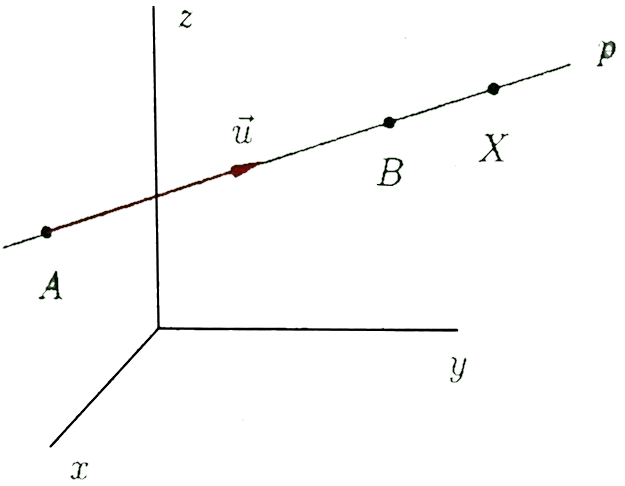
\includegraphics[width=0.4\linewidth]{mai_fig000.png}
    \captionof{figure}{Zadáni přímky. \cite[s.~1]{Musilova2009MA1}
    \label{mai:fig000}}
    \par}
  Veličinou \(t\), takzvaným \emph{parametrem}, který může nabývat všech reálných hodnot, 
  \(t\in\mathbb{R}\), dokážeme popsat všechny vektory \(\overrightarrow{AX}\), jejichž 
  koncový bod \(X\) leží na přímce \(p\). Naopak, žádné jiné body \(X\) než ty, které leží na 
  přímce \(p\), tuto vlastnost nemají. S označením bodů \(A\), \(X\), resp. vektorů 
  \(\vec{u}\), \(\overrightarrow{AX}\) kartézskými souřadnicemi, resp. složkami
  \begin{align*}
                    A &= (x_A,y_A, z_A), \\ 
                    X &=(x,y,z),         \\
              \vec{u} &= (u_1,u_2,u_3),  \\ 
  \overrightarrow{AX} &= (x - x_A, y - y_1A, z-z_A),
  \end{align*}
  dostáváme \textbf{parametrické vyjádřeni přímky} \(p\) ve tvaru
  \begin{equation}\label{MAI:eq_M001}
    p = \left\{(x,y,z)\in\mathbb{R}^3\,|\,
    \begin{matrix}
      x = x_A + tu_1,        \\
      y = y_A + tu_2,        \\
     z = z_A + tu_3,
    \end{matrix}
    \;t\in\mathbb{R}
    \right\}. 
  \end{equation}
  \normalsize
\end{example}
    %---------------------------------------------------------------
    
    Vidíme, že kartézské souřadnice bodu na přímce se vůči souřadnicím bodu \(A\) mění přímo 
    úměrně v závislosti na hodnotě parametru \(t\), tj. závisí na jeho první mocnině. Příslušná 
    závislost se nazývá \textbf{lineární funkcí}.
    
    Obdobně zapíšeme parametrické vyjádření roviny v \(\mathbb{R}^3\):
    
    %--Parametrická vyjádření roviny--------------------------------
    % !TeX spellcheck = cs_CZ
\begin{mathexam}{Parametrická vyjádření roviny}{exam004}
  Rovina v trojrozměrném prostoru \(\mathbb{R}^3\) je zadána třemi body \(A\), \(B\) a \(C\), které
  nesmějí ležet v jedné přímce, popřípadě dvěma body \(A\) a \(B\) a vektorem \(\vec{v}\)
  nerovnoběžným s \(\overrightarrow{AB}\), anebo bodem \(A\) a dvěma nerovnoběžnými směrovými
  vektory \(\vec{u}\) a \(\vec{v}\) (obr. \ref{mai:FIG002}). Všechny tyto typy zadání jsou
  ekvivalentní. Lze volit například \(\vec{u} = \overrightarrow{AB}\), \(\vec{v} =
  \overrightarrow{AC}\). Je-li \(X\) libovolným bodem roviny \(\varrho\), jsou vektory
  \(\overrightarrow{AX}\), \(\vec{u}\) a \(\vec{v}\) \textbf{lineárně závislé}. To znamená, že
  existují taková reálná čísla \(r\) a \(s\), že vektor \(\overrightarrow{AX}\) lze zapsat jako
  lineární kombinaci

  \begin{equation*}
    \overrightarrow{AX} = r\cdot\vec{u} + s\cdot\vec{v}, \qquad r,s \in\mathbb{R}
  \end{equation*}
  Při obdobném zápisu kartézských souřadnic bodů a složek vektorů jako u vyjádření přímky dostaneme
  parametrické vyjádření roviny \(\varrho\)
  \begin{equation*}
    \varrho = \left\{
    \begin{matrix}  
      (x,y,z)\in\mathbb{R}^3  \\
      r, s \in\mathbb{R}
    \end{matrix}
    \,\left\lvert\,
    \begin{matrix}
      x = x_A + ru_1 + sv_1,        \\
      y = y_A + ru_2 + sv_2,        \\
      z = z_A + ru_3 + sv_3,
    \end{matrix}\right.          
    \right\}.
  \end{equation*} 

  { \centering
    \captionsetup{type=figure}
    \luafigure[1]{mai_fig026.pdf}
    \captionof{figure}{Zadání roviny. \cite[s.~3]{Musilova2009MA1}
    \label{mai:FIG002}} \par}

  Toto vyjádření obsahuje opět lineární závislost: Souřadnice \(x\), \(y\) a \(z\) se vůči
  souřadnicím bodu \(A\) mění v závislosti na prvních mocninách parametrů \(r\) a \(s\). Můžeme tak
  hovořit o jakési „vícerozměrné úměře“.
\end{mathexam}
  
    %---------------------------------------------------------------
    
    Všimněme si nyní příkladů linearity z oblasti přírodovědy.
    
    %--Fyzika — Ohmův zákon-----------------------------------------
    % !TeX spellcheck = cs_CZ
% \wikitextrule
\begin{mdframed}[style=mdexam]
  \begin{example}\label{mai:exam035}
    \textbf{Fyzika - Ohmův zákon:}\newline
    Z elektřiny víme, že některé vodiče či elektrické prvky se při průchodu elektrického proudu 
    chovají podle zákona linearity: Proud, který jimi protéká, závisí přímo úměrně na přiloženém 
    napětí (obr. \ref{mai:fig036}). Platí \(I(U) = R^{-1 }U\) s konstantou úměrnosti \(R^{-1}\), kde 
    \(R\) je elektrický odpor vodiče (prvku).

    Pozn. 1: Předpokládáme, že elektrický odpor voltmetru je tak velký, že proud jím procházející je 
    z hlediska přesnosti měření zanedbatelný.
    
    Pozn. 2: Graf závislosti proudu na napětí na obrázku \ref{mai:fig036} může pro vyšší hodnoty 
    napětí vykazovat odchylku od linearity (přímkové závislosti), neboť se prvek při vyšším proudu 
    zahřívá a jeho odpor roste.
    
    {\centering
      \captionsetup{type=figure}
      \luafigure[1]{mai_fig036.png}
      \captionof{figure}{Chování lineárního vodiče (Ohmův zákon). \cite[s.~15]{Musilova2009MA1}
      \label{mai:fig036}}
      \par}  
  \end{example}
\end{mdframed}
    %---------------------------------------------------------------

    %--Fyzika — speciální typy pohybů-------------------------------
    % !TeX spellcheck = cs_CZ
\wikitextrule
\begin{example}\label{mai:exam036}
  \textbf{Fyzika — speciální typy pohybů:}\newline\small
  Při rovnoměrném pohybu tělesa (ať již přímočarém či křivočarém) je dráha, kterou těleso urazí za 
  dobu \(t\), přímo úměrná velikosti jeho rychlosti \(v\), tj. \(s(t) = s_0 + vt\). Při pohybu 
  rovnoměrně zrychleném (zpožděném) je lineární závislost velikosti rychlosti na čase, tj. \(v(t) = 
  v_0 \pm at\) při pohybu přímočarém (\(a\) je velikost zrychlení), nebo \(v(t) = v_0 \pm a_\tau 
  t\) při pohybu křivočarém (\(a_\tau\) je velikost průmětu zrychlení do směru tečny k 
  trajektorii tělesa — tečného zrychlení).
  \normalsize
\end{example}
    %---------------------------------------------------------------
    
  \subsection{Soustavy lineárních rovnic a jejich rychlé řešení}
    Příkladů linearity v přírodě bychom mohli nalézt bezpočet. Vraťme se však k matematice a k 
    problematice uvedené v názvu tohoto odstavce, k soustavám lineárních rovnic. Začněme 
    jednoduchou slovní úlohou ze základní školy:
    
    %--Jeníček a Mařenka kradli ježibabě perník---------------------
    % !TeX spellcheck = cs_CZ
% \wikitextrule
\begin{mdframed}[style=mdexam]
  \begin{example}\label{mai:exam037}
    \textbf{Jeníček a Mařenka kradli ježibabě perník:}\newline
    Dohromady snědli \num{11} perníkových srdíček. Jeníček jich přitom zkonzumoval o \num{3} více
    než Mařenka. Otázka je tradiční - kolik srdíček snědl každý z nich? Označíme-li \(M\) počet
    kousků, které snědla Mařenka a \(J\) počet srdíček, na nichž si pochutnal Jenda, můžeme
    informace zadané v úloze zapsat takto:
    \begin{equation*}
      M + J = 11, \qquad J = M + 3.
    \end{equation*}
    
    Řešení není problémem, snadno vidíme, že \(M = 4\) a \(J = 7\).
  \end{example}
\end{mdframed}
    %---------------------------------------------------------------
    
    O samotné řešení této jednoduché úlohy v tuto chvíli nejde. Pojmenujme si však vztahy, které 
    jsme pro neznámé hodnoty \(M\) a \(J\) ze zadání úlohy dostali. Neznámé vystupují v 
    rovnicích v první mocnině, tedy \emph{lineárně}. Máme \emph{soustavu dvou rovnic} o dvou 
    neznámých \(M\) a \(J\). Úvahu snadno zobecníme: Předpokládejme, že máme neznámé veličiny
    \begin{equation*}
      (x_1, x_2, \ldots, x_n)
    \end{equation*}
    a máme o nich \(m\) informací, které lze zapsat ve tvaru lineárních rovnic (neznámé budou v 
    těchto rovnicích vystupovat v první mocnině),
    \begin{align}
      a_{11}x_1 + a_{12}x_2 + \ldots + a_{1n}x_n &= b_1,     \nonumber           \\
      a_{21}x_1 + a_{22}x_2 + \ldots + a_{2n}x_n &= b_2,     \label{mai:eq002}   \\
      .......................................... &= \ldots   \nonumber           \\
      a_{m1}x_1 + a_{m2}x_2 + \ldots + a_{mn}x_n &= b_m,     \nonumber
    \end{align}
    Soustavu (\ref{mai:eq002}) nazýváme soustavou \(m\) lineárních rovnic o \(n\) neznámých. 
    Označme ji jako \(S\) a pod tímto označením se k ní budeme vracet. Soubory reálných čísel 
    \((a_{ij})\) a \((b_i)\), kde \(1 < i < m\), \(1 \leq j < n\), jsou zadány. Lze je uspořádat 
    do takzvaných \textbf{matic}:
    \begin{equation}\label{mai:eq003}
      \matr{A} =
        \begin{pmatrix}
          a_{11} & a_{12} & \ldots & a_{1n} \\
          a_{21} & a_{22} & \ldots & a_{2n} \\
          \ldots & \ldots & \ldots & \ldots \\
          a_{m1} & a_{m2} & \ldots & a_{mn}          
        \end{pmatrix},
        \overline{\matr{B}} =
        \begin{pmatrix}
          b_1     \\
          b_2     \\
          \ldots  \\
          b_m 
        \end{pmatrix}
    \end{equation}
    
    Matice \(\matr{A}\) je typu \(m/n\), má \(m\) řádků a \(n\) sloupců, \(i\) je řádkový index a 
    \(j\) je sloupcový index. Matice \(\overline{\matr{B}}\) je typu \(m/1\) (\(m\) řádků a jeden 
    sloupec), hovoříme také o sloupcové matici. Soustavu \(S\) můžeme zapsat zkráceně pomocí 
    maticového násobení (podrobněji viz později odstavec \ref{mai:IchapIIsecIII}):
    \begin{equation*}
      \matr{A} \cdot \matr{X} = \matr{B}, \qquad \text{nebo}
    \end{equation*}  
    \begin{equation}\label{mai:eq004}
        \begin{pmatrix}
          a_{11} & a_{12} & \ldots & a_{1n} \\
          a_{21} & a_{22} & \ldots & a_{2n} \\
          \ldots & \ldots & \ldots & \ldots \\
          a_{m1} & a_{m2} & \ldots & a_{mn}
        \end{pmatrix}
        \cdot
        \begin{pmatrix}
          x_1     \\
          x_2     \\
          \ldots  \\
          x_m 
       \end{pmatrix}
        =
       \begin{pmatrix}
            b_1     \\
            b_2     \\
            \ldots  \\
            b_m 
          \end{pmatrix}
    \end{equation}
    V tuto chvíli vysvětlíme podstatu maticového násobení jen technicky: Násobit mezi sebou  můžeme matici 
    \(\matr{A} = (a_{ij})\) typu \(m/n\) (levý činitel) a matici \(\matr{A} = (c_{jk})\) typu 
    \(n/p\) (pravý činitel, činitele nelze zaměňovat). Výsledkem je matice \(\matr{A} = (d_{ik})\) 
    typu \(m/p\), jejíž prvky se počítají podle předpisu
    \begin{equation}\label{mai:eq005}
      d_{ik} = \sum_{j=1}^{n} a_{ij}\cdot c_{jk}.
    \end{equation}
    
    Z tohoto obecného předpisu vidíme, že levé strany soustavy \(S\) lze interpretovat ve tvaru 
    součinu matice \(A\) typu \(m/n\) s maticí neznámých typu \((n/1)\), výsledkem je matice 
    pravých stran \(\overline{\matr{B}}\), která je typu \(m/1\). Matice \(\matr{A}\) se nazývá 
    \textbf{maticí soustavy}. Matice, která vznikne jejím \emph{rozšířením} o sloupec pravých 
    stran, tj.
    \begin{equation}\label{mai:eq006}
      \matr{B} = (\matr{A}|\overline{\matr{B}}) =
      \left(
        \begin{array}{cccc|c}
          a_{11} & a_{12} & \ldots & a_{1n} & b_1    \\
          a_{21} & a_{22} & \ldots & a_{2n} & b_2    \\
          \ldots & \ldots & \ldots & \ldots & \ldots \\
          a_{m1} & a_{m2} & \ldots & a_{mn} & b_m
        \end{array}
      \right)
    \end{equation}
    je pak \textbf{rozšířenou maticí soustavy}. Je-li sloupec pravých stran soustavy tvořen 
    samými nulami, nazývá se soustava \textbf{homogenní}, v opačném případě \textbf{nehomogenní}. 
    Řešením soustavy \(S\) nazýváme každou \(n\)-tici \((x_i, x_2,\ldots, x_n)\), která soustavu 
    \(S\) splňuje. Cílem je najít všechna řešení soustavy \(S\). Abychom řešení nalezli, musíme 
    soustavu upravovat, zjednodušovat. Prováděné úpravy mají vést k jednodušší, avšak 
    ekvivalentní soustavě rovnic, tj. takové, která má naprosto stejný soubor všech řešení jako 
    soustava původní. Takové úpravy nazýváme \textbf{ekvivalentními}. Dvě základní, pomocí nichž 
    lze uskutečnit všechny ostatní, jsou
    \begin{itemize}\addtolength{\itemsep}{-0.5\baselineskip}
      \item vynásobení libovolné, například \(i\)-té, rovnice libovolným \emph{nenulovým} číslem,
      \item přičtení \(i\)-té rovnice vynásobené libovolným číslem k \(l\)-té rovnici.
    \end{itemize} 
    V soustavě lze samozřejmě také měnit pořadí rovnic. Tato úprava je rovněž ekvivalentní. 
    Nevypisujeme ji však zvlášť proto, že ji lze realizovat pomocí vhodně zvolené posloupnosti 
    základních dvou úprav.
    
    Abychom nemuseli soustavu stále opisovat i s neznámými, provádíme obvykle ekvivalentní 
    úpravy jen s maticí \(\matr{B} = (\matr{A}|\overline{\matr{B}})\) (každý řádek této matice 
    představuje jednu rovnici soustavy \(S\)). Může se stát, že soustava má právě \emph{jedno 
    řešení}, jako tomu bylo v  úloze o Mařence a Jeníčkovi. Také nemusí mít \emph{řešení žádné}, 
    jako například soustava \(x + y = 0\), \(x + y = 1\) (součet dvou čísel nemůže nabývat současně 
    dvou různých hodnot). A třeba má také řešení \emph{nekonečně mnoho} (řešením soustavy jedné 
    rovnice o dvou neznámých \(x + y = 1\) jsou všechny dvojice tvaru \((x, 1 - x)\), kde \(x\) je 
    libovolné). A může mít soustava \(S\) třeba právě dvě řešení? Prostřednictvím následujícího 
    příkladu ukážeme metodu, která vede velmi rychle k nalezení všech řešení a umožňuje také 
    vyslovit obecné závěry o jejich vlastnostech a počtu. Jedná se o \textbf{Gaussovu eliminační 
    metodu}.

    %Gaussova eliminační metoda-------------------------------------
    \begin{mathexam}{Gaussova eliminační metoda}{exam038}
  Je zadána soustava tří (\(m = 3\)) rovnic o pěti (\(n = 5\)) neznámých:
  \begin{alignat*}{7}
       x_1 &+ 2x_2 &-  x_3 &+  x_4 &- 5x_5 &=  &&0, \\
     -2x_1 &- 4x_2 &+ 2x_3 &+ 4x_4 &+ 4x_5 &= -&&6, \\
      -x_1 &- 2x_2 &+  x_3 &+ 5x_4 &-  x_5 &=  &&6.
  \end{alignat*}
  Budeme provádět ekvivalentní úpravy matice \(\matr{B}\) tak, abychom ji zjednodušovali.
  Ekvivalenci matic budeme označovat znakem \(\sim\). 
  \begingroup
    \renewcommand\arraystretch{1.0}
    \renewcommand\arraycolsep{3pt}
    \begin{equation*}
      \matr{B} = (\matr{A}\lvert\overline{\matr{B}}) =
      \left(
        \begin{array}{rrrrr|r}
           1 &  2 & -1 & 1 & -5 &  0    \\
          -2 & -4 &  2 & 4 &  4 & -6    \\
          -1 & -2 &  1 & 5 & -1 &  6
        \end{array}
      \right).
    \end{equation*}
  \endgroup
  V prvním řádku je na první pozici jednička. Toho využijeme k snadné „likvidaci“, tedy eliminaci,
  prvních prvků v druhém a třetím řádku pomocí elementárních úprav. Provedeme tyto dvě úpravy:
  první řádek vynásobený číslem \num{2} přičteme k druhému řádku, první řádek přičteme ke třetímu
  řádku. Dostaneme
  \begingroup
    \renewcommand\arraystretch{1.0}
    \renewcommand\arraycolsep{3pt}
    \begin{equation*}
      \matr{B} \sim
      \left(
        \begin{array}{rrrrr|r}
          1 &  2 & -1 & 1 & -5 &  0         \\
          \bm{0} &  0 &  0 & 6 & -6 & -6    \\
          \bm{0} &  0 &  0 & 6 & -6 &  6
        \end{array}
      \right).
    \end{equation*}
  \endgroup  
  Vidíme, že jsme v druhém i třetím řádku dostali na první sloupcové pozici nulu (tučná). (Nuly na
  dalších  pozicích vznikly náhodou, vlivem jednoduchosti zadání.) Nyní vynásobíme druhý i třetí
  řádek číslem (\num{1/6}):
  \begingroup
    \renewcommand\arraystretch{1.0}
    \renewcommand\arraycolsep{3pt}    
    \begin{equation*}
      \matr{B} \sim
      \left(
        \begin{array}{rrrrr|r}
                1 &  2 & -1 & 1 & -5 &  0    \\
                0 &  0 &  0 & 1 & -1 & -1    \\
                0 &  0 &  0 & 1 & -1 &  1
        \end{array}
      \right).
    \end{equation*}
  \endgroup  
  Přestože již nyní vidíme, že soustava nemá řešení (rovnice druhého a třetího řádku znějí \(x_4 -
  x_5 = - 1\) a \(x_4 -x_5 = 1\), takže jim nevyhovuje žádná dvojice čísel \((x_4, x_5)\)), budeme
  v eliminaci pokračovat. Další úpravy se již týkají pouze druhého a třetího řádku. Druhý řádek
  vynásobený (\num{-1}) přičteme ke třetímu. Pak

  \begingroup
  \renewcommand\arraystretch{1.0}
  \renewcommand\arraycolsep{3pt}
    \begin{equation*}
      \matr{B} \sim
      \left(
        \begin{array}{rrrrr|r}
                1 &  2 & -1 & 1      & -5 &  0    \\
                0 &  0 &  0 & 1      & -1 & -1    \\
                0 &  0 &  0 & \bm{0} &  0 &  2
        \end{array}
      \right).
    \end{equation*}
  \endgroup  
  Získáváme tak ekvivalentní soustavu rovnic
  \begin{alignat*}{5}
        x_1 + 2x_2 - x_3 &+  x_4 &- 5x_5 &=  &&0, \\
                         &+  x_4 &-  x_5 &= -&&1, \\
                         &       &     0 &=  &&2.
  \end{alignat*}
  V poslední rovnici je ihned vidět rozpor - soustava nemá řešení
\end{mathexam}
    %---------------------------------------------------------------

    Na základě výsledného tvaru matice soustavy a rozšířené matice soustavy získané ekvivalentními 
    úpravami soustavy \(S\) nyní formulujeme obecné kritérium pro to, aby soustava S měla
    vůbec nějaké řešení. Matice \(\matr{A}\) i \(\matr{B}\) se po provedení ekvivalentních úprav 
    dostaly do velmi jednoduchého tvaru, který připomíná schodiště obrácené „vzhůru nohama“, 
    odmyslíme-li si nuly v levé části jednotlivých řádků (následující zápis pouze usnadňuje 
    názornou představu, znak ekvivalence již psát nemůžeme):
    \begin{equation*}
      \matr{A} \ldots
      \left(
        \begin{array}{rrrrr}
                1 &  2 & -1 & 1      & -5     \\
                  &    &    & 1      & -1     \\
 
        \end{array}
      \right),
      \qquad
      \matr{B} \ldots
      \left(
        \begin{array}{rrrrr|r}
                1 &  2 & -1 & 1      & -5 &  0    \\
                  &    &    & 1      & -1 & -1    \\
        \end{array}
      \right).
    \end{equation*}
    
    Všimněme si, že „schodiště“ jsou nepravidelná, pokud jde o šířku schodů, výška všech schodů
    je však stejná - jeden řádek. Tímto způsobem je dán \emph{schodovitý tvar} matice \(\matr{A}\), 
    resp. \(\matr{B}\). Úzce s ním souvisí důležitá charakteristika matice, která je nezávislá jak 
    na provedených úpravách tak na výsledném schodovitém tvaru. Je to hodnost matice, definovaná 
    takto:
    
    \textbf{Hodnost} matice je počet nenulových řádků jejího schodovitého tvaru.
    
    V našem příkladu je hodnost matice \(A\) soustavy \(S\) rovna dvěma, hodnost matice rozšířené 
    \(\matr{B}\) je rovna třem. Píšeme
    \begin{equation*}
      h(\matr{A}) = 2,\qquad h(\matr{B}) = 3.
    \end{equation*}
    
    \begin{note}
      Lze získat schodovitý tvar různými posloupnostmi ekvivalentních úprav je zřejmé. Uvědomme si 
      však, že ani výsledný schodovitý tvar není určen jednoznačně - stačí třeba vynásobit některý 
      řádek dvěma a výsledná matice ekvivalentní s původní je rovněž schodovitá. Poněvadž má matice 
      \(\matr{B}\) o jeden sloupec více než matice \(\matr{A}\), platí vždy \(h(\matr{A}) < 
      h(\matr{B})\). V případě \(h(\matr{A}) < h(\matr{B})\) pak \(h(\matr{A}) = h(\matr{B}) - 1\). 
      Jak názorně ukazuje náš příklad, má pro \(h(\matr{A}) < h(\matr{B})\) některá z rovnic 
      ekvivalentní soustavy tvar \(0 = 1\), soustava tedy nemá řešení. Můžeme tak formulovat 
      kritérium (podmínku nutnou a postačující) řešitelnosti soustavy lineárních rovnic.
    \end{note}
    
    \begin{lemma}\label{mai:lemma001}
      (\textbf{Frobeniova}): Soustava lineárních rovnic má řešení právě tehdy, je-li hodnost její 
      matice rovna hodnosti matice rozšířené.
    \end{lemma}
    
    Ihned vidíme, že homogenní soustava má podle této věty řešení vždy, neboť poslední sloupec její 
    rozšířené matice je složen ze samých nul. Skutečně, jedním ze souboru řešení každé
    homogenní soustavy je \(n\)-tice
    \begin{equation*}
      (x_1, x_2, \ldots, x_n) = (0, 0, \ldots, 0),
    \end{equation*}
    zvaná \textbf{triviální řešení}.
    
    Nyní se vraťme k otázce, jak zjistit, kolik řešení má daná soustava, a jak je všechna popsat.
    Poslouží nám příklad \ref{mai:exam038} v mírné obměně spočívající v záměně koeficientu \(b_3\) 
    z hodnoty \num{6} na \num{-6}.
    
    %Ještě jednou Gaussova eliminační metoda------------------------
    % !TeX spellcheck = cs_CZ
\wikitextrule
\begin{example}\label{mai:exam039}
  \textbf{Ještě jednou Gaussova eliminační metoda}\newline\small
  Je zadána soustava rovnic:
  \begin{alignat*}{7}
      x_1 &+ 2x_2 &-  x_3 &+  x_4 &- 5x_5 &=  &&0, \\
    -2x_1 &- 4x_2 &+ 2x_3 &+ 4x_4 &+ 4x_5 &= -&&6, \\
     -x_1 &- 2x_2 &+  x_3 &+ 5x_4 &-  x_5 &= -&&6.
  \end{alignat*}
  Rozšířená matice soustavy má nyní tvar 
  \begin{equation*}
    \matr{B} = (\matr{A}|\overline{\matr{B}}) =
    \left(
      \begin{array}{rrrrr|r}
         1 &  2 & -1 & 1 & -5 &  0    \\
        -2 & -4 &  2 & 4 &  4 & -6    \\
        -1 & -2 &  1 & 5 & -1 & -6
      \end{array}
    \right).
  \end{equation*}
  Stejné ekvivalentní úpravy jako v příkladu \ref{mai:exam038} vedou nyní k výsledku
  \footnotesize %\small \scriptsize \tiny
  \begin{equation*}
    \matr{B} \sim
    \left(
      \begin{array}{rrrrr|r}
         1 &  2 & -1 & 1 & -5 &  0         \\
         \bm{0} &  0 &  0 & 6 & -6 & -6    \\
         \bm{0} &  0 &  0 & 6 & -6 & -6
      \end{array}
    \right) \sim
    \left(
      \begin{array}{rrrrr|r}
              1 &  2 & -1 & 1 & -5 &  0    \\
              0 &  0 &  0 & 1 & -1 & -1    \\
              0 &  0 &  0 & 1 & -1 & -1
      \end{array}
    \right) \sim
    \left(
      \begin{array}{rrrrr|r}
              1 &  2 & -1 & 1      & -5 &  0    \\
              0 &  0 &  0 & 1      & -1 & -1    \\
              0 &  0 &  0 & \bm{0} &  0 &  0
      \end{array}
    \right).
  \end{equation*}\normalsize
  Nyní platí \(h(\matr{A}) = h(\matr{B}) = 2\). Podle Frobeniovy věty \ref{mai:lemma001} tedy 
  soustava určitě má řešení. Ekvivalentní soustava má tvar
  \begin{alignat*}{5}
         x_1 + 2x_2 - x_3 &+  x_4 &- 5x_5 &=  &&0, \\
                          &+  x_4 &-  x_5 &= -&&1, \\
                          &       &     0 &=  &&0.
  \end{alignat*}
  Poslední rovnice je identitou a můžeme ji vypustit. Máme pět neznámých a jen dvě nezávislé 
  rovnice. Dvě z neznámých tedy můžeme vyjádřit pomocí zbývajících. Postupujeme „odzadu“ , začínáme 
  druhou, jednodušší, rovnicí:
  \begin{align*}
                                                x_4 &= -1 + x_5,                \\
    x_1 = - 2x_2 + x_3 - x_4 + 5x_5 \Rightarrow x_1 &= -2x_2 + x_3 + 4x_5 + 1.
  \end{align*}
  Za neznámé vystupující na pravé straně, tj. \(x_2\), \(x_3\) a \(x_5\), můžeme dosazovat cokoli a 
  vždycky se k nějakým hodnotám \(x_1\) a \(x_4\) dopočítáme. Všechna řešení soustavy \(S\) proto 
  můžeme zapsat v obecném tvaru
  \begin{equation}\label{mai:eq040}
    (-2x_2 + x_3 + 4x_5 + 1, x_2, x_3, x_5 - 1, x_5).
  \end{equation}
  \normalsize
\end{example}
    %---------------------------------------------------------------
    
    Soubor řešení ve tvaru (\ref{mai:eq040}) se nazývá obecným řešením soustavy. Jeho jednotlivé 
    prvky, jednotlivá konkrétní řešení soustavy, jsou dány volbou volných neznámých \(x_2\), 
    \(x_3\) a \(x_5\). Také z příkladu \ref{mai:exam039} lze učinit obecný závěr:
    
    \begin{lemma}\label{mai:lemma002}
      Nechť pro soustavu \(m\) lineárních rovnic o \(n\) neznámých platí \(h(\matr{A}) = 
      h(\matr{B}) = h\). Pak její obecné řešení závisí (lineárně) na \(d = n - h\) volných 
      neznámých.
    \end{lemma}
    
    Číslo \(d\) se nazývá \textbf{dimenze prostoru řešení soustavy}. Tento pojem ještě podrobněji 
    vysvětlíme později.
    
    Nyní již snadno zodpovíme otázku, čím je dána mohutnost souboru řešení soustavy lineárních 
    rovnic, tj. kolik má taková soustava řešení. Možnosti jsou pouze:
    \begin{itemize}
      \item žádné řešení - pro \(h(\matr{A}) \neq h(\matr{B})\),
      \item právě jedno řešení - pro \(h = h(\matr{A}) = h(\matr{B})\) a současně \(h = n\), takže 
            nezbývá žádná volná neznámá,
      \item nekonečně mnoho řešení - pro \(h = h(\matr{A}) = h(\matr{B})\) a současně \(h < n\),  
            kdy máme k dispozici \(d = n - h\) volných neznámých.
    \end{itemize}    
    Že by tedy třeba měla soustava právě dvě, tři či osmnáct řešení není možné.
    
    Jakési zvláštní postavení můžeme přisoudit homogenním soustavám. Ty mají, jak jsme se
    již přesvědčili, řešení vždy, alespoň to triviální, složené ze samých nul. Zajímejme se o 
    situaci, kdy má homogenní soustava i jiná, netriviální, řešení. U homogenní soustavy je 
    hodnost její matice vždy shodná s hodností matice rozšířené, \(h = h(\matr{A}) = h(\matr{B})\). 
    Je-li navíc \(h = n\), má podle obecného tvrzení \ref{mai:lemma002} soustava právě jedno 
    řešení, jímž nutně je řešení triviální. V opačném případě, tj. pro \(h < n\), máme opět k 
    dispozici \(d = n - h\) volných neznámých, a tedy nekonečně mnoho netriviálních řešení. 
    Všimněme si ještě jedné zajímavosti u homogenní soustavy. Jsou-li dvě \(n\)-tice čísel \(X = 
    (x_1, x_2, \ldots, x_n)\) a \(\overline{X} = (\overline{x}_1, \overline{x}_2, \ldots, 
    \overline{x}_n)\) jejím řešením, pak také \(n\)-tice vytvořená jako jejich lineární kombinace
    \begin{equation*}
      \alpha\cdot X + \overline{\alpha}\cdot\overline{X} = 
        (\alpha x_1, \alpha x_2, \ldots, \alpha x_n) + 
        (\overline{\alpha}\,\overline{x}_1, 
        \overline{\alpha}\,\overline{x}_2, \ldots, 
        \overline{\alpha}\,\overline{x}_n)
    \end{equation*}
    kde \(\alpha\) a \(\overline{\alpha}\) jsou libovolná čísla, je \emph{řešením soustavy}. 
    Možnost tohoto „lineárního kombinování“ připadá samozřejmě v úvahu pro libovolný počet 
    libovolných řešení soustavy. Fyzik by řekl, že soustava vyhovuje principu superpozice. 
    Soustava nehomogenní tu to vlastnost nemá „vinou“ nenulového sloupce 
    pravých stran.
    
    \subsection{Přímky a roviny - lineární geometrické útvary}
      Vraťme se ještě na chvíli k linearitě v geometrii a všimněme si problematiky vzájemné polohy
      přímek a rovin. Procvičíme si na ní mimo jiné i řešení soustav lineárních rovnic. V odstavci 
      \ref{mai:IchapIIsecI} jsme odvodili parametrické vyjádření přímky a roviny v trojrozměrném 
      prostoru. Nyní se pokusíme z těchto vyjádření vyloučit parametry a získat obecné rovnice 
      přímky a roviny, které již budou obsahovat pouze kartézské souřadnice bodů ležících v 
      příslušné přímce či rovině. Začněme případem roviny.

      %--Obecná rovnice roviny----------------------------------------
      % !TeX spellcheck = cs_CZ
\wikitextrule
\begin{example}\label{mai:exam040}
  \textbf{Obecná rovnice roviny}\newline\small
  Parametrické rovnice roviny z příkladu \ref{mai:exam004} můžeme chápat jako soustavu tří rovnic o 
  dvou neznámých:
  \begin{align*}
      ru_1 + sv_1 &= x - x_A, \\
      ru_2 + sv_2 &= y - y_A, \\
      ru_3 + sv_3 &= z - z_A, 
  \end{align*}
  kde neznámými jsou parametry \(r\) a \(s\). Z geometrického významu této soustavy je zřejmé, že 
  pro každý bod \(X = (x, y, z)\), který leží v rovině \(\varrho\), bude soustava mít jako řešení 
  právě jednu dvojici parametrů \((r, s)\) (pro body, které v rovině neleží, soustava řešení nemá). 
  Vypočteme parametry \(r\) a \(s\) například z prvních dvou rovnic. Předpokládejme, že \(u_1 \neq 
  0\), a upravujme matici soustavy:
  
  \begin{equation*}
    \left(
      \begin{array}{rr|r}
         u_1 &  v_1  &  x-x_A         \\
         u_2 &  v_2  &  y-y_A
      \end{array}
    \right) \sim
    \left(
      \begin{array}{cc|c}
              u_1 &  v_1               & x - x_A     \\
              0   &  u_1v_2 - u_2v_1   & (y-y_A)u_1 - (x-x_A)u_2
      \end{array}
    \right).
  \end{equation*}
  odkud pro \((u_1v_2 — u_2v_1) \neq 0\) dostaneme
  \begin{equation*}
    r = - \dfrac{(y-y_A)v_1 - (x-x_A)v_2}{u_1v_2 - u_2v_1}, \qquad 
    s =   \dfrac{(y-y_A)u_1 - (x-x_A)u_2}{u_1v_2 - u_2v_1}
  \end{equation*}
  Dosadíme-li získané hodnoty do třetí rovnice (dá to trochu práce), dostáváme obecnou  rovnici roviny 
  \(\varrho\)
  \begin{subequations} % \label{mai:eq041}
    \begin{equation}\label{mai:eq041a}
      ax + by + cz + d= 0,
    \end{equation}
    \begin{equation}\label{mai:eq04b}
      a = u_2v_3 - u_3v_2, \qquad b = u_3v_1 - u_1v_3, \qquad c = u_1v_2 - u_2v_1,
    \end{equation}
    \begin{equation}\label{mai:eq041c}
      d = (u_2v_3 - u_3v_2)x_A - (u_3v_1 - u_1v_3)y_A - (u_1v_2 - u_2v_1)z_A.
    \end{equation}
  \end{subequations}
  Při tomto výpočtu vyvstaly některé problémy. Pokusme se je vyřešit:
  \begin{itemize}
    \item Aby získaná rovnice opravdu představovala nějakou rovinu, musí v ní zůstat alespoň jedna 
          ze souřadnic \(x, y, z\). Alespoň jedno z čísel \(a, b, c\) by tedy mělo být nenulové. 
          Dokažte, že tomu tak opravdu je, a využijte při tom skutečnosti, že vektory \(\vec{u}\) a 
          \(\vec{v}\) nesmí být rovnoběžné. Co znamená předpoklad \((u_1v_2 - u_2v_1) \neq 0\)?
    \item Předpokládali jsme, že \(u_1 \neq 0\). Jak budeme postupovat, nebude-li tento předpoklad  
          splněn? Lze v tomto případě použít obecné výrazy získané pro \(r\) a \(s\)?
  \end{itemize}
  \normalsize
\end{example}
      %---------------------------------------------------------------

      %--Obecná rovnice přímky----------------------------------------
      % !TeX spellcheck = cs_CZ
% \wikitextrule
\begin{mdframed}[style=mdexam]
  \begin{example}\label{mai:exam041}
    \textbf{Obecná rovnice přímky}\newline
    Přímku \(p\) si snadno představíme jako průsečnici dvou nerovnoběžných rovin \(\varrho\) a 
    \(\sigma\). Jejich rovnice tvoří soustavu, která představuje obecné rovnice přímky
      \begin{align*}
        \varrho &= \{(x, y, z)\in\mathbb{R}^3\mid a_1x+ b_1y+ c_1z+ d_1 = 0 \}  \\ 
        \sigma  &= \{(x, y, z)\in\mathbb{R}^3\mid a_2x+ b_2y+ c_2z+ d_2 = 0 \}, 
      \end{align*}
    Zkusme přijít na to, co musí platit pro koeficienty v rovnicích rovin, aby byly nerovnoběžné. 
    Jedna a táž přímka může být zadána různými dvojicemi nerovnoběžných rovin. Všechny roviny, které 
    přímkou \(p\) procházejí, tvoří geometrický útvar zvaný \textbf{svazek rovin prvního druhu}, 
    přímka sama je \textbf{osou} svazku. 
  \end{example}
\end{mdframed}
      %---------------------------------------------------------------
      
      %--Vektor rovnoběžný s rovinou----------------------------------
      % !TeX spellcheck = cs_CZ
\wikitextrule
\begin{example}\label{mai:exam042}
  \textbf{Vektor rovnoběžný s rovinou}\newline\small
   Ja k poznáme, zda je vektor \(\vec{u} = (u_1, u_2, u_3)\) rovnoběžný s rovinou \(ax + by + cz + 
   d = 0\)? Pokud vektor \(\vec{u}\) s rovinou rovnoběžný je, pak zcela jistě existují v této 
   rovině dva body \(A = (x_A, y_A, z_A)\) a \(B = (x_B, y_B, z_B)\) tak, že \(\overrightarrow{AB} 
   = \vec{u} = (x_B - x_A, y_B - y_A, z_B - z_A)\). Tyto body splňují rovnici roviny, tj.
   \begin{equation*}
     ax_A + by_A + cz_A + d = 0,\qquad ax_B + by_B + cz_B + d = 0.
   \end{equation*}
   Odečtením rovnic dostaneme kritérium rovnoběžnosti vektoru s rovinou \(au_1 + bu_2+ cu_3 = 0\).
   \normalsize
\end{example}
      %---------------------------------------------------------------
  
      Máme připraveno vše pro řešení otázky vzájemné polohy přímek a rovin.

      %--Vzájemná poloha tří rovin------------------------------------
      % !TeX spellcheck = cs_CZ
\wikitextrule
\begin{example}\label{mai:exam043}
  \textbf{Vzájemná poloha tří rovin}\newline\small
  Zapojme geometrickou představivost a uvažujme, jakou vzájemnou polohu mohou mít tři roviny
  \begin{align*}
    \varrho: a_1x + b_1y + c_1z + d_1 &= 0, \\
    \sigma : a_2x + b_2y + c_2z + d_2 &= 0, \\
    \tau   : a_3x + b_3y + c_3z + d_3 &= 0,
  \end{align*}
  Současně si uvědomme, že předchozí soustava je soustavou lineárních rovnic o neznámých \(x\), 
  \(y\) a \(z\), představujících souřadnice společných bodů rovin \(\varrho\), \(\sigma\) a 
  \(\tau\). Soustava je charakterizována maticí
  \begin{equation}\label{mai:eq043}
    \matr{B} = (\matr{A}|\overline{\matr{B}}) =
    \left(
      \begin{array}{rrr|r}
         a_1 & b_1 & c_1 & -d_1    \\
         a_2 & b_2 & c_2 & -d_2    \\
         a_3 & b_3 & c_3 & -d_3
      \end{array}
    \right).
  \end{equation}
  Jsou tyto možnosti:
  \begin{itemize}
    \item Roviny mají společný právě jeden bod. V tomto případě musí mít soustava (\ref{mai:eq043}) 
          právě jedno řešení, a tedy \(h(\matr{A}) = h(\matr{B}) = 3\). (Útvar, který by vytvořily 
          všechny roviny procházející tímto bodem, se nazývá \textbf{trs rovin prvního druhu}, 
          společný bod je vrchol trsu.)
    \item Roviny mají společnou přímku. Řešení soustavy (\ref{mai:eq043}) bude v takovém případě 
          závislé na jedné volné neznámé (parametr bodů na společné přímce), takže \(h(\matr{A}) = 
          h(\matr{B}) = 2\). (Útvar, který by vytvořily všechny roviny procházející touto přímkou, 
          jsme před chvílí nazvali \textbf{svazkem rovin prvního druhu}, společná přímka je 
          \textbf{osou} svazku.)
    \item Roviny jsou totožné. Řešení soustavy (\ref{mai:eq043}) je popsáno dvěma volnými neznámými 
          (parametry bodů ve společné rovině), je tedy \(h(\matr{A}) = h(\matr{B}) = 1\).
    \item Roviny nemají společný žádný bod, mají však společný právě jeden směr (představme si 
          například nekonečně dlouhý stan „áčko“, v němž jedna z rovin tvoří podlážku a zbylé dvě 
          jsou stěnami). Společný směr \(\vec{u}\) je řešením homogenní soustavy rovnic (příklad 
          \ref{mai:exam043})
          \begin{align}\label{mai:eq044}
            a_1u_1 + b_1u_2+ c_1u_3 &= 0, \\
            a_2u_1 + b_2u_2+ c_2u_3 &= 0, \\
            a_3u_1 + b_3u_2+ c_3u_3 &= 0.
          \end{align}
           jejíž řešení musí být popsáno jednou volnou neznámou, tj. \(h(\matr{A}) = 2\). Původní 
           nehomogenní soustava (\ref{mai:eq043}) pro společné body rovin však řešení nemá, je tedy 
           \(h(\matr{B}) = 3\). (Útvar, který by vytvořily všechny roviny obsahující společný směr, 
           se nazývá \textbf{trs rovin druhého druhu}.)
    \item Roviny jsou rovnoběžné, nemají však žádný společný bod. Znamená to, že mají společné 
          dva nezávislé směry, řešení homogenní soustavy (\ref{mai:eq044}) obsahuje dvě volné 
          neznámé a platí \(h(\matr{A}) = 1\), \(h(\matr{B}) = 2\).
  \end{itemize}
  \normalsize
\end{example}
      %---------------------------------------------------------------

      %--Vzájemná poloha dvou přímek----------------------------------
      % !TeX spellcheck = cs_CZ
\wikitextrule
\begin{example}\label{mai:exam044}
  \textbf{Vzájemná poloha dvou přímek}\newline\small
  Dvě přímky \(p\) a \(q\) jsou určeny dvěma dvojicemi rovin. Jejich společné body jsou tedy 
  řešením soustavy čtyř lineárních rovnic o třech neznámých (pišme rovnou rozšířenou matici 
  soustavy):
  \begin{equation}\label{mai:eq045}
    \matr{B} = (\matr{A}|\overline{\matr{B}}) =
    \left(
      \begin{array}{rrr|r}
         a_1 & b_1 & c_1 & -d_1    \\
         a_2 & b_2 & c_2 & -d_2    \\
         a_3 & b_3 & c_3 & -d_3    \\
         a_4 & b_4 & c_4 & -d_4
      \end{array}
    \right).
  \end{equation}
  Protože soustava obsahuje rovnice dvojic nerovnoběžných rovin, je \(h(\matr{A}) \geq 2\) 
  (zdůvodněte podrobněji). Možnosti vzájemné polohy přímek \(p\) (první dvě rovnice) a \(q\) (druhé 
  dvě rovnice) jsou tyto:
  \begin{itemize}
    \item Přímky jsou mimoběžné, nemají tedy žádný společný bod a roviny, které je určují, nemají 
          žádný společný směr. Soustava (\ref{mai:eq045}) nemá řešení, odpovídající homogenní 
          soustava pak rovněž ne, kromě řešení triviálního. Je tedy \(h(\matr{A}) = 3\), 
          \(h(\matr{B}) = 4\).
    \item Přímky jsou různoběžné, mají tedy společný právě jeden bod. Soustava (\ref{mai:eq045}) má 
          právě jedno řešení, a proto \(h(\matr{A}) = h(\matr{B}) = 3\).
    \item Přímky jsou rovnoběžné. Nemají tedy žádný společný bod, soustava nemá řešení, ale roviny, 
          které je určují, mají společný směr. To odpovídá situaci \(h(\matr{A}) = 23\), 
          \(h(\matr{B}) = 3\).
    \item Přímky jsou totožné. Řešení soustavy je popsáno jednou volnou neznámou, tj. \(h(\matr{A}) 
          = h(\matr{B}) = 2\)
  \end{itemize}
  \normalsize
\end{example}
      %---------------------------------------------------------------
      
      %--Vzájemná poloha přímky a roviny------------------------------
      % !TeX spellcheck = cs_CZ
\wikitextrule
\begin{example}\label{mai:exam045}
  \textbf{Vzájemná poloha přímky a roviny}\newline\small
  Tuto úlohu převeďme na problém vzájemné polohy tří rovin a odpovězme si sami. Společně vyřešíme 
  konkrétní případ. Rozhodněme o vzájemné poloze přímky a roviny, najděme jejich společné body a 
  směry:
  \begin{align*}
    p       &: x + y + z + 5 = 0, \qquad 2x + 3y + 6z - 10 = 0 \\
    \varrho &: y + 4z + 17   = 0.
  \end{align*}
  \begin{equation*}
    \matr{B} = (\matr{A}|\overline{\matr{B}}) =
    \left(
      \begin{array}{rrr|r}
         1 & 1 & 1 & -5    \\
         2 & 3 & 6 &  10   \\
         0 & 1 & 4 & -17
      \end{array}
    \right)\sim
    \left(
      \begin{array}{rrr|r}
         1 & 1 & 1 & -5    \\
         0 & 1 & 4 &  20   \\
         0 & 1 & 4 & -17
      \end{array}
    \right)\sim
    \left(
      \begin{array}{rrr|r}
         1 & 1 & 1 & -5    \\
         0 & 1 & 4 &  20   \\
         0 & 0 & 0 & -37
      \end{array}
    \right).
  \end{equation*}
  Matice \(\matr{A}\) i \(\matr{B}\) jsme upravili do schodovitého tvaru. Vidíme, že \(h(\matr{A}) 
  = 2\), \(h(\matr{B}) = 3\). Soustava nemá řešení přímka \(p\) a rovina \(\varrho\) nemají žádný 
  společný bod. Jediná možnost, jak to zařídit, je, že přímka \(p\) je s rovinou \(\varrho\) 
  rovnoběžná. Mají společný směr, který je řešením homogenní soustavy o matici
  \begin{equation*}
    \matr{A} =
    \left(
      \begin{array}{ccc}
         1 & 1 & 1   \\
         2 & 3 & 6   \\
         0 & 1 & 4 
      \end{array}
    \right)\sim
    \left(
      \begin{array}{ccc}
         1 & 1 & 1   \\
         0 & 1 & 4   \\
         0 & 0 & 0 
      \end{array}
    \right).
  \end{equation*}
  Schodovitý tvar matice odpovídá ekvivalentní soustavě rovnic
  \begin{equation*}
    u_1 + u_2 + u_3 = 0,\qquad u_2 + 4u_3 = 0,
  \end{equation*}
  jejíž řešení je tvaru \((u_1, u_2, u_3) = (3u_3, -4u_3, u_3)\). Společný směr přímky \(p\) a 
  roviny \(\varrho\) je tedy určen například směrovým vektorem \((3, -4, 1)\) (pro \(u_3 = 1\)) 
  nebo kterýmkoli jeho nenulovým násobkem.
  \normalsize
\end{example}
      %---------------------------------------------------------------
      
%--------------------------------------------------------------------------------------------------
  \section{Počítání s čísly}\label{mai:IchapIIsecII}
    Někdo se jistě pozastaví nad tím, že jej chceme učit počítání s čísly. To přece každý umí
    už od základní školy! Jenže základní a do značné míry i střední škola nás učí počítat jen
    s určitým typem čísel - s čísly reálnými. Pravidla pro počítání s nimi se pro „běžné uživatele“
    stala natolik rutinní záležitostí, že už o nich vůbec nepřemýšlejí, nehledají v nich 
    zákonitosti, a kdybychom se jich zeptali, kde se tato pravidla vzala, pravděpodobně budou s 
    odpovědí velmi váhat. Pravidla pro jakékoli početní operace totiž skutečně nelze z ničeho 
    odvodit, ta je třeba definovat, samozřejmě tak, aby měla rozumné praktické vlastnosti.
    
    \subsection{Reálná čísla}
      U reálných čísel se opravdu dlouho nezdržíme, s těmi snad opravdu každý umí počítat. Všimneme 
      si jen trochu podrobněji struktury množiny všech reálných čísel, \textbf{reálné osy} 
      \(\mathbb{R}\). Zobrazit  reálná čísla na reálné ose, tedy na přímce, umíme proto, že na 
      množině reálných čísel je definováno \textbf{úplné uspořádání} „< “:
      \begin{itemize}
        \item Je-li současně \(a ≤ b\) a \(b ≤ a\), pak \(a = b\) 
              pro všechna \(a, b\in\mathbb{R}\ldots\) \textbf{antisymetrie},
        \item je-li současně\( a ≤ b\) a \(b ≤ c\), pak \(a ≤ c\) 
              pro všechna \(a,b,c\in\mathbb{R}\ldots\) \textbf{tranzitivita},
        \item \(a ≤ a\) pro všechna \(a\in\mathbb{R}\ldots\) \textbf{reflexivita},
        \item platí \(a ≤ b\) nebo \(b ≤ a\) pro všechna \(a, b \in\mathbb{R}\ldots\) 
              \textbf{úplnost}.
      \end{itemize}
      Pro každá dvě čísla \(a\) a \(b\) tedy dokážeme rozhodnout, zda jsou shodná (\(a = b\)), nebo 
      zda \(a\) je menší (\(a < b\)) či větší (\(a > b\)) než \(b\). Platí:
      \begin{itemize}
        \item Je-li současně \(a < b\) a \(c < d\), pak \(a + c < b + d\),
        \item je-li současně \(a < b\) a \(c > 0\), pak \(ac < bc\),
        \item je-li současně \(a < b\) a \(c < 0\), pak \(ac > bc\).
      \end{itemize}
      
      Množina reálných čísel obsahuje tyto důležité podmnožiny:
      \begin{itemize}
        \item Množinu přirozených čísel \(\mathbb{N} = \{1, 2, \ldots, n, \ldots\}\). Platí princip 
              \textbf{úplné indukce}: Je-li \(\mathbb{M} \subseteq \mathbb{N}\) nějaká množina 
              přirozených čísel, která obsahuje číslo \num{1} a která současně s každým číslem 
              \(n\) obsahuje i \(n + 1\), pak \(\mathbb{M} = \mathbb{N}\).
        \item Množinu celých čísel \(\mathbb{Z} = \{\ldots, -n, \ldots, -2, -1, 0, 1, 2, \ldots, m, 
              \ldots\}\).
        \item Množinu racionálních čísel \(\mathbb{Q}\) (zlomky). Racionální čísla lze vyjádřit 
              konečnými desetinnými zlomky (například \(p/q = 1/4 = \num{0.25}\)), nebo nekonečnými 
              periodickými desetinnými zlomky (například \(p/q = 4/3 = 1,33\ldots33\ldots = 
              1,\overline{3}\), \(p/q = 24/11 = 2,1818\ldots1818\ldots = 2,\overline{18}\)).
        \item Množinu iracionálních čísel, tj. čísel, která nejsou racionální. Iracionálními čísly 
              jsou neracionální řešení algebraických rovnic, například \(x^2 - 2 = 0 \Rightarrow x 
              = \sqrt{2}\), nebo \(x = - \sqrt{2}\) (čísla algebraická), a čísla typu \(\pi\), 
              \(e\), atd. (čísla transcendentní). Iracionální čísla jsou vyjádřena       
              nekonečnými neperiodickými desetinnými zlomky, např. 
              \(e = \num{2.718281828459545}\ldots\). Mezi každými dvěma reálnými čísly leží 
              nekonečně mnoho čísel racionálních i nekonečně mnoho čísel iracionálních.
      \end{itemize}
      
      Pro počítání s reálnými čísly jsou zavedeny základní operace, s nimiž umíme pracovat na
      základě zkušenosti, sčítání \(a + b\), odčítání \(a - b\), násobení \(a \cdot b\), resp. 
      \(ab\) a dělení \(a : b\). Ve skutečnosti jsou potřeba jen dvě, neboť odčítání je odvozeno 
      pomocí sčítání a dělení pomocí násobení. Uvědomili jste si někdy základní vlastnosti těchto 
      operací? Možná ne, ale pracujeme s nimi zcela samozřejmě:
%      \begin{table}[ht!]
%        \centering
%%        \begin{tabular}{l>{\centering}m{5cm}} %{@{}ll@{}}
%%\begin{tabular}{| c | >{\centering}m{5cm} |}
%%        \toprule
%%          \(a + b = b + a\)            & komutativní zákon pro součet  \\ %\midrule
%%          \((a + b) + c = a + (b +c)\) & asociativní zákon pro součet  \\
%%          \(a + 0 = 0 + a = a\)        & existence univerzálního neutrálního prvku \num{0}  \\
%%          \(a + (—a) = (—a) + a = 0\)  & existence právě jednoho opačného prvku k číslu \(a\)   \\ 
%%          \(ab = ba\)                  & komutativní zákon pro součin \\
%%          \(a(bc) — (ab)c\)            & asociativní zákon pro součin \\
%%          \(a(b + c) = ab + ac\)       & 1. distributivní zákon  \\
%%          \((b+ c)a — ba + ca\)        & 2. distributivní zákon \\
%%          \(a \cdot 1 = 1 \cdot a\)    & existence univerzálního jednotkového prvku 1 \\
%%          \(aa^{-1} = a^{-1}a\)        & existence právě jednoho inverzního prvku k číslu \(a\), pokud 
%%                                         \(a\neq 0\)\\
%%          \(ab = 0 \Leftrightarrow a = 0\) nebo \(b = 0\)) & neexistence dělitelů nuly \\
%%         \bottomrule
%%        \end{tabular}
%%\begin{tabular}{| c | >{\centering}m{5cm} |}
%% Bcd & A long cell with text that wraps around and is centered
%%\end{tabular}
%      \end{table}
      Odčítání a dělení:
      \begin{equation*}
        a — b = a + (—b), a:b = ab^{-1}, \qquad\text{pokud } b\neq0.
      \end{equation*}
      
    \subsection{Komplexní čísla}
      Komplexními čísly rozumíme uspořádané dvojice \([x, y]\) čísel reálných, pro které zavedeme 
      určité operace. Uspořádaností dvojice zde myslíme to, že jedno z čísel (v našem zápisu \(x\)) 
      je umístěno na první pozici dvojice a představuje reálnou část čísla \(z\), \(x = 
      \operatorname{Re}(z)\), druhé (v našem zápisu \(y\)) je na druhé pozici a je imaginární částí 
      čísla \(z\), \(y = \operatorname{Im}(z)\). Je tedy obecně  \( [x, y] ≠ [y, x]\). Množinu
    \subsection{Cvičení}
%--------------------------------------------------------------------------------------------------
  \section{Počítání s maticemi}\label{mai:IchapIIsecIII}
    \subsection{Základní operace s maticemi a hodnost matic}\label{mai:IchapIIsecIIIsubI}
    \subsection{Hodnost matic}\label{mai:IchapIIsecIIIsubII}
    \subsection{Násobení  matic}\label{mai:IchapIIsecIIIsubIII}
    \subsection{Čtvercová matice}\label{mai:IchapIIsecIIIsubIV}
    Algebra matic, tedy počítání s nimi, je v praxi zase jen počítání s čísly, samozřejmě podle
    specifických pravidel. S maticemi jsme se již setkali v odstavci \ref{mai:IchapIIsecI}, kde 
    jsme jich využili jako vhodné „pomůcky“ při řešení soustav rovnic. Nyní posuneme naše 
    znalosti o nich na poněkud vyšší úroveň. Zavedeme na množině matic \emph{algebraickou 
    strukturu}, která nám umožní s nimi počítat nezávisle na jejich vztahu k nějakým praktickým 
    aplikacím. Víme již, že maticí typu \(m/n\) (též obdélníková matice) rozumíme soubor reálných, 
    popřípadě i komplexních čísel uspořádaných do \(m\) řádků a \(n\) sloupců:
    
    \begin{definition}\label{def_matice}
      Nechť \(m, n\) jsou přirozená čísla. Jestliže každé uspořádané dvojici \((m,n)\in 
      \{1,2,\ldots,m\}\times \{1,2,\ldots,m\}\) přiřadíme prvek \(a_{i,j}\in\mathbb{R}\) obdržíme 
      reálnou \href{http://cs.wikipedia.org/wiki/Matice}{matici} typu \(m,n\) nad \(\mathbb{R}\). 
      
      Matici zapisujeme jako
      \begin{equation}\label{matice_zapis}
        \matr{A} = \left(a_{ij}\right) =\left(
                                      \begin{array}{ccc}
                                        a_{11} & \ldots & a_{1n} \\
                                        \vdots & \ddots & \vdots \\
                                        a_{m1} & \ldots & a_{nn}
                                      \end{array}
                                 \right)
      \end{equation}
      která má právě \(mn\) prvků \((a_{ij})\) uspořádaných do \(m\) řádků a \(n\) sloupců. Stručně 
      píšeme \(\matr{A} = (a_{ij})\)
    \end{definition}

    Prvky matice jsou označeny indexy udávajícími \textbf{řádek} a \textbf{sloupec}, v nichž se 
    prvek nalézá. Prvek v \(i\)-tém řádku a \(j\)-tém sloupci matice \(\matr{A}\) se obvykle značí 
    \(a_{ij}\). Potom \(i\)-tý řádek matice  obsahuje vodorovnou \(n\)-tici prvků \(a_{i1}, 
    a_{i2}, \ldots,a_{in} \), kde \(i=  1,2,\ldots,m\) a \(j\)-tý sloupec matice obsahuje svislou 
    matici čísel \(a_{1j},a_{2j},\ldots,a_{mj}\), kde \(j = 1,2,\ldots,n\). Pro \(m = n\) se matice 
    nazývá čtvercová n-tého řádu. 
      
    %---------------------------------------------------------------
    % !TeX spellcheck = cs_CZ
% \wikitextrule
\begin{mdframed}[style=mdexam]
  \begin{example}\label{mai:exam033}
    Matice \(\begin{pmatrix*}[r]1&2&3&4\\4&3&2&1\\-1&-1&-1&-1\\-2&-1&0&1\end{pmatrix*}\) je čtvercová 
    matice velikosti \(4\times4\). Prvek matice \(a_{23}\) je \(2\).
  \end{example}
\end{mdframed}
    %---------------------------------------------------------------

    V tabulce \ref{LA:tab_basic_matrix} jsou uvedeny nejčastější typy matic, které se v algebře 
    často vyskytují. Jsou to například matice řádkové, sloupcové, diagonální\footnote{Prvky 
    \(a_{ii}\) kde \(i=1,2,\ldots,\min(m,n)\) tvoří hlavní diagonálu. Matice \(\matr{D}\) je 
    typu \(m,m\), obecně může mít diagonální matice buď ještě další sloupce, v nichž budou samé 
    nuly, anebo další řádky, v nichž budou opět samé nuly.}, jednotkové\footnote{Jestliže \(m = 
    n\), pak mluvíme o čtvercové matici řádu \(m\).}, nulové, transponované a symetrické.

    \begin{table}[!ht]
        \centering
        \renewcommand{\arraystretch}{1.8}   % for the vertical padding
          \begin{tabular}{|l||c@{}|}              
            \hline 
            \textbf{Matice}                    & \textbf{Zápis} \\ \hline\hline
            \ttfamily řádková   \(\matr{A}\) &  \(a_1,a_2,\ldots,a_n \)\\
            \ttfamily sloupcová \(\matr{B}\) & 
              \(\begin{pmatrix}
                a_1     \\
                a_2     \\
                \vdots  \\
                a_n
              \end{pmatrix}\)                       \\
            \ttfamily diagonální \(\matr{C}\) & 
              \(\begin{pmatrix}
                 a_{11} &    0   & \ldots &   0     \\
                    0   & a_{22} & \ldots &   0     \\
                 \vdots & \vdots & \ddots & \vdots  \\
                    0   &   0    & \ldots & a_{mm}
              \end{pmatrix}\)                       \\
            \ttfamily jednotková \(\matr{I}\) &
              \(\begin{pmatrix}
                   1    &    0   & \ldots &   0    \\
                   0    &    1   & \ldots &   0    \\
                 \vdots & \vdots & \ddots & \vdots \\
                    0   &   0    & \ldots & 1
              \end{pmatrix}\)                      \\
            \ttfamily nulová \(\matr{0}\) & \((a_{ij}),\quad a_{ij} = 0\,\forall\,i, j\) \\
            \ttfamily transponovaná \(\matr{D^T}\) &
              \(\begin{pmatrix}
                a_{11} & a_{21} & \ldots &  a_{m1}\\
                a_{12} & a_{22} & \ldots &  a_{m2}\\
                \vdots & \vdots & \ddots & \vdots \\
                a_{1n} & a_{2n} & \ldots & a_{mn}
              \end{pmatrix}\)    \\
            \ttfamily symetrická \(\matr{S}\) 
            & \((a_{ij}),\quad a_{ij}= a_{ji}\,\forall\,i,j\) \\ \hline
          \end{tabular}
        \caption{Speciální typy matic}\label{LA:tab_basic_matrix}
    \end{table}
  
  
    Matice téhož typu \((m,n)\) nad \(\mathbb{R}\) budeme značit \(\mathbb{R}_{m,n}\).
      
    \subsection{Základní operace s maticemi a hodnost matic}
      
      
    \begin{definition} 
      Součinem matice \(A \in \mathbb{R}_{mn}\) a matice \(B \in \mathbb{R}_{np}\), v uvedeném
      pořadí, je matice \(C \in \mathbb{R}_{mp}\) pro kterou platí:
      \begin{align*}
             C &= AB; \quad C = (cij); \\
             \shortintertext{kde}
        c_{ij} &= \sum_n^{k=1}{a_{ik}b_{kj}};\quad
                   i = 1,\ldots,m; \, j = 1,\ldots,p.
      \end{align*} 
    \end{definition}
    Součin matic \(A\) a \(B\) je definován právě tehdy, když počet sloupců matice \(A\) je roven 
    počtu řádků matice \(B\). Obrázek \ref{LA:fig_LA001a} demonstruje jakým způsobem se 
    dostane prvek, který je ve výsledné matici třeba ve druhém řádku a druhém sloupci, násobením 
    druhého řádku levé matice s druhým sloupcem pravé ze zadaných matic. Stejným způsobem získáme 
    hodnotu prvku \(c_{ij}\) (viz \ref{LA:fig_LA001b}).
    %----------------------------------
    \begin{figure}[ht!]
      \centering  
      \begin{tabular}{cc}
        \subfloat[1. krok]{\label{LA:fig_LA001a}
          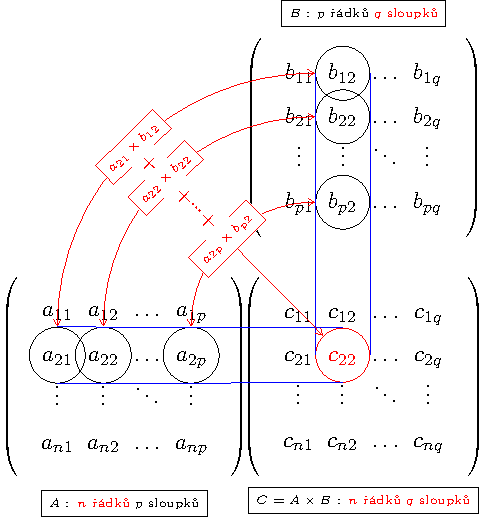
\includegraphics[width=0.45\linewidth]{mai_fig023a}}               &
        \subfloat[2. krok]{\label{LA:fig_LA001b}
          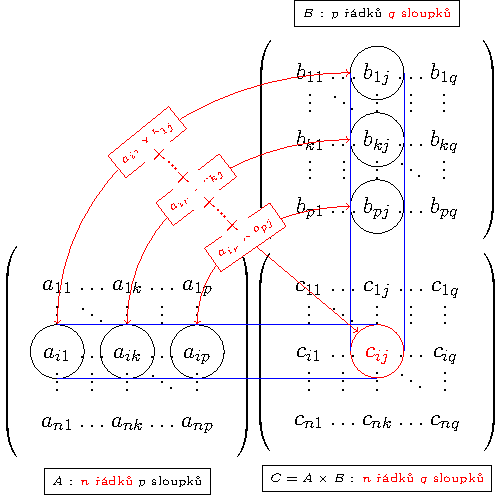
\includegraphics[width=0.45\linewidth]{mai_fig023b}} 
      \end{tabular}
      \caption{Postup při maticovém násobení}
    \end{figure}
  

      
      \begin{definition}\label{rovnost_matic}
       (Rovnost matic):  Matice \(\matr{A} = \left(a_{ij}\right)\) je rovna matici \(\matr{B}=
       \left(b_{kl}\right)\), jsou-li matice stejného typu a stejnolehlé prvky se sobě
       \textbf{rovnají}, tj. \(\matr{A} \in \mathbb{R}_{m,n}, \matr{B}\in\mathbb{R}_{m,n}, 
       a_{ij} = b_{ij}, \forall i\in\lbrace1,2,\ldots,m\rbrace, \forall j\in\lbrace1,2, \ldots 
       ,n\rbrace\).
      \end{definition}
      
%--------------------------------------------------------------------------------------------------
  \section{Počítání s vektory}\label{mai:IchapIIsecIV}
    \textbf{Vektory} budeme nazývat matice typu \(1/n\) a značit je
    \begin{equation*}
      \vec{u} = (u_1, u_2, \ldots, u_n).
    \end{equation*}
    Takže počítat s nimi již umíme! (V zápisu složek vektoru je vynechán řádkový index. V případě 
    matice s jedním řádkem, takzvané \emph{řádkové matice}, je totiž zbytečný.) Číslům \(u_1\) až 
    \(u_n\) budeme pro tuto chvíli říkat \emph{složky vektoru} \(\vec{u}\). Za chvíli tento pojem 
    ještě upřesníme. Celou řadu pojmů, s nimiž jsme se seznámili při počítání s maticemi, můžeme 
    pro vektory přímo použít. Namísto značení \(\mathcal{M} (1/n)\) budeme pro prostor vektorů 
    používat symbol \((\mathbb{R}^n)\) nebo \(\mathbb{C}^n\) (obvyklý symbol pro množinu 
    uspořádaných \(n\)-tic reálných nebo komplexních čísel).
    
    \subsection{Součiny vektorů}
      Kromě základních operací s vektory, tj. sčítání vektorů a násobení vektoru skalárem, se 
      často používají další operace, které obohacují \emph{strukturu vektorového prostoru}. 
      Zůstaneme u vektorů v trojrozměrném prostoru \(\mathbb{R}^3\) a definujeme si skalární, 
      vektorový a smíšený součin vektorů. Skalární součin vektorů definujeme prostřednictvím 
      geometrické definice jako zobrazení, které uspořádané dvojici vektorů (volných vektorů nebo 
      jejich libovolných umístění) přiřazuje reálný číslo podle předpisu
      \begin{equation}\label{mai:eq038}
        \vec{u}\vec{v} = \abs{\vec{u}}\cdot\abs{\vec{v}}\cos\varphi,
      \end{equation}
      kde \(\varphi = \sphericalangle(\vec{u},\vec{v})\) je velikost minimálního z obou úhlů mezi 
      vektory\(\vec{u},\vec{v}\).

    %---------------------------------------------------------------
    % !TeX spellcheck = cs_CZ
% \wikitextrule
\begin{mdframed}[style=mdexam]
  \begin{example}\label{mai:exam034}
    Vypočteme z definice \ref{mai:eq038} skalární součiny vektorů ortonormální báze \(\vec{e_1}\), 
    \(\vec{e_2}\) a \(\vec{e_3}\), spjaté s kartézskou soustavou souřadnic. Připomeňme, že tyto 
    vektory jsou jednotkové a navzájem kolmé.
    \begin{itemize}
      \item pro \(i\neq j\) \(\vec{e_i}\vec{e_j}=0\), 
                \(\sphericalangle\vec{e_i}\vec{e_j} =\dfrac{\pi}{2}\), vektory jsou kolmé,
      \item pro \(i = j\) \(\vec{e_i}\vec{e_j}=0\), 
                \(\sphericalangle\vec{e_i}\vec{e_j} =0, \abs{\vec{e_i}}=1\), vektory jsou 
                jednotkové.
    \end{itemize}

    Pro skalární součiny vektorů ortonormální báze použijeme zkrácené značení
    \begin{equation}\label{mai:eq085}
      \vec{e_i}\vec{e_j} = \delta_{ij},
    \end{equation}
    kde \(\delta_{ij}\) nabývá hodnoty \num{1} pro \(i = j\) a hodnoty \num{0} pro \(i \neq j\). 
    Nazývá se \textbf{Kroneckerovo delta} \cite[s.~40]{Musilova2009MA1}.
  \end{example}
\end{mdframed}
    %---------------------------------------------------------------
    
    Shrneme nyní vlastnosti skalárního součinu. Dokázat bychom je mohli, i když by to mohlo být i 
    velmi pracné, užitím znalostí z goniometrie. Zkuste to alespoň pro jednu z nich! Třeba se    
    vám podaří zvolit si tu nejjednodušší.

%} % tikzset
%---------------------------------------------------------------------------------------------------
\printbibliography[title={Seznam literatury}, heading=subbibliography]
\addcontentsline{toc}{section}{Seznam literatury}
  % !TeX spellcheck = cs_CZ
% Differential calculus
%{\tikzset{external/prefix={tikz/MAI/}}
% \tikzset{external/figure name/.add={ch03_}{}}
%---------------------------------------------------------------------------------------------------
% Limits_of_Functions.tex
%---------------------------------------------------------------------------------------------------
\chapter{Limita a spojitost funkce}\label{mai:IchapLimit}
\minitoc

  %================Podkapitola: Reálná funkce ======================================================
  \section{Reálná funkce}
    %-----------------------------------------------------------------------------------------------
    \small
    S funkcemi se setkáváme na každém kroku nejen ve fyzice a v ostatních přírodních vědách, ale i 
    v každodenním životě. Každá situace, kdy jsou nějaký jev či veličina jednoznačně a nevyhnutelně 
    určeny jinými jevy či veličinami, se dá popsat pomocí funkce\footnote{V matematice abstrahujeme 
    při zkoumání funkcionálních závislostí od konkrétní fyzikální povahy proměnných veličin a 
    chápeme je jako \uv{bezrozměrné veličiny}, tedy jako číselné proměnné. Někdy je jednoduché 
    takovou} funkci sestavit. Snadno například můžeme zjistit, jakou dráhu urazí automobil jedoucí 
    známou rychlostí v závislosti na tom, jak dlouho jede. Nebo dokážeme určit přírůstek našich 
    úspor ve spořitelně v závislosti na době spoření, pokud známe úrokovou míru a její změny. Jindy 
    je naopak skoro nemožné přijít na to, jak taková funkce vypadá, neboť nemáme dostatek informací 
    o parametrech, které do jejího zápisu vstupují. Třeba takovou závislost teploty ovzduší v daném 
    okamžiku na zeměpisné poloze a nadmořské výšce, kterou bychom si mohli představit jako jednu ze 
    samozřejmých součástí předpovědi počasí, bychom asi nesestavili. Popis jevů pomocí funkcí je v 
    každém případě velmi užitečný. Má však svá pravidla, s nimiž se v této kapitole seznámíme. 
    Závisí-li zkoumaný jev nebo veličina na jediné veličině, jejíž hodnoty jsou reálné a buď se 
    mění známým způsobem, nebo si je můžeme dokonce volit, hovoříme o \textbf{funkci jedné reálné 
    proměnné}. A lze-li zkoumaný jev nebo veličinu kvantifikovat rovněž pomocí reálných hodnot, 
    jedná se o \textbf{reálnou funkci jedné reálné proměnné}. Právě o takových funkcích bude v této 
    kapitole řeč. V aplikacích se budeme věnovat především funkcím, které mají význam ve fyzice a v 
    přírodních vědách. Velmi často půjde o funkce, kde reálnou proměnnou je čas. Jevy v přírodě 
    podléhají totiž principu příčinnosti, a tak lze velké množství veličin popisujících přírodní 
    jevy vyjádřit na základě znalosti přírodních zákonů jako funkce času. 
    \cite[s.~53]{Musilova2009MA1}
    \normalsize
    \subsection{Funkce a její graf}\label{MAI:section_002}
      V tomto odstavci se naučíme funkce zadávat, počítat s nimi a vyjádřit je velmi přehledným 
      způsobem — jejich \emph{grafem}. Zopakujme, že každou \textbf{reálnou funkci}, jejíž 
      definiční obor je podmnožina množiny \(\realset\), nazýváme \textbf{reálnou funkcí jedné 
      reálné proměnné}\footnote{Místo názvu \uv{reálná funkce jedné reálné proměnné} budeme pro 
      stručnost používat pouze název \uv{funkce}, pokud nebude řečeno něco jiného}.
      
      Protože \emph{funkce je speciální případ zobrazení}, můžeme všech\-ny pojmy a obecné 
      vlastnosti zobrazení přenést i na funkce. Některé z nich však vzhledem k důležitosti 
      zopakujme, případně doplníme. Na druhé straně budeme studovat také ty vlastnosti, které jsou 
      specifické pro tento speciální druh zobrazení.
      
      \begin{note}
        Je-li \(\mathcal{D}_f = \naturalset\), jedná se o \textbf{posloupnost}. (Speciálním 
        případem reálných funkcí jedné reálné proměnné jsou \emph{posloupnosti reálných čísel)}.
      \end{note}
      
      \subsection{Způsoby zadání funkce}\label{MAI:section_000}
        Nejprve funkci definujeme. Předpokládejme, že reálná proměnná, na níž bude záviset náš jev, 
        má dovoleno nabývat hodnot z určité předem stanovené podmnožiny \(D\subseteq\realset\) 
        reálných čísel. Předpokládejme dále, že podle určitého pravidla, předpisu, dokážeme pro 
        \emph{každou hodnotu} \(x\) množiny \(\mathcal{D}_f\), tj. \(x \in \mathcal{D}_f\), určit 
        \emph{právě jednu} reálnou hodnotu \(y\). Každé hodnotě \(x \in D\) tedy nějaké \(y\) 
        příslušet \emph{musí},  avšak žádné hodnotě \(x\) \emph{nesmíme} přiřadit více hodnot 
        \(y\). Tak vzniká funkce \(f\). Hodnoty \(x\) se nazývají hodnotami \emph{nezávisle 
        proměnné} (neboli \emph{argumentu}), hodnoty \(y\) hodnotami \emph{závisle proměnné} a 
        \(f\) symbolizuje \emph{funkční předpis}. Píšeme
        \begin{equation}\label{mai:eq000}
            f: x \in \mathcal{D}_f \rightarrow y=f(x)\in\realset
        \end{equation}
      Hodnoty proměnné \(x\) nazýváme též \emph{vzory}, odpovídající hodnoty \(y = f(x)\) 
      \emph{obrazy}. Množina  \(\mathcal{D}_f\) je \emph{definičním oborem} funkce \(f\). Zadání 
      definičního oboru je důležitou součástí zadání funkce. Množina \(H\) všech takových reálných 
      hodnot \(y\), které jsou obrazem nějakého vzoru, 
      \begin{equation}\label{mai:eq001}
          \mathcal{H}_f = 
              \left\lbrace 
                y\in\realset\text{ existuje } x\in \mathcal{D}_f, \text{ tak že } y = f(x)  
              \right\rbrace, 
      \end{equation}
      se nazývá \emph{obor hodnot} funkce \(f\). Hodnotu \(f(x)\) nazýváme také \emph{funkční 
      hodnotou} funkce \(f\) v bodě \(x\). 

      \begin{figure}[ht!] %\ref{mai:fig001}
        \centering
%        % Funkce jako „černá skříňka“. \cite[s.~54]{Musilova2009MA1}

\documentclass[11pt]{standalone}
\usepackage{xltxtra}
\usepackage{tikz}
\usepackage{amsmath}

\begin{document}
  \begin{tikzpicture}[fill=black!20]
%  \draw[help lines] (-1,-2) grid (6,3);
    \path (0,0) node(a) [ ] {\(\mathcal{D}_f\)}
    (2,0) node(b) [rectangle,rotate=0,draw,fill] {\(\begin{array}{c} \text{funkce} \\ f(x)  
    \end{array}\)}
    (4,0) node(c) [ ] {\(\mathcal{H}_f\)};
    \draw[thick,->] (a.east) -- (b);
    \draw[thick,->] (b.east) -- (c);
    \path [ ] (a.east) -- (b.west)   node [above,midway] {\(x\)};
    \path [ ] (b.east) -- (c.west)   node [above,midway] {\(y\)};
  \end{tikzpicture}

\end{document}
        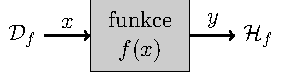
\includegraphics[width=0.45\linewidth]{mai_fig001.pdf}
        \caption{Funkce jako „černá skříňka“. \cite[s.~54]{Musilova2009MA1}}
        \label{mai:fig001}
      \end{figure}
      
      Funkci si podle obrázku \ref{mai:fig001} můžeme představit jako „černou skříňku“, do které 
      vstoupí hodnota (vzor) a vystoupí z ní hodnota \(y = f(x)\) (obraz). Množinu uspořádaných 
      dvojic čísel \([x, f(x)]\) nazveme \hyperref[MAI:section_001]{grafem funkce}.
      
      Jak zadat předpis \(f\)? Lze to udělat kterýmkoli z následujících způsobů, podle vhodnosti
      nebo snadnosti. Ukážeme jednotlivé možnosti na jednoduchém příkladu, kdy chceme hodnotám 
      proměnné \(x\) z množiny \(\mathcal{D}_f\) přiřadit jejich druhé mocniny. Zvolme pro náš 
      příklad definiční obor výčtem:
      \begin{equation*}
         \mathcal{D}_f = \lbrace-3,2,-1,0,1,2,3,4\rbrace,
      \end{equation*}
      a zadáme předpis
      \begin{itemize}\addtolength{\itemsep}{-0.5\baselineskip}
        \item \textbf{slovním popisem}: předpis \(f\) přiřazuje každé z hodnot \(x\in 
              \mathcal{D}_f\) její druhou mocninu,
        \item \textbf{vzorcem}: \(y = x^2\) pro \(x\in \mathcal{D}_f\) zadává zobrazení
              \begin{equation*}
                f: x\in \mathcal{D}_f \rightarrow f(x)= x^2\in\realset,
              \end{equation*}
        \item \textbf{tabulkou}: Hodnoty obrazů pro všechny vzory z \(\mathcal{D}_f\) vypíšeme do 
              tabulky:
              \begin{table}[h]
                \centering
                \begin{tabular}{c|rrrrrrrr}
                  \textbf{x} & -3 & -2 & -1 & 0 & 1 & 2 & 3 & 4  \\ \hline
                  \textbf{y} & 9  & 4  & 1  & 0 & 1 & 4 & 9 & 16
                \end{tabular}
                % \caption{ }
              \end{table}
              Proměnná $x$ se v tomto případě mění \uv{diskrétně}. Je zřejmé, že tímto způsobem 
              můžeme funkci definovat úplně jen tehdy, je-li definiční obor konečná množina. 
              Tabulku však používáme i v jiných případech, zejména chceme-li vyznačit pomocí ní, 
              některé hodnoty, které nás z nějakého důvodu přednostně zajímají. 
        \item Zadání \textbf{grafem}: 
          \begin{equation*}
            G_f = \left\lbrace\left[x,f(x)\right] |x\in D\right\rbrace
                = \left\lbrace\left[x,x^2 \right] |x\in D\right\rbrace
          \end{equation*}
          tak, že dvojice \([x, f(x)]\) znázorníme jako body v rovině (obr. \ref{MAI:fig_011}).
          \begin{figure}[ht!]
            \centering  
            \begin{tabular}{cc}
              \subfloat[ ]{\label{MAI:fig_011}
                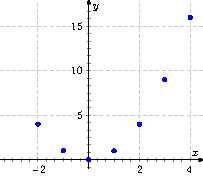
\includegraphics[width=0.4\linewidth]{mai_fig002.pdf}}              &
              \subfloat[ ]{\label{MAI:fig_010}
                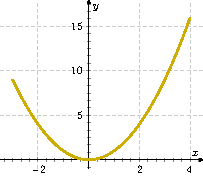
\includegraphics[width=0.4\linewidth]{mai_fig003.pdf}}              \\
            \end{tabular}
            \caption{Zadání funkce grafem}
          \end{figure}
          Z grafu můžeme ovšem funkční hodnoty určit pouze přibližně. Pro další matematické 
          zpracování je grafické zadání nejméně vhodné, i když jeho praktický význam například v 
          technických aplikacích nelze popřít.
        \item Zadání pomocí \textbf{rovnice}, jíž je funkce řešením: některé funkce nelze jednoduše 
              zapsat pomocí některého z předchozích způsobů, nebo to alespoň nejde přesně. Lze však 
              zapsat (diferenciální) rovnici, kterou tato funkce splňuje. Jedná se většinou o 
              speciální funkce, jimž se v tomto textu nebudeme věnovat. (Někdy může být taková 
              rovnice  představující zadání funkce i velmi jednoduchá. Například dosti známá funkce 
              \(\erf(x)\), \emph{error funkce}, velmi úzce souvisí s funkcí \(f(x) = 
              \frac{2}{\sqrt{x}}e^{-x^2}\). Nelze ji však zapsat vzorcem. Některé její hodnoty v 
              nejčastěji používaném rozsahu proměnné \(x\) můžeme najít v rozsáhlých tabulkách, 
              které byly sestaveny pomocí numerických metod.)
      \end{itemize}
      
      Již bylo zmíněno, že zadání definičního oboru je neopominutelnou součástí zadání funkce. 
      Kdybychom například zadali funkci opět předpisem \(y=x^2\), avšak za definiční obor stanovili 
      uzavřený interval \(D = \lbrace —3,4\rbrace\), dostali bychom graf na obrázku 
      \ref{MAI:fig_010}. Jde skutečně o jinou funkci než na obrázku \ref{MAI:fig_011}. Její úplnou 
      tabulku bychom nedokázali napsat vůbec.
      
%      Nejčastější způsob zadání funkce představuje \emph{vzorec}. Tabulku alespoň pro některé 
%      hodnoty z \(\mathcal{D}_f\) si pak dokážeme sestavit a schematický graf nakreslit. Někdy se 
%      objeví zadání funkce jen v podobě vzorce, například: „Je dána funkce \(y = f(x)\).“ Znamená 
%      to, že autor zapomněl zadat definiční obor? Nemusí tomu tak být. Tento způsob zadání chápeme 
%      tak, že si sami musíme stanovit „co největší“ definiční obor této funkce, tj. určit množinu 
%      všech takových \(x\), pro která lze do vzorce dosadit a hodnotu \(y\) určit.

      Zobrazovací předpis, kterým je funkce zadána, může být rozmanitý. Nejčastěji a pro účely 
      matematické analýzy nejvhodnější je \emph{analytické zadání vzorcem}, tj. rovnicí tvaru 
      $y=f(x)$ nebo několika takovými rovnicemi platnými pro různé části definičního oboru. Přitom 
      v rovnici $y=f(x)$ je na pravé straně nějaký správně definovaný výraz obsahující nejvýše 
      proměnnou $x$ a nabývající jednoznačné hodnoty pro danou hodnotu proměnné $x$.
      
%      Někdy však používáme (poněkud nedůsledně) termíny \uv{funkce \(f(x)\)} nebo \uv{funkce 
%      \(y=f(x)\)}. V tomto smyslu nepojímáme již \(x\) jako pevný prvek z definičního oboru, ale 
%      jako \uv{nezávisle proměnnou} neboli \emph{argument}, tj. symbol zastupující libovolný prvek 
%      z definičního oboru. V tomto případě pak písmeno \(y\) v rovnici \(y=f(x)\) nazýváme 
%      \emph{závisle proměnnou} a říkáme, že \uv{\(y\) závisí na \(x\)}. Tato frazeologie má své 
%      historické kořeny; tento způsob vyjádření funkce budeme využívat zřídka, zejména tam, kde 
%      nechceme pro označení příslušné funkce zavádět zvláštní symbol. Tak např. budeme mluvit o 
%      funkci \(e^x\) (ačkoliv se zavádí pro exponenciální funkci symbol exp) nebo o funkci \(\sin 
%      x\) (ačkoliv by bylo důslednější mluvit o funkci \(\sin\)) apod. \cite[s.~82]{Brabec1989} 

    %-------------------------------------
      % !TeX spellcheck = cs_CZ
\begin{mdframed}[style=mdexam]
  \begin{example}\label{MAI:exam017}
    (Definiční obor a obor hodnot funkce): Určíme „co největší“ definiční obor funkce
    \(y=\log_2{(\sqrt{1-x^2})}\) a zjistíme také její obor hodnot.
        
    {\centering
    \captionsetup{type=figure}
  %   % !TeX spellcheck = cs_CZ
% exam017.tex
% K příkladu \ref{fyz:fey_exam017} \(y=\log_2{(\sqrt{1-x^2})}\) 

\documentclass[11pt]{standalone}
\usepackage{xltxtra}
\usepackage[usenames,x11names]{xcolor}
\usepackage{tikz}
\usepackage{pgfplots}
  \pgfplotsset{compat=newest}
\usepackage{amsmath}

\begin{document}
  \begin{tikzpicture}[thick,scale=0.7, every node/.style={transform shape}]
    \begin{axis}[
      xmin = -1, xmax = 1, ymin = -10, ymax = 0,
      domain = -0.999999:0.999999,
      restrict y to domain=-30:0,
      grid = major,   % both
      grid style={line width=.1pt, draw=gray!20},
      major grid style={dashed, line width=.2pt, draw=gray!40},
      minor tick num=5,
      clip = true,
      clip mode=individual,
      axis x line = middle,
      axis y line = middle,
      xlabel={\(x\)},
    %  xlabel style={at=(current axis.right of origin), anchor=west},
      ylabel={\(y\)},
    %  ylabel style={at=(current axis.above origin), anchor=south},
      enlarge y limits={rel=0.13},
      enlarge x limits={rel=0.07},
    ]
    
     \addplot[color=Gold3, samples=1000, smooth, ultra thick, unbounded coords=jump, no markers] 
        gnuplot{log10(sqrt(1-x^2))/log10(2)};  
    \end{axis}
  \end{tikzpicture}

\end{document}

% note: předchozí varianta MAI013
%\begin{tikzpicture}
%    \begin{axis}[
%        axis lines=middle,
%        width=10cm, height=10cm,     % size of the image
%        grid = both,
%        grid style={dashed, gray!30},
%        enlargelimits=true,
%        xmin=-1,      % start the diagram at this x-coordinate
%        xmax= 1,      % end   the diagram at this x-coordinate
%        ymin= -6,     % start the diagram at this y-coordinate
%        ymax= 0.5,     % end   the diagram at this y-coordinate
%        /pgfplots/xtick={-1,-0.5,...,1},   % make steps of length 0.2
%        /pgfplots/ytick={0,-0.5,...,-6},   % make steps of length 0.1
%        axis background/.style={fill=white},
%        axis line style={thick, shorten >=2pt, ->, > = {Latex[scale=1.3]}},
% %       every axis x label/.style={
% %        at={(ticklabel* cs:1.0)},
% %        anchor=west,
% %       },
% %       every axis y label/.style={
% %        at={(ticklabel* cs:1.0)},
% %        anchor=south,
% %       },
%        every axis x label/.style={at={(current axis.right of origin)},anchor=west},
%        every axis y label/.style={at={(current axis.north)},above=0mm},
%        ylabel=\(y\),
%        xlabel=\(x\),
% %       title={Dirichletova funkce}
%      ]
%      \addplot[domain=-0.9999:0.9999, line width=0.5pt,samples=1000,red]{log2(sqrt(1-x^2))};
%    \end{axis} 
%\end{tikzpicture}
    \luafigure[0.9]{mai_fig004.pdf}
    \captionof{figure}{K příkladu \ref{MAI:exam017} \(y=\log_2{(\sqrt{1-x^2})}\) 
    \cite[s.~57]{Musilova2009MA1}
    \label{mai:fig004}}
    \par}
    
    Využijeme našich znalostí ze střední školy. Ve hře jsou tři funkce: logaritmus, odmocnina a
    kvadratická funkce, postupně: 
    \begin{equation*}
      y = \log_2w, \qquad w = \sqrt{u}, \qquad u = 1 - x^2.
    \end{equation*}
    „Největším“ definičním oborem logaritmu je množina \(\mathcal{D}(log) = {w\realset \mid w >
    0}\). Oborem hodnot logaritmu pro \(w \in \mathcal{D}(log)\) je celá reálná osa. Hodnoty \(w\)
    však dostáváme vyčíslením odmocniny, která pro přípustné hodnoty \(u\), \(\mathcal{D}(\sqrt{ })
    = \lbrace u\in\realset \lvert u\geq 0\rbrace\), může nabývat všech nezáporných hodnot, tj.
    kladných a hodnoty nula (té nabývá pro \(u = 0\)). Hodnotu \(w = 0\) však nesmíme do logaritmu
    dosadit, takže hodnotu \(u = 0\) musíme ihned vyloučit. Hodnoty proměnné \(x\) musíme omezit
    tak, aby kvadratická funkce \(u = 1 - x^2\) nabývala pouze kladných hodnot. Dostáváme tak
    definiční obor funkce \(y = f(x)\) \(\mathcal{D}=\lbrace x\in\realset \lvert -1<x<1\rbrace\),
    neboli otevřený interval \((-1, 1)\). Pro \(x \in \mathcal{D}\) pak funkce \(u(x)\) nabývá
    hodnot v intervalu \(\mathcal{H}_u = \left( 0, 1\right]\) a funkce \(\log_2\sqrt{1-x^2}\) hodnot
    v intervalu \(\mathcal{H}_u = \left( -\infty, 0\right]\), který je tedy jejím oborem hodnot.
    Graf funkce vidíme na obr. \ref{mai:fig004}. 
  \end{example}
\end{mdframed}
    %-----------------------------------------------------------------------------------------------
    \subsection{Graf funkce}\label{MAI:section_001}\hypertarget{MAI:section_001}
      Jinými slovy, v předchozím odstavci, bylo řečeno, že každé funkci můžeme přiřadit její graf, 
      a že \textbf{grafem funkce} $f:A\rightarrow\realset,\ A\subset\realset$, rozumíme množinu 
      všech bodů euklidovské roviny, jejíž souřadnice $x$, $y$ v dané kartézské soustavě souřadnic 
      vyhovuje rovnice 
      \begin{equation}\label{mai:eq026}
        y=f(x). 
      \end{equation}  
      
      Graf funkce může v jednodušších případech posloužit jako prostředek k získání názorné 
      \uv{představy}. Grafy některých funkcí jsou \uv{křivky}, (intuitivním smyslu tohoto slova). 
      Avšak u některých funkcí názorná představa grafu selhává. Vezmeme-li např. Dirichletovu 
      funkci, snadno zjistíme, že její graf nemůžeme sestrojit (obr. \ref{mai:fig005} tedy 
      není grafem funkce, ale pouze pokusem o názorné přiblížení Dirichletovi funkce)
      
      \begin{figure}[ht!] %\ref{mai:fig005}
        \centering
%       % !TeX spellcheck = cs_CZ
%
% Pokus o zobrazení Dirichletovy funkce: \uv{dvě rovnoběžné přímky $y=0$ a $y=1$ s 
% nekonečným množstvím mezer}
% xelatex -enable-write18 -shell-escape mai_fig005.tex

\documentclass[11pt]{standalone}
\usepackage{xltxtra}
\usepackage[usenames,x11names]{xcolor}
\usepackage{tikz}
\usepackage{pgfplots}
  \pgfplotsset{compat=newest}
\usepackage{amsmath}
\usepackage{amsfonts}           % \mathbb{Q}
\usepackage{tabularx}           % \shortstack

\begin{document}
  \begin{tikzpicture}[thick,scale=0.7, every node/.style={transform shape}]
    \begin{axis}[
      xmin = -3, xmax = 3, ymin = 0, ymax = 2,  % osy
      domain = -3:3,
      restrict y to domain=0:4,
      grid = major,   % both
      grid style={line width=.1pt, draw=gray!20},
      major grid style={dashed, line width=.2pt, draw=gray!40},
      minor tick num=5,
      clip = true,
      clip mode=individual,
      axis x line = middle,
      axis y line = middle,
      xlabel={\(x\)},
    %  xlabel style={at=(current axis.right of origin), anchor=west},
      ylabel={\(y\)},
    %  ylabel style={at=(current axis.above origin), anchor=south},
      enlarge y limits={rel=0.13},
      enlarge x limits={rel=0.07},
    %  title={Dirichletova funkce}
    ]
        
        \addplot[domain=-3:3, ultra thick,samples=10,blue] {1};
        \label{plot one}
        \addplot[domain=-3:3, ultra thick,samples=10,red] {0};
        \label{plot two} 
        \node [draw,fill=white] at (rel axis cs: 0.6,0.7) {\shortstack[l]{
        \(f(x) = 
          \left\lbrace\begin{array}{l@{}l@{}}
              1 & \text{ když } x \in  \mathbb{Q}\\
              0 & \text{ když } x \in  \mathbb{R} \setminus\mathbb{Q}
          \end{array}\right.
       \)
          }
           };
      \end{axis} 
  \end{tikzpicture}
\end{document}
        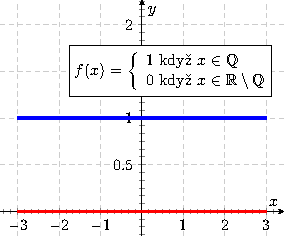
\includegraphics[width=0.5\linewidth]{mai_fig005.pdf}
        \caption{Pokus o zobrazení Dirichletovy funkce: \uv{dvě rovnoběžné přímky $y=0$ a $y=1$ s 
        nekonečným množstvím mezer}}
        \label{mai:fig005}
      \end{figure}      
      Z předchozí kapitoly také víme, že zadat funkci znamená udat její definiční obor a 
      \uv{zobrazovací předpis}, tj pravidlo (formulované slovně či v používaném matematickém 
      jazyku), podle něhož můžeme jednoznačným způsobem rozhodnout, jaká funkční hodnota odpovídá 
      libovolně zvolenému číslu z definičního oboru. Definičním oborem bývá často interval nebo 
      sjednocení intervalů. Není-li definiční obor udán, rozumíme jím množinu všech reálných čísel, 
      pro něž je příslušný předpis definován. Tuto množinu nazýváme \textbf{přirozeným} (též 
      maximálním) definičním oborem funkce. Je to tzv. \emph{existenční obor} výrazu, jímž je 
      funkce definována \cite[s.~84]{Brabec1989}.
      
      Například funkce $f: \realset\rightarrow\realset,\ f(x)=x^2$, můžeme vyjádřit bez udání 
      definičního oboru $\realset$ vztahem 
      \begin{equation*}
        f: y=x^2,
      \end{equation*}
      neboť předpis $y=x^2$ má smysl pro každé reálné číslo $x$. Avšak u funkce $g:\langle0, 
      1\rangle\rightarrow\realset,\ g(x)=x^2,$ je nutné v zápisu funkce definiční obor $\langle0, 
      1\rangle$ 
      uvést, píšeme tedy   
      \begin{equation*}
        g: y=x^2, \quad x\in\langle0,1\rangle.
      \end{equation*}
       
      %-------------------------------------
        % !TeX spellcheck = cs_CZ
\wikitextrule
\begin{example}\label{MAI:exam018} 
  Vzorcem $f(x)=\sqrt{1-x}$ je dána funkce, jejímž přirozeným oborem je interval 
  $(-\infty,1\rangle$ (uvažme, že výraz $\sqrt{1-x}$ je definován v reálném oboru, je-li 
  $1-x\geq0$). Graf této funkce je část paraboly, jejíž osou je osa $x$, viz obr. 
  \ref{mai:fig006}.
  
  {\centering
   \captionsetup{type=figure}
%  % !TeX spellcheck = cs_CZ
% mai_fig006.tex

\documentclass[11pt]{standalone}
\usepackage{xltxtra}
\usepackage[usenames,x11names]{xcolor}
\usepackage{tikz}
\usepackage{pgfplots}
  \pgfplotsset{compat=newest}
\usepackage{amsmath}


\begin{document}
  \begin{tikzpicture}[thick,scale=0.7, every node/.style={transform shape}]
    \begin{axis}[
      xmin = -3, xmax = 1.5, ymin = 0, ymax = 3,  % osy
      domain = -3:1,
      restrict y to domain=0:4,
      grid = major,   % both
      grid style={line width=.1pt, draw=gray!20},
      major grid style={dashed, line width=.2pt, draw=gray!40},
      minor tick num=5,
      clip = true,
      clip mode=individual,
      axis x line = middle,
      axis y line = middle,
      xlabel={\(x\)},
    %  xlabel style={at=(current axis.right of origin), anchor=west},
      ylabel={\(y\)},
    %  ylabel style={at=(current axis.above origin), anchor=south},
      enlarge y limits={rel=0.13},
      enlarge x limits={rel=0.07},
    ]
    
     \addplot[color=Gold3, samples=200, smooth, ultra thick, unbounded coords=jump, no markers] 
        gnuplot{sqrt(1-x)};  
    \end{axis}
  \end{tikzpicture}
\end{document} 
   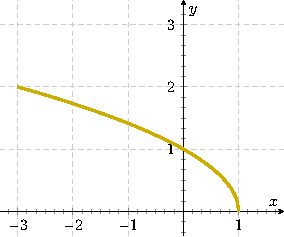
\includegraphics[width=0.5\linewidth]{mai_fig006.pdf}
   \captionof{figure}{{Graf funkce $y=\sqrt{1-x}$ je část paraboly, jejíž hlavní osou je osa $x$}}
   \label{mai:fig006}
   \par}

\end{example}
      %-------------------------------------
      
      %-------------------------------------
        % !TeX spellcheck = cs_CZ
\begin{mdframed}[style=mdexam]
  \begin{example}\label{MAI:exam019} 
    Funkce je dána vzorcem 
    \begin{equation*}
      f(x):y=\abs{x}.
    \end{equation*} 
    Přirozeným definičním oborem této funkce je množina $\realset$. Táž funkce může být dána i 
    vzorcem
    \begin{equation*}
      f(x):y=\sqrt{x^2},
    \end{equation*}    
    nebo dvěma rovnicemi
    \begin{equation*}
      f(x):y=
        \begin{cases}
             x & \text{je-li} x \geq 0. \\
            -x & \text{je-li} x < 0,
        \end{cases}                 
    \end{equation*}  
    což je zřejmé, uvědomíme-li si jak je definována absolutní hodnota. Graf funkce je na obr. 
    \ref{mai:fig007}.
    
    {\centering
    \captionsetup{type=figure}
  %  % !TeX spellcheck = cs_CZ
% mai_fig007.tex

\documentclass[11pt]{standalone}
\usepackage{xltxtra}
\usepackage[usenames,x11names]{xcolor}
\usepackage{tikz}
\usepackage{pgfplots}
  \pgfplotsset{compat=newest}
\usepackage{amsmath}

\begin{document}
  \begin{tikzpicture}[thick,scale=0.7, every node/.style={transform shape}]
    \begin{axis}[
      xmin = -3, xmax = 3, ymin = 0, ymax = 3,  % osy
      domain = -3:3,
      restrict y to domain=0:3,
      grid = major,   % both
      grid style={line width=.1pt, draw=gray!20},
      major grid style={dashed, line width=.2pt, draw=gray!40},
      minor tick num=5,
      clip = true,
      clip mode=individual,
      axis x line = middle,
      axis y line = middle,
      xlabel={\(x\)},
    %  xlabel style={at=(current axis.right of origin), anchor=west},
      ylabel={\(y\)},
    %  ylabel style={at=(current axis.above origin), anchor=south},
      enlarge y limits={rel=0.13},
      enlarge x limits={rel=0.07},
    ]
    
     \addplot[color=Gold3, samples=200, smooth, ultra thick, unbounded coords=jump, no markers] 
        gnuplot{abs(x)};  
    \end{axis}
  \end{tikzpicture} 
\end{document}
    \luafigure[0.9]{mai_fig007.pdf}
    \captionof{figure}{Graf funkce $y=\abs{x}$}
    \label{mai:fig007}
    \par}
  \end{example}
\end{mdframed}
      %-------------------------------------
      
      Funkce může být analyticky zadána i jinak než vzorcem $y=f(x)$. Časté je \textbf{parametrické 
      vyjadřování}, tj. vyjádření dvojicí rovnic 
      \begin{equation}\label{mai:eq027}
        x=\varphi(t),\ y=\psi(t),\ t\in J,
      \end{equation}
      kde $\varphi, \psi$ jsou funkce definované na množině $J$ ($\ J$ bývá obvykle interval). 
      Proměnná $t$ se nazývá \emph{parametr}: má zde pomocný význam. Zajímá nás totiž vztah mezi 
      $x$ a $y$. Rovnice \ref{mai:eq027} definuje relaci 
      $f\subset\realset\times\realset=\realset^2$:
      \begin{equation*}
        f = \{(x,y)\in\realset^2; \text{ existuje } t\in J \text{ tak, že } x=\varphi(t),\ y=\psi(t)\}.
      \end{equation*}      
      Tato relace může být za \emph{určitých podmínek jednoznačná} tj. je funkcí z $\realset$ do 
      $\realset$. V tomto případě říkáme, že funkce $f$ je \emph{definována parametricky rovnicemi 
      \ref{mai:eq027}}
      
      %-------------------------------------
        % !TeX spellcheck = cs_CZ
\begin{mdframed}[style=mdexam]
  \begin{example}\label{mai:exam020} 
    Rovnice $x=\cos t,\ y=\sin t\quad t\in\langle0,\pi\rangle$, definují parametricky funkci 
    \begin{equation}
      f: y= \sqrt{1-x^2}, \quad x\in\langle-1,1\rangle,
    \end{equation}
    jejíž grafem je polokružnice, ležící v horní polorovině $\{(x,y)\in\realset^2, y\geq0\}$.
    
    {\centering
    \captionsetup{type=figure}
  %   % !TeX spellcheck = cs_CZ
%Graf funkce \(y=\sqrt{1-x^2}\) je polokružnice

\documentclass[11pt]{standalone}
\usepackage{xltxtra}
\usepackage[usenames,x11names]{xcolor}
\usepackage{tikz}
\usepackage{pgfplots}
  \pgfplotsset{compat=newest}
\usepackage{amsmath}

\begin{document}
  \begin{tikzpicture}[thick,scale=0.7, every node/.style={transform shape}]
    \begin{axis}[
      xmin = -1.2, xmax = 1.2, ymin = 0, ymax = 1.3,  % osy
      domain = -1:1,
      restrict y to domain=0:1,
      unit vector ratio=1 1 1,  % axis equal
      grid = major,   % both
      grid style={line width=.1pt, draw=gray!20},
      major grid style={dashed, line width=.2pt, draw=gray!40},
      minor tick num=5,
      clip = true,
      clip mode=individual,
      axis x line = middle,
      axis y line = middle,
      xlabel={\(x\)}, ylabel={\(y\)},
      enlarge y limits={rel=0.07},
      enlarge x limits={rel=0.07},
    ]
    
      \addplot[color=Gold3, samples=200, smooth, ultra thick, unbounded coords=jump, no markers] 
         gnuplot{sqrt(1-x^2)};  
    \end{axis}
  \end{tikzpicture} 
\end{document}
    \luafigure[0.9]{mai_fig008.pdf}
    \captionof{figure}{Graf funkce \(y=\sqrt{1-x^2}\) je polokružnice}
    \label{mai:fig008}
    \par}
  \end{example}
\end{mdframed}
      %-------------------------------------
      
      Blíže se parametrickým zadáním funkce budeme zabývat v kapitole \ref{chap:Apl_dif_poc}
      (Aplikace diferenciálního počtu).
      
      Funkce může být někdy zadána též rovnicí tvaru 
      \begin{equation}\label{mai:eq028}
        F(x,y) = 0.
      \end{equation}
      Přitom $F$ je funkce dvou proměnných, tj. zobrazení z $\realset^2\rightarrow\realset$. Kromě 
      rovnice \ref{mai:eq028} může být dána ještě podmínka, aby bod $(x,y)$ patřil k některé 
      množině $M\subset\realset^2$. Rovnicí \ref{mai:eq028} je definována opět jakási relace 
      $f\subset\realset\times\realset$,
      \begin{equation}
        f = \{(x,y)\in\realset^2,\quad F(x,y)=0 \}
      \end{equation}
      (případně $f = \{(x,y)\in\realset^2,\ F(x,y)=0,\ (x,y)\in M \}$), zajímá nás, kdy tato relace 
      je funkcí z $\realset$ do $\realset$. Říkáme pak, že funkce $f$ je dána \textbf{implicitně} 
      uvedenou rovnicí \ref{mai:eq028} (příp. rovnicí \ref{mai:eq028} a podmínkou $(x,y)\in 
      M$). Naproti tomu zadání funkce ve tvaru $y=f(x)$ nazýváme \textbf{explicitním}.

      %-------------------------------------
        % !TeX spellcheck = cs_CZ
\begin{mdframed}[style=mdexam]
  \begin{example}\label{MAI:exam022}\todo[inline]{Nedokončený příklad}
    \begin{itemize}
    \item[]
    \item  Rovnicí $x+2y-3=0$ je implicitně definována funkce  
          $f:y=-\dfrac{1}{2}x+\dfrac{3}{2}$.
    \item  Rovnicí $x^2+y^2=1$ a podmínkou $y\geq0$ je definována implicitní funkce z příkladu 
          \ref{MAI:exam020}. Relace $\{(x,y)\in\realset^2;\ x^2+y^2=1\}$ není ovšem jednoznačná, 
          každé hodnotě $x\in(-1,1)$ odpovídají dvě hodnoty $y: y_1=\sqrt{1-x^2}$, $y: y_2 = 
          -\sqrt{1-x^2}$. Podmínkou $y\geq0$ druhou hodnotu vylučujeme. Místo podmínky $y\geq0$ 
          bychom mohli uvést i jiné podmínky, aby rovnice $x^2+y^2=1$ určovala implicitní funkci.   
    \end{itemize}
  \end{example}
\end{mdframed}
      %-------------------------------------
      
      Vyšetřování podmínek, při nichž rovnice $F(x,y)=0$ je definována funkce $f$, se obvykle 
      provádí metodami matematické analýzy funkce více proměnných. 
          
    %---------------------------------------------------------------------------------------------- 
    \subsection{Vlastnosti funkcí}\label{MA1:subsec_vlastnosti_funkce}
      \subsubsection{Omezená funkce}
        \begin{definition}\label{MA1:def_lim01}
          Funkci $f$ nazýváme shora (zdola) omezenou na množině $A\subset D(f)$, je-li shora 
          (zdola) omezená množina funkčních hodnot $f(A)$. Je-li funkce $f$ omezená shora i zdola 
          na množině $A$, pak ji nazýváme omezenou na množině $A$. Je-li $A=D(f)$, nazýváme funkci 
          omezenou. Viz kniha \cite[s.~87]{Brabec1989}       
        \end{definition}
        Funkce \(f\) je omezená na množině \(A\), právě když existuje číslo \(K>0\) tak, že platí
        \begin{align*}
         |f(x)|      &\leq K \qquad \text{pro každé } x\in A   \\ 
         \shortintertext{neboli}
         -K\leq f(x) &\leq K \qquad \text{pro každé } x\in A. 
        \end{align*}

        %-------------------------------------
          % !TeX spellcheck = cs_CZ
\wikitextrule
\begin{example}\label{MAI:exam023}
  Funkce $f:y=\dfrac{1}{x^2+1}$ je omezená. Platí totiž 
  \begin{equation*}
    \left|\frac{1}{x^2+1}\right|=\frac{1}{x^2+1}\leq1 \qquad \text{pro všechna }x\in\realset.
  \end{equation*}
  Zdola je tato funkce omezena dokonce číslem $0$.  
\end{example}
        %-------------------------------------

        \begin{itemize}\addtolength{\itemsep}{-0.5\baselineskip}
          \item Je-li funkce $f$ shora omezená na množině $A$, existuje konečné \emph{supremum}     
                $\sup f(A)$. Toto číslo nazýváme \emph{supremem funkce $f$ na množině $A$} a 
                označujeme je též $\sup_{x\in A}f(A)$ nebo $\sup\{f(x), x\in A\}$.
          \item Je-li funkce $f$ zdola omezená na množině $A$, existuje konečné \emph{infimum} 
                $\inf(A)$, které nazýváme \emph{infimum funkce $f$ na množině $A$} a označujeme je 
                též $\inf_{x\in A}f(A)$ nebo $\inf\{f(x), x\in A\}$. 
          \item Není-li funkce $f$ shora (zdola) omezená na množině $A$, pak je ovšem $\sup_{x\in A}
                f(x)=+\infty$ ($\sup_{x\in A} f(x)=-\infty$).
          \item Má-li množina $f(A)$ největší (nejmenší) prvek, pak toto číslo nazýváme největší 
                (nejmenší hodnotou funkce $f$  na množině $A$ (je-li $A = f(f)$, též absolutním 
                maximem, resp. absolutním minimem funkce $f$) a značíme je $\max_{x\in A} f(x)$ 
                ($\min_{x\in A} f(x)$). V tomto případě existuje takové číslo $x_0\in A$, že 
                $f(x_0)=\max_{x\in A}f(x)$ ($f(x_0)=\min_{x\in A}f(x)$). Pro všechna $x\in A$ tedy 
                platí $f(x)\leq f(x_0)$ ($f(x)\geq f(x_0)$). Je zřejmé, že největší (nejmenší) 
                hodnota funkce $f$ na množině $A$, pokud existuje je současně supremem (infimem) 
                funkce $f$ na $A$.
        \end{itemize}

      %-------------------------------------
        % !TeX spellcheck = cs_CZ
\wikitextrule
\begin{example}\label{MAI:exam021} 
  Pro funkci z příkladu \ref{MAI:exam023} platí:
  \begin{align*}
    \sup_{x\in\realset}&=\frac{1}{x^2+1}=\max_{x\in\realset}=\frac{1}{x^2+1}=1;   \\
    \inf_{x\in\realset}&=\frac{1}{x^2+1}=0,
  \end{align*}
  tato funkce však nenabývá v definičním oboru $\realset$ nejmenší hodnoty, neboť je stále 
  $\dfrac{1}{x^2+1}>0$. To, že infimum je $0$, dokážeme takto: Zvolíme-li libovolně 
  $\varepsilon>0$, pak snadno zjistíme, že existuje $x$, pro něž 
  $\dfrac{1}{x^2+1}<\varepsilon$:
  \begin{align*}
    1                  &< \varepsilon(x^2+1) \\
    \frac{1}{\epsilon} &< x^2+1 \Rightarrow \sqrt{\frac{1}{\epsilon}-1} < x
  \end{align*} 
  
  {\centering
   \captionsetup{type=figure}
%   % !TeX spellcheck = cs_CZ
%Graf funkce $f(x):y=\dfrac{1}{1+x^2}$

\documentclass[11pt]{standalone}
\usepackage{xltxtra}
\usepackage[usenames,x11names]{xcolor}
\usepackage{tikz}
\usepackage{pgfplots}
  \pgfplotsset{compat=newest}
\usepackage{amsmath}

\begin{document}
  \begin{tikzpicture}[thick,scale=0.7, every node/.style={transform shape}]
    \begin{axis}[
      xmin = -4.2, xmax = 4.5, ymin = 0, ymax = 1.3,  % osy
      domain = -4:4,
      restrict y to domain=0:1,
  %    unit vector ratio=1 1 1,  % axis equal
      grid = major,   % both
      grid style={line width=.1pt, draw=gray!20},
      major grid style={dashed, line width=.2pt, draw=gray!40},
      minor tick num=5,
      clip = true,
      clip mode=individual,
  %    /pgfplots/xtick={-2,-1,1,2}, % make steps of length 0.2
      axis x line = middle,
      axis y line = middle,
      xlabel={\(x\)}, ylabel={\(y\)},
      enlarge y limits={rel=0.07},
      enlarge x limits={rel=0.07},
    ]
    
      \addplot[color=Gold3, samples=200, smooth, ultra thick, unbounded coords=jump, no markers] 
         gnuplot{1/sqrt(1+x^2)};  
    \end{axis}
  \end{tikzpicture}
\end{document} 
   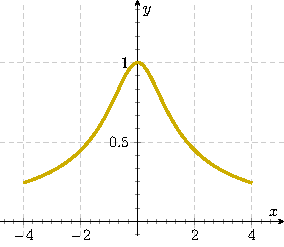
\includegraphics[width=0.5\linewidth]{mai_fig009.pdf}
   \captionof{figure}{Graf funkce $f(x):y=\dfrac{1}{1+x^2}$}
   \label{mai_fig009}
  \par}
  
  Neexistuje tedy kladné číslo, jež by bylo dolní mezí množiny funkčních hodnot, takže infimum je 
  $0$. Graf funkce $f$ je na obr. \ref{mai_fig009}.
\end{example}
      %-------------------------------------
       
      \subsubsection{Monotonní funkce}
        \begin{definition}\label{MA1:def_lim02}
          Funkci $f$ nazýváme \textbf{rostoucí (klesající)} na množině $A\subset D(f)$, jestliže 
          pro každé dva body $x_1, x_2\in A,\ x_1<x_2$, platí $f(x_1)<f(x_2)$ ($f(x_1)>f(x_2)$). 
          Funkci $f$ nazýváme \textbf{neklesající (nerostoucí)} na množině $A\subset D(f)$, 
          jestliže pro každé dvě body $x_1, x_2\in A,x_1<x_2$, platí $f(x_1)\leq f(x_2)$ 
          ($f(x_1)\geq f(x_2)$). Rostoucí a klesající funkce (na množině $A$) se nazývají 
          \textbf{ryze monotónní} (na množině $A$), neklesající a nerostoucí funkce (na množině 
          $A$) se nazývají monotónní (na množině $A$).    
        \end{definition}
            
        Z definice je zřejmé, že každá rostoucí funkce je zároveň neklesající a každá klesající 
        funkce je zároveň nerostoucí. Ryze monotónní funkce tvoří tedy podmnožinu množiny 
        monotónních funkcí. 
           
        \begin{example}
          Funkce $y=2x+1$ je \textbf{rostoucí} na intervalu $(-\infty, \infty)$. Platí totiž: $x_1<x_2\Rightarrow 2x_1<2x_2\Rightarrow2x_1+1<2x_2+1$.
        \end{example}
        \begin{example}
          Funkce y=[x] je \textbf{neklesající} na intervalu $(-\infty, \infty)$ (viz příklad **). 
        \end{example}
        \begin{example}
          Heavisideova funkce (viz příklad **) je \textbf{neklesající} na intervalu $(-\infty, \infty)$ (viz příklad **). 
        \end{example}       
        \begin{example}
          Funkce $y=|x|$ je \textbf{klesající} na intervalu $(-\infty, 0\rangle$ a rostoucí na intervalu $\langle0, \infty)$. 
        \end{example}  
            
        \begin{definition}\label{MA1:def_lim03}
          Funkci $f$ nazýváme \textbf{konstantní} na množině $A$, jestliže pro každé dva body $x_1, 
          x_2\in A$, platí $f(x_1)=f(x_2)$. V tom případě existuje reálné číslo $k$ takové, že pro 
          každé $x\in A$ je $f(x)=k$. Je-li $k=0$, mluvíme o nulové funkci na množině $A$. 
        \end{definition} 
          
        Výrok \uv{funkce $f$ je konstantní na množině $A$} zapisujeme též $f(x)=\text{konst na }A$. 
        Funkci konstantní na $\realset$ budeme stručně nazývat \textbf{konstantní funkcí} nebo 
        krátce \textbf{konstantou}. Z textu bude obvykle patrno, interpretujeme-li symbol $k$ jako 
        reálné číslo nebo jako konstantní funkci. Je zřejmé, že konstantní funkce na množině $A$ je 
        zároveň neklesající i nerostoucí na množině $A$. Toto tvrzení se dá obrátit. Lze snadno 
        dokázat i tuto větu:        
        \begin{lemma}\label{MA1:lem_lim01}
          Funkce $f$ je \textbf{rostoucí} na množině $A$, právě když je neklesající na množině $A$ a na žádné dvoubodové podmnožině $B\subset A$ není konstantní. 
        \end{lemma}
        Obdobná tvrzení platí i pro klesající funkce. 
               
      \subsubsection{Sudé a liché funkce}
        \begin{definition}\label{MA1:def_lim04}
          Funkce $f$ se nazývá \textbf{sudá} jestliže pro každé $x\in D(f)$ je též $-x\in D(f)$  a 
          platí $f(x)=f(-x)$.
          Funkce $f$ se nazývá \textbf{lichá} jestliže pro každé $x\in D(f)$ je též $-x\in D(f)$  a 
          platí $f(-x)=-f(x)$. 
        \end{definition}
        Graf sudé funkce je souměrný podle osy $y$ (osy funkčních hodnot), graf liché funkce je  
        souměrný podle počátku. 
 
       %-------------------------------------
         % !TeX spellcheck = cs_CZ
\wikitextrule
\begin{example}\label{MAI:exam024} 
  Funkce $f:\,y=x^2$ je sudá, funkce $g:\,y=x^3$ je lichá.
  
  {\centering
   \begin{tabular}{cc}
     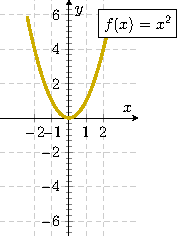
\includegraphics[width=0.5\linewidth]{mai_fig010.pdf}              &
     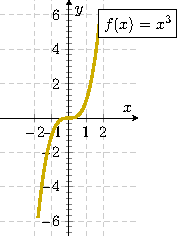
\includegraphics[width=0.5\linewidth]{mai_fig011.pdf}             \\
  \end{tabular}
  \captionsetup{type=figure}
  \captionof{figure}{Příklad sudé a liché funkce}\label{MAI:fig_002}
  \par}
\end{example}
       %-------------------------------------

        Daná funkce nemusí být ovšem ani sudá, ani lichá. Snadno se dokáže tvrzení:
        \begin{itemize}
          \item Je-li sudá funkce $f$ na množině $D(f)\cap\langle0,\infty)$ rostoucí (klesající),
                je na množině $D(f)\cap(-\infty,0\rangle$ klesající (rostoucí).
          \item Je-li lichá funkce na množině $D(f)\cap\langle0,\infty)$ rostoucí (klesající),
                je též na množině $D(f)\cap(-\infty,0\rangle$ klesající (rostoucí).                 
        \end{itemize}
      \subsubsection{Periodická funkce}

    \subsection{Operace s funkcemi. Uspořádání}
      Jak s funkcemi počítat? Definujeme základní operace s nimi — \emph{součet funkcí, součin 
      funkcí a násobení funkce reálným číslem}. Předpokládejme, že na definičním oboru 
      \(\mathcal{D}\) jsou zadány funkce \(f\) a \(g\) a reálné číslo \(\alpha\). Pak na tomtéž 
      definičním oboru lze zadat nové funkce
      \begin{align*}
        \mathcal{F} &: \mathcal{D}\ni x\,\rightarrow\,\mathcal{F}(x) = f(x)+g(x)  \in\realset   \\
        \mathcal{G} &: \mathcal{D}\ni x\,\rightarrow\,\mathcal{G}(x) = \alpha g(x)\in\realset   \\
        \mathcal{H} &: \mathcal{D}\ni x\,\rightarrow\,\mathcal{H}(x) = f(x) g(x)  \in\realset 
      \end{align*}
      Funkce \(\mathcal{F}\), \(\mathcal{G}\) a \(\mathcal{H}\) nazýváme postupně součtem funkcí 
      \(f\) a \(g\), \(\alpha\)-násobkem funkce \(f\) a součinem funkcí \(f\) a \(g\). Značíme
      \begin{equation*}
       \mathcal{F} = f + g, \qquad \mathcal{G} = \alpha f, \qquad \mathcal{H} = fg. 
      \end{equation*}
      
      Všimněme si nyní pravidel pro počítání s funkcemi zadanými na \(\mathcal{D}\) a zjistíme, 
      že se velmi podobají pravidlům pro počítání s reálnými čísly. Není divu, vždyť operace s 
      funkcemi jsou definovány prostřednictvím funkčních hodnot, a těmi jsou reálná čísla. Některé 
      důležité odlišnosti však přece jen najdeme. Napřed ale pravidla:
      
      \begin{itemize}\addtolength{\itemsep}{-0.5\baselineskip}
        \item komutativní zákon pro součet funkcí
          \begin{equation}\label{mai:eq012}
            f(x) + g(x) = g(x) + f(x)
          \end{equation}
        \item asociativní zákon pro součet funkcí  
          \begin{equation}\label{mai:eq013}
            (f(x) + g(x)) + h(x) = f(x) + (g(x) + h(x)
          \end{equation}
        \item existence univerzálního neutrálního  prvku \(O\) (nulová funkce \(O:\mathcal{D}\ni x 
          \rightarrow O(x)=0\))
          \begin{equation}\label{mai:eq014}
            f(x) + O = O + f(x) = f(x)
          \end{equation}
        \item existence právě jednoho opačného prvku k funkci \(f\), přičemž \((-f)(x) = -f(x)\)
          \begin{equation}\label{mai:eq015}
            f(x)+(-f(x))=(-f(x))+f(x)=O
          \end{equation}
        \item asociativní zákon pro násobení číslem 
         \begin{equation}\label{mai:eq016}
            (\alpha_1\alpha_2)f(x) = \alpha_1(\alpha_2f(x))
         \end{equation}
        \item  1. distributivní zákon pro násobení číslem
          \begin{equation}\label{mai:eq017}
            \alpha(f(x)+g(x) =\alpha f(x) + \alpha g(x)
          \end{equation}\label{mai:eq018}
        \item 2. distributivní zákon pro násobení číslem 
          \begin{equation}\label{mai:eq019}
            (\alpha_1+\alpha_2)f(x) =\alpha_1f(x)+\alpha_2f(x)
          \end{equation}
        \item násobení číslem \((—1)\) dává opačný prvek
          \begin{equation}\label{mai:eq020}
            (-1)f(x)=(-f(x))
          \end{equation}
        \item komutativní zákon pro součin funkcí
          \begin{equation}\label{mai:eq021}
            f(x)g(x)=g(x)f(x)
          \end{equation}
        \item asociativní zákon pro součin funkcí 
          \begin{equation}\label{mai:eq022}
            f(x)(g(x)h(x))=(f(x)g(x))h(x)
          \end{equation}
        \item distributivní zákon zprava pro součin funkcí
          \begin{equation}\label{mai:eq023}
            (f_1(x) + f_2(x))g(x) =f_1(x)g(x) + f_2(x)g(x)
          \end{equation}
        \item distributivní zákon zleva pro součin funkcí
          \begin{equation}\label{mai:eq024}
            f(x)(g_1(x) + g_2(x))=f(x)g_1(x)+f(x)g_2(x)
          \end{equation}
        \item násobení jednotkovou funkcí \(I: \mathcal{D}\ni x \rightarrow I(x) = 1\)  
          \begin{equation}\label{mai:eq025}
           f(x)I=If(x)
          \end{equation}
        \item existence právě jedné \emph{převrácené} funkce k funkci \(f\) pro \(f(x)\neq0\quad 
              (f)^{-1}: \bar{D}\ni x\rightarrow (f)^{-1}(x)=[f(x)]^{-1}\) kde \(\bar{\mathcal{D}} 
              = \mathcal{D} - \left\{x\in \mathcal{D}\,|\,f(x)=0\right\}\)
          \begin{equation}
            f(x)(f(x))^{-1}=(f(x))^{-1}f(x) = I
          \end{equation}
      \end{itemize}
      Všimněme si, že funkce \((f)^{-1}\) existuje obecně na užším definičním oboru 
      \(\bar{\mathcal{D}}\), než na kterém je definována funkce \(f\). Je totiž třeba vyloučit 
      všechny hodnoty \(x\), pro které \(f(x) = 0\) (zákaz dělení nulou). K funkci \(O\) tedy 
      převrácená funkce neexistuje vůbec!
      
      Existence opačné a převrácené funkce k \(f\) umožňuje definovat \emph{rozdíl} a \emph{podíl} 
      funkcí \(f-g=f+(-g)\) a \(\dfrac{f}{g}=f(g)^{-1}\), tj.
      \begin{align*}
        f-g         &: \mathcal{D}\ni x\,\rightarrow\, (f-g)(x)=f(x)+(-g)(x)= f(x)-g(x), \\
        \frac{f}{g} &: \bar{D}\ni x\,\rightarrow\, 
                       \left(\frac{f}{g}\right)(x) = f(g)^{-1}(x) = \frac{f(x)}{g(x)}, 
      \end{align*}
      kde \(\bar{D}=D-\left\{x\in D\,|\,g(x)=0 \right\}\) 
      
      \begin{note}
        Pamatujme si označení převrácené funkce jako \((f)^{-1}\), v němž je zápis symbolu \(f\) do 
        závorky podstatný. Jde o něco jiného než znamená symbol \(f^{-1}\) bez závorky, který 
        rezervujeme pro inverzní funkci v dalším výkladu.
      \end{note}
      \begin{note}
        Porovnáme-li nyní vlastnosti operací s funkcemi a pravidla pro počítání s reálným čísly, 
        komplexními čísly, maticemi a vektory, můžeme konstatovat, že množina funkcí s operací 
        sčítání funkcí a násobení funkce číslem je \textbf{vektorovým prostorem}. To je vlastnost, 
        která je s případem čísel, matic a vektorů společná. Vektorový prostor funkcí se však od 
        zmiňovaných vektorových prostorů výrazně liší svou dimenzí (rozměrem). Intuitivně dobře 
        chápeme, co znamená jednorozměrný, dvojrozměrný a trojrozměrný prostor (například 
        \(\realset^1\), \(\realset^2\), \(\realset^3\)). V odstav 1.4 jsme dokonce pracovali v 
        n-rozměrném vektorovém prostoru. Dimenze vektorového prostoru může být i nekonečná — třeba 
        zrovna u funkcí. Obecně jde o pojem poměrně obtížný a budeme se jím důkladně zabývat až v 
        kapitolách věnovaných algebře \cite[s.~58]{Musilova2009MA1}.
      \end{note}
      
      Operace s funkcemi jsme definovali a prodiskutovali pro případ, kdy definiční obory funkcí, 
      vstupujících do operace byly stejné. Co když tomu tak nebude? Znamená to, že pak nemůžeme 
      funkce sčítat, násobit, apod.? Předpokládejme, že definičním oborem funkce \(f\) je množina 
      \(\mathcal{D}_f\) definičním oborem funkce \(g\) množina \(D_g\). Pokud jsou tyto obory 
      disjunktní, tj. \(\mathcal{D}_f \cap \mathcal{D}_g = 0\), můžeme utvořit pouze 
      \(\alpha\)-násobek funkce \(f\) či \(g\). Sčítat ani násobit funkce \(f\) a \(g\) nemůžeme 
      neboť hodnota \(f(x) + g(x)\) ani \(f(x)g(x)\) neexistuje pro žádné \(x\). Pokud je průnik 
      \(D=d_f\cap D_g\) oborů \(\mathcal{D}_f\) a \(\mathcal{D}_g\) neprázdný, stává se definičním 
      oborem funkcí \(f+g\) a \(fg\). Platí stejná pravidla jako v předchozí tabulce, pouze s 
      omezením na obor \(\mathcal{D}_f\).
    
    \subsection{Skládání a inverze funkcí}
      \emph{Skládání} neboli kompozici funkcí si lze snadno představit opět pomocí „černých 
      skříněk“ (obr. \ref{mai:fig012}): Do první skřínky představující předpis \(g\), \emph{vnitřní 
      složku} složené funkce, vstupuje
      \begin{figure}[ht!] %\ref{mai:fig012}
        \centering
%        % !TeX spellcheck = cs_CZ
% exam017.tex

\documentclass[11pt]{standalone}
\usepackage{xltxtra}
\usepackage[usenames,x11names]{xcolor}
\usepackage{tikz}
\usepackage{pgfplots}
  \pgfplotsset{compat=newest}
\usepackage{amsmath}
\usepackage{amsfonts}          % \mathbb{R}
  \newcommand{\realset}{\mathbb{R}}

\begin{document}
  \begin{tikzpicture}[fill=black!20]
  %  \draw[help lines] (-1,-2) grid (6,3);
    \path (0,0) node(a) [ ] {\(\mathcal{D}_g\)}
    (2,0) node(b) [rectangle,rotate=0,draw,fill] 
      {\(\begin{array}{c} \text{funkce} \\ g  \end{array}\)}
    (4.5,0) node(c) [rectangle,rotate=0,draw,fill] 
      {\(\begin{array}{c} \text{funkce} \\ f  \end{array}\)}
    (7,0) node(d) [ ] {\(\realset\)};
    \draw[thick,->] (a.east) -- (b);
    \draw[thick,->] (b.east) -- (c);
    \draw[thick,->] (c.east) -- (d);
    \path [ ] (a.east) -- (b.west)   node [above,midway] {\(x\)};
    \path [ ] (b.east) -- (c.west)   node [above,midway] {\(g(x)\)};
    \path [ ] (c.east) -- (d.west)   node [above,midway] {\(f[g(x)]\)};
  \end{tikzpicture}
\end{document}
        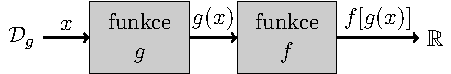
\includegraphics[width=0.45\linewidth]{mai_fig012.pdf}
        \caption{Skládání funkcí \cite[s.~59]{Musilova2009MA1}}
        \label{mai:fig012}
      \end{figure}
      hodnota \(x\) z definičního oboru \(\mathcal{D}_g\) funkce \(g\). Výstupem je číslo \(u = 
      g(x)\), funkční hodnota vnitřní složky v bodě \(x\). Toto číslo smí vstoupit do skříňky 
      představující předpis \(f\), \emph{vnější složku} složené funkce, právě tehdy, je-li prvkem 
      jejího definičního oboru \(\mathcal{D}_f\). V takovém případě najdeme na výstupu ze skříňky 
      \(f\) hodnotu \(y = f(u) = f[g(x)]\). (Jestliže \(g(x)\notin\mathcal{D}_f\), není výstup ze 
      skříňky \(f\) definován.) Vzniká nový předpis \(F\), kterým se některým bodům definičního 
      oboru \(\mathcal{D}_g\), ne všem, ale pouze těm, pro něž \(g(x)\in\mathcal{D}_f\), 
      přiřazují hodnoty \(f[g(x)]\). Definujme nyní složenou funkci přesněji: Předpokládejme, že 
      jsou zadány funkce
      \begin{align*}
        g  &: \mathcal{D}_g\ni x\,\rightarrow\, g(x) = u\in\realset, \\
        f  &: \mathcal{D}_f\ni u\,\rightarrow\, f(u) = y\in\realset. \\
        \shortintertext{označme}
        \mathcal{D} &= \{x|x\in\mathcal{D}_g \text{ a současně } g(x)\in\mathcal{D}_f\}.
      \end{align*}
      Pokud \(\mathcal{D} = \emptyset\), lze definovat funkci
      \begin{equation*}
        F: \mathcal{D}\ni x\rightarrow y = F(x) = f[g(x)]\in\realset, 
           \text{ značíme } F = f \circ g.
      \end{equation*}
      \(F\) se nazývá \emph{složením} neboli \emph{kompozicí} funkcí \(g\) a \(f\). Zápis \(f\circ 
      g\) čteme často také jako \emph{„f po g“}. Skládat lze i větší počet funkcí.

       %-------------------------------------
         % !TeX spellcheck = cs_CZ
\begin{mdframed}[style=mdexam]
  \begin{example}\label{MAI:exam025}
    Uvažme funkci z příkladu \ref{vol02:fyz:fey_exam017}. 
    
    {\centering
    \captionsetup{type=figure}
  %   % !TeX spellcheck = cs_CZ
\documentclass[11pt]{standalone}
\usepackage{xltxtra}
\usepackage[usenames,x11names]{xcolor}
\usepackage{tikz}
\usepackage{pgfplots}
  \pgfplotsset{compat=newest}
\usepackage{amsmath}

\begin{document}
  \begin{tikzpicture}[thick,scale=0.7, every node/.style={transform shape}]
    \begin{axis}[
      xmin = -5, xmax = 5, ymin = -10, ymax = 1.5,
   %   domain = -0.999999:0.999999,
      restrict y to domain=-30:1.5,
      unit vector ratio=1 1 1,  % axis equal
      grid = both,   % both, major
      grid style={line width=.1pt, draw=gray!20},
      major grid style={dashed, line width=.2pt, draw=gray!40},
      minor tick num=4,
      clip = true,
      clip mode=individual,
      axis x line = middle,
      axis y line = middle,
      xlabel={$x$},
    %  xlabel style={at=(current axis.right of origin), anchor=west},
      ylabel={$u,w,y$},
    %  ylabel style={at=(current axis.above origin), anchor=south},
      enlarge y limits={rel=0.13},
      enlarge x limits={rel=0.07},
    ]
    
      \addplot[color=Gold3, samples=1000, smooth, ultra thick, unbounded coords=jump, no markers, 
               domain = -0.999999:0.999999] 
        gnuplot{log10(sqrt(1-x^2))/log10(2)};  
        
     \addplot[color=green, samples=200, smooth, ultra thick, unbounded coords=jump, no markers, 
     domain = -3.3:3.3] 
        gnuplot{1-x^2};
        
     \addplot[color=blue, samples=200, smooth, ultra thick, unbounded coords=jump, no markers, 
     domain = -1:1] 
        gnuplot{sqrt(1-x^2)};  
    \end{axis}
  \end{tikzpicture}
\end{document}
    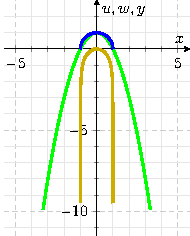
\includegraphics[width=0.6\linewidth]{mai_fig013.pdf}
    \captionof{figure}{K příkladu \ref{MAI:exam025} \(y=\log_2{(\sqrt{1-x^2})}\) 
    \cite[s.~57]{Musilova2009MA1}
    \label{mai:fig013}}
    \par}
    
    Ukážeme, jak tato funkce vzniká postupně složením tří funkcí a jak při tom dochází k postupnému 
    omezování definičního oboru. Písmeny \(\mathcal{D}\) a \(H\) s příslušným indexem budeme značit 
    definiční obory a obory hodnot jednotlivých funkcí.
    \begin{gather*}
      \begin{align*}
        g&:  \realset =\mathcal{D}_g\ni x\rightarrow u=g(x) = 1- x^2  \in\mathcal{H}_g=(-\infty,1], \\
        h&: [0,\infty)=\mathcal{D}_h\ni u\rightarrow w=h(u) = \sqrt{u}\in\mathcal{H}_h=[0,\infty),  \\
       \shortintertext{\(\mathcal{D}_h\cap\mathcal{H}_g = [0,1]\Rightarrow\mathcal{D}_{h\circ g}=[-1,1], 
                       \mathcal{H}_{h\circ g} = [0,1],\)}                                    \\
       f&:(0,\infty)=\mathcal{D}_f\ni w \rightarrow y=f(w)=\log_2w\in\mathcal{H}_f=\realset  \\
       \shortintertext{\(\mathcal{H}_{h\circ g}\cap\mathcal{D}_f = (0,1] 
                       \Rightarrow\mathcal{D}_F=(-1,1),\mathcal{H}_F=(-\infty,0].\)} 
      \end{align*}
    \end{gather*}
    Je tedy
    \begin{gather*}
      \begin{align*}
        F:\mathcal{D}_F\ni x\rightarrow 
        y&=F(x)=(f\circ(h\circ g))(x) = f{h[g(x)]}          \\
        &= \log_2\sqrt{1-x^2}\in(-\infty,0].
      \end{align*}
    \end{gather*}
    Názorněji než tento zápis ukazuje situaci obrázek \ref{mai:fig013}.
  \end{example}
\end{mdframed}
       %-------------------------------------
      
      Může vzniknout otázka, jak rozpoznáme vnitřní a vnější složku složené funkce. Rozlišit 
      vnitřní a vnější složku třeba u funkcí \(\cos(x^2)\) a \((cos x)^2\) není problém. Hned také 
      vidíme, že obecně \(f\circ g\neq g\circ f\), i když by definiční obory funkcí na pravé i levé 
      straně měly neprázdný průnik. Jsou však i případy na první pohled méně zřetelné, jak ukazuje 
      následující příklad.
      
      %-------------------------------------
        % !TeX spellcheck = cs_CZ
\begin{mdframed}[style=mdexam]
  \begin{example}\label{mai:exam026}
    (Určení vnitřní a vnější složky) Uveďme příklad dvou funkcí \(F(x)=\sqrt{x^2}\) a \(G(x) =
    (\sqrt{x})^2\). Liší se tyto funkce, nebo jde o tutéž funkci, jen jinak zapsanou? Vidíme, že
    platí

    \begin{align*}
      \mathcal{D}_F &=\realset, F(x)=\abs{x}\forall x\in\mathcal{D}_F, \mathcal{H}_F = [0, infty),\\
      \mathcal{D}_G &=[0, \infty), G(x)=x\forall    x\in\mathcal{D}_G, \mathcal{H}_G = [0, infty).
    \end{align*}
    Funkce \(F\) a \(G\) mají různé definiční obory, ale na jejich průniku dávají stejné funkční
    hodnoty. Ani zde však obecně nelze pořadí skládání funkcí zaměňovat.
  \end{example}
\end{mdframed}
      %-------------------------------------
       
      Funkce \(F\) a \(G\) mají různé definiční obory, ale na jejich průniku dávají stejné funkční 
      hodnoty. Ani zde však obecně nelze pořadí skládání funkcí zaměňovat.
      
      Nyní se pusťme do vybudování pojmu inverzní funkce k funkci \(f\). Představme si, že funkční
      hodnota \(y = f(x)\) zadané funkce
      \begin{equation*}
        f: \mathcal{D}_f\ni x \rightarrow f(x)\in\mathcal{H}_f
      \end{equation*}
      představuje „zakódovanou“ informaci o hodnotě \(x\). Položme si otázku, zda a za jakých 
      podmínek dokážeme sestavit „černou skříňku“, na jejímž výstupu by se při vstupu obrazu \(y = 
      f(x)\) objevila hodnota \(x\). Omezení takové možnosti je názorně vidět na obrázku 
      \ref{mai:fig014}. V případě funkce \(f(x)\) lze ke všem obrazům \(y \in \mathcal{H}_f\) najít 
      vzory, v případě funkce \(g(x)\) to možné není, neboť jeden a týž obraz lze získat z několika 
      vzorů. Pro který bychom se tedy měli rozhodnout?
      
      \begin{figure}[ht!] %\ref{mai:fig014}
        \centering
%        % !TeX spellcheck = cs_CZ
% Skládání funkcí \cite[s.~61]{Musilova2009MA1}

\documentclass[11pt]{standalone}
\usepackage{xltxtra}
\usepackage[usenames,x11names]{xcolor}
\usepackage{tikz}
\usepackage{pgfplots}
  \pgfplotsset{compat=newest}
\usepackage{amsmath}
\usepackage{amsfonts}       % \mathbb{R}
  \newcommand{\realset}{\mathbb{R}}

\begin{document}
  \begin{tikzpicture}[fill=black!20]
  %  \draw[help lines] (-1,-2) grid (6,3);
    \path (0,0) node(a) [ ] {\(\mathcal{D}_f\)}
    (2,0) node(b) [rectangle,rotate=0,draw,fill] 
      {\(\begin{array}{c} \text{funkce} \\ f  \end{array}\)}
    (4.5,0) node(c) [rectangle,rotate=0,draw,fill] 
      {\(\begin{array}{c} \text{funkce} \\ f^{-1}  \end{array}\)}
    (7,0) node(d) [ ] {\(\realset\)};
    \draw[thick,->] (a.east) -- (b);
    \draw[thick,->] (b.east) -- (c);
    \draw[thick,->] (c.east) -- (d);
    \path [ ] (a.east) -- (b.west)   node [above,midway] {\(x\)};
    \path [ ] (b.east) -- (c.west)   node [above,midway] {\(f(x)\)};
    \path [ ] (c.east) -- (d.west)   node [above,midway] {\(x\)};
  \end{tikzpicture}
\end{document}
        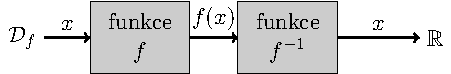
\includegraphics[width=0.45\linewidth]{mai_fig014.pdf}
        \caption{Skládání funkcí \cite[s.~61]{Musilova2009MA1}}
        \label{mai:fig014}
      \end{figure}
       Aby bylo možné vzor zpětně identifikovat na základě znalosti obrazu, je třeba, aby funkce 
       \(f\) byla \emph{prostá}, tj. aby předpis \(f\) přiřazoval každým dvěma různým vzorům \(X_1 
       \neq x_2\) dva různé obrazy \(f(x_1) \neq f(x_2)\). Často lze tohoto požadavku docílit tím, 
       že se místo funkce \(f\) s definičním oborem \(\mathcal{D}_f\) spokojíme s funkcí, která 
       vznikne omezením \emph{(restrikcí)} té původní na „menší“ definiční obor, zato však již bude 
       prostá. U funkce \(g\) na obrázku \ref{mai:fig016} by tak stačilo omezit definiční obor 
       například na množinu \(\mathcal{D}_g\). Než inverzní funkci definujeme, ukažme si způsob 
       jejího nalezení na známém příkladu.

       \begin{figure}[ht!]
         \centering  
         \begin{tabular}{cc}
           \subfloat[ ]{\label{mai:fig016a}
             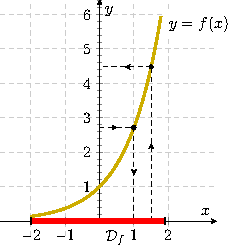
\includegraphics[width=0.45\linewidth]{mai_fig016a.pdf}}              &
           \subfloat[ ]{\label{mai:fig016b}
             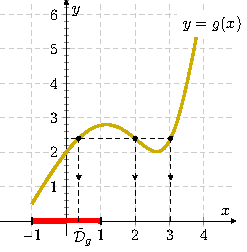
\includegraphics[width=0.45\linewidth]{mai_fig016b.pdf}}              \\
         \end{tabular}
         \caption{K pojmu inverzní funkce}
         \label{mai:fig016}
       \end{figure}
      
      %-------------------------------------
        % !TeX spellcheck = cs_CZ
\begin{mdframed}[style=mdexam]
  \begin{example}\label{MAI:exam027}
    (Nalezení inverzní funkce): Funkci 
    \begin{equation*}
      y = \log_2(\sqrt{1-x^2})
    \end{equation*}
    Jsme již z různých hledisek rozebrali v příkladech \ref{vol02:fyz:fey_exam017} a
    \ref{MAI:exam025}. Hodí se i nyní.

    {\centering
    \captionsetup{type=figure}
  %  % !TeX spellcheck = cs_CZ
% K příkladu \ref{mai:exam027} \(y=\log_2{(\sqrt{1-x^2})}

\documentclass[11pt]{standalone}
\usepackage{xltxtra}
\usepackage[usenames,x11names]{xcolor}
\usepackage{tikz}
\usepackage{pgfplots}
  \pgfplotsset{compat=newest}
\usepackage{amsmath}

\begin{document}
  \begin{tikzpicture}[thick,scale=0.7, every node/.style={transform shape}]
    \begin{axis}[
      xmin = -5, xmax = 5, ymin = -5, ymax = 1.5,
   %   domain = -0.999999:0.999999,
      restrict y to domain=-30:1.5,
      unit vector ratio=1 1 1,  % axis equal
      grid = both,   % both, major
      grid style={line width=.1pt, draw=gray!20},
      major grid style={dashed, line width=.2pt, draw=gray!40},
      minor tick num=4,
      clip = true,
      clip mode=individual,
      axis x line = middle,
      axis y line = middle,
      xlabel={\(x\)},
    %  xlabel style={at=(current axis.right of origin), anchor=west},
      ylabel={\(y\)},
    %  ylabel style={at=(current axis.above origin), anchor=south},
      enlarge y limits={rel=0.13},
      enlarge x limits={rel=0.07},
    ]
    
      \addplot[color=Gold3, samples=1000, smooth, ultra thick, unbounded coords=jump, no markers, 
               domain = 0:0.9995] 
        gnuplot{log10(sqrt(1-x^2))/log10(2)};  
        
      \addplot[color=blue, samples=200, smooth, ultra thick, unbounded coords=jump, no markers, 
               domain = -5:0] 
        gnuplot{sqrt(1-2^(2*x))};  
    \end{axis}
  \end{tikzpicture}
\end{document}
    \luafigure[0.9]{mai_fig015.pdf}
    \captionof{figure}{K příkladu \ref{MAI:exam027} \(y=\log_2{(\sqrt{1-x^2})}\) 
    \cite[s.~62]{Musilova2009MA1}
    \label{mai:fig015}}
    \par}
    
    Na obrázku \ref{mai:fig013} máme dokonce její graf, a tak vidíme, že \textbf{není} na svém 
    definičním oboru \((-1, 1)\) \textbf{prostá}. Omezme proto její definiční obor na interval 
    \(\mathcal{D} = [0, 1)\), na němž již prostá je (část grafu vpravo od osy \(y\)). Pro danou 
    hodnotu obrazu \(y \in (-\infty,0]\) můžeme již jednoznačně určit hodnotu \(x\) jednoduchou 
    úpravou:
    \begin{align*}
      y = \log_2(\sqrt{1-x^2}) &\Rightarrow \sqrt{1-x^2} = 2^y   \\
                               &\Rightarrow x^2 = 1 - 2^{2y}     \\
                               &\Rightarrow x = \sqrt{1 - 2^{2y}}
    \end{align*}
    Formální záměnou \(x \leftrightarrow y\) dostáváme inverzní funkci k funkci \(f\),
    \begin{equation*}
      y =f^{-1}(x) = \sqrt{1 - 2^{2x}}.
    \end{equation*}
    Grafy obou funkcí jsou na obrázku \ref{mai:fig015}.
  \end{example}
\end{mdframed}
      %-------------------------------------
      
      Ze způsobu konstrukce funkce \(f^{-1}\) v předchozím příkladu je vidět, že 
      \(\mathcal{D}_{f^{-1}} = \mathcal{H}_f\), \(\mathcal{H}_{f^{-1}} = \mathcal{D}_f\) a graf 
      inverzní funkce je obrazem grafu prosté funkce \(f\) při osové symetrii v rovině 
      souřadnicových os vzhledem k ose prvního a třetího kvadrantu. Nyní již definujeme inverzní 
      funkci obecně. Předpokládejme, že funkce \(f : \mathcal{D}_f\ni x \rightarrow y = f(x)\ni 
      \mathcal{H}_f\) je prostá na svém definičním oboru. Pak existuje funkce \(f^{-1}\) definovaná 
      jako
      \begin{equation}\label{mai:eq029}
        f^{-1} :\mathcal{H}_f\ni x\rightarrow y = f^{-1}(x)\in\mathcal{D}_f\Leftrightarrow x = f(y).
      \end{equation}
      Funkci \(f^{-1}\) nazýváme \textbf{inverzní funkcí k funkci} \(f\). Ještě shrneme pravidla 
      pro skládání funkcí a pro inverzní funkce:

      \begin{itemize}\addtolength{\itemsep}{-0.5\baselineskip}
        \item asociativní zákon pro skládání funkcí
          \begin{equation}\label{mai:eq030}
            f(x)\circ(h(x)\circ g(x)) = f(x)\circ h(x) \circ g(x)
          \end{equation}
        \item distributivní zákon zleva 
          \begin{equation}\label{mai:eq031}
            f(x) \circ (h(x) + g(x)) = f(x) \circ h(x) + f(x) \circ g(x)
          \end{equation}
        \item existence univerzálního neutrálního  prvku \(O\) (nulová funkce \(O:\mathcal{D}\ni x 
          \rightarrow O(x)=0\))
          \begin{equation}\label{mai:eq032}
            f(x) + O = O + f(x) = f(x)
          \end{equation}
        \item existence právě jednoho opačného prvku k funkci \(f\), přičemž \((-f)(x) = -f(x)\)
          \begin{equation}\label{mai:eq033}
            f(x)+(-f(x))=(-f(x))+f(x)=O
          \end{equation}
        \item komutativní zákon pro součet funkcí
          \begin{equation}\label{mai:eq034}
            f(x) + g(x) = g(x) + f(x)
          \end{equation}
        \item asociativní zákon pro součet funkcí  
          \begin{equation}\label{mai:eq035}
            (f(x) + g(x)+h(x) = f(x) + (g(x) + h(x)
          \end{equation}
        \item existence univerzálního neutrálního  prvku \(O\) (nulová funkce \(O:\mathcal{D}\ni x 
          \rightarrow O(x)=0\))
          \begin{equation}\label{mai:eq036}
            f(x) + O = O + f(x) = f(x)
          \end{equation}        
      \end{itemize}   
      Předchozí vztahy platí na patřičně zúžených definičních oborech funkcí, které do nich 
      vstupují.
      
  %-------------------------------------------------------------------------------------------------
  \section{Elementární funkce}
      Základními elementárními funkcemi nazýváme \cite[s.~10]{PolakMA1}:
%      \begin{displaymath}
%        \xymatrix{
%        \mbox{mocninné} & *+[F]{\mbox{Elementární 
%        funkce}}\ar@{->}[l]\ar@{->}[dl]\ar@{->}[d]\ar@{->}[dr]\ar@{->}[r]&\mbox{exponenciální} \\
%        \mbox{goniometrické}       &   \mbox{logaritmické}      & \mbox{cyklometrické}
%        }
%      \end{displaymath}
    %------------- Goniometrické funkce ------------------------------------------------------------
    \subsection{Goniometrické funkce}  
    \begin{itemize}
      \item \textbf{Základní vzorce pro goniometrické funkce}
        \begin{align}
          \sin^2\alpha     &+ \cos^2\alpha = 1      &\forall\alpha\in\realset \label{MA1:eq_sincos} \\ 
          \abs{\sin\alpha} &= \sqrt{1-\cos^2\alpha} &\forall\alpha\in\realset \label{MA1:eq_sinabs} \\ 
          \abs{\cos\alpha} &= \sqrt{1-\sin^2\alpha} &\forall\alpha\in\realset \label{MA1:eq_cosabs}
        \end{align}  
      \item \textbf{Součtové vzorce}
        \begin{align}
        % \nonumber to remove numbering (before each equation)
          \sin(\alpha + \beta) 
            &= \sin\alpha\cdot\cos\beta 
             - \sin\beta\cdot\cos\alpha           \label{MA1:eq_sinxpy}  \\ 
          \sin(\alpha - \beta) 
            &= \sin\alpha\cdot\cos\beta 
             + \sin\beta\cdot\cos\alpha           \label{MA1:eq_sinxmy}  \\ 
          \cos(\alpha + \beta) 
            &= \cos\alpha\cdot\cos\beta 
             - \sin\alpha\cdot\sin\beta           \label{MA1:eq_cosxpy}  \\ 
          \cos(\alpha - \beta) 
            &= \cos\alpha\cdot\cos\beta 
             + \sin\alpha\cdot\sin\beta           \label{MA1:eq_cosxmy}  \\ 
          \tan(\alpha\pm\beta) 
            &= \frac{\tan\alpha\pm\tan\beta}{1\mp\tan\alpha\cdot\tan\beta} \label{MA1:eq_tanxpmy}\\ 
          \cot(\alpha\pm\beta) 
            &= \frac{1\mp\cot\alpha\cdot\cot\beta}{\cot\alpha\pm \cot\beta} \label{MA1:eq_cotxpmy}
        \end{align}
        Součtové vzorce lze odvodit několika způsoby; jednoduchý způsob důkazu
        lze provést pomocí skalárního součinu vektorů.
      \item \textbf{Vzorce pro dvojnásobný úhel $2\alpha$}
        \newline Pro každé $\alpha\in R$ platí:
        \begin{align}
          \sin(2\alpha)   &= 2\sin\alpha\cos\alpha                \label{MA1:eq_sin2x} \\ 
          \cos(2\alpha)   &= \cos^2\alpha - \sin^2\alpha          \label{MA1:eq_cos2x} \\ 
          \tan(2\alpha)   &= \frac{2\tan\alpha}{1-\tan^2\alpha}   \label{MA1:eq_tan2x} \\ 
          \cot(2\alpha)   &= \frac{\cot^2\alpha - 1}{2\cot\alpha} \label{MA1:eq_cot2x}
        \end{align}
      \item \textbf{Vzorce pro poloviční úhel $\displaystyle\frac{\alpha}{2}$}
        \begin{align}
          \left\lvert\sin\frac{\alpha}{2}\right\rvert   
            &= \sqrt{\frac{1-\cos\alpha}{2}}                      \label{MA1:eq_sinx2} \\ 
          \left\lvert\cos\frac{\alpha}{2}\right\rvert   
            &= \sqrt{\frac{1+\cos\alpha}{2}}                      \label{MA1:eq_cosx2} \\ 
          \left\lvert\tan\frac{\alpha}{2}\right\rvert   
            &= \sqrt{\frac{1-\cos\alpha}{1+\cos\alpha}}           \label{MA1:eq_tanx2} \\ 
          \left\lvert\cot\frac{\alpha}{2}\right\rvert   
            &= \sqrt{\frac{1+\cos\alpha}{1-\cos\alpha}}           \label{MA1:eq_cotx2}
        \end{align}
    \end{itemize}
    Vzorce \ref{MA1:eq_sinx2} a \ref{MA1:eq_cosx2} odvodíme pomocí vzorců \ref{MA1:eq_cos2x} a \ref{MA1:eq_sincos}:
    \begin{align*}
      \cos\alpha &= 
      \cos2\frac{\alpha}{2}=\cos^2\frac{\alpha}{2}-\sin^2\frac{\alpha}{2}=1-2\sin^2\frac{\alpha}{2} \\
      \sin^2\frac{\alpha}{2} &= \frac{1-\cos\alpha}{2}   \\
      \cos^2\frac{\alpha}{2} &= 1 - \sin^2\frac{\alpha}{2} = \frac{1+\cos\alpha}{2} 
    \end{align*}
    a dále užijeme vztahu $\sqrt{a^2}=\abs{a}$ (platí pro každé $a\in\realset$). Užitím součtových vzorců a toho že, 
	$\sin\frac{\pi}{2} = 1$, $\cos\frac{\pi}{2} = 0$, $\sin\pi = 0$ a $\cos\pi = -1$ lze snadno odvodit, 
	že pro každé $\alpha\in R$ platí
    \begin{align*}
      \sin\left(\frac{\pi}{2}+\alpha\right) &=  \cos\alpha  &   \cos\left(\frac{\pi}{2}+\alpha\right) &= -\sin\alpha \\
      \sin\left(\frac{\pi}{2}-\alpha\right) &=  \cos\alpha  &   \cos\left(\frac{\pi}{2}-\alpha\right) &=  \sin\alpha \\
      \sin\left(\pi+\alpha\right)           &= -\sin\alpha  &   \cos\left(\pi+\alpha\right)           &= -\cos\alpha \\
      \sin\left(\pi-\alpha\right)           &=  \sin\alpha  &   \cos\left(\pi-\alpha\right)           &= -\cos\alpha \\
    \end{align*}
    \newline Důkaz provedeme pro první z těchto často užitečných vzorců (u ostatních je odvození obdobné):
    $$\sin\left(\frac{\pi}{2}+\alpha\right) = \sin\frac{\pi}{2}\cos\alpha + \cos\frac{\pi}{2}\sin\alpha = 1\cdot\cos\alpha + 0\cdot\sin\alpha.$$
 
    %-----------------------------------------------------------------------------------------------
    \subsection{Zobrazení v jiných strukturách}
    %-----------------------------------------------------------------------------------------------
    \subsection{Cvičení}
  %================ Podkapitola: Limita funkce =====================================================
  \section{Limity všeho druhu}  
    „Limes“ znamená latinsky příční cesta, mez, v přeneseném významu pak hranice, pomezí, atd. V 
    matematice představuje limita hodnotu, ke které se „neomezeně blíží hodnota funkce, jestliže se 
    hodnota proměnné neomezeně blíží zadanému číslu“. Poslední formulace musí být v uvozovkách, 
    protože je i přes svou dobrou názornost velice nepřesná. A takové nepřesnosti nejsou v 
    matematice dovoleny. K čemu vůbec úvaha o limitě je? Stačí přece do funkčního předpisu hodnotu 
    proměnné dosadit a získat funkční hodnotu. Tak jednoduché to ale není. Funkční hodnota pro 
    danou hodnotu proměnné \(x\) vůbec nemusí být definována, zato může být definována pro hodnoty 
    velmi blízké. Nebo definována je, ale pro hodnoty proměnné, které jsou k \(x\) velmi blízké, 
    jsou funkční hodnoty od \(f(x)\) velmi vzdálené. Potřebnost pojmu limita ukážeme na 
    geometrickém a fyzikálním příkladu.
    
    V matematické analýze hraje např. důležitou úlohu podíl \cite[s.~117]{Brabec1989}
    \begin{equation*}
      \dfrac{\varphi(x) - \varphi(a)}{x - a}
    \end{equation*}
    kde \(\varphi\) je daná funkce, \(a\) pevný bod. Tento podíl tzv. \emph{přírůstku funkce} 
    \(\varphi(x) — \varphi(a)\) k přírůstku argumentu \(x — a\) může značit např. \emph{průměrnou 
    rychlost pohybu bodu po přímce}, jehož zákon dráhy je dán vztahem \(y = \varphi(x)\), kde \(y\) 
    je dráha, kterou bod urazí za čas \(x\). Zajímá nás, jak se mění hodnota tohoto podílu — jinak 
    řečeno, jak se mění hodnota funkce \(f\) dané vztahem
    \begin{equation}\label{mai:eq037}
      f(x) = \dfrac{\varphi(x) - \varphi(a)}{x - a}
    \end{equation}
    když hodnoty argumentu \(x\) se blíží k číslu \(a\), což často značíme \(x\rightarrow a\). V 
    uvedeném fyzikálním významu daného podílu se ptáme, jak se mění průměrná rychlost pohybu, když 
    se časový úsek zkracuje. Je zřejmé, že musí být stále \(x \neq a\) a že jmenovatel se blíží k 
    nule; obvykle se blíží k nule i čitatel. Jakých hodnot však nabývá přitom podíl, tj. jaké jsou 
    hodnoty funkce \(f(x)\)? Než vyslovíme přesnou definici limity, uvedeme ještě pár jednoduchých 
    příkladů.

    %-------------------------------------
      % !TeX spellcheck = cs_CZ
\wikitextrule
\begin{example}\label{MAI:exam028}
  Nechť \(\varphi(x) = x^2\), \(a = 1\). Potom \(f(x) = (x^2 — 1 )/(x — 1)\). Pro \(x \neq 1\) je 
  hodnota funkce \(f\) rovna \(f(x) = (x + 1) (x - 1 )/(x - 1) = x + 1\). Když \(x \rightarrow 1\) 
  (přičemž stále \(x \neq 1\)), pak \(f(x) \rightarrow 2\) (viz obr. 51). Zároveň je také patrný 
  charakter tohoto blížení: Hodnoty \(f(x)\) jsou libovolně blízko číslu \(2\), jestliže hodnoty 
  proměnné \(x\) jsou dostatečně blízké číslu \(1\). To můžeme říci také takto: 
  
  {\centering
   \captionsetup{type=figure}
%   % !TeX spellcheck = cs_CZ

\documentclass[11pt]{standalone}
\usepackage{xltxtra}
\usepackage[usenames,x11names]{xcolor}
\usepackage{tikz}
  \usetikzlibrary{intersections}
  \usetikzlibrary{decorations.markings}
\usepackage{pgfplots}
  \pgfplotsset{compat=newest}
\usepackage{amsmath}


\begin{document}
  \begin{tikzpicture}[thick,scale=0.7, 
      every node/.style={transform shape},
      ]
  
  \tikzset{->-/.style={decoration={
    markings,
    mark=at position #1 with {\arrow{stealth}}},postaction={decorate}}}
    
    \begin{axis}[
      xmin = -1.5, xmax = 2.5, ymin = 0, ymax = 3.5,  % osy
      domain = -1:3.5,
      restrict y to domain=0:3,
      axis equal image,
      grid = major,   % both
      grid style={line width=.1pt, draw=gray!20},
      major grid style={dashed, line width=.2pt, draw=gray!40},
      clip = true,
      clip mode=individual,
      xtick={-2,-1,1,2,3,4}, % make steps of length 0.2
      ytick={0,1,2,3,4,5}, 
      axis x line = middle,
      axis y line = middle,
      xlabel={$x$}, ylabel={$y$},
      enlarge y limits={rel=0.07},
      enlarge x limits={rel=0.07}
      ]
      
      \addplot[color=Gold3, samples=10, smooth, ultra thick, unbounded coords=jump, no markers, 
               domain = -1:2.2] 
        gnuplot{x+1}; 
      
      \node [fill=white] at (rel axis cs: 0.9,0.9) {\(y=\dfrac{x^2-1}{x-1}\)};
      
      \draw[line width = 3pt, red, line cap=butt] (0.5,0) -- (1.5,0);
      \draw [thick] (0.5,-.2) node[below] {\(1-\delta\)} -- (0.5,0.1);
      \draw [thick] (1.5,-.2) node[below] {\(1+\delta\)} -- (1.5,0.1);
      
      \draw[line width = 3pt, red, line cap=butt] (0,1.5) -- (0,2.5);
      \draw [thick] (-.2, 1.5) node[left] {\(1-\varepsilon\)} -- (0.1, 1.5);
      \draw [thick] (-.2, 2.5) node[left] {\(1+\varepsilon\)} -- (0.1, 2.5 );
      
      \draw[dashed] (0.5,0) -- (0.5,1.5) -- (0,1.5);
      \draw[dashed] (1.5,0) -- (1.5,2.5) -- (0,2.5);
      \draw[dashed] (1,0) -- (1,2) -- (0,2);
  
      \draw[->-=.5] (1.25,0) node[below] {\(x\)} -- (1.25,2.25);
      \draw[->-=.5] (1.25,2.25) -- (0,2.25) node[left] {\(f(x)\)}; 
       
      \draw[black,fill=white] (1,0) circle (.4ex);
      \draw[black,fill=white] (1,2) circle (.4ex);
      \draw[black,fill=white] (0,2) circle (.4ex);
    \end{axis}
  \end{tikzpicture}
\end{document}
    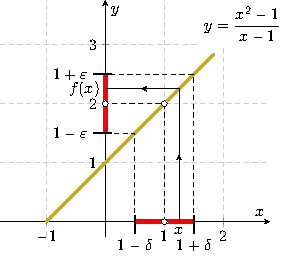
\includegraphics[width=0.45\linewidth]{mai_fig017.pdf}
   \captionof{figure}{K příkladu \ref{MAI:exam028}
   \cite[s.~118]{Brabec1989}
   \label{mai:fig017}}
  \par}
  
  Zvolíme-li libovolně malé okolí bodu \(2\), pak vždy lze najít okolí bodu \(1\) takové, že pro 
  každé \(x \neq 1\) z tohoto okolí bude ležet hodnota \(f(x)\) ve zvoleném okolí čísla \(2\). 
  Ještě jinak formulováno: K libovolně malému \(\varepsilon > 0\) existuje \(\delta > 0\) tak, 
  že pro každé \(x\), pro něž \(0 < \abs{x — 1} \ll \delta\), platí \(\abs{f(x) — 2} < 
  \varepsilon\) (viz obr. \ref{mai:fig017}). O funkci \(f\) s touto vlastností říkáme, že má v bodě 
  \(1\) limitu \(2\) a píšeme symbolicky \(lim_{x \to 1}f(x) = 2\) nebo \(f(x) \rightarrow 2\) pro 
  \(x \rightarrow 1\).
\end{example}
















    %-------------------------------------

    Definičním oborem funkce z příkladu \ref{MAI:exam028} je tedy množina \(\mathcal{D} = \realset 
    — {1}\) (pro \(a = 1\) by ve jmenovateli zlomku byla nula). Grafem funkce je tedy přímka s 
    „vynechaným“ bodem \([1, 2]\) (obr. \ref{mai:fig017}). V bodě \(a = 1\) funkční hodnota není 
    definována. Pokud bychom chtěli rozšířit definiční obor funkce na celou reálnou osu, musíme 
    předepsat, jaké hodnoty má funkce nabývat v bodě \(a = 1\). Původní vzorec, jímž je funkce 
    zadána, výpočet hodnoty \(f(1)\) neumožňuje. Dodatečné zadání funkční hodnoty, její 
    \emph{dodefinování}, můžeme provést zcela libovolně. Zvolme například \(f(1) = 2\). Jiná 
    možnost, jak funkci dodefinovat, je například \(f(1) =-1\). Které číslo je ovšem limitou funkce 
    \(f(x)\) v bodě \(a = 1\)? Je to číslo \(2\), které je v případe \(f(x) = x+1\) její funkční 
    hodnotou? Nebo číslo \(-1\)? A nebo nějaká jiná hodnota? Intuice nám napovídá, že je to číslo 
    \(2\). Když dvojku použijeme pro dodefinování funkce, přetržený graf se „zacelí“. Vidíme, že 
    vezmeme-li dostatečně malý interval proměnné \(x\) v blízkosti bodu \(a=1\) můžeme docílit 
    toho, že všechny odpovídající funkční hodnoty \(f(x)\) budou ležet tak blízko hodnotě \(2\), 
    jak si předem určíme. Skutečně, zkusme docílit toho, aby hodnoty \(f(x)\) ležely v intervalu 
    \((\num{1.99}, \num{2.01})\), tj.
    \begin{equation*}
      \num{1.99} < x + 1 < \num{2.01} \Rightarrow \num{0.99} < x < \num{1.01},\qquad x\neq1.
    \end{equation*}
    Podařilo se. A kdybychom interval \(I(\varepsilon) = (2 - \varepsilon, 2 + \varepsilon)\) 
    funkčních hodnot kolem \(2\) ještě zmenšili, podařilo by se opět najít (o něco menší) interval 
    kolem bodu \(a = 1\) tak, aby pro všechny hodnoty \(x\) v něm (samozřejmě s případnou výjimkou 
    hodnoty \(a =2\)) platilo \(f(x)\in I(\varepsilon)\). A takto bychom mohli \(\varepsilon\) 
    stále zmenšovat. Jak by takový postup dopadl s hodnotou \(-1\), která, jak intuitivně cítíme, 
    limitou funkce v bodě \(a = 1\) není, protože je graf funkce od bodu \([-1,0]\) dost vzdálen? 
    Vezměme třeba interval (\num{-0.5}, \num{0.5}) a hledejme hodnoty \(x\) obdobně jako v 
    předchozím případě. Požadujeme
    \begin{equation*}
      \num{-0.5} < x + 1 < \num{0.5} \Rightarrow \num{-1.5} < x < \num{-0.5}.
    \end{equation*}
    Tento interval vůbec neobsahuje bod \(a = 1\). Dostali jsme se mimo blízkost bodu \(a = 1\).

    %-------------------------------------
      % !TeX spellcheck = cs_CZ
\begin{mathexam}{Najdi limitu funkce \(\varphi(x) = \sqrt[3]{x}\) v bodě \(a = 0\) pomocí
  \eqref{mai:eq037}}{exam029} 
   
  Nechť \(\varphi(x) = \sqrt[3]{x}\), \(a = 0\). Pak \[f(x) = \dfrac{\sqrt[3]{x}}{x}\]. Pro \(x \neq
  0\) je \[f(x) = \frac{1}{\sqrt[3]{x^2}}\]. Jestliže \(x \to 0\), pak hodnoty \(f(x)\) neomezeně
  vzrůstají, protože jmenovatel zlomku se blíží kladnými hodnotami k nule a čitatel je stále roven
  \(1\) (viz obr. \ref{mai:fig018}). Místo rčení \emph{„funkce neomezeně roste“} pro \(x \to 0\)
  říkáme též ]\emph{„funkce se blíží k \(+\infty\)“} pro \(x \to 0\) a píšeme 
  \begin{equation*}
    \lim\limits_{x\to 0} f(x) = +\infty \text{ nebo } f(x)\to +\infty\text{ pro } x\to0.
  \end{equation*}
  Říkáme, že limita funkce \(f\) v bodě \(0\) je rovna \(+\infty\). 
    
  {\centering
  \captionsetup{type=figure}
%   \documentclass[11pt]{standalone}
\usepackage{xltxtra}
\usepackage[usenames,x11names]{xcolor}
\usepackage{tikz}
  \usetikzlibrary{intersections}
  \usetikzlibrary{decorations.markings}
\usepackage{pgfplots}
  \pgfplotsset{compat=newest}
  
\usepackage{amsmath}

\begin{document}
  \begin{tikzpicture}[thick,scale=0.7, 
      every node/.style={transform shape},
      ]
  
  \tikzset{->-/.style={decoration={
    markings,
    mark=at position #1 with {\arrow{stealth}}},postaction={decorate}}}
    
    \begin{axis}[
      xmin = -2.5, xmax = 2.5, ymin = 0, ymax = 3.5,  % osy
      domain = -1:3.5,
      restrict y to domain=0:3.4,
      axis equal image,
      grid = major,   % both
      grid style={line width=.1pt, draw=gray!20},
      major grid style={dashed, line width=.2pt, draw=gray!40},
      clip = true,
      clip mode=individual,
      xtick={-2,-1,1,2,3,4}, % make steps of length 0.2
      ytick={0,1,2,3,4,5}, 
      axis x line = middle,
      axis y line = middle,
      xlabel={\(x\)}, ylabel={\(y\)},
      enlarge y limits={rel=0.07},
      enlarge x limits={rel=0.07},
      ]
  
        \addplot[color=Gold3, samples=100, smooth, ultra thick, unbounded coords=jump,
                 no markers, domain = 0.1:2, name path global=func1] 
           gnuplot{1/((x^2.0)^(1/3.0))};
  
        \addplot[color=Gold3, samples=100, smooth, ultra thick, unbounded coords=jump,
                 no markers, domain = -2:-0.1, name path global=func2] 
           gnuplot{real(1/((x^2.0)^(1/3.0)))};
  
        \node [fill=white] at (rel axis cs: 0.75,0.5) {\(y=\dfrac{1}{\sqrt[3]{x^2}}\)};
  
        \path[name path=line] (-1,1.5) -- (1,1.5); 
            % Intersections points
            \path [name intersections={of=func1 and line,by={P1}}] (P1) node [] {};
  
        \path[name path=line] (-1,1.5) -- (1,1.5); 
            % Intersections points
            \path [name intersections={of=func2 and line,by={Q1}}] (Q1) node [] {};
        
        \draw[black,fill=black] (P1) circle (.3ex);
        \draw[black,fill=black] (Q1) circle (.3ex);
        \path (P1 |- 3,0) -- (P1) -- (P1 -| 0,3) node (X) {};
  
        \draw[thick,red, fill=white] ([shift=(0:1mm)]X) arc (0:180:1mm);
        \draw[->-=.5, dashed]  (P1 |- 3,-0.1)  
          node[below] {\(\delta\)} -- (P1) -- (P1 -| 0,3);
        \draw[->-=.5, dashed]  (Q1 |- -3,-0.1) 
          node[below] {\(\delta\)} -- (Q1) -- (Q1 -| 0,3);
  
        \draw[line width = 2pt, red, line cap=butt] (Q1 |- 3,0) -- (P1 |- 3,0);
        
        \path[name path=line] (-0.7,2.5) -- (0.7,2.5); 
            % Intersections points
            \path [name intersections={of=func1 and line,by={P1}}] (P1) node [] {};
            \draw[->-=.4, dashed, thin,gray] (P1 |- 3,-0.05) node[below] {\(x\)} -- (P1);
            \draw[->-=1, thin, gray] (P1) -- (P1 -| 0,3) node[left, fill=white] {\(f(x)\)};
        \draw[thick,red] (X) node[below left] {\(q\)} -- ++(0cm,2.5cm);
  
       \draw[black,fill=white] (0,0) node[below left] {\(O\)} circle (.4ex);
    \end{axis}
  \end{tikzpicture}
\end{document}
  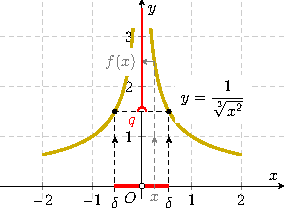
\includegraphics[width=0.8\linewidth]{mai_fig018.pdf}
  \captionof{figure}{K příkladu \ref{MAI:exam029}
  \cite[s.~118]{Brabec1989}
  \label{mai:fig018}}
  \par}
  
  Přesně to znamená toto: Zvolíme-li libovolně velké \(q > 0\), můžeme nalézt \(\delta > 0\) tak, že
  pro každé \(x \neq 0\), pro něž \(\abs{x} < \delta\), platí \(f(x) > q\). 
  
  To lze říci i takto: Zvolíme-li libovolně okolí bodu \(+\infty\), existuje okolí bodu \(0\) tak,
  že pro každé \(x \neq 0\) z tohoto okolí je \(f(x)\) ve zvoleném okolí \(+\infty\) (viz obr.
  \ref{mai:fig018}).
\end{mathexam}
















    %-------------------------------------

    Je třeba říci, že při zkoumání limit funkcí nás nezajímají jen funkce „tvaru“ 
    (\ref{mai:eq037}), i když tento případ je v diferenciálním počtu velmi častý, jak poznáme v 
    kap. \ref{mai:IchapIV}. Někdy nás zajímá i chování funkcí v okolí nevlastních bodů \(-\infty\), 
    \(+\infty\) 

    %-------------------------------------
      % !TeX spellcheck = cs_CZ
\begin{mdframed}[style=mdexam]
  \begin{example}\label{MAI:exam030}
    Je dána funkce \(f: f(x) = \frac{x + 1}{x}\). Sledujme její chování, když hodnoty argumentu
    \(x\) budou vzrůstat nade všechny meze neboli, jak říkáme, \(x\) se bude blížit k \(+\infty\)
    (což zapisujeme \(x \to + \infty\) (viz obr. \ref{mai:fig019}). Můžeme psát \(f(x) = 1 + 1/x\).
    Vzrůstají-li neomezeně hodnoty proměnné \(x\), blíží se hodnoty výrazu \(1/x\) čím dál tím více
    nule, takže funkční hodnoty \(f(x)\) jsou čím dál tím blíže číslu \(1\). V tomto případě píšeme
    \(lim_{x\to+\infty} f(x) = 1\) nebo \(f(x) \to 1\) pro \(x\to +\infty\) a říkáme, že funkce
    \(f\) má v bodě \(+\infty\) limitu rovnou \(1\). Přesně to znamená toto: Zvolíme-li libovolně
    malé \(\varepsilon > 0\), můžeme nalézt \(p > 0\) tak, že pro \(x > p\) platí \(\abs{f(x) - l} <
    \varepsilon\). (Viz obr. \ref{mai:fig019}.) Můžeme to říci i takto: Zvolíme-li libovolně okolí
    bodu \(1\), existuje okolí bodu \(+\infty\) tak, že pro každé \(x\) (konečné) z tohoto okolí je
    \(f(x)\) ve zvoleném okolí bodu \(1\).
    
    {\centering
    \captionsetup{type=figure}
  %   % !TeX spellcheck = cs_CZ

\documentclass[11pt]{standalone}
\usepackage{xltxtra}
\usepackage[usenames,x11names]{xcolor}
\usepackage{tikz}
  \usetikzlibrary{intersections}
  \usetikzlibrary{decorations.markings}
\usepackage{pgfplots}
  \pgfplotsset{compat=newest}
  
\usepackage{amsmath}

\begin{document}
  \begin{tikzpicture}[thick,scale=0.7, 
      every node/.style={transform shape},
      ]
  
  \tikzset{->-/.style={decoration={
    markings,
    mark=at position #1 with {\arrow{stealth}}},postaction={decorate}}}
    
    \begin{axis}[
      xmin = -0.5, xmax = 5.5, ymin = 0, ymax = 4.5,  % osy
      domain =0.2:5,
      restrict y to domain=0:4,
      axis equal image,
      grid = major,   % both
      grid style={line width=.1pt, draw=gray!20},
      major grid style={dashed, line width=.2pt, draw=gray!40},
      clip = true,
      clip mode=individual,
      xtick={1,2,3,4,5}, % make steps of length 0.2
      ytick={0,1,2,3,4}, 
      axis x line = middle,
      axis y line = middle,
      xlabel={$x$}, ylabel={$y$},
      enlarge y limits={rel=0.07},
      enlarge x limits={rel=0.07},
      ]
  
      \addplot[color=Gold3, samples=100, smooth, ultra thick, unbounded coords=jump,
               no markers, domain = 0.1:5, name path global=func1] 
         gnuplot{1+1/x};
  
      \node [fill=white] at (rel axis cs: 0.4,0.75) {\(y=\dfrac{x+1}{x}\)};
  
      \path[name path=line] (0,1.7) -- (3,1.7); 
          % Intersections points
          \path [name intersections={of=func1 and line,by={P1}}] (P1) node [] {};
      
      \draw[black,fill=black] (P1) circle (.3ex);      
      \path (P1 |- 3,-0.1) node [below, fill=white] (X) {p} -- (P1) -- (P1 -| 0,3);
  
      \draw[thick,red, fill=white] ([shift=(90:2.5mm)]X) 
           arc (270:360:1mm) node(Y) {} arc (360:450:1mm);
      \draw[thin] (P1 |- 3,-0.1) -- (P1) -- (P1 -| 0,3);
      \draw[line width = 2pt,red] (Y |- 3,0)  -- ++(3.5,0);
      
   
      \draw[line width = 1pt, black, dashed] (0,1) -- ++(5,0);
      \draw[line width = 3pt, red, line cap=butt] (0,0.3) -- (0,1.7);
      \draw [thick] (-.2, 0.3) node[left] {\(1-\varepsilon\)} -- (0.1, 0.3);
      \draw [thick] (-.2, 1.7) node[left] {\(1+\varepsilon\)} -- (0.1, 1.7 );
  
      \draw[black,fill=white] (0,1) circle (.4ex);

      \path[name path=line] (2.4,0) -- ++(0,2.5); 
          % Intersections points
          \path [name intersections={of=func1 and line,by={P1}}] (P1) node [] {};
          \draw[->-=.4, dashed, gray] (P1 |- 3,-0.05) node[below] {\(x\)} -- (P1);
          \draw[->-=1,  dashed, gray] (P1) -- (P1 -| 0,3) 
            node[left] {\small\(f(x)\)};
            
    \end{axis}
  \end{tikzpicture}
\end{document}
    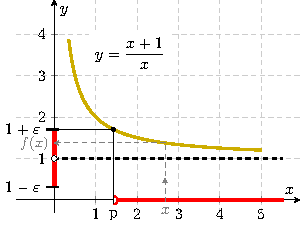
\includegraphics[width=0.45\linewidth]{mai_fig019.pdf}
    \captionof{figure}{K příkladu \ref{MAI:exam030}
    \cite[s.~119]{Brabec1989}
    \label{mai:fig019}}
    \par}
  \end{example}
\end{mdframed}
















    %-------------------------------------
    
    %-------------------------------------
      % !TeX spellcheck = cs_CZ
\begin{mdframed}[style=mdexam]
  \begin{example}\label{MAI:exam031}
    Je dána funkce \(f: f(x) = \frac{x + 1}{x}\). Sledujme její chování, když hodnoty argumentu
    \(x\) budou vzrůstat nade všechny meze neboli, jak říkáme, \(x\) se bude blížit k \(+\infty\)
    (což zapisujeme \(x \to + \infty\) (viz obr. \ref{mai:fig019}). Můžeme psát \(f(x) = 1 + 1/x\).
    Vzrůstají-li neomezeně hodnoty proměnné \(x\), blíží se hodnoty výrazu \(1/x\) čím dál tím více
    nule, takže funkční hodnoty \(f(x)\) jsou čím dál tím blíže číslu \(1\). V tomto případě píšeme
    \(lim_{x\to+\infty}f(x) = 1\) nebo \(f(x) \to 1\) pro \(x\to +\infty\) a říkáme, že funkce \(f\)
    má v bodě \(+\infty\) limitu rovnou \(1\). Přesně to znamená toto: Zvolíme-li libovolně malé
    \(\varepsilon > 0\), můžeme nalézt \(p > 0\) tak, že pro \(x > p\) platí \(\abs{f(x) - l} <
    \varepsilon\). (Viz obr. \ref{mai:fig019}.) Můžeme to říci i takto: Zvolíme-li libovolně okolí
    bodu \(1\), existuje okolí bodu \(+\infty\) tak, že pro každé \(x\) (konečné) z tohoto okolí je
    \(f(x)\) ve zvoleném okolí bodu \(1\).
    
    {\centering
    \captionsetup{type=figure}
  %   % !TeX spellcheck = cs_CZ
% xelatex -enable-write18 -shell-escape mai_fig020.tex
\documentclass[11pt]{standalone}
\usepackage{xltxtra}
\usepackage[usenames,x11names]{xcolor}
\usepackage{tikz}
  \usetikzlibrary{intersections}
  \usetikzlibrary{decorations.markings}
\usepackage{pgfplots}
  \pgfplotsset{compat=newest}
  
\usepackage{amsmath}

\begin{document}
  \begin{tikzpicture}[thick,scale=0.7, 
      every node/.style={transform shape},
      ]
  
  \tikzset{->-/.style={decoration={
    markings,
    mark=at position #1 with {\arrow{stealth}}},postaction={decorate}}}
    
    \begin{axis}[
      xmin = -2, xmax = 3.5, ymin = -2, ymax = 6,  % osy
      domain =-2:8,
      restrict y to domain=-1.5:6,
      axis equal image,
      grid = major,   % both
      grid style={line width=.1pt, draw=gray!20},
      major grid style={dashed, line width=.2pt, draw=gray!40},
      clip = true,
      clip mode=individual,
      xtick={-1,0,1,2,3,4}, % make steps of length 0.2
      ytick={-1,0,1,2,3,4,5,6,7,8}, 
      axis x line = middle,
      axis y line = middle,
      xlabel={$x$}, ylabel={$y$},
      enlarge y limits={rel=0.07},
      enlarge x limits={rel=0.07},
      ]
  
      \addplot[color=Gold3, samples=100, smooth, ultra thick, unbounded coords=jump,
               no markers, domain = -2:2, name path global=func1] 
         gnuplot{x^3};
  
      \node [fill=white] at (rel axis cs: 0.85,0.9) {\(y=x^3\)};
  
      \path[name path=line] (1.5,0) -- (1.5,6); 
          % Intersections points
          \path [name intersections={of=func1 and line,by={P1}}] (P1) node [] {};
          \draw[->-=.4, dashed, gray] (P1 |- 3,-0.05) node[below, fill=white] {\(x\)} -- (P1);
          \draw[->-=1,  dashed, gray] (P1) -- (P1 -| 0,3) 
            node[left=0.5cm, fill=white] {\small\(f(x)\)};
          \draw[dashed, gray] (P1 -| 0,3) + (-0.6cm,0cm) -- (P1 -| 0,3);
      \path[name path=line1] (0,1) -- (2,1); 
          % Intersections points
          \path [name intersections={of=func1 and line1, by={P1}}] (P1) node [] {};    
          \path (P1 |- 3,-0.1) node [below, fill=white] (X) {p} -- (P1) -- (P1 -| 0,3) 
              node[left, fill=white] (Y) {\(q\)};
  
      \draw[thick,red, fill=white] ([shift=(90:2mm)]X) 
           arc (270:360:1mm) node(x1) {} arc (360:450:1mm);
      \draw[dashed] (P1 |- 3,-0.1) -- (P1) -- (P1 -| 0,3);
      \draw[line width = 1pt,red] (x1 |- 3,0)  -- (3,0);
      
      \draw[thick,red] (0,1) -- (0,6);
      \draw[thick,red, fill=white] ([shift=(0:3.3mm)]Y) arc (0:180:1mm);;
    \end{axis}
  \end{tikzpicture}
\end{document}
    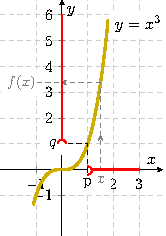
\includegraphics[width=0.35\linewidth]{mai_fig020.pdf}
    \captionof{figure}{K příkladu \ref{MAI:exam031}
    \cite[s.~119]{Brabec1989}
    \label{mai:fig020}}
    \par}
  \end{example}
\end{mdframed}
    %-------------------------------------
    
    V uvedených případech bychom mohli zkoumat i limity funkcí pro \(x \to - \infty\).  Všimněme si 
    ještě, že ve všech případech nebylo nutné, aby funkce \(f\) byla definována v bodě, ke kterému 
    se blíží hodnoty argumentu, ale bylo zapotřebí, aby funkce \(f\) byla definována v bodech 
    libovolně blízkých tomuto bodu. Tomuto požadavku bude vyhověno, jestliže daný bod, v němž 
    zkoumáme limitu, bude \emph{hromadným bodem definičního oboru}. Není ovšem nutné, aby funkce 
    byla definována v celém nějakém \emph{prstencovém okolí uvažovaného bodu}.
    
    Nechť \(a\) je bod, blízko kterého se pohybuje hodnota proměnné \(x\). Pro definici limity je 
    důležitý pojem \textbf{okolí bodu} \(a\) (obr. 2.16). Zvolme kladná čísla \(\delta_1\) a 
    \(\delta_2\). Nazýváme
    
    
      
  %================ Podkapitola: Spojitost funkce ==================================================
  \section{Spojitost funkce}
  
%} % tikzset
%~~~~~~~~~~~~~~~~~~~~~~~~~~~~~~~~~~~~~~~~~~~~~~~~~~~~~~~~~~~~~~~~~~~~~~~~~~~~~~~~~~~~~~~~~~~~~~~~~~
\printbibliography[title={Seznam literatury}, heading=subbibliography]
\addcontentsline{toc}{section}{Seznam literatury}          	
%  % !TeX spellcheck = cs_CZ
%{\tikzset{external/prefix={tikz/MAI/}}
% \tikzset{external/figure name/.add={ch10_}{}}
%---------------------------------------------------------------------------------------------------
% file ppst.tex
%---------------------------------------------------------------------------------------------------
\chapter{Počet Pravděpodobnosti}
\minitoc
  Slovo pravděpodobnost používáme velmi často. Jaký však je jeho přesný význam? Jsme přesvědčeni, 
  že pravděpodobnost výhry ve sportce je velmi malá. Ani pravděpodobnost, že se vyplní předpověď 
  počasí, nepovažujeme mnohdy za výraznou. Přesto je mezi oběma příklady obrovský kvantitativní 
  rozdíl. Zkusme význam pojmu pravděpodobnost ukázat pomocí konkrétních číselných příkladů.
  
  \begin{itemize}
    \item \textbf{Příklad se střelcem}: Sportovní střelec střílí na terč série \num{100} ran. 
          Předpokládejme, že podmínky při střelbě jsou stále stejné. Stejná je zbraň, terč, 
          vzdálenost, povětrnostní podmínky i momentální zdravotní stav střelce. Při hodnocení 
          střelcova „mistrovství“ někdo řekne, že střelec zasáhne terč s pravděpodobností 
          \num{92}\%. Jak tomu rozumět? Znamená to, že v souboru sérií výstřelů jsou velmi časté 
          ty, v nichž zasáhl střelec terč \num{92}-krát. Samozřejmě, není řídké, že se objeví i 
          série s \num{93} nebo \num{94} zásahy, ale také s \num{91} nebo \num{90}. Vyloučen není 
          ani případ s úspěšností \num{96} či \num{88}, a dokonce i stovku bychom mohli zaznamenat. 
          Situace výrazně odlišné od \num{92} zásahů však budou řídké, a to tím více, čím více se 
          úspěšnost série liší od \num{92} oběma směry.
    \item \textbf{Příklad se zmetky}: Koupíte si výrobek u firmy, o které je známo, že vyrábí 
          zmetky s pravděpodobností 0,16\%? Situaci lze posuzovat obdobně jako úspěšnost střelce. 
          Budeme-li například zkoumat série obsahující 1000 výrobků, bude každá z nich obsahovat „v 
          průměru“ 16\% zmetků. Z příkladu se střelcem již zhruba víme, jak posuzovat slovo v 
          průměru.
  \end{itemize}
  
  V této kapitole se budeme pravděpodobnostmi zabývat podrobněji. Zjistíme, že i když se týkají 
  náhodných jevů, platí i pro ně jisté zákonitosti.
    
  \section{Pravděpodobnost}
    V úvodních příkladech jsme si vyložili, jak intuitivně chápat pojem pravděpodobnost. Jednalo se 
    v nich o posouzení průměrné úspěšnosti ve velkém souboru operací či úkonů prováděných za 
    stejných podmínek, šlo tedy o jakousi „průměrnou“ pravděpodobnost. Nyní definujeme 
    pravděpodobnost matematicky.
    
    \subsection{Co se pravdě podobá — definice pravděpodobnosti}
      Pro definici pravděpodobnosti použijeme pojmu \emph{náhodný pokus}, jehož význam si ukážeme 
      na příkladu. Dobrým příkladem náhodných pokusů je třeba házení mincí, hraní kostkou, výběr 
      karet z balíčku, vidíme-li pouze jejich rub, apod. Budeme třeba házet kostkou. Abychom si 
      situaci zbytečně nekomplikovali, budeme předpokládat, že všechny výsledky hodu kostkou 
      (náhodné pokusy) jsou stejně časté, žádný z nich není nijak preferován\footnote{Kostka by 
      tedy měla být homogenní, plocha, na kterou po hodu dopadne, vodorovná, kvalita povrchu všech 
      stěn kostky stejná (žádná stěna by třeba neměla být natřena lepidlem), apod.}. Počet možných 
      výsledků jednotlivého hodu je \(N = 6\) (kostka má \num{6} stěn, na každé je vyznačen odlišný 
      počet ok, tedy \num{1} až \num{6}). Jednotlivé situace, které mohou nastat, nazýváme 
      náhodnými jevy. Náhodným jevem \(A\) tak může být situace \emph{„padne číslo \num{2}“}, jiným 
      náhodným jevem \(B\) situace \emph{„padne číslo dělitelné třemi“}, apod. Počet situací, kdy 
      výsledek hodu lze hodnotit tak, že určitý jev nastal, označíme \(M\). Například pro jev \(A\) 
      \emph{„padne číslo \num{2}“} je \(M(A)= 1\), pro jev \(B\) \emph{„padne číslo dělitelné 
      třemi“} je \(M(B) = 2\) (počet ok \num{3} nebo \num{6}). Můžeme také definovat jev \(O\) 
      \emph{„nepadne žádné číslo“} (\(M(0) = 0\)) nebo jev \(J\) \emph{„padne jakékoli číslo“} 
      (\(M(J) = 6\)).
      
      \begin{definition}
        Pravděpodobností jevu rozumíme podíl
        \begin{equation}\label{mai:eq011}
          p = \frac{M}{N} = \frac{\text{počet případů příznivých}}{\text{počet případů možných}}.
        \end{equation}  
        Počtem případů možných jsme zkráceně nazvali počet všech možných výsledků náhodného 
        pokusu, počtem případů příznivých pak počet všech takových výsledků pokusu, při nichž daný 
        jev nastal.
      \end{definition}
      Je zřejmé, že hodnota pravděpodobnosti jakéhokoli jevu je nezáporná a může nabývat hodnoty 
      nejvýše \num{1}, tj. \(0 <p< 1\). Jev s \emph{nulovou pravděpodobností} se nazývá 
      \textbf{nemožný}, jev s \emph{jednotkovou pravděpodobností} je \textbf{jistý}. V našem 
      příkladu s kostkou tak dostáváme
      \begin{equation*}
        p(A) = \frac{1}{6}, \qquad p(B) = \frac{2}{6} = \frac{1}{3}, \qquad
        p(O) = 0, \qquad p(J) = 1.
      \end{equation*}  

      %---------------------------------------------------------------
      % !TeX spellcheck = cs_CZ
\begin{example}
 \label{mai:exam006}
  \textbf{Barevné ponožky}:\newline\small
  V zásuvce jsou ponožky tří barev. Červené (\textbf{Č}), zelené (\textbf{Z}) a modré (\textbf{M}). 
  Je jich tam od každé barvy hodně. Student jde na schůzku a chce si vzít čisté ponožky. Náhle 
  zhasne světlo. Student vytáhne potmě dvě ponožky. Jaká je pravděpodobnost, že ponožky budou mít 
  stejnou barvu? Vyjmenujme případy, které mohou při vytažení dvou ponožek nastat: (\textbf{Č+Č}), 
  (\textbf{Č+Z}), (\textbf{Z+Č}), (\textbf{Č+M}), (\textbf{M+Č}), (\textbf{Z+Z}), (\textbf{Z+M}), 
  (\textbf{M+Z}), (\textbf{M+M}). Je tedy \(n = 9\). Příznivé situace jsou tří, (\textbf{Č+Č}), 
  (\textbf{Z+Z}), (\textbf{M+M}). Pravděpodobnost je tedy 1/3. (Převzato z 
  \cite[s.~200]{Musilova2009MA1}) 
\normalsize
\end{example}
      %---------------------------------------------------------------
    \subsection{Cifry, kostky, karty - kombinatorické opakování}
      Příklad s ponožkami byl velmi jednoduchý. Podařilo se nám vyjmenovat všechny případy možné i 
      všechny případy příznivé, neboť obojího bylo docela málo. Daleko běžnější jsou však situace, 
      kdy výčet případů není schůdný. A tehdy potřebujeme \textbf{kombinatoriku}.
      
      Nechť \(\mathcal{M}\) je \(n\)-prvková množina, z níž budeme provádět výběry \(k\) prvků 
      podle určitých pravidel. Prvky množiny \(\mathcal{M}\) nemusíme nijak konkretizovat. Abychom 
      si však o výběrech a pravidlech pro jejich tvorbu dokázali udělat nějakou názornou představu, 
      je taková konkretizace vhodná. Prvky množiny \(\mathcal{M}\): mohou být třeba žáci ve třídě, 
      barvy, hrací karty, apod. Výběry mohou představovat třeba družstva pro odbíjenou, signály 
      tvořené barevnými praporky, možnosti rozdání karet při mariáši, apod. Jednotlivé typy výběrů 
      získaly své názvy právě na základě pravidel stanovených pro jejich vytváření. Rozhodující 
      jsou dvě základní kritéria:
      \begin{itemize}\addtolength{\itemsep}{-0.5\baselineskip}
        \item Je pro tvorbu výběru podstatné pořadí prvků ve výběru či nikoliv?
        \item Mohou se prvky ve výběru opakovat či nikoliv?
      \end{itemize}
      
      Typy výběrů shrnuje následující diagram:
      \begin{figure}[ht!] %\ref{mai_fig021}
        \centering
        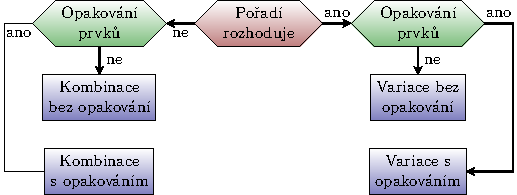
\includegraphics[width=0.7\linewidth]{mai_fig021.pdf}
        \caption{Typy výběrů. \cite[s.~201]{Musilova2009MA1}}
        \label{mai_fig021}
      \end{figure}

      Představuje-li daný výběr například volejbalové družstvo osmi děvčat (šest hráček a dvě 
      náhradnice), které bude reprezentovat v soutěži třídu osmou bé, do níž chodí \num{25} děvčat 
      a \num{18} chlapců, jedná se o výběr \(k — 8\) prvků z počtu \(n = 25\) prvků. Chlapce nelze 
      postavit do družstva volejbalistek. Každý výběr možného družstva bude představovat 
      \emph{kombinaci bez opakování}, neboť pořadí hráček nehraje roli a třeba Aničku Novákovou 
      máme ve třídě jen jednu. Budeme-li však chtít vytvářet z deseti cifer \(0, 1, \ldots, 9\) 
      trojciferná čísla, pak tyto výběry tří prvků z deseti (\(k = 3\), \(n = 10\)) jsou 
      \emph{variacemi s opakováním}. Čísla \num{125}, \num{512}, \num{251}, \num{215}, \num{521} a 
      \num{152} jsou totiž různá, a například \num{222} je také trojciferné číslo. Kombinace s 
      opakováním bychom mohli vytvářet třeba i při výběru různobarevných ponožek ze zásuvky a 
      konečně \emph{variacemi bez opakování} by mohly být dejme tomu trojbarevné signály (\(k = 
      3\)) tvořené trojicemi barevných hadříků vybíraných z \(n\) barev (pro \(n = 3\) třeba zrovna 
      z těch ponožek). Nyní bychom však rádi věděli, jak pro zadané hodnoty \(n\) a \(k\) určit 
      počet všech možných výběrů předepsaného typu. Ukážeme si to na příkladech.

      %---------------------------------------------------------------
      % !TeX spellcheck = cs_CZ
\begin{mdframed}[style=mdexam]
  \begin{example}\label{mai:exam007}
    \textbf{Šance milion}:\newline
    „Znáte nějakou jinou hru, kde můžete denně vyhrát milion?“ Tento nebo jiný, obdobně nepříliš
    vtipný reklamní slogan propaguje v televizi hru, jejímž cílem je uhodnout šestici tažených cifer
    ve správném pořadí. (Hru raději nehrajte, pravděpodobnost výhry je mizivá.) Tah se provádí
    následovně: V každém ze šesti bubnů, očíslovaných pořadovými čísly \num{1} až \num{6}, je
    připraveno deset míčků opatřených ciframi \(0, 1, \ldots, 9\). Z prvního bubnu se náhodně
    vylosuje jedna cifra (deset možností). Poté se náhodně vylosuje jedna cifra z druhého bubnu
    (opět deset možností). Možností vzniku uspořádané dvojice cifer (jedna cifra z prvního a druhá z
    druhého bubnu) je již sto (každou možnost výsledku u prvního bubnu lze kombinovat s každou
    možností výsledku z druhého bubnu). Losování pokračuje u třetího, čtvrtého, pátého a šestého
    bubnu. Celkový počet možností je \num{1e6}, tedy \textbf{milion}. (Šance získat výhru, tedy
    vyhrát milion, je ovšem pouze jedna milióntina, neboť z milionu možností je pouze jedna skutečně
    tažena.) 
  \end{example}
\end{mdframed}
      %---------------------------------------------------------------
      
      Zobecněním předchozího příkladu získáváme vzorec pro počet \textbf{variací s opakováním} 
      \emph{k}-té třídy z \(n\) prvků. Při tahu totiž záleží na pořadí bubnů a každý buben obsahuje 
      všechny cifry. Výsledky tahů z jednotlivých bubnů se tedy mohou opakovat. Pokud by bubnů bylo 
      \(k\) a v každém \(n\) různých cifer, dostali bychom pro \textbf{variace s opakováním 
      \(k\)-té třídy z \(n\) prvků} celkový počet
      \begin{equation}\label{mai:eq007}
        \boxed{V_k' = n^k}\, .
      \end{equation}

      %---------------------------------------------------------------
      % !TeX spellcheck = cs_CZ
\begin{example}\label{mai:exam008}
  \textbf{Modifikovaná šance milion}:\newline
  Představme si hru z předchozího příkladu upravenou takto: K dispozici bude jen jeden buben s 
  ciframi \(0, 1, \ldots, 9\), každá cifra je v bubnu obsažena pouze jednou. Opět máme losovat 
  uspořádanou \textbf{šestici cifer}. Nyní se však jedná o \textbf{variace šesté třídy z deseti 
  prvků bez opakování}. S jediným bubnem musíme totiž provést šest losování, přičemž při každém 
  losování ubude z bubnu jedna cifra. Při prvním tahu je deset možností, při druhém již jen devět, 
  atd., při šestém již pouze pět možností. Celkem je tedy \(10 \cdot 9 \cdots 5 = \num{151200}\) 
  možností.
\end{example}
      %---------------------------------------------------------------
      
      Uvážíme-li, že v předchozím příkladu je \(n = 10\) a \(k = 6\), dostáváme pro \textbf{počet 
      variací bez opakování \(k\)-té třídy z \(n\) prvků} obecný vztah
      \begin{align}
        V_k(n) &= n(n-1)(n-2)\cdots(n-k+1)  \nonumber \\
        \shortintertext{neboli}
        V_k(n) &= \frac{n!}{(n-k)!}\, .    \label{mai:eq008}
      \end{align}
      Poznamenejme, že \(n!\) značí \textbf{faktoriál}, \(n! = n(n — 1)\cdots 3 \cdot 2 \cdot 1\). 
      Pro nulu definujeme \(0! = 1\). Je zřejmé, že při vytváření variací bez opakování musí být 
      \(k\leqq n\). Variace bez opakování \(n\)-té třídy z \(n\) prvků se nazývají 
      \textbf{permutace}. Každá z nich představuje určité uspořádání těchto \(n\) prvků. Platí
      \begin{equation}\label{mai:eq009}
        \boxed{P(n) = V_n(n) = n!}\, .
      \end{equation}
      
      Nyní odvodíme vzorec pro počet \textbf{kombinací \(k\)-té třídy z \(n\) prvků bez opakování}. 
      Již jsme si řekli, že \emph{kombinací} rozumíme takový výběr z celkového počtu \(n\) prvků, 
      který obsahuje určitých \(k\) prvků nezávisle na jejich pořadí. Představme si, že máme k 
      dispozici všechny variace bez opakování \(k\)-té třídy ze zmíněných \(n\) prvků. Vezměme 
      kteroukoli z nich. Soubor všech variací \(k\)-té třídy z \(n\) prvků však obsahuje i další 
      variace, lišící se od té naší jen pořadím prvků. Celkem je takových variací (i s tou první) 
      \(k!\) a z hlediska kombinací představují totéž. Soubor variací se tak rozpadá na podsoubory, 
      z nichž každý obsahuje \(k!\) variací lišících se navzájem pouze pořadím prvků. Každý z 
      těchto podsouborů představuje však jedinou kombinaci. Počet kombinací \(k\)-té třídy z \(n\) 
      prvků bez opakování je tedy
      \begin{equation}\label{mai:eq010}
        \boxed{C(k) = \frac{V_k(n)}{P(k)} = \frac{n!}{(n-k)!\,k!} = 
               \begin{pmatrix}
                n \\
                k
               \end{pmatrix}}\, .
      \end{equation}
      
      Pro odvození vzorce pro \textbf{kombinace s opakováním} použijeme opět příkladu.
      %---------------------------------------------------------------
      % !TeX spellcheck = cs_CZ
\begin{mathexam}{Kuličky v přihrádkách}{exam009}
  Máme kuličky \(n\) různých barev, v každé barvě máme tolik kuliček, kolik bude potřeba. Naším
  úkolem je vytvářet výběry \(k\) kuliček. Na \textbf{pořadí barev nezáleží}, kuliček jedné barvy
  může být ve výběru libovolný počet \(0\leqq s \leqq k\). Výběry budeme vytvářet tak, že budeme
  kuličky dávat do \(n\) přihrádek, z nichž každá bude vyhrazena pro určitou barvu. Pokud tedy v
  daném výběru zrovna nebude třeba modrá kulička, bude přihrádka vyhrazená pro modrou barvu prázdná.
  Budou-li v daném výběru právě tři červené kuličky, budou umístěny v přihrádce vyhrazené pro
  červenou barvu. Vidíme, že pokud konkrétním přihrádkám přisoudíme konkrétní barvy, samotné kuličky
  by již barevné být nemusely, stačily by třeba kuličky skleněné, bezbarvé. Zůstane-li například
  přihrádka pro modrou barvu prázdná, víme, že daný výběr neobsahuje modrou barvu. Budou-li v
  přihrádce pro červenou barvu tři (bezbarvé) kuličky, víme, že daný výběr obsahuje červenou barvu
  třikrát. Příklad takové situace ukazuje následující schéma:
  
  {\centering
    \luafigure[0.9]{mai_fig033.pdf}
    \par}

  Náš úkol můžeme přeformulovat takto: Je třeba rozmístit \(k\) kuliček do \(n\) přihrádek. V každé
  přihrádce může být obecně \(s\) kuliček, kde \(0\leqq s \leqq k\), přitom celkový počet kuliček
  musí být samozřejmě stále \(k\). Můžeme si představit, že \(k\) kuliček máme položených v řadě na
  polici mezi dvěma pevnými stěnami (krajní svislé čáry v předchozím schématu) a různé způsoby
  rozmístění kuliček do přihrádek provádíme přemísťováním pohyblivých přepážek. Kdybychom například
  v předchozím schématu přesunuli druhou svislou čáru, počítáno zleva, až za první kuličku v
  přihrádce na červenou barvu, dostaneme uspořádání, při němž je v přihrádce na modrou barvu jedna
  kulička a v přihrádce na červenou barvu dvě kuličky. Tedy takto:

  {\centering
    \luafigure[0.9]{mai_fig034.pdf}
  \par}

  Mezi dvěma krajními pevnými stěnami máme tedy k dispozici \(k\) pozic pro kuličky a \((n - 1)\)
  pozic pro pohyblivé přepážky. Celkem tedy \((n + k - 1)\) pozic, na které můžeme libovolně
  rozmísťovat \(k\) kuliček a \((n - 1)\) přepážek. Do těchto \((n + k - 1)\) pozic můžeme umístit
  \(k\) kuliček \(C_k'(n)\) způsoby, kde
  \begin{equation}\label{MAI:eq011}
    \boxed{C_k'(n) =  \binom{n + k - 1}{k} = \binom{n + k - 1}{n -1}}\, .
  \end{equation}
  Na zbylé pozice již musíme umístit přepážky. Nebo naopak, nejprve umístíme \((n - 1)\) přepážek a
  potom kuličky. Výsledek je stejný, jak je vidět z předchozího vzorce. Protože jsme vytváření
  kombinací s opakováním \(k\)-té třídy z \(n\) prvků převedli na úlohu o rozmísťování kuliček do
  přihrádek, udává získaný vzorec právě počet takových kombinací. Aby měl vzorec smysl, musí platit
  \(n + k - 1 \geqq k\), tedy \(n \geqq 1\).

  Komu nevyhovuje představa kuliček v přihrádkách a má raději čísla, může uvažovat následovně: Tak
  jako je každé číslo v desítkové soustavě zapsáno pomocí cifer \(0, 1, 2, \ldots , 8, 9\), je k
  jeho zápisu ve dvojkové soustavě potřeba pouze dvou cifer, nuly a jedničky. Představme si nyní
  přepážku jako jedničku a kuličku jako nulu. Náš úkol zjistit počet všech možných způsobů rozdělení
  \(k\) kuliček do \(n\) přihrádek, ohraničených \((n+1)\) přepážkami, můžeme převést na
  ekvivalentní problém: Kolik dokážeme najít čísel, která jsou ve dvojkové soustavě zapsána právě
  \(k\) nulami a \((n + 1)\) jedničkami, požadujeme-li, aby první i poslední cifrou byla jednička?
  Odpověď je jednoduchá. Máme k dispozici \((n+k+1)\) pozic pro cifry. První a poslední pozice jsou
  pevně obsazeny jedničkami, volných pozic je tedy pouze \((n + k - 1)\). Počet všech různých
  způsobů, kterými na \(k\) z těchto pozic můžeme umístit nuly, je roven počtu kombinací \(k\)-té
  třídy z \((n + k - 1)\) prvků. Na zbylé pozice již musíme umístit jedničky. Komplementárně,
  budeme-li hledat počet všech možných způsobů, jak na \((n-1)\) pozic umístit jedničky, dostaneme
  shodný výsledek, v souhlasu se vzorcem (\ref{mai:eq010}).
\end{mathexam}
      %---------------------------------------------------------------
      
      Komu nevyhovuje představa kuliček v přihrádkách a má raději čísla, může uvažovat následovně: 
      Tak jako je každé číslo v desítkové soustavě zapsáno pomocí cifer \(0, 1, 2, \ldots , 8, 9\), 
      je k jeho zápisu ve dvojkové soustavě potřeba pouze dvou cifer, nuly a jedničky. Představme 
      si nyní přepážku jako jedničku a kuličku jako nulu. Náš úkol zjistit počet všech možných 
      způsobů rozdělení \(k\) kuliček do \(n\) přihrádek, ohraničených \((n+1)\) přepážkami, můžeme 
      převést na ekvivalentní problém: Kolik dokážeme najít čísel, která jsou ve dvojkové soustavě 
      zapsána právě \(k\) nulami a \((n + 1)\) jedničkami, požadujeme-li, aby první i poslední 
      cifrou byla jednička? Odpověď je jednoduchá. Máme k dispozici \((n+k+1)\) pozic pro cifry. 
      První a poslední pozice jsou pevně obsazeny jedničkami, volných pozic je tedy pouze \((n + k 
      — 1)\). Počet všech různých způsobů, kterými na \(k\) z těchto pozic můžeme umístit nuly, je 
      roven počtu kombinací \(k\)-té třídy z \((n + k — 1)\) prvků. Na zbylé pozice již musíme 
      umístit jedničky. Komplementárně, budeme-li hledat počet všech možných způsobů, jak na 
      \((n—1)\) pozic umístit jedničky, dostaneme shodný výsledek, v souhlasu se vzorcem 
      (\ref{mai:eq010}).
      
      %---------------------------------------------------------------
      % !TeX spellcheck = cs_CZ
\begin{example}\label{mai:exam010}
  \textbf{Obsazování kvantových stavů}:\newline\small
  Úloha o kuličkách a přihrádkách má přímou aplikaci v \textbf{kvantové fyzice}. Představme si, že 
  fyzikální soustava je tvořena \(k\) částicemi. Každá částice se nachází v určitém stavu, v němž 
  jí můžeme přisoudit fyzikální charakteristiky, které jsou s tímto stavem spojeny (třeba energii, 
  moment hybnosti, apod.). Jednotlivé stavy jsou pak rozlišitelné právě pomocí těchto 
  charakteristik. Dejme tomu, že přípustných stavů je \(n \geqq 1\). Problémem kvantové fyziky je 
  to, že kvantové částice jsou nerozlišitelné. Nepoznáme jednu od druhé. Je to stejné, jako bychom 
  měli \(k\) naprosto stejně vypadajících kuliček, které nemáme nijak očíslovány. Záměna dvou 
  částic (nerozlišitelných kuliček) se nepozná, nevede tedy ke změně stavu fyzikální soustavy. Pro 
  hodnoty fyzikálních charakteristik soustavy jako celku je tedy důležité jen to, kolik částic je v 
  každém z přípustných stavů. Musíme se tedy zajímat o to, kolika způsoby lze našich \(k\) 
  \textbf{nerozlišitelných částic} (kuliček) umístit do \(n\) \textbf{stavů} (přihrádek). Kvantové 
  částice jsou však dvojího druhu, \textbf{fermiony} (například elektrony, neutrony, protony, jádra 
  s lichým počtem nukleonů) a \textbf{bosony} (například fotony, mezony, jádra se sudým počtem 
  nukleonů). Rozdíl mezi nimi je ten, že bosony se „dobře snášejí“, a proto jich může být v jednom 
  stavu i více. 
  \begin{itemize}\addtolength{\itemsep}{-0.5\baselineskip}
    \item Počet možností, jak rozmístit \(k\) \textbf{bosonů} po \(n\) stavech je tedy
          \begin{equation*}
            N_{\text{boson}} = 
              \begin{pmatrix}
                n + k - 1 \\
                    k
               \end{pmatrix}
          \end{equation*}
    \item S \textbf{fermiony} je tomu jinak. \textbf{Pauliho vylučovací princip} jim zakazuje, 
          aby v daném stavu byl více než jeden fermion. Stav může být buď prázdný, nebo obsazen 
          jedním fermionem. V takovém případě musí být \(n \geqq k\) a v každé přihrádce může být 
          nejvýše jedna kulička. Situace tak odpovídá \textbf{kombinacím bez opakování \(k\)-té 
          třídy z \(n\) prvků}, tj.
          \begin{equation*}
            N_{\text{fermion}} = 
              \begin{pmatrix}
                n  \\
                k
              \end{pmatrix}
          \end{equation*}
  \end{itemize}
\normalsize
\end{example}
      %---------------------------------------------------------------
      
      Získané kombinatorické vzorce nyní použijeme při řešení základních úloh o pravděpodobnostech. 
      V každé úloze bude důležité
      \begin{itemize}
        \item definovat jev \(A\), jehož pravděpodobnost počítáme,
        \item určit počet \(N\) případů možných, tj. počet všech možných výsledků pokusu, při 
              kterém sledujeme, zda jev \(A\) nastal či nenastal,
        \item určit počet \(M\) případů příznivých, tj. počet těch výsledků daného pokusu, při 
              kterých jev \(A\) nastal.
      \end{itemize}

      %---------------------------------------------------------------
      % !TeX spellcheck = cs_CZ
\wikitextrule
\begin{example}\label{mai:exam052}
  \textbf{Výhra ve sportce}\newline\small
  Jaká je pravděpodobnost hlavní výhry ve sportce? Všichni víme, že malá, ale máme představu, jak 
  malé toto číslo je? Při sportce se losuje \(k = 6\) čísel a jedno dodatkové z celkového počtu \(n 
  = 49\) čísel. (Dříve byla čísla spojena s názvy sportů, odtud název „sportka“ .) Na pořadí čísel 
  ve výběru nezáleží, vytažené číslo se do hry nevrací. Jde tedy o \textbf{kombinace bez 
  opakování}. Hlavní výhra požaduje uhodnout všech \num{6} tažených čísel. Jev \(A\) je tedy 
  definován takto:
  
  \begin{itemize}
    \item Jev \(A\): Bude taženo právě oněch \num{6} čísel, která jsem vsadil.
          Počet možností, které při tahu sportky mohou nastat (počet případů možných), je \(N = 
          \begin{pmatrix} n \\ k\end{pmatrix} =  \begin{pmatrix} 49 \\ 6 \end{pmatrix} \). Hlavní 
          výhru představuje jediná kombinace, počet příznivých případů je proto \(M = 1\). 
          Pravděpodobnost hlavní výhry ve sportce, tj. pravděpodobnost jevu \(A\), je
          \begin{equation*}
            p(A) = \dfrac{M}{N} = \dfrac{1}{\begin{pmatrix} 49 \\ 6 \end{pmatrix}} 
                 = \dfrac{43!6!}{49!} = \dfrac{720}{49\cdot48\cdot47\cdot46\cdot45\cdot44} \simeq 
                 \num{7e-8}
                 = \SI{7e-6}{\percent}
          \end{equation*}
          Pravděpodobnost hlavní výhry je velmi malá, sedm milióntin procenta. 
    \item A o kolik lepší to bude s pravděpodobností některé z vedlejších výher? Tak třeba pátá 
          cena znamená, že je nutné ze šesti tažených čísel uhodnout libovolné tři. Jev \(A\) je 
          tedy: Ze šesti čísel, která jsme vsadili, budou v tažené kombinaci obsažena právě tři 
          libovolná z nich. Počet \(N\) zůstává stejný jako v předchozí části úlohy. Je třeba jen 
          určit \(M\). Každý příznivý případ vzniká tak, že trojice správných čísel (výběry tří ze 
          šesti) je doplněna trojicí chybných čísel (výběry tří ze čtyřiceti tří). Tedy \(M = 
          \begin{pmatrix}6 \\ 3\end{pmatrix}\begin{pmatrix} 49 - 6 \\ 3\end{pmatrix} =  
          \begin{pmatrix} 6 \\ 3\end{pmatrix}\begin{pmatrix} 43 \\ 3 \end{pmatrix}\),
          \begin{align*}
            p(A) &= \dfrac{M}{N} 
                  = \dfrac{\begin{pmatrix} 6 \\ 3\end{pmatrix}
                           \begin{pmatrix} 43 \\ 3 \end{pmatrix}}
                          {\begin{pmatrix} 49 \\ 6\end{pmatrix} }                
                  =\left(\dfrac{6!}{3!\cdot3!}\right)\left(\dfrac{43!}{40!\cdot3!}\right)
                   \left(\dfrac{43!6!}{49!}\right)                                            \\
                 &=\dfrac{120\cdot43\cdot42\cdot41\cdot720}
                         {49\cdot48\cdot47\cdot46\cdot45\cdot44\cdot36} 
                  \simeq\num{0.018}.
          \end{align*}
          Tato pravděpodobnost již zanedbatelná není, na rozdíl od finanční částky, jíž bývá 
          ohodnocena pátá cena. Sázení sportky může domácímu rozpočtu spíše ublížit.
    \item Třetí, resp. čtvrtá cena jsou, podobně jako první a pátá, definovány velmi jednoduše. Je 
          třeba uhodnout pět, resp. čtyři ze šesti tažených čísel. V případě druhé ceny hraje roli
          dodatkové číslo. Druhou cenu získává ten, kdo uhodl pět ze šesti čísel vylosovaných v 
          prvním tahu a ještě navíc číslo dodatkové, které se losuje ze zbylých \num{43} čísel, jež 
          zůstala po prvním tahu v osudí. Jev \(A\) je tedy definován takto:
          
          Ze šesti čísel, která jsem vsadil, bude při prvním tahu vylosováno libovolných pět a v 
          druhém tahu bude vylosováno právě to dodatkové číslo, které jsem vsadil. Počet případů 
          příznivých je pouze \(M = \begin{pmatrix}6 \\ 5\end{pmatrix}\), neboť šestým číslem 
          nemůže být libovolné ze \num{43} čísel, která nebyla v prvním tahu vylosována, ale 
          musí to být právě číslo dodatkové. Pravděpodobnost jevu \(A\) je
          \begin{equation*}
            p(A)  = \dfrac{M}{N} 
                  = \dfrac{\begin{pmatrix} 6  \\ 5\end{pmatrix}}
                          {\begin{pmatrix} 49 \\ 6\end{pmatrix}}
                  \simeq\num{4.2e-17}.
          \end{equation*}
          
          Pokud bychom jako jev \(A\) označili výhru jakékoliv ceny, dostaneme
          \begin{align*}
            M &= \sum_{6}^{k=3}\begin{pmatrix} 6  \\   k  \end{pmatrix}
                               \begin{pmatrix} 43 \\ 6 - k\end{pmatrix}  +
                               \begin{pmatrix} 6  \\   5  \end{pmatrix}                      \\
              &= \begin{pmatrix} 6 \\ 3\end{pmatrix}\begin{pmatrix} 43 \\ 3\end{pmatrix} +
                 \begin{pmatrix} 6 \\ 4\end{pmatrix}\begin{pmatrix} 43 \\ 2\end{pmatrix} +
                 \begin{pmatrix} 6 \\ 5\end{pmatrix}\begin{pmatrix} 43 \\ 1\end{pmatrix} +
                 \begin{pmatrix} 6 \\ 6\end{pmatrix}\begin{pmatrix} 43 \\ 0\end{pmatrix} +
                 \begin{pmatrix} 6 \\ 5\end{pmatrix},                                        \\
           p(A) &= \dfrac{\begin{pmatrix}  6 \\ 3\end{pmatrix}
                          \begin{pmatrix} 43 \\ 3\end{pmatrix}  +
                          \begin{pmatrix}  6 \\ 4\end{pmatrix}
                          \begin{pmatrix} 43 \\ 2\end{pmatrix}  +
                          \begin{pmatrix}  6 \\ 5\end{pmatrix}
                          \begin{pmatrix} 43 \\ 1\end{pmatrix}  +
                          \begin{pmatrix}  6 \\ 6\end{pmatrix}
                          \begin{pmatrix} 43 \\ 0\end{pmatrix}  +
                          \begin{pmatrix}  6 \\ 5\end{pmatrix}}
                         {\begin{pmatrix} 49 \\ 6\end{pmatrix}} =\simeq\num{0.019}.
          \end{align*}
          Všimněte si, že tento výsledek je roven součtu pravděpodobností výhry páté, čtvrté, 
          třetí, druhé a hlavní ceny. Později si tento závěr ještě připomeneme.
  \end{itemize}  
  \normalsize
\end{example}
      %---------------------------------------------------------------

      %---------------------------------------------------------------
      % !TeX spellcheck = cs_CZ
\wikitextrule
\begin{example}\label{mai:exam053}
  \textbf{Losování karet}\newline\small
    Máme karetní hru mariáš, která obsahuje celkem \num{32} karet osmi hodnot \num{7}, \num{8}, 
    \num{9}, \num{10}, J (kluk), Q (dáma), K (král), A (eso), každá hodnota je ve čtyřech barvách, 
    červené barvy jsou \(\heartsuit\) (srdce) a \(\lozenge\) (kára), černé barvy jsou \(\spadesuit\)
    (piky) a \(\clubsuit\) (kříže). Jaká je pravděpodobnost, že při náhodném vylosování deseti 
    karet budou 
    mezi nimi:
    \begin{enumerate}[label=\Alph*]
      \item právě dvě esa,
      \item alespoň dvě esa,
      \item nejvýše dvě esa,
      \item alespoň šest karet stejné barvy,
      \item právě dvě dámy a alespoň jeden kluk,
      \item právě dvě dámy nebo alespoň jeden kluk?
    \end{enumerate}

    Písmena (A) až (F) představují různé části úlohy a také zároveň definují jevy, jejichž 
    pravděpodobnost počítáme. Jedná se opět o kombinace. Nezáleží totiž na pořadí, v jakém karty 
    vytahujeme. Důležité je jen to, zda jsou vyjmenované karty ve výběru obsaženy. Počet možných 
    výsledků náhodného vylosování deseti karet z dvaatřiceti, tj. počet případů možných, je pro 
    všechny části úlohy stejný,
    \begin{equation*}
      N = \begin{pmatrix} 32 \\ 10\end{pmatrix} 
        = \dfrac{32\cdot31\cdots24\cdot23}{10\cdot9\cdots2\cdot1} = \num{64512240}.
    \end{equation*}
    
    Počítejme nyní případy příznivé pro jednotlivé jevy \(A\) až \(F\) a pravděpodobnosti těchto 
    jevů:
    \begin{equation*}
      M(A) = \begin{pmatrix} 4 \\ 2\end{pmatrix}\begin{pmatrix} 32 - 4 \\ 10 - 2\end{pmatrix}
           = \begin{pmatrix} 4 \\ 2\end{pmatrix}\begin{pmatrix} 28 \\ 8\end{pmatrix}
           = 6\cdot\dfrac{28\cdot27\cdots1}{8\cdot7\cdots2\cdot1} = \num{18648630}.
    \end{equation*}
    Jak jsme k tomuto výsledku došli? Příznivý pro daný jev je každý výběr, v němž jsou obsažena 
    právě dvě esa (libovolných barev) a žádná další esa (význam slova „právě“). Počet výběrů dvou 
    es z celkového počtu čtyř es je \(C_2(4)\), počet výběrů dalších libovolných osmi karet ze 
    zbývající části hry, která vznikne po odstranění es (nechceme, aby v příznivém výběru byla 
    další esa), je \(C_{(10-2)}(32 - 4) = C_8(28)\). Každý výběr dvojice es lze kombinovat s každým 
    výběrem zbývajících osmi karet ze zbytku hry, tj. \(M(A) = C_2(4)\cdot C_8(28)\). A to je právě
    náš předchozí výsledek. Potom:
    \begin{equation*}
      p(A) = \dfrac{M(A)}{N} 
           = \dfrac{\begin{pmatrix} 4 \\ 2\end{pmatrix}\begin{pmatrix} 28 \\ 8\end{pmatrix}}
                   {\begin{pmatrix} 32 \\ 10\end{pmatrix}}
           = \dfrac{\num{18648630}}{\num{64512240}} \simeq \num{0.29}
    \end{equation*}
    
    Aby nastal jev \(B\), požadujeme, aby v náhodném výběru deseti karet z dvaatřiceti byla alespoň 
    dvě esa. To znamená, že výběr považujeme za příznivý, obsahuje-li dvě esa libovolné barvy a osm 
    libovolných karet jiné hodnoty, nebo obsahuje tři esa libovolné barvy a sedm libovolných karet 
    jiné hodnoty, nebo obsahuje všechna čtyři esa a šest libovolných karet jiné hodnoty, \(k\) es 
    (pro \(k = 2, 3, 4\)) můžeme ze čtyř es vybrat \(\begin{pmatrix} 4 \\ k\end{pmatrix}\) způsoby.
    \(10 - k\) karet jiné hodnoty pak musíme vybírat pouze z \num{28} karet (esa je nutno 
    odstranit, aby bylo zaručeno, že „doplňkové“ karty budou mít jinou hodnotu než eso). Výběr 
    zbývajících karet lze učinit \(\begin{pmatrix} 28 \\ 10 - k\end{pmatrix}\) způsoby. Nakonec 
    tedy dostáváme
    \begin{align*}
      M(B) &=  \begin{pmatrix} 4 \\ 2\end{pmatrix}\begin{pmatrix} 28 \\ 8\end{pmatrix}
              +\begin{pmatrix} 4 \\ 3\end{pmatrix}\begin{pmatrix} 28 \\ 7\end{pmatrix}
              +\begin{pmatrix} 4 \\ 4\end{pmatrix}\begin{pmatrix} 28 \\ 6\end{pmatrix}         \\
           &=  6\cdot\dfrac{28\cdot27\cdots22\cdot21}{8\cdot7\cdots2\cdot1}
              +4\cdot\dfrac{28\cdot27\cdots23\cdot22}{7\cdot6\cdots2\cdot1}
              +1\cdot\dfrac{28\cdot27\cdots24\cdot23}{6\cdot5\cdots2\cdot1} = \num{23761530},  \\
      P(B) &= \dfrac{M(B)}{N} = \dfrac{\num{23761530}}{\num{64512240}} \simeq\num{0.37}.
    \end{align*}
    Pozn.: Někomu se předchozí výpočet může zdát příliš složitý. Nelze jej nějak zjednodušit? Co 
    kdybychom uvažovali třeba takto: Výběr dvou es již zajistí splnění požadavku. Doplňkové karty 
    tedy již pak můžeme vybírat ze třiceti karet - nebudeme tedy odstraňovat esa, protože budou-li 
    vybrána mezi doplňkovými kartami, požadavek „alespoň dvou es ve výběru“ to nenaruší. Při takové 
    interpretaci bychom dostali
    \begin{equation*}
      M(B) = \begin{pmatrix} 4 \\ 2\end{pmatrix}\begin{pmatrix} 30 \\ 8\end{pmatrix}   
           = 6\cdot\dfrac{30\cdot29\cdots24\cdot23}{8\cdot7\cdots2\cdot1}
           = \num{35117550}.
    \end{equation*}
    Vidíme, že vyšlo číslo vyšší než při předchozí úvaze. Co je tedy správně? Správně je první 
    úvaha vedoucí k nižšímu počtu příznivých případů. Při druhé úvaze jsme některé případy 
    započetli vícekrát. Zkuste přijít na to, jak se to stalo. V každém případě vidíme, že 
    kombinatorické úvahy, ať již vypadají jakkoli jednoduše, mohou být zrádné a je třeba dát si na 
    ně pozor. 
    
    Jev \(C\) podle zadání nastane, obsahuje-li náhodný výběr deseti karet nejvýše dvě esa. Znamená 
    to, že výběr je příznivý, neobsahuje-li žádné eso a obsahuje deset karet jiné hodnoty, nebo 
    obsahuje-li jedno eso a devět karet jiné hodnoty, nebo obsahuje-li dvě esa a osm karet jiné 
    hodnoty. Počet \(M(C)\) určíme analogicky jako \(M(B)\), ale pro \(k= 0, 1, 2\):
    \begin{align*}
      M(C) &=  \begin{pmatrix} 4 \\ 0\end{pmatrix}\begin{pmatrix} 28 \\ 10\end{pmatrix}
              +\begin{pmatrix} 4 \\ 1\end{pmatrix}\begin{pmatrix} 28 \\ 9\end{pmatrix}
              +\begin{pmatrix} 4 \\ 2\end{pmatrix}\begin{pmatrix} 28 \\ 8\end{pmatrix}         \\
           &=   \cdot\dfrac{28\cdot27\cdots20\cdot19}{10\cdot9\cdots2\cdot1}
              +4\cdot\dfrac{28\cdot27\cdots21\cdot20}{ 9\cdot8\cdots2\cdot1}
              +6\cdot\dfrac{28\cdot27\cdots22\cdot21}{ 8\cdot7\cdots2\cdot1} = \num{59399340}, \\
      P(C) &= \dfrac{M(C)}{N} = \dfrac{\num{59399340}}{\num{64512240}} \simeq\num{0.92}.
    \end{align*}
    
    Jev \(D\) znamená alespoň šest karet stejné barvy (připomeňme, že barvou rozumíme jednu z 
    možností \(\heartsuit\), \(\lozenge\), \(\spadesuit\), \(\clubsuit\)). Hra obsahuje osm karet 
    od každé barvy. Současně je tedy zřejmé, že karet stejné barvy může být ve výběru nejvýše osm. 
    Výběr je příznivý pro \(k = 6, 7, 8\). Obdobnou úvahou jako v předchozích případech dostáváme
    \begin{equation*}
      M = 4\cdot\sum^{8}_{k=6}
          \begin{pmatrix} 8 \\ k \end{pmatrix}\begin{pmatrix} 32 - 8 \\ 10 - k\end{pmatrix}
        = \num{1255984}.
    \end{equation*}
    
    Faktor \num{4} před celou sumou se objevuje proto, že nebylo specifikováno, která ze čtyř barev 
    má být zastoupena alespoň šesti kartami. Všechny čtyři možnosti volby barvy jsou tedy příznivé. 
    Pravděpodobnost jevu \(D\) je
    \begin{equation*}
      p(D)  = \dfrac{M(D)}{N}
            = \dfrac{4\cdot\sum^{8}_{k=6}\dfrac{8!}{k!(8-k)!}\dfrac{24!}{(10-k)!(14+k)!}}
                    {\begin{pmatrix} 32 \\ 10 \end{pmatrix}}                               
            = \dfrac{\num{1255984}}{\num{64512240}} \simeq \num{0.019}.
    \end{equation*}
    
    Případy (\(E\)) a (\(F\)) v zadání se liší pouze slůvkem „a“ a „nebo“. Uvidíme, že nejde o 
    slovíčka, ale o podstatný rozdíl. 
    
    Aby nastal jev \(E\), požadujeme, aby náhodný výběr deseti karet obsahoval právě dvě dámy a 
    alespoň jednoho kluka. Znamená to, že výběr je příznivý, obsahuje-li dvě dámy libovolné barvy a 
    současně alespoň jednoho kluka libovolné barvy. Příznivé možnosti tedy jsou:
    \begin{enumerate}
    \item  dvě dámy libovolné barvy, jeden kluk libovolné barvy, \num{7} libovolných karet, které 
           nemají hodnotu dámy ani kluka, celkem 
           \(\begin{pmatrix} 4 \\ 2 \end{pmatrix}
             \begin{pmatrix} 4 \\ 1\end{pmatrix}
             \begin{pmatrix} 32-2\cdot4 \\ 7 \end{pmatrix} = \num{8306496}\) možností,
    \item dvě dámy libovolné barvy, dva kluci libovolné barvy, \num{6} libovolných karet, které 
          nemají hodnotu dámy ani kluka, celkem 
          \(\begin{pmatrix} 4 \\ 2 \end{pmatrix}
            \begin{pmatrix} 4 \\ 2\end{pmatrix}
            \begin{pmatrix} 32-2\cdot4 \\ 6 \end{pmatrix} = \num{4845456}\) možností,
    \item dvě dámy libovolné barvy, tři kluci libovolné barvy, \num{5} libovolných karet, které 
          nemají hodnotu dámy ani kluka, celkem 
          \(\begin{pmatrix} 4 \\ 2 \end{pmatrix}
            \begin{pmatrix} 4 \\ 3\end{pmatrix}
            \begin{pmatrix} 32-2\cdot4 \\ 5 \end{pmatrix} = \num{1020096}\) možností,
    \item dvě dámy libovolné barvy, všichni čtyři kluci, \num{4} libovolné karty, které nemají 
          hodnotu dámy ani kluka, celkem 
          \(\begin{pmatrix} 4 \\ 2 \end{pmatrix}
            \begin{pmatrix} 4 \\ 4\end{pmatrix}
            \begin{pmatrix} 32-2\cdot4 \\ 4 \end{pmatrix} = \num{63756}\) možností.
    \end{enumerate}
    \begin{align*}
      M(E) &= \begin{pmatrix} 4 \\ 2 \end{pmatrix}\cdot\sum^{4}_{k=1}
              \begin{pmatrix} 4 \\ k \end{pmatrix}\begin{pmatrix} 24 \\ 8 - k \end{pmatrix}
            = 6\left[ 
                  4\begin{pmatrix} 24 \\ 7 \end{pmatrix} +
                  6\begin{pmatrix} 24 \\ 6 \end{pmatrix} +
                  4\begin{pmatrix} 24 \\ 5 \end{pmatrix} +
                   \begin{pmatrix} 24 \\ 4 \end{pmatrix}
                \right]                                                      \\ 
      M(E) &= \num{14235804},                                                \\
      p(E) &= \dfrac{M(E)}{N} = \dfrac{\num{14235804}}{\num{64512240}} \simeq \num{0.22}.
    \end{align*}
    
    Aby nastal jev \(F\), požadujeme, aby náhodný výběr deseti karet obsahoval právě dvě dámy nebo 
    alespoň jednoho kluka. Znamená to, že výběr je příznivý, obsahuje-li dvě dámy libovolné barvy a 
    jakékoli další karty, nebo obsahuje alespoň jednoho kluka a jakékoli další karty. Nyní je nutno 
    o všech možnostech pečlivě rozvažovat, abychom některé nezapočítali vícekrát. Pozor, slůvko 
    \uv{nebo} zde nemá vylučovací význam, připouští se, že mohou být splněny obě podmínky jevu 
    \(F\), tj. jak právě dvě dámy, tak alespoň jeden kluk. Příznivé možnosti jsou
    \begin{enumerate}
      \item dvě dámy libovolné barvy, žádný kluk, \num{8} libovolných karet, které nemají 
            hodnotu dámy ani kluka, celkem
            \begin{equation*}
              \begin{pmatrix} 4  \\ 2 \end{pmatrix}
              \begin{pmatrix} 4  \\ 0 \end{pmatrix}
              \begin{pmatrix} 32 - 2\cdot4 \\ 8 \end{pmatrix} = 6
              \begin{pmatrix} 24 \\ 8 \end{pmatrix},
            \end{equation*}
      \item žádná dáma, \(k\) kluků libovolné barvy pro \(k = 1, 2, 3, 4\) (alespoň jeden kluk), 
            \(10 - k\) karet, které nemají hodnotu dám y ani kluka, celkem
            \begin{equation*}
              \begin{pmatrix} 4  \\ 0 \end{pmatrix}
              \sum^{4}_{k=1}\begin{pmatrix} 4  \\ k \end{pmatrix}
                            \begin{pmatrix} 32 - 2\cdot4 \\ 10 - k \end{pmatrix} =
              \sum^{4}_{k=1}\begin{pmatrix} 4  \\ k \end{pmatrix}
                            \begin{pmatrix} 24 \\ 10 - k \end{pmatrix},
            \end{equation*}
      \item jedna dáma libovolné barvy, \(k\) kluků libovolné barvy pro \(k = 1,2, 3, 4\) (alespoň 
            jeden kluk), \(10 - k - 1\) karet, které nemají hodnotu dámy ani kluka, celkem
            \begin{equation*}
              \begin{pmatrix} 4  \\ 1 \end{pmatrix}
              \sum^{4}_{k=1}\begin{pmatrix} 4  \\ k \end{pmatrix}
                            \begin{pmatrix} 32 - 2\cdot4 \\ 10 - k - 1 \end{pmatrix} =
              4\sum^{4}_{k=1}\begin{pmatrix} 4  \\ k \end{pmatrix}
                            \begin{pmatrix} 24 \\ 9 - k \end{pmatrix},
            \end{equation*}
      \item dvě dámy libovolné barvy, \(k\) kluků libovolné barvy pro \(k = 1, 2, 3, 4\) (alespoň 
            jeden kluk), \(10 - 2 - k = 8 - k\) karet, které nemají hodnotu dámy ani kluka, celkem
            \begin{equation*}
              \begin{pmatrix} 4  \\ 2 \end{pmatrix}
              \sum^{4}_{k=1}\begin{pmatrix} 4  \\ k \end{pmatrix}
                            \begin{pmatrix} 32 - 2\cdot4 \\ 10 - k - 2 \end{pmatrix} =
              6\sum^{4}_{k=1}\begin{pmatrix} 4  \\ k \end{pmatrix}
                            \begin{pmatrix} 24 \\ 8 - k \end{pmatrix},
            \end{equation*}
      \item tři dámy libovolné barvy, k kluků libovolné barvy pro \(k = 1, 2, 3, 4\) (alespoň jeden 
            kluk), \(10 - k - 3\) karet, které nemají hodnotu dámy ani kluka, celkem
            \begin{equation*}
              \begin{pmatrix} 4  \\ 3 \end{pmatrix}
              \sum^{4}_{k=1}\begin{pmatrix} 4  \\ k \end{pmatrix}
                            \begin{pmatrix} 32 - 2\cdot4 \\ 10 - k - 3 \end{pmatrix} =
              4\sum^{4}_{k=1}\begin{pmatrix} 4  \\ k \end{pmatrix}
                            \begin{pmatrix} 24 \\ 7 - k \end{pmatrix},
            \end{equation*}
      \item všechny čtyři dámy, k kluků libovolné barvy pro \(k = 1, 2, 3, 4\) (alespoň jeden 
            kluk), \(10 - k - 4\) karet, které nemají hodnotu dámy ani kluka, celkem
            \begin{equation*}
              \begin{pmatrix} 4  \\ 4 \end{pmatrix}
              \sum^{4}_{k=1}\begin{pmatrix} 4  \\ k \end{pmatrix}
                            \begin{pmatrix} 32 - 2\cdot4 \\ 10 - k - 4 \end{pmatrix} =
              \sum^{4}_{k=1}\begin{pmatrix} 4  \\ k \end{pmatrix}
                            \begin{pmatrix} 24 \\ 6 - k \end{pmatrix},
            \end{equation*}
    \end{enumerate}
    
    Počet příznivých případů \(M(F)\) je dán součtem všech těchto možností, tedy
    \begin{equation*}
      M(F) = \begin{pmatrix}  4 \\ 2 \end{pmatrix}\begin{pmatrix} 4  \\ 0 \end{pmatrix}
             \begin{pmatrix} 24 \\ 8 \end{pmatrix} + 
              \sum^{4}_{s=0}\begin{pmatrix} 4  \\ s \end{pmatrix}
              \left[\sum^{4}_{k=1}\begin{pmatrix}  4 \\ k \end{pmatrix}
                    \begin{pmatrix} 24 \\ 10 - k - s \end{pmatrix}
              \right].
    \end{equation*}
    Všimněme si nyní výsledku. Výraz s dvojitou sumou můžeme přepsat jak
    \begin{equation*}
      \sum^{4}_{k=1}\begin{pmatrix} 4  \\ k \end{pmatrix}
        \left[\sum^{4}_{s=0}\begin{pmatrix}  4 \\ s \end{pmatrix}
              \begin{pmatrix} 24 \\ 10 - k - s \end{pmatrix}
        \right].
    \end{equation*}
    V učebnicích můžeme najít různé vzorce pro kombinační čísla, mezi nimi i vzorec
    \begin{equation*}
      \sum^{p}_{s=0}\begin{pmatrix} p \\ s \end{pmatrix}\begin{pmatrix} r \\ q - s \end{pmatrix}
        = \begin{pmatrix} r + p \\ q \end{pmatrix} \qquad\text{pro}\qquad r\geq q,\,q \geq p.
    \end{equation*}
    (Nebo si jej můžeme sami odvodit — pokuste se o to!) Pro \(p = 4\), \(r = 24\), \(q = 10 - k\), 
    \(1 \leq k \leq 4\) máme právě náš případ, takže
    \begin{equation*}
      \sum^{4}_{k=1}\begin{pmatrix} 4  \\ k \end{pmatrix}
        \left[\sum^{4}_{s=0}\begin{pmatrix}  4 \\ s \end{pmatrix}
              \begin{pmatrix} 24 \\ 10 - k - s \end{pmatrix}
        \right] = 
        \sum^{4}_{k=1}\begin{pmatrix}  4 \\ k \end{pmatrix}
                      \begin{pmatrix} 28 \\ 10 - k \end{pmatrix}.
    \end{equation*}
    Jak můžeme tento výsledek interpretovat? Jedná se o počet případů, kdy náhodný výběr deseti 
    karet z mariášové hry dvaatřiceti karet obsahuje alespoň jednu kartu pevně zvolené hodnoty (v 
    našem případě kluka), bez ohledu na to, kolik obsahuje karet ostatních hodnot. Přidáme-li počet 
    případů, kdy výběr neobsahuje žádného kluka a právě dvě dámy, dostaneme právě počet případů 
    příznivých pro jev \(F\). Pň úpravě použijeme ještě jednou vzorce
    \begin{equation*}
      \sum^{4}_{k=1}\begin{pmatrix} 4 \\ k \end{pmatrix}\begin{pmatrix} 28 \\ 10 - k\end{pmatrix}
        = \sum^{4}_{k=0}\begin{pmatrix}  4 \\ k     \end{pmatrix}
                        \begin{pmatrix} 28 \\ 10 - k\end{pmatrix} -
                        \begin{pmatrix}  4 \\ 0     \end{pmatrix}
                        \begin{pmatrix} 28 \\ 10    \end{pmatrix} =
                        \begin{pmatrix} 32 \\ 10    \end{pmatrix} -
                        \begin{pmatrix} 28 \\ 10    \end{pmatrix},
    \end{equation*}
    \begin{align*}
      M(F) &= \begin{pmatrix}  4 \\ 2 \end{pmatrix}\begin{pmatrix}  4 \\ 0 \end{pmatrix} 
              \begin{pmatrix} 24 \\ 8 \end{pmatrix} + 
              \sum^{4}_{k=1}\begin{pmatrix} 4  \\ k \end{pmatrix}
                      \left[\sum^{4}_{s=0}\begin{pmatrix}  4 \\ s \end{pmatrix}
                            \begin{pmatrix} 24 \\ 10 - k - s \end{pmatrix}
                      \right]                                                                   \\
           &= \begin{pmatrix}  4 \\ 2 \end{pmatrix}\begin{pmatrix} 24 \\ 8 \end{pmatrix} +
              \sum^{4}_{k=1}\begin{pmatrix}  4 \\ k \end{pmatrix}
                            \begin{pmatrix} 28 \\ 10 - k \end{pmatrix}                          \\
           &= \begin{pmatrix}  4 \\ 2 \end{pmatrix}\begin{pmatrix} 24 \\ 8 \end{pmatrix} + 
              \left[\begin{pmatrix}  32 \\ 10 \end{pmatrix} - 
                    \begin{pmatrix}  28 \\ 10 \end{pmatrix}
              \right]
            = \begin{pmatrix} 32 \\ 10 \end{pmatrix} - 
              \left[\begin{pmatrix} 28 \\ 10 \end{pmatrix} - 
                    \begin{pmatrix}  4 \\  2 \end{pmatrix}
                    \begin{pmatrix} 24 \\  8 \end{pmatrix}
              \right],                                                                          \\
      p(F) &= 1 - \dfrac{\begin{pmatrix} 28 \\ 10 \end{pmatrix} -
                         \begin{pmatrix}  4 \\  2 \end{pmatrix}
                         \begin{pmatrix} 24 \\  8 \end{pmatrix}
                        }
                        {\begin{pmatrix} 32 \\ 10 \end{pmatrix}}
            = 1 - \dfrac{\num{8710284}}{\num{64512240}} \simeq \num{0.86}.
    \end{align*}
    Zamysleme se ještě nad interpretací posledního výrazu pro \(M(F)\). Od počtu všech možných 
    případů se odečítá hodnota \(\begin{pmatrix} 28 \\ 10 \end{pmatrix}\) představující počet 
    situací, kdy ve výběru nebude žádný kluk, zmenšená o hodnotu \(\begin{pmatrix} 4 \\ 2 
    \end{pmatrix}\begin{pmatrix} 24 \\ 8 \end{pmatrix}\), která představuje počet situací, kdy ve 
    výběru budou právě dvě dámy a žádný kluk.
  \normalsize
\end{example}
      %---------------------------------------------------------------

      %---------------------------------------------------------------
      % !TeX spellcheck = cs_CZ
\wikitextrule
\begin{example}\label{mai:exam054}
  \textbf{Sestavování čísel z cifer}\newline\small
   Máme k dispozici libovolný počet cifer \(0, 1, \ldots, 9\). Kolik \(k\)-ciferných čísel z nich 
   můžeme sestavit? Odpověď na tuto otázku každý zná. Dvojciferná jsou čísla od \num{10} do 
   \num{99} včetně, je jich tedy \((99 - 10 + 1) = 90\). Trojciferná jsou od \(100\) do \(999\) 
   včetně, jejich počet je \((999 - 100 + 1) = 900\), \(k\)-ciferná jsou čísla od \(100\ldots0 = 
   1\cdot10^{k-1}\) do \(999\ldots9\) včetně (\(k\) devítek), jejich počet je \(9\cdot10^{k-1}\). 
   Tento výsledek bychom však měli získat i kombinatorickými úvahami. Čísla totiž dostáváme tak, že 
   z deseti cifer \(0, 1,\ldots, 9\) vytváříme variace \(k\)-té třídy s opakováním, musíme však 
   vyjmout ty možnosti, které začínají nulami. Dostáváme
   \begin{align*}
     10^k - 
       \left(
         9\cdot10^{k-2} + 9\cdot10^{k-3} + \cdots + 9\cdot10^1 + + 9\cdot10^0 + 1 
       \right)
        &= 10^k - 9\cdot\dfrac{10^{k-1} - 1}{10 - 1} - 1     \\
        &= 10^k - 10^{k-1} = 9\cdot10^{k-1}
   \end{align*}
   Jak jsme dostali odečítaný výraz v závorce? Hodnota \(9\cdot10^{k-2}\) představuje počet těch 
   výběrů cifer (s opakováním), které mají na první pozici pevnou nulu, na druhé pozici kteroukoli 
   nenulovou cifru (\num{9} možností) a na dalších \((k - 2)\) pozicích kteroukoli cifru 
   (\(10^{k-2}\) možností). Hodnota \(9\cdot10^{k-3}\) je počet těch výběrů cifer (s opakováním), 
   které mají na prvních dvou pozicích pevné nuly, na třetí pozici kteroukoli nenulovou cifru 
   (\num{9} možností) a na dalších \((k - 3)\) pozicích kteroukoli cifru (\(10^{k-2}\) možností). A 
   tak dále. Nakonec odečítáme ještě jedničku, která reprezentuje jediný výběr \(k\) cifer tvořený 
   samými nulami. Kdybychom se nyní zeptali, jaká je pravděpodobnost, že při náhodném výběru ze 
   souboru jednociferných až \(n\)-ciferných čísel vylosujeme třeba \(k\)-ciferné číslo, odpovíme 
   si již snadno: Počet případů možných je
   \begin{equation*}
     N(n) =9 + 90 + \cdots + 9\cdot10^{n-1} = 9\dfrac{10^n-1}{10 - 1} = 10^n - 1
   \end{equation*}
   počet případů příznivých je  \(M(n,k) = 9\cdot10^{k-1}\). Hledaná pravděpodobnost je tedy
   \begin{equation*}
     p(n,k) = \dfrac{9\cdot10^{k-1}}{10^n-1}.
   \end{equation*}
   Zkontrolujme si platnost získaného vzorce pro jednoduché případy, kdy ji snadno určíme přímo. 
   Pro \(n = 1\) a \(k = 1\) je vylosování jednociferného čísla jevem jistým. A skutečně, náš 
   vzorec dává
   \begin{equation*}
     p(1,1) = \dfrac{9\cdot10^0}{10^1-1} = 1.
   \end{equation*}
   Pro \(n = 2\) máme celkem \num{99} jednociferných a dvojciferných čísel, z nich jednociferných 
   je devět a dvojciferných \num{90}. Pravděpodobnost vylosování jednociferného čísla by tedy měla 
   vyjít \(9/99=1/11\) a pravděpodobnost vylosování čísla dvojciferného \(90/99=10/11\). Z našeho 
   obecného vzorce dostáváme
   \begin{equation*}
     p(2,1) = \dfrac{9\cdot10^0}{10^2-1} = \frac{9}{99} = \frac{1}{11}. \qquad
     p(2,2) = \dfrac{9\cdot10^1}{10^2-1} = \frac{90}{99} = \frac{10}{11}.
   \end{equation*}
   Jistým jevem je, že vylosujeme nějaké číslo. Skutečně také
   \begin{equation*}
     \sum_{k=1}^{n}p(n,k) = \dfrac{9}{10^n - 1}\dfrac{10^n - 1}{10 - 1} =1.
   \end{equation*}
  \normalsize
\end{example}
      %---------------------------------------------------------------

    \subsection{Sčítání a násobení - základní počty s pravděpodobnostmi}
      Někdy je třeba určit pravděpodobnosti jevů, které jsou nějakým způsobem „složeny“ z jevů
      jednodušších. Uvažujme například o jevech \(A\) a \(B\), jejichž pravděpodobnosti známe a 
      označíme je \(p(A)\) a \(p(B)\). Definujme nové jevy \(C\) a \(D\) takto:
      \begin{equation*}
        C = A \text{ a } B, \qquad D = A \text{ nebo } B.
      \end{equation*}
      Vzniká přirozená otázka, zda můžeme na základě znalosti pravděpodobností \(p(A)\) a \(p(B)\) 
      určit pravděpodobnosti \(p(C)\) a \(p(D)\). Ukazuje se, že za jistých předpokladů ano. Jako 
      obvykle nám napoví příklady.

      %---------------------------------------------------------------
      % !TeX spellcheck = cs_CZ
\wikitextrule
\begin{example}\label{mai:exam055}
  \textbf{Hody kostkou a mincí - jev \(C\)}\newline\small
  Označme jako jev \(A\) „Při náhodném hodu kostkou padne šestka.“ a jako jev \(B\) \uv{Při	
  náhodném hodu mincí padne hlava.} Platí
  \begin{alignat*}{3}
    N(A) &= 6\qquad   M(A) &&=1 \qquad \Rightarrow \qquad p(A) &&= \frac{1}{6}  \\
    N(B) &= 2\qquad   M(B) &&=1 \qquad \Rightarrow \qquad p(B) &&= \frac{1}{2}  \\
  \end{alignat*}
  Jev \(C\) je definován jako \(A\) \textbf{a} \(B\), tj. „Při náhodném provedení současného hodu 
  kostkou a mincí padne na kostce šestka a na minci hlava.“ Počítejme pravděpodobnost \(p(C)\). 
  Jevy \(A\) a \(B\) jsou \textbf{nezávislé}, to znamená, že výsledek hodu kostkou neovlivní 
  výsledek hodu mincí a naopak. Počet možných výsledků současného hodu kostkou a mincí je
  \begin{equation*}
    N(C) = N(A \text{ a } B) = N(A)N(B) = 12.
  \end{equation*}
  Každý možný výsledek hodu kostkou je totiž možno kombinovat s každým možným výsledkem hodu mincí.
  Označme výsledky hodu mincí jako \(\mathcal{A}\) (hlava neboli avers) a opačný výsledek jako 
  \(\mathcal{R}\). (orel neboli revers). Výčet možných výsledků současného hodu kostkou a mincí je

  \begin{table}[h]
    \centering
    \begin{tabular}{c|rrrrrrrrrrrr}
      \textbf{kostka} & 1 & 2 & 3 & 4 & 5 & 6 & 1 & 2 & 3 & 4 & 5 & 6 \\ \hline
      \textbf{mince}  & \(\mathcal{A}\) & \(\mathcal{A}\) & \(\mathcal{A}\) & \(\mathcal{A}\) & 
                        \(\mathcal{A}\) & \(\mathcal{A}\) & \(\mathcal{R}\) & \(\mathcal{R}\) & 
                        \(\mathcal{R}\) & \(\mathcal{R}\) & \(\mathcal{R}\) & \(\mathcal{R}\) 
    \end{tabular}
    % \caption{ }
  \end{table}
  
  Příznivý případ je pouze jeden, tj. situace, kdy se výsledek \num{6} na kostce kombinuje s 
  výsledkem \(\mathcal{A}\) na minci
  
  \begin{equation*}
    M(C) = M(A)M(B) = 1.
  \end{equation*}
  \begin{equation*}
    p(C) = \dfrac{M(C)}{N(C)} = \dfrac{M(A)M(B)}{N(A)N(B)} 
         = \dfrac{M(A)}{N(A)}\cdot\dfrac{M(B)}{N(B)} = p(A)p(B).
  \end{equation*}
  \normalsize
\end{example}
      %---------------------------------------------------------------
      
      Z příkladu intuitivně chápeme, co jsou to nezávislé jevy, a usuzujeme, že obecně platí
      \begin{lemma}\label{mai:lemma003}
        \textbf{(Násobení pravděpodobností)}: Pravděpodobnost současného výskytu dvou nezávislých 
        jevů \(A\) a \(B\) (jev \(C\)) je rovna součinu jejich pravděpodobností, tj.
        \begin{equation}\label{mai:eq052}
           p(A \text{ a } B)= p(A)p(B)\qquad \text{pro } A \text{ a } B \text{ nezávislé}
        \end{equation}
      \end{lemma}
      
      Pokusme se o přesnější definici nezávislých jevů a o odvození vztahu (\ref{mai:eq052}). 
      Označme jako \(N_A\) množinu všech možných výsledků pokusu, při němž může nastat jev \(A\), a 
      obdobně \(N_B\) množinu všech možných výsledků pokusu, při němž může nastat jev \(B\). V 
      předchozím příkladu je \(N_A = \{1, 2, 3, 4, 5, 6\}\) a \(N_B = \{\mathcal{A}, 
      \mathcal{B}\}\). Jako \(N_C\) označme množinu všech možných výsledků pokusu, při němž může 
      nastat současně jev \(A\) i jev \(B\). Jevy \(A\) a \(B\) nazveme nezávislé, jestliže
      platí \(N_C = N_A \times N_B\) (kartézský součin množin). Označíme-li obdobně \(M_A \subseteq 
      N_A\) a, \(M_B \subseteq N_B\) a \(M_C \subseteq N_C\) podmnožiny příznivých výsledků pro 
      jednotlivé jevy, je zřejmé, že také \(M_C = M_A \times M_B\). Počty prvků jednotlivých množin 
      označíme \(N(A)\), \(N(B)\), \(N(C)\) (počty možných případů) a \(M(A)\), \(M(B)\), \(M(C)\) 
      (počty příznivých případů). O konečných množinách víme, že mohutnost (počet prvků) 
      kartézského součinu množin je rovna součinu mohutností jednotlivých
      činitelů v tomto kartézském součinu. Proto
      \begin{align*}
        N(C) &= N(A)N(B),\qquad M(C) = M(A)M(B). \\
        \shortintertext{Odtud}
        p(C) &= \dfrac{M(C)}{N(C)} = \dfrac{M(A)M(B)}{N(A)N(B)} = p(A)p(B).
      \end{align*}
      Platnost tohoto vzorce lze zobecnit na nezávislé jevy \(A_1\), \(A_2\) až \(A_k\) s 
      pravděpodobnostmi \(p(A_1)\), \(p(A_2)\) až \(p(A_k)\). Pravděpodobnost jevu \(C = (A_1\text{ 
      a }A_2\text{ a }...\text{ a }A_K)\) pak je
      \begin{equation*}
        p(C) = p(A_1)p(A_2)\cdots p(A_k).
      \end{equation*}
 
      %---------------------------------------------------------------
      % !TeX spellcheck = cs_CZ
\begin{mdframed}[style=mdexam]
  \begin{example}\label{mai:exam056}
    \textbf{Hody kostkou trochu jinak - jev \(D\)}\newline
    Označme nyní jako jev \(A\) „Při hodu kostkou padne šestka.“ a jako jev \(B\) „Při hodu kostkou 
    padne pětka.“ Jev \(D\) nechť je definován jako \(D = (A\text{ nebo }B)\), tj. „Při hodu kostkou 
    padne šestka nebo pětka.“ Pravděpodobnosti jevů \(A\) a \(B\) jsou \(p(A) = p(B) = 1/6\). Jevy 
    \(A\) a \(B\) jsou přitom \textbf{neslučitelné} (též vylučující se ). Nemůže
    totiž padnout pětka a šestka současně. Platí
    \begin{align*}
      N(A) &= N(B) = N(D) = N = 6                                                              \\
      M(A) &= M(B) = 1                                                                         \\
      M(D) &= M(A) + M(B) = 2,                                                                 \\
      p(D) &= \dfrac{M(D)}{N(D)} = \dfrac{M(A) + M(B)}{N}                                      \\
           &= \dfrac{M(A)}{N} + \dfrac{M(B)}{N}                                                \\
           &= p(A) + p(B) = \dfrac{2}{6} = \dfrac{1}{3}.
    \end{align*}
  \end{example}
\end{mdframed}
      %---------------------------------------------------------------
      
      Je vidět, že opět směřujeme k obecnému tvrzení:
      
      
  \section{Náhodné veličiny}
    Hodnota některých veličin je určena jednoznačně a „jednou provždy“. Kdykoli budeme její hodnotu 
    zjišťovat, tehdy dostaneme totéž — takže ji ani opakovaně zjišťovat nemusíme. Příkladem může 
    být skoro prázdná peněženka, ve které jsou třeba tři koruny. Dokud nebudeme pracovat a do 
    peněženky něco nepřidáme, bude hodnota veličiny \(X\) (počet korun v peněžence) stále rovna 
    \num{3}. Nemá smysl se do peněženky vůbec dívat. Pokud budeme do peněženky přidávat každý den 
    dvě koruny, také budeme vědět, jak se veličina \(X\) mění, aniž bychom se do peněženky dívali. 
    Po \(n\) dnech bude hodnota \(X = 3 + 2n\). Většina veličin, se kterými se setkáváme, se však 
    takto nechová. Jejich hodnoty se totiž často řídí náhodnými vlivy, takže při každém
    měření veličiny \(X\) , tj. zjišťování její hodnoty, můžeme získat odlišný výsledek než při 
    měřeních předchozích. Uveďme některé příklady náhodných veličin.
%} %tikzset
---------------------------------------------------------------------------------------------------
\printbibliography[heading=subbibliography]
\addcontentsline{toc}{section}{Seznam literatury}
%  % !TeX spellcheck = cs_CZ
%{\tikzset{external/prefix={tikz/MAI/}}
% \tikzset{external/figure name/.add={ch07_}{}}
%---------------------------------------------------------------------------------------------------
% file: chap_Int_rfce_1var.tex
%---------------------------------------------------------------------------------------------------
%===================================================================================================
% ------------------------------------------- Definite Integral -----------------------------------
\chapter{Určitý integrál}
\minitoc

\section{Motivace} 

  \begin{figure}
    \centering
    \animategraphics[controls,autoplay,loop]{2}{mai_fig022}{}{}
    \caption{text
             (\cite[s.~10000]{Feynman01})}
  \end{figure}

  \begin{figure}[ht!]  %\ref{mai:fig031}
    \centering
    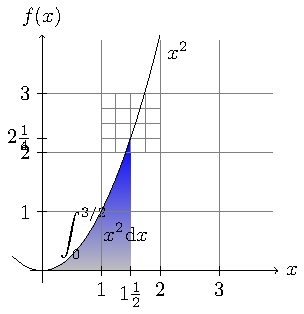
\includegraphics[width=0.7\linewidth]{mai_fig031.pdf}
    \caption{
            (\cite[s.~10000]{Feynman01})}
    \label{mai:fig031}
  \end{figure}

  \subsection{Výpočet integrálu}
      \begin{example}
        Spočítejme integrál $\displaystyle \int_1^{ln5}{(x+1)e^xdx}$  metodou per partes: 
        \begin{align*}
          \int{(x+1)e^xdx} &= \int{e^xdx}+\int{x\cdot e^xdx}
                            = e^x + (x-1)e^x = xe^x               \\
          \int_1^{ln5}{(x+1)e^xdx} &= [xe^x]_1^{ln5} = 5ln5-e     \\
        \end{align*}
        kde integrál
        \begin{equation*}
            \int{xe^xdx}=
              \left[\begin{array}{cc}
                u=x   & dv=e^x \\
                du=dx & v=e^x
              \end{array}\right]=
              xe^x-\int{e^xdx} = xe^x - e^x+C
        \end{equation*}
      \end{example}

\section{Vlastnosti určitého integrálu}
  V této kapitole mluvíme o spojitých funkcích $\Rightarrow$ příslušné integrály tedy vždy
  existují. Čerpáno z knih:
  \cite{Knichal}.

  \begin{lemma}
    \textbf{První věta o střední hodnotě integrálního počtu}: Je-li funkce $f(x)$ spojitá v
    intervalu $\langle a, b\rangle$, existuje alespoň jeden takový bod $c\in(a, b)$, že platí

    \begin{equation}\label{MA:eq_av1}
      \int_a^b f(x)dx = (b-a)f(c).
    \end{equation}
  \end{lemma}

  \begin{proof} Použitím Lagrangeovy věty napsané pro funkci $F(x)$, primitivní na intervalu
    $\langle a, b\rangle$ k dané funkci $f(x)$. Podmínky věty jsou zřejmě splněny: $F(x)$ je
    spojitá na intervalu $\langle a, b\rangle$ a má všude derivaci $F'(x)= f(x)$. Tedy existuje
    alespoň jeden bod $c\in(a, b)$,
    
    \begin{figure}[ht!]  %\ref{mai:fig029}
      \centering
      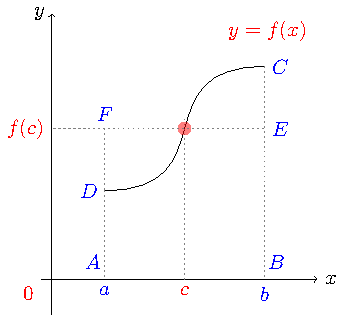
\includegraphics[width=0.7\linewidth]{mai_fig029.pdf}
      \caption{Vztah mezi silou tření a kolmou silou při smýkání
              (\cite[s.~173]{Feynman01})}
      \label{mai:fig029}
    \end{figure}

     že $$F(b)-F(a) = (b-a)F'(c),$$ čímž je věta dokázána, neboť $F(b)-F(a) = \int_a^bf(x)dx$ a
     $F'(c) = f(c)$. Funkční hodnotu $f(c)$, danou podle (\ref{MA:eq_av1}) rovnicí  
     \begin{equation}\label{MA:eq_av2}
        f(c) = \frac{1}{b-a}\int_a^b f(x)dx
     \end{equation}
     nazýváme \texttt{střední hodnotou}.
  \end{proof}

  Pro spojitou nezápornou funkci $f(x)$, lze větu o střední hodnotě jednoduše geometricky
  interpretovat dle (obr.\ref{mai:fig029}). Levá strana (\ref{MA:eq_av1}) určuje obsah
  křivočarého lichoběžníka $ABCD$, pravá strana obsah obdélníka $ABEF$. Podle této věty nabývá
  funkce $f(x)$ aspoň v jednom bodě intervalu $(a, b)$ takové hodnoty $f(c)$, že uvažovaný
  křivočarý lichoběžník má stejný obsah jako obdélník o základně $b-a$ a výšce $f(c)$ (str. 155
  knihy \cite{Knichal}).

      %---------------------------------------------------------------
      % !TeX spellcheck = cs_CZ
\begin{mdframed}[style=mdexam]
  \begin{example}\label{MAI:exam032}
    Určete střední hodnotu $i_s$ střídavého proudu $$i(t) = I_0\sin\omega t$$ v časovém intervalu
    $\langle 0, \frac{T}{2}\rangle$ (v průběhu jedné poloviny periody). $I_0$ je maximální hodnota
    proudu (obr. \ref{MAI:exam032}), perioda $T$ je dána vztahem $T = \frac{2\pi}{\omega}$
    
    {\centering
    \captionsetup{type=figure}
    \luafigure[1]{mai_fig030.pdf}
    \captionof{figure}{K příkladu \ref{MAI:exam032}
    \cite[s.~119]{Brabec1989}
    \label{mai:fig030}}
    \par}

      Podle \ref{MA:eq_av2} bude
      \begin{align*}
      i_s &=  \frac{2}{T}
              \int_0^{\frac{T}{2}}I_0\sin\omega t\dd{t} =
              \frac{2I_0}{T}\left[-\frac{\cos\omega t}{\omega}\right]_0^{\frac{T}{2}}        \\
          &=  \frac{2I_0}{T}\frac{1}{\omega}\left(-\cos\frac{\omega T}{2}+ \cos 0\right)     \\
          &=  \frac{2I_0}{2\pi}(-\cos\pi + \cos 0) = \frac{2}{\pi}I_0 \doteq 0,637 I_0.
    \end{align*}

    Tato hodnota se rovná intenzitě elektrického proudu, při kterém by vodičem v průběhu uvažované
    poloviny periody prošel stejný elektrický náboj jako při proudu střídavém.
  \end{example}
\end{mdframed}
















      %---------------------------------------------------------------

  \begin{example} Efektivní hodnota $i_{ef}$ střídavého proudu $$i(t) = I_0\sin\omega t$$ (viz
    předchozí příklad) je definována jako odmocnina ze střední hodnoty funkce $i^2(t)$ v průběhu
    jedné periody $T = \frac{2\pi}{\omega}$. Tedy
    \begin{align*}
      i_{ef}^2 &= \frac{1}{T}\int_0^T I_0^2\sin^2\omega t\dd{t} = 
                  \frac{1}{T}\int_0^T \frac{I_0^2}{2}(1- \cos2\omega t)\dd{t}           \\
               &= \frac{I_0^2}{2T}
                  \left[
                    t-\frac{\sin2\omega t}{2\omega}
                  \right]_0^T = \frac{I_0^2}{2}
    \end{align*}
    neboť $\sin2\omega T=\sin4\pi = 0.$ Odtud $$i_{ef} = \frac{I_0}{\sqrt{2}}.$$ Střídavý proud
    $i(t) = I_0\sin\omega t$ má na témže odporu stejný výkon jako stejnosměrný proud o intenzitě
    $i = 0,707I_0$.
  \end{example}
  Následující věta může být využita k odhadu některých integrálů
  \begin{lemma}
    \textbf{Druhá věta o střední hodnotě integrálního počtu}: Jsou-li funkce $f(x)$ a $g(x)$
    spojité v intervalu $\langle a, b \rangle$ a je-li funkce $g(x)$ v $\langle a, b \rangle$
    nezáporná a nerostoucí, existuje alespoň jeden bod $c\in\langle a, b \rangle$ tak, že platí
    \begin{equation}\label{MA_eq_av3}
        \int_a^b f(x)g(x) = g(a)\int_a^c f(x)dx.
    \end{equation}
  \end{lemma}
  Zcela obdobnou větu lze vyslovit pro případ, že $g(x)$ je v intervalu $\langle a, b \rangle$
  nezáporná a neklesající, tj. na pravé straně \ref{MA_eq_av3} je pak integrál $g(b)\int_c^b
  f(x)dx$

  \begin{example} Odhadněte hodnotu integrálu
    \begin{equation}\label{MA_eq_sinx_x}
        \int_{100\pi}^{1000\pi}\frac{\sin x}{x}dx
    \end{equation}
    Řešení: Funkce $f(x) = \sin x$ a $g(x) = \frac{1}{x}$ jsou v uvažovaném intervalu $\langle
    100\pi, 1000\pi \rangle$ spojité a funkce $g(x)$ je kladná a nerostoucí.
    \begin{equation*}
      \int_{100\pi}^{1000\pi}\frac{\sin x}{x}dx = 
      \frac{1}{100\pi}\int_{100\pi}^c\sin xdx =\frac{1}{100\pi}\left(\cos100\pi - \cos c\right)
    \end{equation*}
    kde $c$ je kladné číslo z intervalu $\langle 100\pi, 1000\pi \rangle$. Dále pro všechna
    $c\in\langle 100\pi, 1000\pi \rangle$ platí $0\leq1-\cos c\leq2$, takže
    \begin{equation*}
        0\leq\int_{100\pi}^{1000\pi}\frac{\sin x}{x}dx\leq \frac{1}{50\pi}.
    \end{equation*}
  \end{example}   

%} %tikzset
%---------------------------------------------------------------------------------------------------
\printbibliography[heading=subbibliography]
\addcontentsline{toc}{section}{Seznam literatury}
%  % !TeX spellcheck = cs_CZ
%{\tikzset{external/prefix={tikz/MAI/}}
% \tikzset{external/figure name/.add={ch04_}{}}
%---------------------------------------------------------------------------------------------------
% file: Theory_of_Derivates.tex
%---------------------------------------------------------------------------------------------------
\chapter{Derivace funkce}\label{mai:IchapIV}
\minitoc

%============== Kapitola: Derivace funkce ==========================================================
  \section{Základní věty diferenciálního počtu}
    \subsection{Věta o největší (nejmenší) hodnotě funkce}
      V tomto článku uvedeme významné věty, zvané souhrně věty o \emph{střední hodnotě 
      diferenciálního počtu}, a dále pak ukázky jejich užití v matematické analýze.  Avšak dříve 
      než budeme tyto věty formulovat, uvedeme jedno důležité tvrzení, které sice bude mít v 
      dalších úvahách tohoto článku pomocnou úlohu, ale v teorii extrémů má i samostatný význam. 
      \cite[s.~186]{Brabec1989} 
      \begin{lemma}\label{MA1:lem_diff02}
        Nechť funkce $f:A\rightarrow\realset$ nabývá na množině $A$ své největší (nejmenší) hodnoty 
        na vnitřním bodě $c$ množiny $A$. Máli funkce $f$ v bodě $c$ derivaci, potom $f'(c)=0$.  
      \end{lemma}
      \begin{proof}
        Nechť např. $f(c)$ je největší hodnota funkce $f$ na množině $A$, takže $f(x)\leq f(c)$ pro $\forall x\in A$. Potom pro $x\in A, x<c$, je 
        $$\frac{f(x)-f(c)}{x-c}\geq 0$$
        a tedy
        $$f'_{-}(c)=\lim_{x\rightarrow c^-}\frac{f(x)-f(c)}{x-c}\geq0$$ 
        Dále pro $x\in A, x>c$, je
        $$\frac{f(x)-f(c)}{x-c}\leq 0$$ 
        a proto
        $$f'_{+}(c)=\lim_{x\rightarrow c^+}\frac{f(x)-f(c)}{x-c}\leq0$$
        Platí tedy
        $$f'_{+}(c)\leq f'_{-}(c)\geq f'_{-}(c).$$ 
        Avšak $f'_{+}(c)=f'_{-}(c)= f'(c)$. Odtud plyne $f'(c)=0$. 
      \end{proof}
      
    \subsection{Věty o střední hodnotě}
      \begin{lemma}\label{MA1:lem_diff03}
        \textbf{Rolleova věta}\footnote{Michel Rolle [Mišel Rol] (1652-1719) Francouzský matematik} Nechť funkce $f$ má tyto vlastnosti:
          \begin{enumerate}
            \item je spojitá na uzavřeném intervalu $\langle a,b\rangle$;
            \item má derivaci (vlastní či nevlastní) na otevřeném intervalu $(a,b)$;
            \item platí $f(a)=f(b)$.
          \end{enumerate}
        Potom v otevřeném intervalu $(a,b)$ existuje aspoň jeden bod $\xi$ takový, že $f'(\xi)=0$.   
      \end{lemma}
      \begin{proof}
        Protože je funkce $f$ je na uzavřeném intervalu $\langle a,b\rangle$ spojitá, nabývá v 
        tomto intervalu své největší hodnoty $M$,své nejmenší hodnoty $m$. Přitom ovšem platí:
        \begin{equation}\label{MA1:eq_diff02}
          m\leq f(x) \leq M, \qquad x\in\langle a,b\rangle.
        \end{equation}
        Nyní mohou nastat dva případy: 
        \begin{enumerate}
          \item funkce $f$ nabývá $M$ i $m$ právě v krajních bodech intervalu $\langle a,b\rangle$. Podle předpokladu 3 věty \ref{MA1:lem_diff03}
                však potom platí $f(a)=f(b)=m=M$. Vzhledem ke vztahu \ref{MA1:eq_diff02} odtud plyne, že funkce $f$ je konstantní na intervalu
                $\langle a,b\rangle$ a tedy $f'(x)=0$ dokonce v každém bodě $x\in(a,b)$
          \item Funkce $f$ nabývá apsoň jedné z hodnot $M$, $m$ v některém vnitřním bodě $\xi$ intervalu $\langle a,b\rangle$. Potom podle 
          věty \ref{MA1:lem_diff02} je $f'(\xi)=0$.         
        \end{enumerate}        
      \end{proof}
      \begin{note}
        Rolleova věta sama zaručuje jen existenci aspoň jednoho bodu $\xi\in(a,b)$, ve kterém je fe 
        $f'(\xi)=0$. Neumožňuje však ani určení tohoto bodu (nebo bodů), ani stanovení jejich počtu 
      \end{note}
      
      \begin{note}
        Na obr. \ref{MAI:fig_027} je ilustrován geometrický význam Rolleovy věty. Graf funkce na 
        tomto obrázku má v bodech $\xi_1$, $\xi_2$, v nichž je $f'(\xi_1)=f'(\xi_2)=0$ tečny 
        rovnoběžné s osou $x$. 
        \begin{figure}[ht!] %\ref{MAI:fig_027}
          \centering
          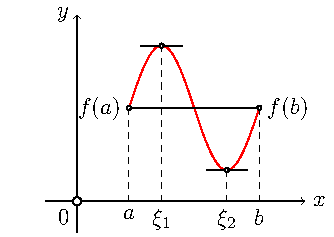
\includegraphics[width=0.7\linewidth]{mai_fig027.pdf}
          \caption{K výkladu Rolleovy věty}
          \label{MAI:fig_027}
        \end{figure}
      \end{note}
      
      Z Rolleovy věty plyne důležitá věta:
      
      \begin{lemma}\label{MA1:lem_diff04}
        (\textbf{Cauchyova věta}). Nechť funkce $f$ a $g$ mají tyto vlastnosti:
        \begin{enumerate}
          \item  Jsou spojité na uzavřeném intervalu $\langle a,b\rangle$,
          \item  v každém bodě $x\in(a,b)$ existuje derivace $f'(x)$ (vlastní či nevlastní) a vlastní derivace $g'(x)$,
          \item  $g'(x)\neq0$ na $(a,b)$
        \end{enumerate}
        Potom v otevřeném intervalu $(a,b)$ existuje aspoň jeden bod $\xi$, pro který platí
        \begin{equation}\label{MA1:eq_diff03}
          \frac{f(b)-f(a)}{g(b)-g(a)} = \frac{f'(\xi)}{g'(\xi)}.
        \end{equation} 
      \end{lemma} 
      
      \begin{proof}
        Poznamenejme především, že z předpokladu 3 $g'(x)\neq0$ pro $x\in(a,b)$ a z předpokladu 
        spojitosti funkce $g$ na uzavřeném intervalu $\langle a,b\rangle$ ihned vyplývá vztah 
        $g(b)- g(a)\neq 0$. Kdyby totiž bylo $g(b)=g(a)$, potom by podle \emph{Rolleovy věty} 
        \ref{MA1:lem_diff03} existoval aspoň jeden bod $\eta\in(a,b)$ takový že $g'(\eta)=0$. To 
        však by byl spor s předpokladem $g'(x)\neq0$ pro každý bod $x\in(a,b)$. Proto má smysl 
        podíl na levé straně rovnosti \ref{MA1:eq_diff03}
        
        K vlastnímu důkazu Cauchyovy věty zavedeme takovou pomocnou funkci $F$, aby splňovala podmínky Rolleovy věty. Definujme ji pro $x\in\langle a,b\rangle$ předpisem
        \begin{equation}\label{MA1:eq_diff04}
          F(x)=[f(b)-f(a)]\cdot[g(x)-g(a)]-[f(x)-f(a)]\cdot[g(b)-g(a)].
        \end{equation}
        Snadno ověříme, že tato funkce skutečně splňuje podmínky Rolleovy věty na intervalu $\langle a,b\rangle$:
        \begin{itemize}
          \item Je spojitá na intervalu $x\in\langle a,b\rangle$, což je důsledkem spojitosti  
                funkce $f$ a $g$ na intervalu $x\in\langle a,b\rangle$ ,
          \item má derivaci $F'$ na otevřeném intervalu $(a,b)$, což plyne z existence derivace  
                $f'$ a $g'$ funkce $f$ a $g$ na  intervalu $(a,b)$,
          \item $F(a)=F(b)=0$ 
        \end{itemize}
        Platí tedy i závěr Rolleovy věty pro funkci $F$, tj. na intervalu $(a,b)$ existuje aspoň 
        jeden bod $\xi$, pro který $F'(\xi)=0$. Zderivujeme-li funkci $F$, dostaneme (dosadíme-li 
        $x=\xi$): $$F'(\xi)=[f(b)-f(a)]g'(\xi)-f'(\xi)[g(b)-g(a)]=0$$ Odtud již plyne rovnost 
        \ref{MA1:eq_diff03}                  
      \end{proof}
      
      Významným zvláštním případem Cauchyovy věty je další věta, která se častěji používá.
      
      \begin{lemma}\label{MA1:lem_diff05}
        (\textbf{Lagrangeova věta})\footnote{Joseph Louis Lagrange [lagránž] (1736-1813), francouzský matematik}. Nechť funkce má tyto vlastnosti:
        \begin{itemize}
          \item Je spojitá na intervalu $\langle a,b\rangle$,
          \item má derivaci (vlastní či nevlastní) na otevřeném intervalu $(a,b)$. 
        \end{itemize} 
        Potom existuje v otevřeném intervalu $(a,b)$ aspoň jeden bod $\xi$, pro který platí 
        \begin{equation}\label{MA1:eq_diff05}
           \frac{f(b) - f(a)}{b - a} = f'(\xi),  
        \end{equation}  
        či-li
        \begin{equation}\label{MA1:eq_diff06}
           f(b) - f(a) = f'(\xi)(b-a),  
        \end{equation}           
      \end{lemma}
      
      \begin{proof}
        Tvrzení této věty je důsledkem tvrzení \emph{Cauchyovy věty}, a to pro případ $g(x)=x$. 
        Protože $g'(x)=1$ dokonce všude, jsou splněny všechny tři podmínky Cauchyovy věty. Proto 
        platí i závěr této věty, z něhož pro náš případ již plyne vzorec \ref{MA1:eq_diff05} a tedy 
        i vzorec \ref{MA1:eq_diff06}.  
      \end{proof}
      
      \begin{note}
        Podobně jako je Lagrangeova věta zvláštním případem věty Cauchyovy, je Rolleova věta zvláštním případem Lagrangeovy věty, a to přo případ, že $f(a)=f(b)$.
      \end{note}
      
      \begin{note}
        Lagrangeova věta se často nazývá \emph{větou o přírůstku funkce}, protože vzorcem \ref{MA1:eq_diff06} se vyjadřuje \emph{přírůstek funkce}, tj rozdíl $f(b)-f(a)$. 
        Všechny tři uvedené věty, tj. věta Rolleova, Cauchyova a Lagrangeova, se v literatuře nazývá souhrně \textbf{věty o střední hodnotě diferenciálního počtu}.
      \end{note}
      
      \begin{note}
        Na obr. ** je ilustrován geometrický význam Lagrangeovy věty. Podíl na levé straně rovnosti 
        \ref{MA1:eq_diff05}, tj. číslo $\frac{f(b) - f(a)}{b - a}$ je směrnice sečny $s$, spojující 
        body $A$, $B$ grafu funkce  $f$, které odpovídají krajním bodům intervalu $\langle 
        a,b\rangle$. Podle tvrzení Lagrangeovy věty existuje v otevřeném intervalu $(a,b)$ aspoň 
        jeden bod $\xi$ tak, že tečna grafu funkce $f$ v příslušném jeho bodě je rovnoběžná s 
        přímkou $s$.  
      \end{note}
      
      \begin{note}
        Z Lagrangeovy věty vyplývá toto tvrzení: Nechť funkce $f$ vyhovuje na intervalu $\langle a,b\rangle$ podmínkám Lagrangeovy věty a $x_1$, $x_2$ jsou dva libovolné různé body
        intervalu $\langle a,b\rangle$. Potom v otevřeném intervalu s krajnímy body $x_1$, $x_2$ existuje aspoň jeden bod $\xi$, pro který platí Lagrangeův vzorec:   
        \begin{align}
          f(x_2) - f(x_1)                  &= f'(\xi)(x_2-x_1) \label{MA1:eq_diff07} \\ 
          \frac{f(x_2) - f(x_1)}{x_2-x_1}  &= f'(\xi)          \label{MA1:eq_diff08}      
        \end{align}
        Potom bod $\xi$ lze vyjádřit takto:
        \begin{equation}\label{MA1:eq_diff09}  
          \xi = x_1 + \vartheta(x_2-x_1), \qquad \text{kde }\vartheta\in(0,1). 
        \end{equation}
        Označíme-li $x_2-x_1=h$, můžeme vzorec \ref{MA1:eq_diff07} napsat ve tvaru
        \begin{equation}
          f(x_1+h) - f(x_1)= f'(x_1 + \vartheta h)h, \qquad \text{kde }\vartheta\in(0,1). 
        \end{equation} 
      \end{note}       
          
    \subsection{Některé důsledky Lagrangeovy věty}
      Lagrangeova věta, má některé významné důsledky, které nyní uvedeme \cite[s.~189]{Brabec1989}:
      \begin{lemma}\label{MA1:lem_diff06} 
        Nechť funkce $f$ vyhovuje podmínkám Lagrangeovy věty a navíc nechť $f'(x)=0$ pro všechna 
        $x\in(a,b)$. Potom funkce $f$ je prostá na intervalu $\langle a,b \rangle$. 
      \end{lemma}
      \begin{proof}
        Necť $x_1, x_2$ jsou libovolné dva různé body intervalu $\langle a,b \rangle$. Potom podle 
        Lagrangeova vzorce \ref{MA1:eq_diff04} platí 
        \begin{equation}
          f(x_2) - f(x_1) = f'(\xi)(x_2-x_1) \neq0
        \end{equation}
        neboť $f'(\xi)\neq 0$ dle předpokladu.
      \end{proof}
      
      \begin{lemma}\label{MA1:lem_diff01}
        Funkce $f$ je konstantní na intervalu $(a,b)$, právě když má na tomto intervalu derivaci a platí $f'(x) = 0$ pro všechna $x\in(a,b)$. 
      \end{lemma}
      \begin{proof} Tedy
        \begin{itemize}
          \item Je-li funkce $f$ konstantní na intervalu $(a,b)$, pak je $f'(x) = 0$ pro všechna  
                $x\in(a,b)$, jak již víme.
          \item Nechť $f'(x) = 0$ pro všechna $x\in(a,b)$. Dokažme, že pro každé dva body $x_1, 
                x_2  \in(a,b)$, $x_1\neq x_2$, platí $f(x_1) = f(x_2)$. Z existence
                derivace vyplývá spojitost funkce a jsou tedy splněny podmínky Lagrangeovy věty na 
                každém intervalu $\langle x_1, x_2\rangle\subset(a,b)$. Podle vzorce 
                \ref{MA1:eq_diff04} tedy platí $f(x_2)-f(x_1)f'(\xi)(x_2-x_1)$, $\xi\in(x_1,x_2)$. 
                Protože podle předpokladu je $f'(x)=0$ pro $\forall x\in(a,b)$, platí $f(x_1) 
                -f(x_2)=0$, tj. $f(x_1)=f(x_2)$  
        \end{itemize}
      \end{proof}
      
%} % tikzset
%---------------------------------------------------------------------------------------------------
\printbibliography[heading=subbibliography]
\addcontentsline{toc}{section}{Seznam literatury}
%  % !TeX spellcheck = cs_CZ
%{\tikzset{external/prefix={tikz/MAI/}}
% \tikzset{external/figure name/.add={ch05_}{}}
%---------------------------------------------------------------------------------------------------
% file: Differential_Calculus_applications.tex
%---------------------------------------------------------------------------------------------------
\chapter{Aplikace diferenciálního počtu}\label{chap:Apl_dif_poc}
\minitoc

%================Kapitola: Aplikace diferenciálního počtu =========================================
Diferenciální počet má rozsáhlou oblast užití. V této kapitole ukážeme použití výsledků předchozích 
kapitol k vyšetřování průběhu funkce a vlastnosti rovinných křivek. 
  \section{Průběh funkce}
    Pomocí derivace můžeme studovat vlastnosti funkce, které usnadní vyšetřování jejího průběhu.  
    \subsection{Monotonie funkcí}
      Jednou z důležitých vlastností funkce je její \textquotedblleft monotonie\textquotedblright, 
      kterou jsme definovali již v odst. \ref{MA1:subsec_vlastnosti_funkce} kap. 
      \ref{mai:IchapLimit}. Proto je při vyšetřování průběhu funkce důležité určit množiny (často 
      jsou to intervaly), na nichž je funkce monotónní, jinak řečeno, najít \textquotedblleft 
      intervaly monotonie funkce\textquotedblright (viz \cite[s.~208]{Brabec1989}). 
    \begin{enumerate}
      \item Zjistíme \textbf{definiční obor funkce}, vyjádříme jej v intervalech a z nich poznáme,  
            kde je funkce \textbf{spojitá}. Funkce je spojitá v $(a,b)$ pro každý bod tohoto 
            intervalu, když$|f(x)-f(c)|<\varepsilon$, kde $\varepsilon>0$ je libovolně zvolené 
            číslo, a pro všechna $x$ z okolí bodu $c$ je $|x-c|<\delta$, kde $\delta>0$ je na 
            $\varepsilon$ nezávislé.
      \item Určíme, je-li funkce \textbf{lichá} $f(-x)=-f(x)$ nebo \textbf{sudá} $f(-x)=f(x)$.   
            Je-li funkce lichá, je souměrná podle středu souměrnosti (obyčejně to bývá počátek 
            souřadnic $xy$), je-li sudá, je souměrná podle osy $y$.
      \item Určíme \emph{průsečíky křivky s osami pravoúhlých souřadnic}. Body, ve kte\-rých 
            křivka  protíná osu $x$ spolu s body, ve kte\-rých není křivka spojitá, rozlišují 
            intervaly, v nichž je graf křivky nad osou $x$ od intervalů, ve kterých je graf křivky 
            pod osou $x$.
      \item V krajních bodech definičních intervalů, ve kterých je funkce spojitá, stano\-víme 
      \emph{limity funkce} a dále $$\lim_{x \to \pm \infty}f(x).$$
      \item Vypočítáme $f'(x)$ a $f''(x)$, abychom zjistily, kde je funkce \emph{rostoucí}     
            $f'(x)>0$, \emph{klesající} $f'(x)<0$ a kde jsou \emph{lokální extrémy}. Dostaneme-li 
            dosazením kořenů rovnice $f'(x)=0$ do $f''(x)$ hodnotu $f''(x)>0$, má funkce lokální 
            minimum, při $f''(x)<0$ má funkce lokální maximum. V intervalech, kde $f''(x)>0$, je 
            křivka \textbf{konvexní (vypuklá)}, kde $f''(x)<0$, je křivka \textbf{konkávní 
            (vydutá)}. Body, v nichž $f''(x)$ mění znaménko, jsou \textbf{inflexní body}. Najdeme 
            je tak, že stanovíme hodnoty $x$, pro které je $f''(x)=0$ nebo neexistuje. Číslo $c$ je 
            inflexní bod, když existuje takové okolí bodu $c$, že pro $x>c$ je oblouk křivky 
            konvexní a pro $x<c$ konkávní. Je nutné si uvědomit, že když má $f'(x)$ konečnou 
            derivaci, je inflexní bod $c$ taky nulovým bodem druhé derivace čili kořenem rovnice 
            $f''(x)=0$. Obrácená věta neplatí, tj. z $f''(x)=0$ nevyplývá, že v bodě $c$ má $f'(x)$ 
            extrém a že bod $c$ je inflexním bodem.
      \item \textbf{Asymptota} je tečna křivky $f(x)$, jejíž bod dotyku je v nekonečnu. Platí-li  
            $$\lim_{x \to a}f(x) =  \pm\infty,$$ je přímka $x=a$ její asymptotou. Jinak asymptoty 
            mají rovnici $y=kx+q$, kde $x$ a $y$ jsou souřadnice bodů na asymptotách. Existují-li 
            konečné limity $$\lim_{x \to \pm\infty}\frac{f(x)}{x}=k$$  a $$\lim_{x \to 
            \pm\infty}[f(x)-kx] =q$$ pak je asymptotou přímka $y=kx+q$. Můžeme-li rovnici křivky 
            rozložit (tj. rozložit její pravou stranu, oby\-čejně dělením čitatele jmenovatelem, 
            má-li tvar zlomku) na dvě části, z nichž jedna má tvar $kx+q$ a druhá zbytek 
            $\varphi(x)$, tj. $f(x)=kx+q+\varphi(x)$ a $\varphi(x)_{x\rightarrow 
            \pm\infty}\rightarrow 0$, je přímka $y=kx+q$ asymptotou.
      \item Zpřesnění grafu křivky provedeme sestavením tabulky souřadnic dalších bodů křivky,  
            tj. ke zvoleným hodnotám $x$ (z definičního oboru funkce) vypočítáme hodnoty $y$. Do 
            dalších řádků tabulky zapíšeme hodnoty  $f'(x)$ a $f''(x)$, ve kterých intervalech je 
            funkce \emph{rostoucí}, ve kterých \emph{klesá}, kde je \emph{vypuklá}, kde je 
            \emph{dutá}, kde jsou \emph{lokální extrémy}, \emph{inflexní body} apod., 
            případně sestavíme dílčí tabulky pro jednotlivé \emph{charakteristické vlastnosti} vyšetřované funkce.
    \end{enumerate}
    %-------------------- EXAM001 --------------------------------------
    % !TeX spellcheck = cs_CZ
\begin{mathexam}{Vyšetřete průběh funkce \(f(x):y=\frac{1+x^2}{1-x^2}\)}{exam003}
  \begin{enumerate}[noitemsep]
    \item Definiční obor $D_f=\realset-\{±1\}=(-\infty,-1)\cup(-1,1)\cup(1,+\infty)$
    \item Funkce je sudá $$f(-x)=f(x): \frac{1+x^2}{1-x^2}=\frac{1+(-x)^2}{1-(-x)^2}.$$ Funkce není
        periodická.
    \item Stanovíme funkční hodnoty v krajních bodech definičního obor $1, -1$ a v nevlastních
        bodech $-\infty,+\infty$.Protože je funkce \textbf{sudá}, omezíme se jen na vyšetřování
        nezáporné části. Nejprve vlastnosti funkce v okolí bodu $1$. Ten nepatří do $D_f$ a proto
        určíme limity funkce v pravém a levém okolí tohoto bodu. $$\lim_{x\to
        1_{-}}=\frac{1+x^2}{1-x^2}.$$ Pro výpočet limity použijeme substituci $y=1-x^2$: 
        $$\lim_{y\to0+}\frac{2-y}{y}=+\infty$$ \footnote{$\lim_{x\to0_+}\frac{1}{x}=\infty$} proto
        
        $$\lim_{x\to1_{-}}\frac{1+x^2}{1-x^2}=+\infty.$$ Obdobně dojdeme k
        $$\lim_{x\to1_+}\frac{1+x^2}{1-x^2}=-\infty.$$ A konečně v nevlastních bodech $±\infty$ je
        limita $$\lim_{x\to±\infty}\frac{1+x^2}{1-x^2} = \lim_{x\to\pm\infty}\frac{1}{1-x^2} +
        \lim_{x\to\pm\infty}\frac{x^2}{1-x^2}=0-1=-1.$$ Výpočtem limit jsme zároveň určili dva
        absolutní (globální) extrémy a jeden lokální:
        \begin{itemize}
          \item v intervalu $(-1,1)$ má funkce maximum $\infty$ a minimum $1$,
          \item v intervalech $(-1,1)\cup(1,+\infty)$ má funkce minimum $-\infty$ a maximum $-1$.
        \end{itemize}
    \item Nyní vyšetříme zda, případně kolik a jaké, má funkce $f(x)$ průsečíky s osami souřadnic. S
        osou $x$ nemá funkce žádné průsečíky, protože pro $y=0$ není definována
        $H_f=\realset-\{-1,1\rangle$. Pro $x=0$ je $y=\frac{1+0^2}{1-0^2}=1$, proto má $f(x)$ právě
        jeden průsečík s osou $y$ a to $[0,1]$.
    \item Zatím jsme zjistili, že naše funkce není definována v bodech $1$ a $-1$ a proto není
        spojitá v  $\realset$. Nevíme však, jaký je její průběh v jednotlivých intervalech
        definičního oboru.  Abychom získali názornější představu o průběhu funkce, zjistíme má-li
        derivaci.
        \begin{align*}
          y' &= \frac{(1+x^2)'(1-x^2 )-(1+x^2)(1-x^2 )'}{(1-x^2)^2} \\
          y' &= \frac{2x(1-x^2 )-(1+x^2 )(-2x)}{(1-x^2 )^2}         \\
          y' &= \frac{4x}{(1-x^2 )^2}
        \end{align*}
        Protože má vlastní derivaci\footnote{$f(x)$ je spojitá v intervalech $(-\infty,-1),
        (-1,1),(1,\infty)$  věta s spojité funkci}, můžeme určit její vlastnosti v intervalech
        $\langle0,1)$ a $(1,\infty)$. V těchto intervalech je $y'>0$ a proto jde o funkci ryze
        monotónní, rostoucí \footnote{Plyne z věty o postačujících podmínkách ryzí monotónnosti
        funkce na intervalu} v daných intervalech \footnote{V intervalech
        $(-\infty,-1),(-1,0\rangle$ je funkce klesající.}. Výpočtem zjistíme druhou derivaci funkce.
        Ta nám pomůže určit další extrém v intervalu $\langle0,1)$ a zároveň vyšetřit
        \textbf{konkávnost} a \textbf{konvexnost}.
        \begin{align*}
          y'' &= \frac{(4x)' (1-x^2 )^2-(4x)(1-2x^2+x^4 )'}{(1-x^2 )^4}  \\
          y'' &= \frac{4(1-2x^2+x^4 )-4x(-4x+4x^3 )}{(1-x^2 )^4}         \\
          y'' &= \frac{4(1-x^2 )(3x^2+1)}{(1-x^2 )^4}                    \\
          y'' &= \frac{4(3x^2+1)}{(1-x^2 )^3}
        \end{align*}
        Abychom mohli určit lokální extrém funkce $f(x)$ v intervalu $\langle0,1)$, pomocí druhé
        derivace, musíme najít kořeny rovnice $f' (x)=0$. V našem případě
        $$y'=\frac{4x}{(1-x^2)^2}\Rightarrow\frac{4x}{(1-x^2)^2}=0\rightarrow x_0=0,$$ tento kořen
        \footnote{stacionární bod}  pak dosadíme do druhé derivace, tj. 
        $$y''(0)=\frac{4(3\cdot0^2+1)}{(1-0^2 )^3}=4,$$ protože je $f''(x)>0$, má v bodě $x_0$
        lokální minimum. Můžeme rovněž konstatovat, že funkce nemá inflexní body \footnote{Pro
        existenci inflexního bodu je nutné splnění jedné z podmínek a to buď $f''(x_0)=0$, nebo
        $f''(x_0)$ neexistuje.}. Konkávnost a konvexnost funkce v intervalech $\langle0,1)$ a
        $(1,\infty)$ vyšetříme pomocí vlastností druhé derivace funkce. Tedy
        \begin{itemize}
          \item $\langle0,1): y''=\frac{4(3x^2+1)}{(1-x^2 )^3} >0 \Rightarrow$ funkce je v tomto
                intervalu \textbf{konvexní},
          \item $(1,\infty): y''=\frac{4(3x^2+1)}{(1-x^2 )^3} <0 \Rightarrow$ funkce je v tomto
                intervalu \textbf{konkáv\-ní}.
        \end{itemize}
    \item Z předchozích výpočtů plyne, že křivka má asymptoty $y=-1,x=\pm1$.
  \end{enumerate}
  {\centering \captionsetup{type=figure}          % %\ref{MAI:fig_028}
    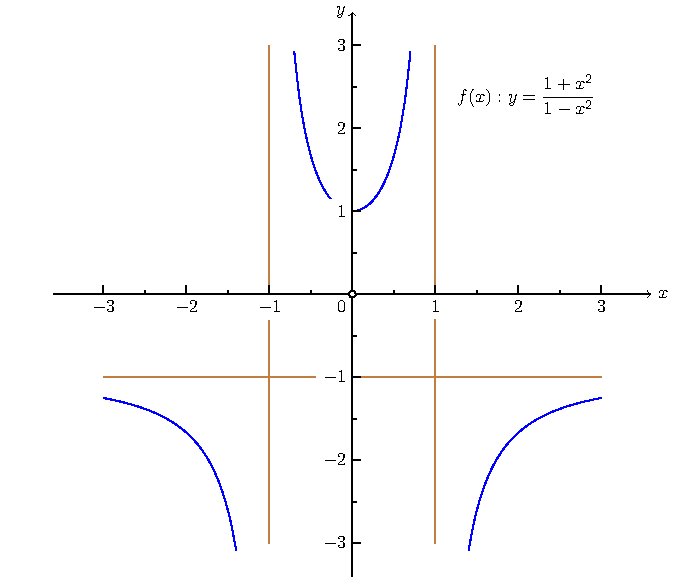
\includegraphics[width=1\linewidth]{mai_fig028.pdf}
    \captionof{figure}{Graf funkce $f(x):y=\dfrac{1+x^2}{1-x^2}$}
    \label{MAI:fig_028}
  \par}
\end{mathexam}  
    %-------------------------------------------------------------------

%} %tikzset
%---------------------------------------------------------------------------------------------------
\printbibliography[heading=subbibliography]
\addcontentsline{toc}{section}{Seznam literatury} 
%  % !TeX spellcheck = cs_CZ
%{\tikzset{external/prefix={tikz/MAI/}}
% \tikzset{external/figure name/.add={ch06_}{}}
%---------------------------------------------------------------------------------------------------
% file: chap_PrimitiveFce.tex
%---------------------------------------------------------------------------------------------------
%============================ Primitivní funkce ====================================================
\chapter{Primitivní funkce}
\minitoc

  %----------------------------Neurčitý integrál----------------------------------------------------
  \section{Motivace}
    Problém \emph{neurčitého integrálu}, neboli \textbf{primitivní funkce}, lze vyložit velmi 
    jednoduše: Máme podezření, že zadaná funkce \(f(x)\) vznikla derivováním jisté, zatím neznámé, 
    funkce \(F(x)\). Dokážeme ji najít? 
  
    K danému problému můžeme přistupovat také fyzikálně: Zavedením pojmu derivace funkce jsme 
    motivovali důležitým požadavkem definovat okamžitou rychlost pohybu bodu po přímce. Existuje 
    přirozeně i požadavek opačný, tj. nalézt zákon dráhy pohybu bodu po přímce, je-li dána jeho 
    okamžitá rychlost jako funkce času \cite[s.~253]{Brabec1989}. Vše si ukážeme na následujícím 
    příkladu:  
   
    \begin{example}
      Je dána okamžitá rychlost $v$ pohybu bodu po přímce (ose) $x$ rovnicí $v(t) = 2t + 1$, 
      $t\in\langle -\infty,+\infty \rangle$. Najděte zákon dráhy pohybu, je-li známo, že v čase $t 
      = 0$ měl bod polohu $x = x_0$.
      \newline
      \textbf{řešení:}\newline
      Označíme-li $x(t)$ polohu bodu v okamžiku $t$, pak $v(t) = \frac{dx}{dt}$. Hledáme tedy 
      funkci $x = x(t)$, pro níž platí 
      \begin{align}
        \frac{dx}{dt} &= 2t + 1 \qquad x(0) = x_0.  \nonumber \\ 
        \shortintertext{Je ihned patrné, že první podmínce vyhovuje nekonečně mnoho funkcí}
        x(t)          &= t^2 + t + C,           \label{MA:int_ex_09}    \\ 
        \shortintertext{ kde $C$ je libovolná konstanta. Funkce, která splňuje i druhou podmínku 
          (říkáme ji též počáteční podmínka), najdeme z rovnice \ref{MA:int_ex_09} dosazením dané podmínky 
          $t = 0,\ x = x_0$. Dostaneme $x_0 = C$. Dosazením do \ref{MA:int_ex_09} za $C$ plyne hledaný 
          zákon dráhy}
        x(t)          &= t^2+t+x_0.                 \nonumber 
        \shortintertext{Jednoduchou zkouškou se přesvědčíme, že tato funkce splňuje obě dané podmínky a 
          zároveň vidíme, že hledaná primitivní funkce daných vlastností je jediná.}  \nonumber
      \end{align}
    \end{example} 
    Každé takové funkci, jejíž derivací je daná funkce, budeme říkat \emph{primitivní funkce} k 
    dané funkci. Na uvedeném příkladě je patrné, že k dané funkci může existovat nekonečně mnoho 
    primitivních funkcí. Množinu všech primitivních funkcí se často nazývá \textbf{neurčitým 
    integrálem}. Po tomto názorném uvedení do problému přejděme k přesné formulaci základních pojmů.
    
    \begin{definition} 
      Funkce $F: J\rightarrow \realset$, kde $J\subset \realset$ je interval, se nazývá primitivní 
      funkce k funkci \(f\) na intervalu \(J\) právě když, pro všechna $x\in J$ je $F'(x) = f(x)$ 
      (v krajních bodech intervalu \(J\), pokud k němu patří, jde o derivace jednostranné).
    \end{definition}
    
    \begin{example} 
      K funkci $\sin x$ je primitivní funkcí na libovolném intervalu $J\subset(-\infty,+\infty)$ 
      funkce $-\cos x$, protože $(-\cos x)' = \sin x$. Ale též funkce $3-\cos x$ je primitivní 
      funkcí k funkci $\sin x$, protože $(3 - \cos x)' = \sin x$ pro všechna $x\in(-\infty, 
      \infty)$.
    \end{example}
    
    Je vidět, že rozdíl dvou primitivních funkcí k téže funkci je konstanta. To není náhoda, jak 
    potvrzuje následující věta:
    
    \begin{lemma}
      \begin{enumerate}
        \item Je-li funkce $F$ primitivní funkcí k funkci \(f\) na intervalu \(J\) a \(c\) reálná  
              konstanta, pak i funkce $G = F + c$ je primitivní funkcí k funkci \(f\) na intervalu 
              \(J\).
        \item Jsou-li funkce $F$ a $G$ primitivní funkce k funkci \(f\) na intervalu \(J\), pak 
        funkce
              $F-G$ je na intervalu \(J\) konstantní.
      \end{enumerate} 
      \begin{proof}
        Tvrzení a) plyne z definice protože $G'(x) = [F(x) + c] = F'(x) = f(x)$ pro všechna $x\in
        J$. Tvrzení b) je důsledkem věty \ref{MA1:lem_diff01}.
      \end{proof}
    \end{lemma}
    Neurčitost vyplývá právě z toho, že primitivní funkce není dána jednoznačně, je určena až na 
    konstantu. Značíme
    \begin{equation*}
      \boxed{F(x) = \int f(x)\dx + C}
    \end{equation*}
        
    Jak ale primitivní funkce hledat? V jednoduchých příkladech poslouží tabulka derivací, již 
    čteme „zprava doleva“. (Je dobré si ji uložit do paměti.) Tabulka však pokryje jen velmi málo 
    případů, pouze elementární funkce. Je tedy třeba najít metody, jak při hledání primitivních 
    funkcí postupovat. Nejprve však uvedeme dvě základní pravidla pro primitivní funkce, která 
    plynou z pravidel pro derivování:
    \begin{align}
      \int[f(x)\pm g(x)]\dx &= \int[f(x)\pm g(x)]\dx + \int[f(x)\pm g(x)]\dx \label{MA1:eq_int10} \\
      \int cf(x)\dx         &= c \int f(x)\dx, \qquad \text{\(c\) je konstanta.} \label{MA1:eq_int11}
    \end{align}
  
  \section{Tabulka neurčitých integrálů}\label{MA:chap_tabINT}
    Pokud není nic uvedeno, platí vzorce pro všechna \(x\) a pro všechny hodnoty uvedených
    konstant. Místo platí pro \(x\) z intervalu \((-\infty,0),(0,+\infty)\) píšeme stručně
    \(x\neq0\) apod. Literatura: \cite[p.~396]{Rektorys1963}.
  
    \begin{flalign}
      & \int 0\dx = c                                        &         \label{MA:baseInt01}     \\
      & \int a\dx = ax+c                                     &         \label{MA:baseInt02}     \\
      & \int x^n\dx = \frac{x^{n+1}}{n+1}+c, \,              &         \label{MA:baseInt03}     \\
      & \qquad\text{kde}\begin{cases}
          \forall x\in\realset,\,n\in\naturalset, n>0,         \\
          \forall x\in\realset-\{0\},\,n\in\naturalset, n<-1,  \\
          \forall x>0,\,n\in\realset\,\,n\notin\naturalset
        \end{cases}                                          &         \nonumber               \\
      & \int\frac{1}{x}\dx = 
            \ln\abs{x}+c \hspace{1ex}\forall x\neq0          &         \label{MA:baseInt04}     \\
      & \int e^x \dx       = e^x+c                           &         \label{MA:baseInt05}     \\
      & \int\ln x\dx       = 
          x\ln x - x + c \hspace{1ex}\forall x>0             &         \label{MA:baseInt06}     \\
      & \int a^x \dx     =
          \frac{a^x}{\ln a}+c 
          \hspace{1ex}\forall a>0,\,a\neq1                   &         \label{MA:baseInt07}     \\
      & \int \sin x \dx  = -\cos x                           &         \label{MA:baseInt08}     \\
      & \int \cos x \dx  =  \sin x                           &         \label{MA:baseInt09}     \\
      & \int\frac{1}{\cos^2x}\dx =  \tan x+c 
           \hspace{1ex}\forall x\neq(2k+1)\pi,\,k\in\naturalset &      \label{MA:baseInt10}     \\ 
      & \int\frac{1}{\sin^2x}\dx     =  -\cotg x+c
         \hspace{1ex}\forall x\neq k\pi,\,k\in\naturalset    &         \label{MA:baseInt11}     \\
      & \int\frac{1}{\sqrt{1-x^2}}\dx =
          \begin{cases}
            +\arcsin x + c         \\
            -\arccos x + c
          \end{cases} 
          \forall x\in(-1,1)                                 &         \label{MA:baseInt12}     \\
      & \int\cosh\dx = \sinh x + c                           &         \label{MA:baseInt13}     \\
      & \int\sinh\dx = \cosh x + c                           &         \label{MA:baseInt14}     \\
      & \int\frac{1}{1+x^2}\dx = \arctan x + c               &         \label{MA:baseInt15}     \\
      & \int \frac{1}{\sqrt{x^2 + 1}}\dx =
          \begin{cases}
            \ln(x + \sqrt{x^2+1}) + c         \\
            \sinh^{-1}x + c 
          \end{cases}                                        &         \label{MA:baseInt16}     \\ 
      & \int \frac{1}{\sqrt{x^2 - 1}}\dx =
          \begin{cases}
            \ln(x + \sqrt{x^2-1}) + c         \\
            \cosh^{-1}x + c \hspace{4ex}x\in(1,+\infty) 
          \end{cases}                                        &         \label{MA:baseInt17}     \\
      & \int\frac{1}{\sqrt{x^2+a^2}}\dx 
        = \sinh^{-1} \frac{x}{a} = \ln (x+\sqrt{x^2+a^2})    &         \label{MA:baseInt18}     \\
      & \int \frac{1}{\sqrt{x^2-a^2}}\dx 
        = \cosh^{-1} \frac{x}{a} = \ln (x+\sqrt{x^2-a^2})    &         \label{MA:baseInt19}     \\
      & \int\frac{1}{\sqrt{x^2-1}}\dx 
        = \left\{ 
          \begin{array}{l l}
            \ln\abs{x+\sqrt{x^2-1}}+c      &  \abs{x}>1  \\
            \cosh^{-1}x+c                  &  \abs{x}<1
          \end{array} 
          \right.                                            &         \label{MA:baseInt20}     \\
      & \int\tan x \dx   = \ln |\sec x| + c                  &         \label{MA:baseInt21}     \\
      & \int\sec x \dx   = \ln |\sec x + \tan x| + c         &         \label{MA:baseInt22}     \\
      & \int\sec^2 x \dx = \tan x + c                        &         \label{MA:baseInt23}     \\
      & \int\sec x\tan x \dx = \sec x + c                    &         \label{MA:baseInt24}     \\
      & \int\frac{a}{a^2+x^2}\dx = \tan^{-1}\frac{x}{a}      &         \label{MA:baseInt25}     \\
      & \int\frac{a}{a^2-x^2}\dx = 
          \frac{1}{2}\ln\left|\frac{x+a}{x-a}\right|         &         \label{MA:baseInt26}     \\
      & \int\frac{1}{\sqrt{a^2-x^2}} \dx = 
          \sin^{-1} \frac{x}{a}                              &         \label{MA:baseInt27}     \\
      & \int\frac{a}{x\sqrt{x^2-a^2}}\dx = 
          \sec^{-1} \frac{x}{a}                              &         \label{MA:baseInt28}    
    \end{flalign}

  \section{Metody určení primitivní funkce}
    Procesu hledání primitivní funkce se často říká integrování nebo integrace (od slova 
    “integrál”), což z matematického hlediska znamená provést inverzní operaci k operaci 
    derivování. Smutnou zprávou je, že na rozdíl od derivování neexistuje obecný vzorec pro 
    integrování součinu či podílu, ani obecný vzorec pro integrování složených funkcí. Při 
    hledání integrálů složitějších funkcí se využívá např. \emph{linearita, metoda per partes, 
    substituční metoda}, popř. některé další speciální metody. Řešitel v mnoha případech musí 
    projevit důvtip a intuici, která mu pomůže nalézt primitivní funkci k dané funkci.
  
    % --------------------------Integrace po částech - per partes-----------------------------------
    \subsection{Integrace po částech - per partes}
      Metoda integrace \emph{per partes} neboli \emph{po částech} využívá vzorce pro derivaci 
      součinu funkcí. Připomeňme si jej: Pro derivaci součinu dvou funkcí \(u(x)\) a \(u(x)\) platí
      \cite[p.~137]{Musilova2009MA1}.
      \begin{align}
        [u(x)v(x)]' &= u(x)'v(x) + u(x)v'(x).  \label{MA:eq_Int29} \\
        \shortintertext{Primitivní funkcí levé strany je \(F(x) = u(x)v(x)\), a tedy}
        u(x)v(x)    &=  \int u'(x)v(x)\dx + \int u(x)v'(x)\dx \nonumber
      \end{align}  
      za předpokladu, že existují obě primitivní funkce na pravé straně. K čemu může tento 
      samozřejmý vzorec sloužit při hledání primitivní funkce? Dejme tomu, že zadaná funkce 
      \(f(x)\), k níž máme hledat funkci primitivní, je tvaru \(f(x) = u'(x)v(x)\), a my si s ní 
      nevíme rady. Je však možné, že bychom si docela dobře poradili s primitivní funkcí k funkci 
      \(g(x) = u(x)v(x)\). A předchozí vzorec umožňuje nahradit výpočet neurčitého integrálu z 
      funkce \(f(x)\) výpočtem neurčitého integrálu z funkce \(g(x)\), tedy
      \begin{equation}\label{ma:eq_perpartes}
        \int u'(x)v(x)\dx = u(x)v(x) - \int u(x)v'(x)\dx 
      \end{equation}
      \begin{example}
        Máme za úkol najít primitivní funkci k funkci \(f(x) = x\sin x\). Představíme-li si ji jako 
        součin \(f(x) = u'(x)v(x)\), kde \(u'(x) = \sin x\), tj. \(u(x) = —\cos x\), a \(v(x)= x\), 
        tj. \(v'(x) = 1\), dostaneme
        \begin{equation*}
          \int x\sin x\dx = -x\cos x + \int\cos x\dx = -x\cos x + \sin x + C.
        \end{equation*}          
      \end{example}
      Není vždy jednoduché rozpoznat, jak máme rozložit funkci \(f(x)\) na součin funkcí \(u'(x)\) 
      a \(v(x)\). Takový rozklad není určen jednoznačně a požadavek na něj bychom mohli (dosti 
      nepřesně) formulovat tak, aby funkce \(v'(x)\) byla jednodušší než v \(v(x)\) (například 
      derivováním polynomu se snižuje jeho stupeň) a funkce \(u'(x)\) a \(u(x)\) aby byly zhruba 
      „stejně složité“ (například \(u'(x) =e^x\), \(u(x) = e^x\), nebo \(u'(x) = \cos x\), \(u(x) = 
      \sin x\), apod.). Spolehlivě používat metodu per partes se však můžeme naučit pouze studiem 
      vyřešených příkladů z literatury a praktickým procvičováním \cite[p.~138]{Musilova2009MA1}.
      
      \begin{example}
        (\emph{Umělý rozklad na součin}): Někdy zadaná funkce \(f(x)\) jako součin vůbec nevypadá, 
        a přesto je použití metody per partes vhodné. Například pro elementární funkci \(f(x) = \ln 
        x\) sice najdeme primitivní funkci \ref{MA:baseInt06} v tabulce základních neurčitých 
        integrálů z odstavce \ref{MA:chap_tabINT}, ale je možné postupovat i jinak. Představme si 
        \(f(x)\) jako součin \(f(x) = 1\cdot\ln x\) a zvolme \[u'(x) = 1 ⇒ u(x) = x, \qquad v(x) = 
        lnx ⇒ v'(x) = \frac{1}{x}\] Pak \[\int \ln\dx = x\ln x - \int x\cdot\frac{1}{x}\dx = x\ln 
        x - x.\]
      \end{example}
  
    %--------------------------- Substituční metoda ----------------------------------------------
    \subsection{Substituční metoda I}
      Tato metoda \emph{substituce} neboli \emph{náhrady} spočívá v tom, že vhodně zvolenou funkci 
      obsaženou v předpisu \(f(x)\) označíme jako novou jednoduchou proměnnou. Čeho tím dosáhneme? 
      Předpokládejme například, že \[f(x)=\varphi'(x)g[\varphi(x)]\] a označme jako novou proměnnou 
      \(u = f(x)\). Že to vypadá, jako bychom se chystali použít vzorec pro derivaci složené 
      funkce? Správně! Dejme tomu, že známe primitivní funkci \(G(u)\) k funkci \(g(u)\). Pak platí
      \begin{align*}
       \left[G\left(\varphi(x)\right)\right]' 
          &= G'\left[\varphi(x)\right]\cdot\varphi'(x) =
             g\left[\varphi(x)\right]\cdot\varphi'(x),     \\
          \shortintertext{a tedy}
       \int \varphi'(x) g\left[\varphi(x)\right]\dx 
          &=  G\left[\varphi(x)\right]. 
      \end{align*}      
      Na základě těchto úvah formulujeme následující větu:
      \begin{lemma}
        Jestliže
        \begin{equation}\label{ma:eq_subst1}
          \int{f(u)du}=F(u)+c
        \end{equation}
        a $u=\varphi(x)$, pak
        \begin{equation}\label{ma:eq_subst2}
            \int{f[\varphi(x)]\varphi'(x)du}=F(\varphi(x))+c
        \end{equation}
      \end{lemma}
  
      Základem úspěchu při aplikací věty je správný výběr funkce $\varphi(x)$. Praxe je totiž
      taková, že výpočet konkrétních příkladů je schématicky veden od rov. \ref{ma:eq_subst2} ke
      vzorci rov. \ref{ma:eq_subst1}.
      
      \begin{example} Jak poznat kandidáta na substituční metodu I.\newline
        Počítejme neurčitý integrál \[\int \frac{x}{\sqrt{x^2+1}}.\]
        Vidíme, že čitatel funkce za integrálem je až na násobení konstantou derivací výrazu pod 
        odmocninou. Při označení \(u=\varphi(x) = x^2 + 1\) dostáváme \(\varphi'(x) = x\):
        \begin{align*}
          \int\frac{x}{\sqrt{x^2+1}}\dx 
            &= \frac{1}{2}\int\frac{2x}{\sqrt{x^2+1}}\dx 
             = \frac{1}{2}\int\frac{1}{\sqrt{u}}\dd{u}         \\
            &= \sqrt{u} + c = \sqrt{x^2 + 1} + c  
        \end{align*}
      \end{example}
      
      \begin{example}\label{ma:ex_sub_metoda}$\displaystyle\int{e^{x^{x^2}}dx}$
        \begin{equation*}
            \int{e^{x^{x^2}}dx}=
               \left[
                 \begin{array}{c}u=x^2 \\ du=2xdx\end{array}
               \right]=
               \frac{1}{2}\int{e^udu}=\frac{1}{2}e^u=\frac{1}{2}e^{x^2} + c.
        \end{equation*}
      \end{example}
      
      \begin{example}$\displaystyle\int{x^3e^{x^4}}dx \qquad x\in R$
        \begin{align*}
          \displaystyle\int{x^3e^{x^4}}dx
             &= 
             \left[
               \begin{array}{cc}
                  u=x^4   & du=4x^3dx \Rightarrow \displaystyle\frac{du}{4} = x^3dx  \\
               \end{array}
             \right]                                                                           \\
             &= \frac{1}{4}\int{e^u}du = \frac{e^u}{4} = \frac{e^{x^4}}{4} + c 
        \end{align*}
      \end{example}

    % -------------------Substituční metoda II------------------------------------------------------
    \subsection{Substituční metoda II}
      Druhý typ substituční metody spočívá naopak v tom, že na místo původní proměnné \(x\) 
      dosadíme vhodnou funkci \(x = \psi(t)\). Místo primitivní funkce k funkci \(f(x)\) pak 
      hledáme primitivní funkci k funkci \(g(t) = f[\psi(t)]\psi'(t)\). Skutečně, je-li \(F(x)\) 
      primitivní funkcí k \(f(x)\), pak derivací složené funkce \(G(t) = F[\psi(t)]\) dostaneme
      \begin{equation*}
       G'(t) = F'[\psi(t)]\psi'(t) = f[\psi(t)]\psi'(t) = g(t).
      \end{equation*}
      
      \begin{example} Náhrada proměnně \(x\) funkcí
        Typické jsou neurčité integrály, které vedou na goniometrické substituce, například
        \[\int\sqrt{1-x^2}\dx\]
        
        Označme \(x=\psi(t)=\sin(t)  \Rightarrow \psi'(t)=\cos(t)\) a můžeme psát
        \begin{align*}
          \int\sqrt{1-x^2}\dx 
            &= \int\sqrt{1-\sin^2t}\cos t\dd{t}                      \\
            &= \int\cos^2 t \dd{t} = \int\frac{1+\cos2t}{2}\dd{t}    \\
          = \frac{1}{2}t+\frac{\sin2t}{4}+C
            &= \frac{1}{2}\arcsin x + \frac{2\sin t\cos t}{4}        \\
            &= \frac{1}{2}\arcsin x + \frac{x\sqrt{1-x^2}}{2} + c.
        \end{align*}
        Správně bychom měli místo \(\sqrt{1 - \sin^2x}\) psát \(\abs{\cos x}\). Vzhledem k tomu, že 
        jde o neurčitý integrál, je možné hledat primitivní funkci na intervalu, kde platí \(\cos x 
        = \abs{\cos x}\).
      \end{example}
      Jistě nám neuniklo, že princip substitučních metod I a II je stejný. Jsou totiž obě založeny 
      na použití pravidla pro derivaci složené funkce.
  
    % ---------Integrování součtu, úprava integrandu a integrování rozkladem------------------------
    \subsection{Integrování součtu, úprava integrandu a integrování rozkladem}
      \begin{example}
        Zdroj \cite[s.~29]{Knichal}.
        \begin{equation}\label{MA:int_ex_01}
          \int{\frac{x^4+3x^3-3x^2+3x}{x^2+1}\dx}
        \end{equation}
        Dělením čitatele integrandu jmenovatelem  dostaneme rozklad integrandu na součet funkcí,
        jejich integrály najdeme snadno:
         \begin{equation*} 
           \polylongdiv[style=C,div=:]{x^4+3x^3-3x^2+3x}{x^2+1}
         \end{equation*}
         Tedy
         \begin{equation*}
           \frac{x^4+3x^3-3x^2+3x}{x^2+1} = x^2+3x-4+\frac{4}{x^2+1}  
         \end{equation*}
         Pro uvedený integrál dostaneme
         \begin{equation*}
           \int{x^2}\dx+\int{3x}\dx-4\int\dx+\int{\frac{4}{x^2+1}\dx} =
         \end{equation*}
         \begin{equation*} 
             \frac{x^3}{3}+\frac{3x^2}{2}-4x+4\arctan x + c.
         \end{equation*}
      \end{example}
      
      \begin{example}
        Zdroj \cite[s.~29]{Knichal}.
        \begin{equation}\label{MA:int_ex_02}
          \int\frac{3}{(1+x^2)x^2}\dx
        \end{equation}
        Integrand upravíme přičtením a odečtením výrazu $3x^2$ v čitateli zlomku takto:
        \begin{align*}
          \frac{3}{(1+x^2)x^2} 
            &= \frac{3+3x^2-3x^2}{(1+x^2)x^2} = \frac{3}{x^2}-\frac{3}{1+x^2}                      \\  
          \intertext{Tedy v každém otevřeném intervalu, který neobsahuje bod \(x=0\), platí}
          \int{\frac{3}{(1+x^2)x^2}\dx} 
            &= 3\int{\frac{1}{x^2}dx} - 3\int{\frac{1}{1+x^2}dx}                                   \\
            &= -\frac{3}{x}-3\arctan x + c. 
        \end{align*}
      \end{example}
      
      \begin{example}
        Zdroj \cite[s.~30]{Knichal}.
        \begin{equation}\label{MA:int_ex_04}
          \int{\sqrt{1+\cos2x}\dx}
        \end{equation}
        Funkci $\sqrt{1+\cos2x}$ upravíme na základě goniometrické identity \ref{MA1:eq_cos2x}:
        \(1+\cos2x = 1+\cos^2x-\sin^2x=2\cos^2x\) takto
        \begin{equation*}
          \sqrt{1+\cos2x} =\sqrt{2\cos^2x} = \sqrt{2}|\cos x| = \varepsilon\sqrt{2}\cos x, 
        \end{equation*}
        \begin{equation*}
          \text{kde}\,\varepsilon =
            \begin{cases} 
             +1, &  x\in \left(-\frac{\pi}{2}+2n\pi,\frac{\pi}{2}+2n\pi\right), \\
             -1, &  x\in \left(\frac{\pi}{2}+2n\pi,\frac{3\pi}{2}+2n\pi\right),
            \end{cases}
        \end{equation*}
        $n$ je přirozené číslo. Proto pro $x$ ležící v uvedených intervalech je
        \begin{equation*}
          \int\sqrt{1+\cos2x}\dx = \varepsilon\sqrt{2}\int\cos x\dx 
                                 = \varepsilon\sqrt{2}\sin x + c.
        \end{equation*}
      \end{example}
      
      \begin{example}Zdroj \cite[s.~30]{Knichal}.
        \begin{equation}\label{MA:int_ex_05}
          \int\cos^2\frac{x}{2}\dx
        \end{equation}
        Integrand upravíme na součet dvou tabulkových integrálů použitím vzorce
        \begin{align*}
          \cos^2\frac{x}{2} &= \frac{1}{2}(1+\cos x)     \\ 
          \shortintertext{takže}
          \int{\cos^2\frac{x}{2}}\dx 
                            &= \frac{1}{2}\int{(1+\cos x)}\dx = \frac{1}{2}(x+\sin x) + c.
        \end{align*}          
      \end{example}
      
      \begin{example}
        Zdroj \cite[s.~30]{Knichal}.
        \begin{equation}\label{MA:int_ex_06}
          \int{\tan^2x}\dx
        \end{equation}
        funkci napíšeme ve tvaru 
        \begin{align*}
          \tan^2x &= \frac{\sin^2x}{\cos^2x}=\frac{1-\cos^2x}{\cos^2x} = \frac{1}{\cos^2x}-1   \\
          \shortintertext{takže}
          \int{\tan^2x}dx &= \int{\left(\frac{1}{\cos^2x}-1\right)}\dx = \tan x - x + c.  
          \intertext{$\forall x\in\left(-\frac{\pi}{2}+k\pi, \frac{\pi}{2}+k\pi\right)$,
                     $k\in\naturalset$.}
        \end{align*}          
        
      \end{example}
      
      \begin{example}
        \begin{equation}\label{MA:int_ex_07} 
          \int\frac{\cos2x}{\cos^2x\cdot\sin^2x}\dx, 
        \end{equation} 
        Je-li \(\sin^2x\cos^2x\neq0;\, x\neq k\frac{\pi}{2};\, k\in Z\).
        Integrand upravíme pomocí vzorce pro dvojnásobný úhel \ref{MA1:eq_cosx2}:
        \begin{align*}
          \int\frac{\cos^2x-\sin^2x}{\cos^2x\cdot\sin^2x}\dx 
             &= \int\frac{1}{\sin^2x}\dx -\int\frac{1}{\cos^2x}\dx        \\
             &= -\cot x - \tan x + c. 
        \end{align*}
      \end{example}
      
      \begin{example}
       \begin{equation}\label{MA:int_ex_08}
         \int\frac{1}{\cos x\cdot\sin x}\dx, 
       \end{equation}
       \((\sin x\cos x\neq0; x\neq k\frac{\pi}{2}; k\in Z)\).
       Integrand rozšíříme o funkci $\displaystyle{\frac{1}{\cos^2x}}$
        \begin{equation*}
          \bigintss\dfrac{\dfrac{1}{\cos^2x}}{\dfrac{\sin x\cdot\cos x}{\cos^2x}} \dx = 
          \bigintss\dfrac{\dfrac{1}{\cos^2x}}{\tan x}\dx = \ln\abs{\tan x} + C.
        \end{equation*}            
      \end{example}
  
    %--------------------------- Integrace racionální funkce--------------------------------------
    \subsection{Integrace racionální funkce}
      Některé příklady v předchozím odstavci, (viz např. \ref{MA:int_ex_01} a 
      \ref{MA:int_ex_02}) jsme dělením čitatele integrandu jmenovatelem dostali rozklad
      integrandu na součet racionální funkce (polynomu) a ryze lomené racionální funkce.
      Integrování polynomu je snadné, neboť jde o součet integrálů tvaru $\int c_kx^k dx$, kde
      $k$ je celé nezáporné číslo. Omezíme se tedy na integrování \emph{ryze lomené racionální
      funkce},  tj. funkce ve tvaru $P(x)/Q(x)$, kde $P(x), Q(x)$ jsou polynomy, přičemž stupeň
      polynomu $P(x)$ je menší než stupeň polynomu $Q(x)$. Taková funkce může vzniknout součtem
      několika jednoduchých zlomků.
      
      \begin{example}
        Upravte
        \footnotesize\begin{equation*}
          \frac{1}{x-1}+\frac{x+2}{x^2+x+3} 
             = \frac{x^2+x+3+x^2+x-2}{(x-1)(x^2+x+3)}              
             = \frac{2x^2+2x+1}{x^3+2x-3}
        \end{equation*}          
      \end{example}
      
      Jsme tedy vedeni myšlenkou, zda naopak každá ryze lomená racionální funkce se dá rozložit
      na součet jednoduchých zlomků určitého tvaru - budeme jim říkat \texttt{parciální zlomky},
      které umíme integrovat. Tím se budeme zabývat v dalších odstavcích. 
            
      \begin{example}
        \begin{equation}
          \int\frac{1}{x^2 - x + 1}\dx, \qquad x\in R
        \end{equation}
        Kvadratický polynom ve jmenovateli upravíme na čtverec $f(x) = (x + m)^2 + n$:
        \begin{align*}
          \int\dfrac{1}{\left(x-\dfrac{1}{2}\right)^2+\dfrac{3}{4}}\dx   &=
            \dfrac{1}{\sqrt{1-\left(\dfrac{1}{2}\right)^2}}\arctan
            \dfrac{x-\dfrac{1}{2}}{\sqrt{1-\left(\dfrac{1}{2}\right)^2}}                       \\
          \dfrac{2}{\sqrt{3}}\arctan\dfrac{2x-1}{\sqrt{3}}               &=
            \dfrac{2\sqrt{3}}{3}\arctan\dfrac{\sqrt{3}(2x-1)}{3} + C
        \end{align*}
      \end{example}     
      
      \begin{definition} Parciální (částečným) zlomkem, budeme nazývat zlomek tvaru
         \begin{equation}
            \frac{A}{(x-\alpha)^k} \qquad\text{nebo}\qquad\frac{Mx + N}{x^2 + px +q}
         \end{equation}  
         $A,\ M,\ N,\ \alpha\ , p,\ q$ reálné $p^2-4q < 0$, $k$ celé nezáporné.         
      \end{definition}
      
      Integrál prvního zlomku, tj. $\displaystyle{\int\frac{A}{(x-\alpha)^k}\dx}$, vypočteme 
      substitucí $x-\alpha=t$, odtud plyne $dx = dt$,
      \begin{equation}\label{MA:int_ex_14}
        \int\frac{A}{(x-\alpha)^k}dx = \int\frac{A}{t^k}dt.
      \end{equation}
      Tento integrál se rovná
      \begin{equation}\label{MA:int_ex_16}
        -\frac{A}{k-1}\frac{1}{(x-\alpha)^{k-1}} + C.
      \end{equation}        
      je-li $k>1$, a rovná se $A\ln|x-\alpha| + C$, je-li $k = 1$. Výsledek platí na každém
      intervalu neobsahujícím bod $\alpha$.
      
       U integrál druhého zlomku uvedeme postup výpočtu pro $k = 1$. 
      \begin{align*}
         \intertext{\(\displaystyle\int{\frac{Mx + N}{x^2+px+q}dx}\)}
           \quad &=  \int{\frac{Mx}{x^2+px+q}dx} + \int{\frac{N}{x^2+px+q}dx}                     
           \\  
           \quad &=  \frac{M}{2}\int{\frac{(2x + p) - p}{x^2+px+q}dx} + 
                     N\int{\frac{1}{x^2+px+q}dx}                                                   \\ 
           \quad &=  \frac{M}{2}\int{\frac{2x + p}{x^2+px+q}dx} + 
                      \left(N-\frac{Mp}{2}\right)\int{\frac{1}{x^2+px+q}dx.}                   
      \end{align*}  
      
      Z naznačeného postupu je vidět hlavní myšlenka: upravit integrál na lineární kombinaci dvou 
      integrálů, z nichž první má v čitateli integrandu derivaci jmenovatele a je podle příkladu 
      *** roven $\ln|x^2+px+q|$ kde $x^2+px+q >0$ pro $x\in R$ a integrand druhého integrálu má 
      čitatel konstantní.
      
      Výpočet druhého integrálu probíhá takto: 
      \begin{equation}\label{MA:int_ex_10}
        \int\dfrac{1}{x^2+px+q}\dx = 
          \int\dfrac{1}{\left(x+\dfrac{p}{2}\right)^2 + q - \dfrac{p^2}{4}}\dx;
      \end{equation}
      substitucí $x+\dfrac{p}{2} = t\sqrt{q - \dfrac{p^2}{4}}$ dostáváme dále
      \begin{equation*}\label{MA:int_ex_11}
        \bigints{\frac{1}{\displaystyle{\left(x+\frac{p}{2}\right)^2 + q - \frac{p^2}{4}}}}dx 
          =\displaystyle{
            \bigints{
              \frac{\sqrt{q-\frac{p^2}{4}}}{\left(q-\frac{p^2}{4}\right)(t^2+1)}}dt
            }   
      \end{equation*}
      po úpravě dostaneme tabulkový integrál
      \begin{equation}\label{MA:int_ex_12}
        \frac{1}{\sqrt{q-\frac{p^2}{4}}}\int{\frac{dt}{t^2+1}},
      \end{equation}
      jehož řešení je  
      \begin{equation*}\label{MA:int_ex_13}
        \frac{1}{\sqrt{q-\frac{p^2}{4}}}\arctan{t} 
          = \sqrt{q-\frac{p^2}{4}}\arctan\frac{x+\frac{p}{2}}{\sqrt{q-\frac{p^2}{4}}}.     
      \end{equation*}   
      Z postupu je opět vidět hlavní myšlenka: úprava integrandu na tvar $\frac{1}{t^2+1}$.
      Jmenovatel $x^2+px+q$ jsme doplnili na úplný čtverec a užili uvedenou substituci (uvažme,
      že $q-\frac{p^2}{4}>0$, protože diskriminant $\frac{p^2}{4}-q$ trojčlenu $x^2+px+q$ je
      podle předpokladu záporný). Výsledek platí u obou integrálu v intervalu \((-\infty,
      +\infty)\).
      
      % -----------------------Funkce typu {f(x)=\sqrt{ax+b}} ------------------------------------
      \subsubsection*{Funkce typu $\boxed{f(x)=\sqrt{ax+b}}$ :}
         Funkci, jež je dána rovnicí, jež obsahuje polynomy proměnné x  ve výrazu $\sqrt{ax+b}$,
         v němž $ax+b>0$, $a>0$, integrujeme pomocí substituce:
         \begin{equation}\label{ma:eq_sub_fce1}
             u=\sqrt{ax+b},\quad du=\frac{1}{2}\frac{a}{u}dx,\quad dx=2\frac{u}{a}du
         \end{equation}
         Je-li potřeba dosadit do integrované funkce také za $x$, vyjádříme ze substituční
         rovnice $x=\frac{u^2-b}{a}$.
      % ----------------------Funkce typuf(x)=\frac{1}{\sqrt{x^2+a}}, a\neq0 -------------------- 
      \subsubsection*{Funkce typu $\boxed{f(x)=\frac{1}{\sqrt{x^2+a}}}, a\neq0$ :}
         \begin{example}\label{ma:ex_sub_metoda1}
           \(\int\frac{1}{\sqrt{x^2+a}}\dx\):\vskip0.5mm
           Užijeme \textbf{Eulerovu substituci}: \(u=x+\sqrt{x^2+a}\), a dostáváme
           \(du=\frac{u}{\sqrt{x^2+a}}dx\), \(\frac{du}{u}=\frac{dx}{\sqrt{x^2+a}}\).
           \begin{equation*}
             \int{\frac{1}{\sqrt{x^2+a}}dx}=\int{\frac{du}{u}}=\ln|u|=\ln|x+\sqrt{x^2+a}|+C
           \end{equation*}
         \end{example}
  
    % --------------------------Integrály goniometrických funkcí------------------------------------
    \subsubsection{Integrace goniometrických funkcí}
      
    % ---------------- Rozklad ryze lomené funkce v parciální zlomky -------------------------------
    \subsubsection{Rozklad ryze lomené funkce v parciální zlomky}
      Nechť je dána racionální funkce $R = \frac{P}{Q}$ s reálnými koeficienty. Můžeme
      předpokládat, že je \emph{ryze lomená}\footnote{tj. stupeň polynomu $P$ je menší než
      stupeň polynomu $Q$}. Pokud by tomu tak nebylo, dostaneme dělením čitatele jmenovatelem
      zlomku součet polynomu a ryze lomené racionální funkce.
      
      \begin{example}$\displaystyle\int{\frac{8x-31}{x^2-9x+14}}dx$\cite[s.~90]{Knichal}\newline
        Kořeny polynomu ve jmenovateli $\alpha_1 = 2$, $\alpha_2 = 7$ jsou jednoduché - každému z
        nich bude v rozkladu odpovídat jen jeden člen $$\frac{8x-31}{x^2-9x+14} = \frac{A}{x-2}
        + \frac{B}{x-7}.$$ Členy mnohočlenu na pravé straně seřadíme podle mocnin $x$ $$8x-31 =
         x(A+B)+(7A-2B).$$ Porovnáním odpovídajících si koeficientů dostaneme
        \begin{align*}
          8   &=   \; A + \, B \\
          -31 &= -7A - 2B
        \end{align*}
        Řešením této soustavy je $A = 3, B = 5$. Platí tedy (pro všechna $x \neq 2$ a $x \neq 7$)
        $$\frac{8x-31}{x^2-9x+14} = \frac{3}{x-2} + \frac{5}{x-7}.$$
        \begin{align*}
          \int{\frac{8x-31}{x^2-9x+14}}dx 
            &= \int{\frac{3}{x-2}}dx + \int{\frac{5}{x-7}}dx      \\
            &= 3\ln|x-2| + 3\ln|x-7| + C.
        \end{align*}
        Výsledek platí v každém intervalu, který neobsahuje body \(x = 2\), \(x = 7\).
      \end{example}
      
      \begin{example}\label{MA:eq_ex1}$\displaystyle\int{\frac{19x+15}{x^2-x-2}}dx \qquad 
      x\in
        R-\{1,2\} $ \newline Kořeny polynomu ve jmenovateli $\alpha_1 = -1$, $\alpha_2 = 2$ jsou
        jednoduché - každému z nich bude v rozkladu odpovídat jen jeden člen: 
        \begin{align*}
          \frac{19x+15}{x^2-x-2}     &= \frac{A}{x+1} + \frac{B}{x-2} \\
                           19x +15   &= A(x-2) + B(x+1)               \\
                           19x +15   &= x(A+B) - 2A + B               \\
                           19        &= A + B                         \\
                                15   &=        - 2A + B
        \end{align*}              
        Řešením této soustavy je $A = \frac{4}{3}$, $B = \frac{53}{3}$.
        \begin{equation*}
          = \frac{4}{3}\int{\frac{1}{x+1}}dx+\frac{53}{3}\int{\frac{1}{x-2}}dx 
          = \frac{4}{3}\ln|x+1| - \frac{53}{3}\ln|x-2| +  C
        \end{equation*}      
      \end{example}
  
      \begin{example}
        $\displaystyle\int{\frac{2x^2+34x+14}{x^3-4x^2-x-4}}dx$ \cite[s.~90]{Knichal}\newline
        Polynom $Q(x)=x^3-4x^2-x-4$ má kořeny $\alpha_{1,2}=\pm1$, $\alpha_{3}=-4$, které jsou
        jednoduché tj. $Q(x)=(x-1)(x+1)(x+4)$ $$\frac{2x^2+34x+14}{x^3-4x^2-x-4} =
        \frac{A}{x-1}+\frac{B}{x+1}+\frac{C}{x+4}$$ Vynásobíme-li tuto rovnici společným
        jmenovatelem zlomků pravé strany (polynomem $Q(x)$), dostaneme
        \footnotesize\begin{align*}
          2x^2+34x+14 &= A(x+1)(x+4)+B(x-1)(x+4)+C(x-1)(x+1) \\
          \shortintertext{čili}
          2x^2+34x+14 &= A(x^2+5x+4)+B(x^2+3x-4)+C(x^2-1) \\
          2x^2+34x+14 &= (A+B+C)x^2+(5A+3B)x + (4A-4B-C)
        \end{align*}\small
        Porovnáním odpovídajících si koeficientů u stejných mocnin $x$  dostaneme pro nez\-ná\-mé
        koeficienty $A, B, C$ soustavu rovnic
        \begin{align*}
        % \nonumber to remove numbering (before each equation)
           A+   B + C &= 2 \\
          5A + 3B     &= 34 \\
          4A - 4B - C &= 14
        \end{align*}
        Řešením této soustavy je $A = 5, B = 3, C = -6$ a tedy
        $$\frac{2x^2+34x+14}{x^3-4x^2-x-4} = \frac{5}{x-1}+\frac{3}{x+1}-\frac{6}{x+4}$$
        \begin{equation*}
          \int{\frac{2x^2+34x+14}{x^3-4x^2-x-4}}dx 
            = \int{\frac{5}{x-1}}dx + \int{\frac{3}{x+1}}dx + \int{\frac{6}{x+4}}dx            
        \end{equation*}
        \begin{equation*}
            = 5\ln|x-1| +  3\ln|x+1| - 6\ln|x+4| +c.
        \end{equation*}
      \end{example}

  % ---------------- Sbírka řešených příkladů ------------------------------------------------------
  \newpage
  \section{Sbírka řešených příkladů}
    Hledejme primitivní funkce \(F(x)\) k následujícím funkcím
    % !TeX spellcheck = cs_CZ
%====================== Sbírka řešených příkladů ==================================================
\begin{mdframed}[style=mdexam]
  \begin{example}\label{mai:exam016}
    \begin{equation}\label{mai:int_ex_02}
      \int{\frac{2x^4-5x^2+14x+13}{x^2-x-2}\dd{x}} \qquad x\in R - \{1,2\}
    \end{equation}
    Dělením čitatele integrandu jmenovatelem dostaneme rozklad integrandu na součet funkcí, jejich 
    integrály najdeme snadno:
    \begin{equation*}
      \polylongdiv[style=C,div=:]{2x^4-5x^2+14x+13}{x^2-x-2}
    \end{equation*}

    Zbytek po dělení představuje integrál, jež je počítán v příkladu \ref{MA:eq_ex1} a proto ho 
    vynecháme. 
    \begin{align*}
       &= 2\int x^2\dd{x} + 2\int x\dd{x} + \int\dd{x} + \int\frac{19x+15}{x^2-x-2}\dd{x}     \\
       &= \frac{2}{3}x^3 + x^2 + x + \frac{4}{3}\ln\abs{x+1} - \frac{53}{3}\ln\abs{x-2} + C 
    \end{align*}
  \end{example}
\end{mdframed}

%} % tikzset
%---------------------------------------------------------------------------------------------------
\printbibliography[heading=subbibliography]
\addcontentsline{toc}{section}{Seznam literatury}
%  % !TeX spellcheck = cs_CZ
%{\tikzset{external/prefix={tikz/MAI/}}
% \tikzset{external/figure name/.add={ch08_}{}}
%---------------------------------------------------------------------------------------------------
% file series.tex
%---------------------------------------------------------------------------------------------------
%==================================== Kapitola: Řady================================================
\chapter{Řady}
\minitoc

%} % tikzset
%---------------------------------------------------------------------------------------------------
%\printbibliography[title={Seznam literatury}, heading=subbibliography]
\addcontentsline{toc}{section}{Seznam literatury}  
%  % !TeX spellcheck = cs_CZ
%{\tikzset{external/prefix={tikz/MAI/}}
% \tikzset{external/figure name/.add={ch09_}{}}
%---------------------------------------------------------------------------------------------------
% file ODR.tex
%---------------------------------------------------------------------------------------------------
\chapter{Obyčejné diferenciální rovnice}
\minitoc
%================Kapitola: Diferenciální rovnice 1. řádu ===========================================
  \section{Diferenciální rovnice 1. řádu}
    Řada fyzikálních principů má tvar výroku, resp. vztahu mezi jistými veličinami (funkcemi) a
    jejich změnami, vztaženými ke zvoleným nezávisle proměnným pa\-ra\-me\-trům (čas, souřadnice).
    Změny (okamžité, lokální) se nejlépe vystihují pomocí derivací. Takový zákon má pak charakter
    vztahu mezi uvažovanými veličinami a jejich derivacemi. Nejčastěji bývá vztah vyjádřen formou
    rovnosti:
    \begin{itemize}
   	  \item Newtonůw zákon: okamžitá změna hybnosti $p(t) = m(t)\cdot v(t)$ pohybujícího se
         	objektu je úměrná působící síle $F(t)$ v každém okamžiku $t$ zvoleného časového rozmezí
        	$$\frac{d}{dt}\left(m(t)\cdot v(t)\right) = F(t)\quad t\in\langle\alpha, \beta\rangle$$
      \item Kirchhoffův zákon pro LR – obvod: v okamžiku $t$ je součet napětí na cívce s indukčnosti
            $L$ a na rezistoru o odporu $R$ roven napětí $U(t)$ na svorkách zdroje. Tuto rovnost pak
            zapisujeme ve tvaru (pro L,R = konst)
            \begin{equation}
              L\frac{di(t)}{dt}+Ri=u(t), 
            \end{equation}
            kde $i=i(t)\ldots$ funkce popisující závislost proudu na čase.
    \end{itemize}
    
    Chceme-li určit funkci $i=i(t)$ popisující průběh proudu v obvodu tak, aby byl splněn příslušný
    K.z. a současně, aby byl splněn požadavek na počáteční stav:
    \begin{equation}
        L\frac{di(t)}{dt}+Ri(t)=U,\quad i(0)=I_0,\quad t\in\langle 0,+\infty)
    \end{equation}
    Metodami uvedenými později stanovíme právě jednu funkci $i=i(t)$, která je řešením dané tzv.
    \textbf{počáteční úlohy}.
    \begin{equation}
      \begin{array}{c}
         i(t)=I_0\left(1-e^{-\frac{R}{L}t}\right),\quad t\in\langle 0,+\infty), \\
         lim_{t\rightarrow +\infty}i(t)=\frac{U_0}{R},\quad lim_{t\rightarrow +0}i(t)=I_0=i(0)
      \end{array}
    \end{equation}
    \begin{itemize}
      \item tedy obvykle formulujeme úlohu najít jistou funkci tak, aby zákon byl splněn tj.
            Kirchhoffův zákon užijeme k tomu, abychom nalezli funkci $i(t)$
      \item užijeme-li rovnosti vyjadřující takový zákon k tomu, abychom určili funkci, která v
            takovém vztahu vystupuje spolu s derivacemi, stává se tento požadavek úlohou, která má
            charakter rovnice s derivacemi, neboli diferenciální rovnice. Funkce, která požadavek
            splňuje, se pak nazývá řešení diferenciální rovnice.
    \end{itemize}
    
    \begin{figure}
      \centering
      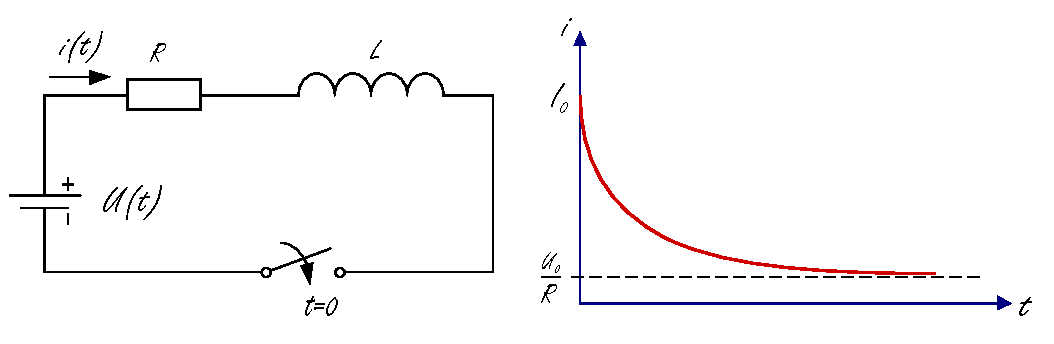
\includegraphics[width=\linewidth]{mai_fig032.pdf}
      \caption{Graf průběhu proudu $i(t)$ po sepnutí spínače v době $t=0$.}
      \label{mai:fig032}
    \end{figure}

%} %tikzset
%---------------------------------------------------------------------------------------------------
%\printbibliography[heading=subbibliography]
\addcontentsline{toc}{section}{Seznam literatury}
%  % !TeX spellcheck = cs_CZ
%{\tikzset{external/prefix={tikz/MAI/}}
% \tikzset{external/figure name/.add={ch11_}{}}
%---------------------------------------------------------------------------------------------------
% file NM.tex
%---------------------------------------------------------------------------------------------------
\chapter{Numerické metody}
\minitoc

  \section{Úvodní slovo}
    Numerické metody jsou metody, které na rozdíl od metod analytických poskytujících spojité řešení
    na určité předem definované oblasti, dávají čísel\-né řešení v předem zvolených diskrétních
    bodech této oblasti. Na rozdíl od analytických metod toto řešení většinou nebývá přesné, ale
    představuje pouze jeho aproximaci, která je zatížena určitou chybou.
    
    Možnosti analytických metod se již asi třicet let pokládají prakticky za vyčerpané. Drtivá
    většina problémů (a to zdaleka nejen v oblasti technických věd), které bylo možno analyticky
    vyřešit, již tehdy byla vyřešena. Při vyčíslování výsledků ovšem v mnoha případech nastávaly
    značné problémy; spojité řešení bylo například popsáno kombinací vyšších funkcí (Besselovy,
    Legendrovy atd.) v podobě nekonečných řad, přičemž bylo třeba načítat dostatečný počet jejich
    členů k dosažení požadované přesnosti. A zde se již začaly uplatňovat různé numerické techniky,
    které ovšem bylo v té době možno realizovat jen na kalkulačkách nebo ze současného pohledu na
    primitivních počítačích.
  
    Ačkoli základy sofistikovaných numerických metod byly položeny již před více než šedesáti lety,
    jejich intenzivní a široký rozvoj je spojen teprve s vývojem a zdokonalováním výpočetní techniky
    v posledních asi čtyřiceti letech a lze říci, že v poslední době s řešením čím dál tím
    složitějších problémů ze všech vědních oblastí (nestacionární a nelineární úlohy ve 2D a 3D)
    stále nabývají na významu.
  
    Výsledkem aplikace převážné většiny numerických metod je sestavení velkého systému lineárních či
    nelineárních algebraických rovnic, který je nutno nějakým způsobem vyřešit existují ovšem
    numerické techniky i pro jiné účely, jako je například součet různých řad, výpočet určitých
    integrálů atd., jejich počet však není příliš velký). A v popředí zájmu jsou především dvě
    otázky:
    \begin{itemize}
      \item jak sestavit onen systém tak, aby počet zmíněných rovnic byl co nej\-men\-ší (přičemž 
            ale informace o rozložení hledané veličiny v oblasti je maximální a co nejpřesnější) a
      \item jak tento systém vyřešit co nejrychleji a s nejmenší možnou chybou.
    \end{itemize}
    Na tomto místě je nutno podotknout, že i malá vylepšení stávajících postupů mohou při řešení
    složitých úloh vedoucích na řešení soustav milionů či desítek milionů rovnic (aktuální stav)
    zajistit velmi výrazné časové úspory. Samotná realizace jakékoli numerické metody sestává z
    několika kroků:
    \begin{itemize}
      \item Sestavení matematického modelu dané úlohy. Tento krok je sám o sobě často nesmírně
            komplikovaný; reálný fyzikální problém musíme mnohdy zjednodušit tak, aby byl vůbec
            dostupnými prostředky řešitel\-ný, aniž by však vzniklé chyby přesáhly přijatelné 
            hodnoty. Takový matematický model zpravidla sestává z různých rovnic (algebraických,
            diferenciálních, integrálních, smíšených), neurčitých nebo určitých integrálů a podobně.
      \item Výběr konkrétní metodiky, jakou tento model budeme řešit. Uvedená me\-to\-di\-ka by měla
            být co nejvýhodnější z celé řady hledisek, jako je rychlost výpočtu, spolehlivost,
            robustnost, přesnost, konvergence, stabilita atd. O těchto pojmech jistě už většinou 
            máme jakousi intuitivní představu, v dalším textu však některé z nich upřesníme. Na 
            základě zvolené metody vypracujeme algoritmus, což je konečné množství instrukcí, které 
            musíme provést, aby se celý výpočet bezezbytku provedl.
      \item Navržený algoritmus musíme nyní naprogramovat. Přitom lze využít buď nějakého
            programovacího jazyka (FORTRAN, C++ a další), nebo nějakého prostředí s již
            předprogramovanými operacemi nebo celými bloky výpočtů (MatLab, Mathematica). V 
            některých případech lze využít i již existujících profesionálních programů, které 
            takový algoritmus
            obsahují (freeware tohoto typu je velmi řídké). Ty jsou ovšem velmi drahé a uživatel do
            nich zpravidla nemůže zasahovat za účelem například optimalizace výpočtu.
      \item Dalším krokem je realizace výpočtu. Zde je kromě provedení samotného výpočtu nutné
            ověřit, že výsledky jsou korektní. K tomu používáme buď experiment, nebo jinou metodu,
            která je již pro úlohu daného typu spolehlivě prověřená. Dále ověřujeme celou řadu
            aspektů, jako je například geometrická konvergence řešení (závislost výsledků na hustotě
            diskretizační sítě) a popřípadě jiná kritéria, o nichž se více dozvíme později.
      \item Posledním krokem je vyhodnocení a posouzení získaných výsledků, zpravidla na vizuálním
            základě, porovnáním, ale i jinak.
    \end{itemize}
  
  \section{Reprezentace čísel ve výpočetní technice}
    Při realizaci numerických algoritmů na počítači se lze setkat se dvojí reprezentací čísel, a to
    pomocí \textbf{pevné} nebo \textbf{plovoucí desetinné tečky}. Pevná desetinná tečka znamená vždy
    předem definovaný počet desetinných míst. Pracujeme-li se čtyřmi desetinnými místy, interpretují
    se následující čísla takto:
  
    \begin{table}[h]
      \centering
        \begin{tabular}{l r}
          \hline
          8675             & 8675.0000  \\
          \quad  3.24      &    3.2400  \\
          \quad -0.000006  &   -0.0000  \\
          \hline
        \end{tabular}
        \caption{Reprezentace čísel v pevné desetinné tečce}
    \end{table}
  
    Zatímco první dvě čísla jsou zobrazena přesně, třetí číslo nikoli, je zaokrouhleno. Proto je
    tento způsob nepraktický, při vědeckotechnických výpočtech se neužívá a v dalším textu se jím už
    nebudeme zabývat.
  
    Daleko pružnější je proto počítání s plovoucí desetinnou tečkou, kdy se v každém čísle 
    respektuje předepsaný počet prvních číslic. V tomto případě se uvedená čísla zobrazují takto:
  
    \begin{table}[h]
      \centering
        \begin{tabular}{l c c l}
           \hline
           8675             & +0.8675E+04 & nebo & +8.675E+03  \\
           \quad  3.24      & +0.3240E+01 & nebo & +3.240E+00  \\
           \quad -0.000006  & -0.6000E-05 & nebo & -6.000E-06  \\
           \hline
        \end{tabular}
        \caption{Reprezentace čísel v plovoucí desetinné tečce}
    \end{table}
  
    Každé nenulové číslo a lze reprezentovat jako $a= +m\cdot10^e$ , kde $0.1 < m <1$ a $e$ je celé
    číslo. Samozřejmě, číslo $m$ může obsahovat nekonečnou řadu číslic a celé číslo $e$ se může
    pohybovat od minus nekonečna do nekonečna. To ale v počítačové reprezentaci není možné; zde je
    číslo $m$ omezeno na konečný počet $n$ číslic a právě tak je omezen i exponent. Číslo $a$ je 
    tedy počítačem aproximováno jako $a= \pm m\cdot10^e$, kde $m=0.d1d2\ldots dn$. Toto číslo $m$ se
    nazývá \textbf{mantisa} a $e$ \textbf{exponent}.
  
    V jednoduché přesnosti má v počítačích e velikost $|e|< 38$, ve dvojité přesnosti $|e|<308$.
    Jsou-li tyto hodnoty překročeny, vzniká chyba známá jako \textbf{underflow} nebo
    \textbf{overflow}.
  
    \subsection{Zaokrouhlování}
      Čísla jsou v počítačové interpretaci často zaokrouhlována (mají-li v mantise velký počet
      číslic), poněvadž mantisa $m$ zde může těchto číslic obsahovat pouze $n$. Pravidla
      zaokrouhlování jsou jasná. Zopakujeme zde jen to, že čísla typu 7.65 nebo 7.75 (chceme-li
      zrušit jedno desetinné místo) zaokrouhlíme tak, že poslední číslice je sudá. Takže zatímco 
      7.65 zaokrouhlíme na 7.6, 7.75 zaokrouhlíme na 7.8.
  
      Chybu při zaokrouhlování můžeme určit jako ($n$ je počet číslic v mantise $m$)
      \begin{equation}\label{nm:eq_err_round}
        |\frac{m-\underline{m}}{m}|\leq\frac{0.5}{10^{n-1}}
      \end{equation}  
  
  %============ Kapitola: Chyby při numerických výpočtech =========================================
  \section{Chyby při numerických výpočtech}
    Protože základem numerických metod je získávání přibližných výsledků, je nutné mít vždy
    představu, jaký rozdíl může být mezi přesným řešením dané úlohy a řešením získaným použitou
    numerickou metodou.
    \subsection{Zdroje a typy chyb}
      Pomineme-li jako zdroj chyb člověka dopouštějícího se omylů, můžeme chyby rozdělit na několik
      základních druhů.
      \begin{itemize}
        \item \textbf{Chyby matematického modelu} - vznikají nahrazením reálné fyzikální situace
              matematickým modelem. Může se jednat například o popis nějakého fyzikálního děje 
              pomocí diferenciální rovnice.
        \item \textbf{Chyby vstupních dat} - jsou způsobeny nepřesnostmi při měření fyzikálních
              veličin
        \item \textbf{Chyby numerické metody} - vznikají při náhradě původní matematické úlohy
              jednodušší numerickou. Často se jedná o náhradu nekonečného procesu procesem konečným,
              např. při výpočtu hodnoty některé elementární funkce pomocí součtu několika prvních
              členů její nekonečné Taylorovy řady nebo při aproximaci určitého integrálu souč\-tem
              konečného počtu funkčních hodnot. Odhad této chyby je důležitou součástí řešení každé
              numerické úlohy.
        \item \textbf{Chyby zaokrouhlovací} - vznikají tím, že při výpočtech pracujeme s čísly
              zaokrouhlenými na určitý, relativně nevelký počet míst. Tyto chyby se při výpočtu 
              mohou kumulovat, nebo navzájem rušit. Při vel\-kém počtu operací je posouzení jejich 
              vlivu velmi náročné.
      \end{itemize}
      
    \subsection{Definice chyb, šíření chyb při výpočtu}
      \subsection{Absolutní a relativní chyba}
        Je-li hodnota $\underline{c}$ aproximace přesné hodnoty $c$, je \textbf{absolutní chyba}
        definována jako $\varepsilon=c-\underline{c}$ a \textbf{relativní chyba}
        $\varepsilon_r=\frac{\varepsilon}{c},c\neq0$. Tato definice se může zdát neužitečná, 
        poněvadž $c$ neznáme. Lze-li však říci, že pokud se aproximace $\underline{c}$ blíží k $c$, 
        můžeme psát $\varepsilon_r=\frac{\varepsilon}{\underline{c}},\underline{c}\neq0$. Bohužel, 
        většinou neznáme ani hodnotu $\varepsilon$. Někdy však její hodnotu můžeme odhadnout vztahem
        $|\varepsilon|\leq\sigma$ a podobně lze odhadnout pro relativní chybu 
        $|\varepsilon_r|\leq\sigma_r$.
      \subsubsection{Šíření chyb}
        \emph{Meze absolutních chyb při sčítání a odečítání se rovnají součtu pří\-sluš\-ných mezí.
        Meze relativních chyb při násobení a dělení se rovnají součtu mezí jednotlivých relativních
        chyb}.
        \begin{itemize}
          \item Nechť  $|x_i-\hat{x}_i|=|\varepsilon_i|\leq\sigma_i,\quad i=1,\cdots,n$. Pak je
               \begin{equation}\label{nm:eq_sireni_abs_err}
                 |\sum_{i=1}^n{x_i-\hat{x}_i}|=|\sum_{i=1}^n{\varepsilon_i}|\leq\sum_{i=1}^n{\sigma_i}
               \end{equation}
  
          \item Nechť dále $|\frac{x_i-\hat{x}_i}{x_i}|=|\varepsilon_{ri}|\leq\sigma_{ri},\quad
                i=1,\cdots,n$. Pak je
  
               \begin{align*}
                 |\frac{\prod_{i=1}^n{x_i}-\prod_{i=1}^n{\hat{x}_i}}{\prod_{i=1}^n{x_i}}|      &=
                             |\frac{\prod_{i=1}^n{x_i}-\prod_{i=1}^n{x_i-\varepsilon_i}}
                             {\prod_{i=1}^n{x_i}}|\doteq
                             \\  
                 |\frac{\sum_{i=1}^n{\varepsilon_i}\prod_{j=1,j\neq i}^n{x_j}}
                             {\prod_{i=1}^n{x_i}}|                                             &=
                             |\sum_{i=1}^n{\frac{\varepsilon_i}{x_i}}|
                             \\
                 |\sum_{i=1}^n{\varepsilon_{ri}}|                                              &\leq
                             |\sum_{i=1}^n{\sigma_{ri}}|
              \end{align*}
        \end{itemize}
        kde jsme ale při rozdílu součinů v druhém výrazu zanedbali všechny násobky různých
        absolutních chyb, tedy členy druhého a vyšších řádů.
  
      \subsubsection{Podmíněnost numerických úloh a numerická stabilita algoritmů}
        Při numerickém řešení různých úloh musíme zkoumat, jaký vliv na výsledek mají malé změny ve
        vstupních hodnotách a zaokrouhlování během výpočtu. Řešení numerických úloh můžeme považovat
        za postup, kterým přiřazujeme vstupním údajům výstupní data. Je-li toto přiřazení spojité
        zobrazení, pak říkáme, že numerická úloha je \textbf{korektní úloha}, v opačném případě se
        jedná o úlohu \textbf{nekorektní}.
  
        Pro tyto úlohy má zásadní význam relativní citlivost výsledku na malé změny ve vstupních
        parametrech úlohy. Korektní úloha je \textbf{dobře pod\-mí\-ně\-ná}, jestliže malým
        relativním změnám vstupních údajů odpovídají malé relativní změny výstupních údajů. Číslo
        \begin{equation}\label{nm:eq_podminenost}
          C_p=\frac{\texttt{relativní chyba výstupnich údajů}}{\texttt{relativní chyba vstupních
              údajů}},
        \end{equation}
        nazýváme \textbf{číslo podmíněnosti úlohy}. Pro dobře podmíněné úlohy je číslo $C_p$ blízké
        číslu $1$. Pokud malé relativní změny na vstupu způsobí velké relativní změny na výstupu, 
        pak  mluvíme o \emph{špatně podmíněné úloze}. Řešení špatně podmíněných úloh je nejlépe se
        vyhnout, protože výsledky jakéhokoliv algoritmu jsou velmi nespolehlivé. Podobně řekneme, že
        je algoritmus \emph{dobře pod\-mí\-ně\-ný}, je-li málo citlivý na poruchy ve vstupních
        datech. Kromě ne\-přes\-ností ve vstupních údajích ovlivňuje výsledek použitého algoritmu i
        zaokrouhlování čísel během výpočtu. Je-li vliv zaokrouhlovacích chyb na výsledek malý,
        mluvíme o \emph{numericky stabilním algoritmu}. \emph{Algoritmus dobře pod\-mí\-ně\-ný a
        numericky stabilní se nazývá stabilní}.
  
  %=============== Kapitola: Řešení nelineárních rovnic ============================================
  \section{Řešení nelineárních rovnic}
    \subsection{Motivace}
      Kořeny nelineárních rovnice $f(x)=0$ obecně neumíme vyjádřit explicitním vzorcem. K řešení
      nelineární rovnice proto používáme iterační metody: z jedné nebo několika počátečních
      aproximací hledaného kořene $\hat{x}$ generujeme posloupnost $x_0,x_1,x_2…$, která ke kořenu
      $\hat{x}$ konverguje. Pro některé metody stačí, když zadáme interval $\langle a,b\rangle$,
      který obsahuje hledaný kořen. Jiné metody vyžaduji, aby počáteční aproximace byla k hledanému
      kořenu dosti blízko; na oplatku takové metody konvergují mnohem rychleji. Často proto začínáme
      s \uv{hrubou}, avšak spolehlivou metodou, a teprve když jsme dostatečně blízko kořene, 
      přejdeme na \uv{jemnější}, rychleji konvergující metodu.
  
      Abychom naše úvahy zjednodušili, omezíme se na problém určení re\-ál\-né\-ho
      je\-dno\-du\-ché\-ho kořene $\hat{x}$ rovnice $f(x)=0$, tj. předpokládáme, že $f'(\hat{x})=0$.
      Budeme také automaticky předpokládat, z funkce $f(x)$ je spojitá a má tolik spojitých 
      derivací, kolik je jich v dané situaci zapotřebí.
  
      Počáteční aproximaci kořenů rovnice $f(x)=0$ můžeme zjistit z grafu funkce $f(x)$: ručně, nebo
      raději pomocí vhodného programu na počítači, vykreslíme funkci $f(x)$ a vyhledáme její
      průsečíky s osou $x$.
  
      Jinou možností je sestaveni tabulky $[x_i,f(x_i)]$ pro nějaké dělení:
      $$a=x_0<x_1<\cdots<x_{i-1}<x_i<\cdots<x_n=b$$.
      \begin{example} Získejme hrubý odhad kořenů rovnice $f(x) = 0$, kde $$f(x):y=4\sin x - x^3 - 
      1$$

          {\centering
           \captionsetup{type=figure}
           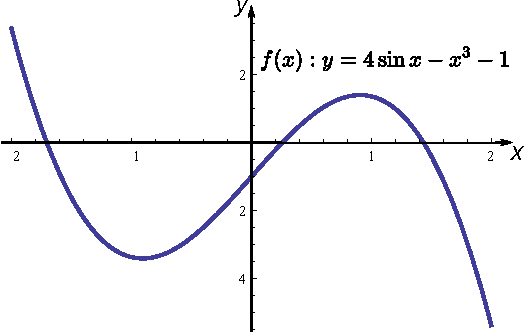
\includegraphics[scale=1]{mai_fig035.pdf}
           \captionof{figure}{Graf funkce $f(x):y=4\sin x - x^3 - 1$.}
           \label{mai:fig035}
           \par}
        Z obrázku \ref{mai:fig035} zjistíme, že existují tři kořeny: $x_1^*\in(-2,-1),
        x_2^*\in(-1, 0)$ a $x_3^*\in(1, 2)$.
      \end{example}
  
      Z obrázku zjistíme, že existují tři kořeny: $x_1^*\in(-2,-1),x_2^*\in(0,1),x_3^*\in(1,2)$.
      Zkusme najít kořeny v těchto intervalech pomocí numerických metod popsaných v následujících
      odstavcích
  
    \subsection{Metoda bisekce}
      Metoda známá také jako \textbf{metoda půlení intervalů}, je založena na principu
      zna\-mén\-ko\-vých změn. Předpokládejme, že funkce $f(x)$ má v koncových bodech intervalu
      $(a_0,b_0)$ opačná znaménka, tj. platí $f(a_0 )\cdot f(b_0 )<0$. Sestrojíme posloupnost
      intervalů $(a_1,b_1)\supset(a_2,b_2)\supset(a_3,b_3)\supset\cdots$, které obsahují kořen.
      Intervaly $(a_{k+1},b_{k+1}), k=0,1,\cdots$, určíme rekurzivně způsobem, který si nyní
      popíšeme.
  
      Střed intervalu $(a_k,b_k)$ je bod $x_{k+1}=\frac{1}{2}(a_k+b_k)$. Když $f(x_k)=0$, pak
      $x_{k+1}=x^*$ je kořen a dál nepokračujeme.

%} %tikzset
%---------------------------------------------------------------------------------------------------
\printbibliography[heading=subbibliography]
\addcontentsline{toc}{section}{Seznam literatury}
%  % !TeX spellcheck = cs_CZ
%     An overview of high school mathematics
%{\tikzset{external/prefix={tikz/MAI/}}
% \tikzset{external/figure name/.add={ch01_}{}}
%---------------------------------------------------------------------------------------------------
% history_MA.tex
%---------------------------------------------------------------------------------------------------
\setchaptertoc
\chapter{Historie matematické analýzy} %\label{mai:IchapI}

  Analýza jako nezávislý předmět byla vytvořena v 17. stol. během vědecké revoluce. Kepler, 
  Galilei, Descartes, Fermat, Huygens, Newton a Leibniz, když zmíníme jen několik důležitých jmen 
  těch, kteří přispěli k jejímu vzniku. Otázky z mechaniky, optiky a astronomie hráli roli v jejím 
  raném období, tak jako vnitřní problémy matematiky, jako výpočet obsahů, objemů a analýza 
  komplikovaných křivek. Pohyb po zakřivených drahách působením proměnných sil, které se staly 
  předmětem důkladného zájmu po studiu volně padajících těles Galilea, vedl k počátečnímu úspěchu. 
  Z velké rozmanitosti snah, které se objevily na konci 17. stol. v práci Newtona a Leibnize, se 
  zrodila nová matematická disciplína, jejíž některé poznatky jsou v těchto studijních zápiscích.
  
  Základní myšlenka použití diferenciálních rovnic k získání pohledu na globální chování proměnných
  kvantit z jejich (infinitezimálních) změn prokázala základní a plodné výsledky daleko za hranicemi
  matematiky a fyzika a formovala náš souhrnný vědecký pohled na svět, zvláště na představu o
  kauzalitě. Na konci 18. stol., vskutku, největší vědci došli ke shodě, že procesy v přírodě (a
  společnosti) jsou determinovány a podřízeny zákonům, které mohou být popsány v podobě
  diferenciálních rovnic. Laplace, tento mistr matematické fyziky, naznačil obraz nějaké fiktivní
  vševědoucí inteligence, užívající úplnou znalost zákonů a stavu světa v daný časový okamžik, by
  mohla předpovídat další vývoj světa navždy a hned. Myšlenka \emph{přírodních zákonů} byla kmotrem
  při vytvoření matematického pojmu funkce a naopak nebyla by to myšlenka nikdy tak vlivná, kdyby
  matematická analýza nevyvíjela úspěšné metody pro výzkum funkčních závislostí. 

%} % tikzset
%---------------------------------------------------------------------------------------------------              
}
{
% DEBUG was off
%-------------------Introduction to mathematical analysis -----------------------------------------
  % !TeX spellcheck = cs_CZ
%     An overview of high school mathematics
%{\tikzset{external/prefix={tikz/MAI/}}
% \tikzset{external/figure name/.add={ch01_}{}}
%---------------------------------------------------------------------------------------------------
% history_MA.tex
%---------------------------------------------------------------------------------------------------
\setchaptertoc
\chapter{Historie matematické analýzy} %\label{mai:IchapI}

  Analýza jako nezávislý předmět byla vytvořena v 17. stol. během vědecké revoluce. Kepler, 
  Galilei, Descartes, Fermat, Huygens, Newton a Leibniz, když zmíníme jen několik důležitých jmen 
  těch, kteří přispěli k jejímu vzniku. Otázky z mechaniky, optiky a astronomie hráli roli v jejím 
  raném období, tak jako vnitřní problémy matematiky, jako výpočet obsahů, objemů a analýza 
  komplikovaných křivek. Pohyb po zakřivených drahách působením proměnných sil, které se staly 
  předmětem důkladného zájmu po studiu volně padajících těles Galilea, vedl k počátečnímu úspěchu. 
  Z velké rozmanitosti snah, které se objevily na konci 17. stol. v práci Newtona a Leibnize, se 
  zrodila nová matematická disciplína, jejíž některé poznatky jsou v těchto studijních zápiscích.
  
  Základní myšlenka použití diferenciálních rovnic k získání pohledu na globální chování proměnných
  kvantit z jejich (infinitezimálních) změn prokázala základní a plodné výsledky daleko za hranicemi
  matematiky a fyzika a formovala náš souhrnný vědecký pohled na svět, zvláště na představu o
  kauzalitě. Na konci 18. stol., vskutku, největší vědci došli ke shodě, že procesy v přírodě (a
  společnosti) jsou determinovány a podřízeny zákonům, které mohou být popsány v podobě
  diferenciálních rovnic. Laplace, tento mistr matematické fyziky, naznačil obraz nějaké fiktivní
  vševědoucí inteligence, užívající úplnou znalost zákonů a stavu světa v daný časový okamžik, by
  mohla předpovídat další vývoj světa navždy a hned. Myšlenka \emph{přírodních zákonů} byla kmotrem
  při vytvoření matematického pojmu funkce a naopak nebyla by to myšlenka nikdy tak vlivná, kdyby
  matematická analýza nevyvíjela úspěšné metody pro výzkum funkčních závislostí. 

%} % tikzset
%---------------------------------------------------------------------------------------------------              
%---------------------Reálná a komplexní čísla-----------------------------------------------------
  % !TeX spellcheck = cs_CZ
% Basis of Linear Algebra:
%{\tikzset{external/prefix={tikz/MAI/}}
% \tikzset{external/figure name/.add={ch02_}{}}
%---------------------------------------------------------------------------------------------------
% intro_linear_algebra.tex
%---------------------------------------------------------------------------------------------------
% ==================================================================================================
% In linear algebra, a basis is a set of linearly independent vectors that, in a
% linear combination, can represent every vector in a given vector space or free
% module, or, more simply put, which define a "coordinate system".[1] In more
% general terms, a basis is a linearly independent spanning set. 
% --------------------------------------------------------------------------------------------------
\chapter{Všemocná úměra aneb lineární algebra poprvé}\label{mai:IchapII}
\minitoc
  Tuto kapitolu bychom mohli opatřit podtitulem \emph{„To nejnutnější z lineární algebry“}. 
  Dovíme se v ní, co je třeba si představit pod pojmem \emph{„linearita“}, najdeme příklady 
  linearity v geometrii i v přírodovědě (fyzice, chemii, biologii) a formulujeme základní 
  poznatky týkající se řešení soustav lineárních rovnic. Do této oblasti patří i počítání s 
  vektory a maticemi - objekty, které jsou velmi vhodné k vyjádření fyzikálních veličin.
    
  \section{Lineární rovnice}\label{mai:IchapIIsecI}
    Co tedy znamená slovo \textbf{linearita}? Pochází z latiny, \emph{linea recta = přímka}, 
    česky bychom řekli \emph{přímá úměrnost} nebo jen jednoduše \emph{úměra}.
    
    Nejjednodušší příklady linearity patří do oblasti geometrie - vyjádření \emph{přímek} a 
    \emph{rovin}. Jistě si ze střední školy vzpomínáme, že body těchto útvarů popisujeme jejich 
    souřadnicemi na přímce \(\mathbb{R}\), v rovině \(\mathbb{R}^2\), v prostoru \(\mathbb{R}^3\). 
    Souřadnice bodu v rovině tedy tvoří \emph{uspořádanou dvojici} reálných čísel, v prostoru pak 
    \emph{uspořádanou trojici} reálných čísel. (Pozor, dvojice \([a, b]\) a \([b, a]\) představují 
    různé body.)

    %--Parametrické vyjádření přímky--------------------------------
        % !TeX spellcheck = cs_CZ
% Musilova2009MA1
\wikitextrule
\begin{example}\label{mai:exam001}
  \textbf{Parametrické vyjádření přímky}\newline\small
  \emph{Přímka} — jednorozměrný lineární útvar v jednorozměrném prostoru \(\mathbb{R}^1\), 
  dvojrozměrném prostoru \(\mathbb{R}^2\), trojrozměrném prostoru \(\mathbb{R}^3\) (nebo i 
  n-rozměrném prostoru \(\mathbb{R}^n\)), je určena dvěma body, třeba \(A\) a \(B\), nebo 
  ekvivalentně, bodem \(A\) a \emph{směrovým} vektorem \(\vec{u}\) (obr. \ref{mai:fig000}). 
  Je-li \(X\) obecným bodem na této přímce, je vektor \(\overrightarrow{AX}\) rovnoběžný, 
  tj. \emph{kolineární}, se směrovým vektorem \(\vec{u}\). (Jako směrový můžeme samozřejmě 
  použít i vektor \(\overrightarrow{AB}\).) Vektor \(\overrightarrow{AX}\) má tedy s 
  vektorem \(\vec{u}\) stejný směr, lišit se může velikostí nebo orientací. Tuto skutečnost 
  zapíšeme tak, že \(\overrightarrow{AX}\) je \(t\)-násobkem vektorů \(\vec{u}\),
  \begin{equation*}
  \overrightarrow{AX} = t \cdot \vec{u}.
  \end{equation*}
  {\centering
    \captionsetup{type=figure}
    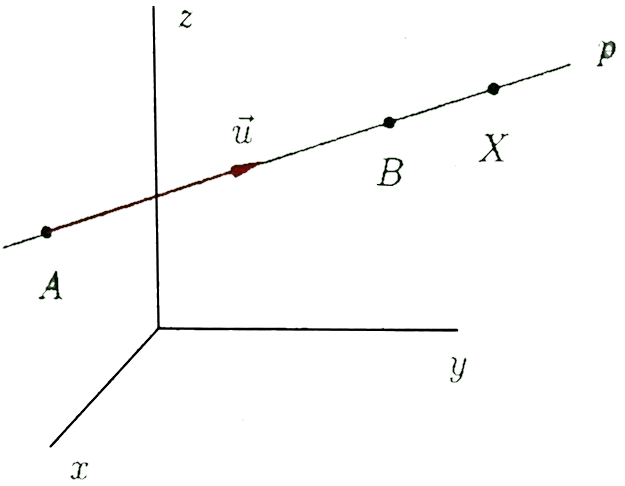
\includegraphics[width=0.4\linewidth]{mai_fig000.png}
    \captionof{figure}{Zadáni přímky. \cite[s.~1]{Musilova2009MA1}
    \label{mai:fig000}}
    \par}
  Veličinou \(t\), takzvaným \emph{parametrem}, který může nabývat všech reálných hodnot, 
  \(t\in\mathbb{R}\), dokážeme popsat všechny vektory \(\overrightarrow{AX}\), jejichž 
  koncový bod \(X\) leží na přímce \(p\). Naopak, žádné jiné body \(X\) než ty, které leží na 
  přímce \(p\), tuto vlastnost nemají. S označením bodů \(A\), \(X\), resp. vektorů 
  \(\vec{u}\), \(\overrightarrow{AX}\) kartézskými souřadnicemi, resp. složkami
  \begin{align*}
                    A &= (x_A,y_A, z_A), \\ 
                    X &=(x,y,z),         \\
              \vec{u} &= (u_1,u_2,u_3),  \\ 
  \overrightarrow{AX} &= (x - x_A, y - y_1A, z-z_A),
  \end{align*}
  dostáváme \textbf{parametrické vyjádřeni přímky} \(p\) ve tvaru
  \begin{equation}\label{MAI:eq_M001}
    p = \left\{(x,y,z)\in\mathbb{R}^3\,|\,
    \begin{matrix}
      x = x_A + tu_1,        \\
      y = y_A + tu_2,        \\
     z = z_A + tu_3,
    \end{matrix}
    \;t\in\mathbb{R}
    \right\}. 
  \end{equation}
  \normalsize
\end{example}
    %---------------------------------------------------------------
    
    Vidíme, že kartézské souřadnice bodu na přímce se vůči souřadnicím bodu \(A\) mění přímo 
    úměrně v závislosti na hodnotě parametru \(t\), tj. závisí na jeho první mocnině. Příslušná 
    závislost se nazývá \textbf{lineární funkcí}.
    
    Obdobně zapíšeme parametrické vyjádření roviny v \(\mathbb{R}^3\):
    
    %--Parametrická vyjádření roviny--------------------------------
    % !TeX spellcheck = cs_CZ
\begin{mathexam}{Parametrická vyjádření roviny}{exam004}
  Rovina v trojrozměrném prostoru \(\mathbb{R}^3\) je zadána třemi body \(A\), \(B\) a \(C\), které
  nesmějí ležet v jedné přímce, popřípadě dvěma body \(A\) a \(B\) a vektorem \(\vec{v}\)
  nerovnoběžným s \(\overrightarrow{AB}\), anebo bodem \(A\) a dvěma nerovnoběžnými směrovými
  vektory \(\vec{u}\) a \(\vec{v}\) (obr. \ref{mai:FIG002}). Všechny tyto typy zadání jsou
  ekvivalentní. Lze volit například \(\vec{u} = \overrightarrow{AB}\), \(\vec{v} =
  \overrightarrow{AC}\). Je-li \(X\) libovolným bodem roviny \(\varrho\), jsou vektory
  \(\overrightarrow{AX}\), \(\vec{u}\) a \(\vec{v}\) \textbf{lineárně závislé}. To znamená, že
  existují taková reálná čísla \(r\) a \(s\), že vektor \(\overrightarrow{AX}\) lze zapsat jako
  lineární kombinaci

  \begin{equation*}
    \overrightarrow{AX} = r\cdot\vec{u} + s\cdot\vec{v}, \qquad r,s \in\mathbb{R}
  \end{equation*}
  Při obdobném zápisu kartézských souřadnic bodů a složek vektorů jako u vyjádření přímky dostaneme
  parametrické vyjádření roviny \(\varrho\)
  \begin{equation*}
    \varrho = \left\{
    \begin{matrix}  
      (x,y,z)\in\mathbb{R}^3  \\
      r, s \in\mathbb{R}
    \end{matrix}
    \,\left\lvert\,
    \begin{matrix}
      x = x_A + ru_1 + sv_1,        \\
      y = y_A + ru_2 + sv_2,        \\
      z = z_A + ru_3 + sv_3,
    \end{matrix}\right.          
    \right\}.
  \end{equation*} 

  { \centering
    \captionsetup{type=figure}
    \luafigure[1]{mai_fig026.pdf}
    \captionof{figure}{Zadání roviny. \cite[s.~3]{Musilova2009MA1}
    \label{mai:FIG002}} \par}

  Toto vyjádření obsahuje opět lineární závislost: Souřadnice \(x\), \(y\) a \(z\) se vůči
  souřadnicím bodu \(A\) mění v závislosti na prvních mocninách parametrů \(r\) a \(s\). Můžeme tak
  hovořit o jakési „vícerozměrné úměře“.
\end{mathexam}
  
    %---------------------------------------------------------------
    
    Všimněme si nyní příkladů linearity z oblasti přírodovědy.
    
    %--Fyzika — Ohmův zákon-----------------------------------------
    % !TeX spellcheck = cs_CZ
% \wikitextrule
\begin{mdframed}[style=mdexam]
  \begin{example}\label{mai:exam035}
    \textbf{Fyzika - Ohmův zákon:}\newline
    Z elektřiny víme, že některé vodiče či elektrické prvky se při průchodu elektrického proudu 
    chovají podle zákona linearity: Proud, který jimi protéká, závisí přímo úměrně na přiloženém 
    napětí (obr. \ref{mai:fig036}). Platí \(I(U) = R^{-1 }U\) s konstantou úměrnosti \(R^{-1}\), kde 
    \(R\) je elektrický odpor vodiče (prvku).

    Pozn. 1: Předpokládáme, že elektrický odpor voltmetru je tak velký, že proud jím procházející je 
    z hlediska přesnosti měření zanedbatelný.
    
    Pozn. 2: Graf závislosti proudu na napětí na obrázku \ref{mai:fig036} může pro vyšší hodnoty 
    napětí vykazovat odchylku od linearity (přímkové závislosti), neboť se prvek při vyšším proudu 
    zahřívá a jeho odpor roste.
    
    {\centering
      \captionsetup{type=figure}
      \luafigure[1]{mai_fig036.png}
      \captionof{figure}{Chování lineárního vodiče (Ohmův zákon). \cite[s.~15]{Musilova2009MA1}
      \label{mai:fig036}}
      \par}  
  \end{example}
\end{mdframed}
    %---------------------------------------------------------------

    %--Fyzika — speciální typy pohybů-------------------------------
    % !TeX spellcheck = cs_CZ
\wikitextrule
\begin{example}\label{mai:exam036}
  \textbf{Fyzika — speciální typy pohybů:}\newline\small
  Při rovnoměrném pohybu tělesa (ať již přímočarém či křivočarém) je dráha, kterou těleso urazí za 
  dobu \(t\), přímo úměrná velikosti jeho rychlosti \(v\), tj. \(s(t) = s_0 + vt\). Při pohybu 
  rovnoměrně zrychleném (zpožděném) je lineární závislost velikosti rychlosti na čase, tj. \(v(t) = 
  v_0 \pm at\) při pohybu přímočarém (\(a\) je velikost zrychlení), nebo \(v(t) = v_0 \pm a_\tau 
  t\) při pohybu křivočarém (\(a_\tau\) je velikost průmětu zrychlení do směru tečny k 
  trajektorii tělesa — tečného zrychlení).
  \normalsize
\end{example}
    %---------------------------------------------------------------
    
  \subsection{Soustavy lineárních rovnic a jejich rychlé řešení}
    Příkladů linearity v přírodě bychom mohli nalézt bezpočet. Vraťme se však k matematice a k 
    problematice uvedené v názvu tohoto odstavce, k soustavám lineárních rovnic. Začněme 
    jednoduchou slovní úlohou ze základní školy:
    
    %--Jeníček a Mařenka kradli ježibabě perník---------------------
    % !TeX spellcheck = cs_CZ
% \wikitextrule
\begin{mdframed}[style=mdexam]
  \begin{example}\label{mai:exam037}
    \textbf{Jeníček a Mařenka kradli ježibabě perník:}\newline
    Dohromady snědli \num{11} perníkových srdíček. Jeníček jich přitom zkonzumoval o \num{3} více
    než Mařenka. Otázka je tradiční - kolik srdíček snědl každý z nich? Označíme-li \(M\) počet
    kousků, které snědla Mařenka a \(J\) počet srdíček, na nichž si pochutnal Jenda, můžeme
    informace zadané v úloze zapsat takto:
    \begin{equation*}
      M + J = 11, \qquad J = M + 3.
    \end{equation*}
    
    Řešení není problémem, snadno vidíme, že \(M = 4\) a \(J = 7\).
  \end{example}
\end{mdframed}
    %---------------------------------------------------------------
    
    O samotné řešení této jednoduché úlohy v tuto chvíli nejde. Pojmenujme si však vztahy, které 
    jsme pro neznámé hodnoty \(M\) a \(J\) ze zadání úlohy dostali. Neznámé vystupují v 
    rovnicích v první mocnině, tedy \emph{lineárně}. Máme \emph{soustavu dvou rovnic} o dvou 
    neznámých \(M\) a \(J\). Úvahu snadno zobecníme: Předpokládejme, že máme neznámé veličiny
    \begin{equation*}
      (x_1, x_2, \ldots, x_n)
    \end{equation*}
    a máme o nich \(m\) informací, které lze zapsat ve tvaru lineárních rovnic (neznámé budou v 
    těchto rovnicích vystupovat v první mocnině),
    \begin{align}
      a_{11}x_1 + a_{12}x_2 + \ldots + a_{1n}x_n &= b_1,     \nonumber           \\
      a_{21}x_1 + a_{22}x_2 + \ldots + a_{2n}x_n &= b_2,     \label{mai:eq002}   \\
      .......................................... &= \ldots   \nonumber           \\
      a_{m1}x_1 + a_{m2}x_2 + \ldots + a_{mn}x_n &= b_m,     \nonumber
    \end{align}
    Soustavu (\ref{mai:eq002}) nazýváme soustavou \(m\) lineárních rovnic o \(n\) neznámých. 
    Označme ji jako \(S\) a pod tímto označením se k ní budeme vracet. Soubory reálných čísel 
    \((a_{ij})\) a \((b_i)\), kde \(1 < i < m\), \(1 \leq j < n\), jsou zadány. Lze je uspořádat 
    do takzvaných \textbf{matic}:
    \begin{equation}\label{mai:eq003}
      \matr{A} =
        \begin{pmatrix}
          a_{11} & a_{12} & \ldots & a_{1n} \\
          a_{21} & a_{22} & \ldots & a_{2n} \\
          \ldots & \ldots & \ldots & \ldots \\
          a_{m1} & a_{m2} & \ldots & a_{mn}          
        \end{pmatrix},
        \overline{\matr{B}} =
        \begin{pmatrix}
          b_1     \\
          b_2     \\
          \ldots  \\
          b_m 
        \end{pmatrix}
    \end{equation}
    
    Matice \(\matr{A}\) je typu \(m/n\), má \(m\) řádků a \(n\) sloupců, \(i\) je řádkový index a 
    \(j\) je sloupcový index. Matice \(\overline{\matr{B}}\) je typu \(m/1\) (\(m\) řádků a jeden 
    sloupec), hovoříme také o sloupcové matici. Soustavu \(S\) můžeme zapsat zkráceně pomocí 
    maticového násobení (podrobněji viz později odstavec \ref{mai:IchapIIsecIII}):
    \begin{equation*}
      \matr{A} \cdot \matr{X} = \matr{B}, \qquad \text{nebo}
    \end{equation*}  
    \begin{equation}\label{mai:eq004}
        \begin{pmatrix}
          a_{11} & a_{12} & \ldots & a_{1n} \\
          a_{21} & a_{22} & \ldots & a_{2n} \\
          \ldots & \ldots & \ldots & \ldots \\
          a_{m1} & a_{m2} & \ldots & a_{mn}
        \end{pmatrix}
        \cdot
        \begin{pmatrix}
          x_1     \\
          x_2     \\
          \ldots  \\
          x_m 
       \end{pmatrix}
        =
       \begin{pmatrix}
            b_1     \\
            b_2     \\
            \ldots  \\
            b_m 
          \end{pmatrix}
    \end{equation}
    V tuto chvíli vysvětlíme podstatu maticového násobení jen technicky: Násobit mezi sebou  můžeme matici 
    \(\matr{A} = (a_{ij})\) typu \(m/n\) (levý činitel) a matici \(\matr{A} = (c_{jk})\) typu 
    \(n/p\) (pravý činitel, činitele nelze zaměňovat). Výsledkem je matice \(\matr{A} = (d_{ik})\) 
    typu \(m/p\), jejíž prvky se počítají podle předpisu
    \begin{equation}\label{mai:eq005}
      d_{ik} = \sum_{j=1}^{n} a_{ij}\cdot c_{jk}.
    \end{equation}
    
    Z tohoto obecného předpisu vidíme, že levé strany soustavy \(S\) lze interpretovat ve tvaru 
    součinu matice \(A\) typu \(m/n\) s maticí neznámých typu \((n/1)\), výsledkem je matice 
    pravých stran \(\overline{\matr{B}}\), která je typu \(m/1\). Matice \(\matr{A}\) se nazývá 
    \textbf{maticí soustavy}. Matice, která vznikne jejím \emph{rozšířením} o sloupec pravých 
    stran, tj.
    \begin{equation}\label{mai:eq006}
      \matr{B} = (\matr{A}|\overline{\matr{B}}) =
      \left(
        \begin{array}{cccc|c}
          a_{11} & a_{12} & \ldots & a_{1n} & b_1    \\
          a_{21} & a_{22} & \ldots & a_{2n} & b_2    \\
          \ldots & \ldots & \ldots & \ldots & \ldots \\
          a_{m1} & a_{m2} & \ldots & a_{mn} & b_m
        \end{array}
      \right)
    \end{equation}
    je pak \textbf{rozšířenou maticí soustavy}. Je-li sloupec pravých stran soustavy tvořen 
    samými nulami, nazývá se soustava \textbf{homogenní}, v opačném případě \textbf{nehomogenní}. 
    Řešením soustavy \(S\) nazýváme každou \(n\)-tici \((x_i, x_2,\ldots, x_n)\), která soustavu 
    \(S\) splňuje. Cílem je najít všechna řešení soustavy \(S\). Abychom řešení nalezli, musíme 
    soustavu upravovat, zjednodušovat. Prováděné úpravy mají vést k jednodušší, avšak 
    ekvivalentní soustavě rovnic, tj. takové, která má naprosto stejný soubor všech řešení jako 
    soustava původní. Takové úpravy nazýváme \textbf{ekvivalentními}. Dvě základní, pomocí nichž 
    lze uskutečnit všechny ostatní, jsou
    \begin{itemize}\addtolength{\itemsep}{-0.5\baselineskip}
      \item vynásobení libovolné, například \(i\)-té, rovnice libovolným \emph{nenulovým} číslem,
      \item přičtení \(i\)-té rovnice vynásobené libovolným číslem k \(l\)-té rovnici.
    \end{itemize} 
    V soustavě lze samozřejmě také měnit pořadí rovnic. Tato úprava je rovněž ekvivalentní. 
    Nevypisujeme ji však zvlášť proto, že ji lze realizovat pomocí vhodně zvolené posloupnosti 
    základních dvou úprav.
    
    Abychom nemuseli soustavu stále opisovat i s neznámými, provádíme obvykle ekvivalentní 
    úpravy jen s maticí \(\matr{B} = (\matr{A}|\overline{\matr{B}})\) (každý řádek této matice 
    představuje jednu rovnici soustavy \(S\)). Může se stát, že soustava má právě \emph{jedno 
    řešení}, jako tomu bylo v  úloze o Mařence a Jeníčkovi. Také nemusí mít \emph{řešení žádné}, 
    jako například soustava \(x + y = 0\), \(x + y = 1\) (součet dvou čísel nemůže nabývat současně 
    dvou různých hodnot). A třeba má také řešení \emph{nekonečně mnoho} (řešením soustavy jedné 
    rovnice o dvou neznámých \(x + y = 1\) jsou všechny dvojice tvaru \((x, 1 - x)\), kde \(x\) je 
    libovolné). A může mít soustava \(S\) třeba právě dvě řešení? Prostřednictvím následujícího 
    příkladu ukážeme metodu, která vede velmi rychle k nalezení všech řešení a umožňuje také 
    vyslovit obecné závěry o jejich vlastnostech a počtu. Jedná se o \textbf{Gaussovu eliminační 
    metodu}.

    %Gaussova eliminační metoda-------------------------------------
    \begin{mathexam}{Gaussova eliminační metoda}{exam038}
  Je zadána soustava tří (\(m = 3\)) rovnic o pěti (\(n = 5\)) neznámých:
  \begin{alignat*}{7}
       x_1 &+ 2x_2 &-  x_3 &+  x_4 &- 5x_5 &=  &&0, \\
     -2x_1 &- 4x_2 &+ 2x_3 &+ 4x_4 &+ 4x_5 &= -&&6, \\
      -x_1 &- 2x_2 &+  x_3 &+ 5x_4 &-  x_5 &=  &&6.
  \end{alignat*}
  Budeme provádět ekvivalentní úpravy matice \(\matr{B}\) tak, abychom ji zjednodušovali.
  Ekvivalenci matic budeme označovat znakem \(\sim\). 
  \begingroup
    \renewcommand\arraystretch{1.0}
    \renewcommand\arraycolsep{3pt}
    \begin{equation*}
      \matr{B} = (\matr{A}\lvert\overline{\matr{B}}) =
      \left(
        \begin{array}{rrrrr|r}
           1 &  2 & -1 & 1 & -5 &  0    \\
          -2 & -4 &  2 & 4 &  4 & -6    \\
          -1 & -2 &  1 & 5 & -1 &  6
        \end{array}
      \right).
    \end{equation*}
  \endgroup
  V prvním řádku je na první pozici jednička. Toho využijeme k snadné „likvidaci“, tedy eliminaci,
  prvních prvků v druhém a třetím řádku pomocí elementárních úprav. Provedeme tyto dvě úpravy:
  první řádek vynásobený číslem \num{2} přičteme k druhému řádku, první řádek přičteme ke třetímu
  řádku. Dostaneme
  \begingroup
    \renewcommand\arraystretch{1.0}
    \renewcommand\arraycolsep{3pt}
    \begin{equation*}
      \matr{B} \sim
      \left(
        \begin{array}{rrrrr|r}
          1 &  2 & -1 & 1 & -5 &  0         \\
          \bm{0} &  0 &  0 & 6 & -6 & -6    \\
          \bm{0} &  0 &  0 & 6 & -6 &  6
        \end{array}
      \right).
    \end{equation*}
  \endgroup  
  Vidíme, že jsme v druhém i třetím řádku dostali na první sloupcové pozici nulu (tučná). (Nuly na
  dalších  pozicích vznikly náhodou, vlivem jednoduchosti zadání.) Nyní vynásobíme druhý i třetí
  řádek číslem (\num{1/6}):
  \begingroup
    \renewcommand\arraystretch{1.0}
    \renewcommand\arraycolsep{3pt}    
    \begin{equation*}
      \matr{B} \sim
      \left(
        \begin{array}{rrrrr|r}
                1 &  2 & -1 & 1 & -5 &  0    \\
                0 &  0 &  0 & 1 & -1 & -1    \\
                0 &  0 &  0 & 1 & -1 &  1
        \end{array}
      \right).
    \end{equation*}
  \endgroup  
  Přestože již nyní vidíme, že soustava nemá řešení (rovnice druhého a třetího řádku znějí \(x_4 -
  x_5 = - 1\) a \(x_4 -x_5 = 1\), takže jim nevyhovuje žádná dvojice čísel \((x_4, x_5)\)), budeme
  v eliminaci pokračovat. Další úpravy se již týkají pouze druhého a třetího řádku. Druhý řádek
  vynásobený (\num{-1}) přičteme ke třetímu. Pak

  \begingroup
  \renewcommand\arraystretch{1.0}
  \renewcommand\arraycolsep{3pt}
    \begin{equation*}
      \matr{B} \sim
      \left(
        \begin{array}{rrrrr|r}
                1 &  2 & -1 & 1      & -5 &  0    \\
                0 &  0 &  0 & 1      & -1 & -1    \\
                0 &  0 &  0 & \bm{0} &  0 &  2
        \end{array}
      \right).
    \end{equation*}
  \endgroup  
  Získáváme tak ekvivalentní soustavu rovnic
  \begin{alignat*}{5}
        x_1 + 2x_2 - x_3 &+  x_4 &- 5x_5 &=  &&0, \\
                         &+  x_4 &-  x_5 &= -&&1, \\
                         &       &     0 &=  &&2.
  \end{alignat*}
  V poslední rovnici je ihned vidět rozpor - soustava nemá řešení
\end{mathexam}
    %---------------------------------------------------------------

    Na základě výsledného tvaru matice soustavy a rozšířené matice soustavy získané ekvivalentními 
    úpravami soustavy \(S\) nyní formulujeme obecné kritérium pro to, aby soustava S měla
    vůbec nějaké řešení. Matice \(\matr{A}\) i \(\matr{B}\) se po provedení ekvivalentních úprav 
    dostaly do velmi jednoduchého tvaru, který připomíná schodiště obrácené „vzhůru nohama“, 
    odmyslíme-li si nuly v levé části jednotlivých řádků (následující zápis pouze usnadňuje 
    názornou představu, znak ekvivalence již psát nemůžeme):
    \begin{equation*}
      \matr{A} \ldots
      \left(
        \begin{array}{rrrrr}
                1 &  2 & -1 & 1      & -5     \\
                  &    &    & 1      & -1     \\
 
        \end{array}
      \right),
      \qquad
      \matr{B} \ldots
      \left(
        \begin{array}{rrrrr|r}
                1 &  2 & -1 & 1      & -5 &  0    \\
                  &    &    & 1      & -1 & -1    \\
        \end{array}
      \right).
    \end{equation*}
    
    Všimněme si, že „schodiště“ jsou nepravidelná, pokud jde o šířku schodů, výška všech schodů
    je však stejná - jeden řádek. Tímto způsobem je dán \emph{schodovitý tvar} matice \(\matr{A}\), 
    resp. \(\matr{B}\). Úzce s ním souvisí důležitá charakteristika matice, která je nezávislá jak 
    na provedených úpravách tak na výsledném schodovitém tvaru. Je to hodnost matice, definovaná 
    takto:
    
    \textbf{Hodnost} matice je počet nenulových řádků jejího schodovitého tvaru.
    
    V našem příkladu je hodnost matice \(A\) soustavy \(S\) rovna dvěma, hodnost matice rozšířené 
    \(\matr{B}\) je rovna třem. Píšeme
    \begin{equation*}
      h(\matr{A}) = 2,\qquad h(\matr{B}) = 3.
    \end{equation*}
    
    \begin{note}
      Lze získat schodovitý tvar různými posloupnostmi ekvivalentních úprav je zřejmé. Uvědomme si 
      však, že ani výsledný schodovitý tvar není určen jednoznačně - stačí třeba vynásobit některý 
      řádek dvěma a výsledná matice ekvivalentní s původní je rovněž schodovitá. Poněvadž má matice 
      \(\matr{B}\) o jeden sloupec více než matice \(\matr{A}\), platí vždy \(h(\matr{A}) < 
      h(\matr{B})\). V případě \(h(\matr{A}) < h(\matr{B})\) pak \(h(\matr{A}) = h(\matr{B}) - 1\). 
      Jak názorně ukazuje náš příklad, má pro \(h(\matr{A}) < h(\matr{B})\) některá z rovnic 
      ekvivalentní soustavy tvar \(0 = 1\), soustava tedy nemá řešení. Můžeme tak formulovat 
      kritérium (podmínku nutnou a postačující) řešitelnosti soustavy lineárních rovnic.
    \end{note}
    
    \begin{lemma}\label{mai:lemma001}
      (\textbf{Frobeniova}): Soustava lineárních rovnic má řešení právě tehdy, je-li hodnost její 
      matice rovna hodnosti matice rozšířené.
    \end{lemma}
    
    Ihned vidíme, že homogenní soustava má podle této věty řešení vždy, neboť poslední sloupec její 
    rozšířené matice je složen ze samých nul. Skutečně, jedním ze souboru řešení každé
    homogenní soustavy je \(n\)-tice
    \begin{equation*}
      (x_1, x_2, \ldots, x_n) = (0, 0, \ldots, 0),
    \end{equation*}
    zvaná \textbf{triviální řešení}.
    
    Nyní se vraťme k otázce, jak zjistit, kolik řešení má daná soustava, a jak je všechna popsat.
    Poslouží nám příklad \ref{mai:exam038} v mírné obměně spočívající v záměně koeficientu \(b_3\) 
    z hodnoty \num{6} na \num{-6}.
    
    %Ještě jednou Gaussova eliminační metoda------------------------
    % !TeX spellcheck = cs_CZ
\wikitextrule
\begin{example}\label{mai:exam039}
  \textbf{Ještě jednou Gaussova eliminační metoda}\newline\small
  Je zadána soustava rovnic:
  \begin{alignat*}{7}
      x_1 &+ 2x_2 &-  x_3 &+  x_4 &- 5x_5 &=  &&0, \\
    -2x_1 &- 4x_2 &+ 2x_3 &+ 4x_4 &+ 4x_5 &= -&&6, \\
     -x_1 &- 2x_2 &+  x_3 &+ 5x_4 &-  x_5 &= -&&6.
  \end{alignat*}
  Rozšířená matice soustavy má nyní tvar 
  \begin{equation*}
    \matr{B} = (\matr{A}|\overline{\matr{B}}) =
    \left(
      \begin{array}{rrrrr|r}
         1 &  2 & -1 & 1 & -5 &  0    \\
        -2 & -4 &  2 & 4 &  4 & -6    \\
        -1 & -2 &  1 & 5 & -1 & -6
      \end{array}
    \right).
  \end{equation*}
  Stejné ekvivalentní úpravy jako v příkladu \ref{mai:exam038} vedou nyní k výsledku
  \footnotesize %\small \scriptsize \tiny
  \begin{equation*}
    \matr{B} \sim
    \left(
      \begin{array}{rrrrr|r}
         1 &  2 & -1 & 1 & -5 &  0         \\
         \bm{0} &  0 &  0 & 6 & -6 & -6    \\
         \bm{0} &  0 &  0 & 6 & -6 & -6
      \end{array}
    \right) \sim
    \left(
      \begin{array}{rrrrr|r}
              1 &  2 & -1 & 1 & -5 &  0    \\
              0 &  0 &  0 & 1 & -1 & -1    \\
              0 &  0 &  0 & 1 & -1 & -1
      \end{array}
    \right) \sim
    \left(
      \begin{array}{rrrrr|r}
              1 &  2 & -1 & 1      & -5 &  0    \\
              0 &  0 &  0 & 1      & -1 & -1    \\
              0 &  0 &  0 & \bm{0} &  0 &  0
      \end{array}
    \right).
  \end{equation*}\normalsize
  Nyní platí \(h(\matr{A}) = h(\matr{B}) = 2\). Podle Frobeniovy věty \ref{mai:lemma001} tedy 
  soustava určitě má řešení. Ekvivalentní soustava má tvar
  \begin{alignat*}{5}
         x_1 + 2x_2 - x_3 &+  x_4 &- 5x_5 &=  &&0, \\
                          &+  x_4 &-  x_5 &= -&&1, \\
                          &       &     0 &=  &&0.
  \end{alignat*}
  Poslední rovnice je identitou a můžeme ji vypustit. Máme pět neznámých a jen dvě nezávislé 
  rovnice. Dvě z neznámých tedy můžeme vyjádřit pomocí zbývajících. Postupujeme „odzadu“ , začínáme 
  druhou, jednodušší, rovnicí:
  \begin{align*}
                                                x_4 &= -1 + x_5,                \\
    x_1 = - 2x_2 + x_3 - x_4 + 5x_5 \Rightarrow x_1 &= -2x_2 + x_3 + 4x_5 + 1.
  \end{align*}
  Za neznámé vystupující na pravé straně, tj. \(x_2\), \(x_3\) a \(x_5\), můžeme dosazovat cokoli a 
  vždycky se k nějakým hodnotám \(x_1\) a \(x_4\) dopočítáme. Všechna řešení soustavy \(S\) proto 
  můžeme zapsat v obecném tvaru
  \begin{equation}\label{mai:eq040}
    (-2x_2 + x_3 + 4x_5 + 1, x_2, x_3, x_5 - 1, x_5).
  \end{equation}
  \normalsize
\end{example}
    %---------------------------------------------------------------
    
    Soubor řešení ve tvaru (\ref{mai:eq040}) se nazývá obecným řešením soustavy. Jeho jednotlivé 
    prvky, jednotlivá konkrétní řešení soustavy, jsou dány volbou volných neznámých \(x_2\), 
    \(x_3\) a \(x_5\). Také z příkladu \ref{mai:exam039} lze učinit obecný závěr:
    
    \begin{lemma}\label{mai:lemma002}
      Nechť pro soustavu \(m\) lineárních rovnic o \(n\) neznámých platí \(h(\matr{A}) = 
      h(\matr{B}) = h\). Pak její obecné řešení závisí (lineárně) na \(d = n - h\) volných 
      neznámých.
    \end{lemma}
    
    Číslo \(d\) se nazývá \textbf{dimenze prostoru řešení soustavy}. Tento pojem ještě podrobněji 
    vysvětlíme později.
    
    Nyní již snadno zodpovíme otázku, čím je dána mohutnost souboru řešení soustavy lineárních 
    rovnic, tj. kolik má taková soustava řešení. Možnosti jsou pouze:
    \begin{itemize}
      \item žádné řešení - pro \(h(\matr{A}) \neq h(\matr{B})\),
      \item právě jedno řešení - pro \(h = h(\matr{A}) = h(\matr{B})\) a současně \(h = n\), takže 
            nezbývá žádná volná neznámá,
      \item nekonečně mnoho řešení - pro \(h = h(\matr{A}) = h(\matr{B})\) a současně \(h < n\),  
            kdy máme k dispozici \(d = n - h\) volných neznámých.
    \end{itemize}    
    Že by tedy třeba měla soustava právě dvě, tři či osmnáct řešení není možné.
    
    Jakési zvláštní postavení můžeme přisoudit homogenním soustavám. Ty mají, jak jsme se
    již přesvědčili, řešení vždy, alespoň to triviální, složené ze samých nul. Zajímejme se o 
    situaci, kdy má homogenní soustava i jiná, netriviální, řešení. U homogenní soustavy je 
    hodnost její matice vždy shodná s hodností matice rozšířené, \(h = h(\matr{A}) = h(\matr{B})\). 
    Je-li navíc \(h = n\), má podle obecného tvrzení \ref{mai:lemma002} soustava právě jedno 
    řešení, jímž nutně je řešení triviální. V opačném případě, tj. pro \(h < n\), máme opět k 
    dispozici \(d = n - h\) volných neznámých, a tedy nekonečně mnoho netriviálních řešení. 
    Všimněme si ještě jedné zajímavosti u homogenní soustavy. Jsou-li dvě \(n\)-tice čísel \(X = 
    (x_1, x_2, \ldots, x_n)\) a \(\overline{X} = (\overline{x}_1, \overline{x}_2, \ldots, 
    \overline{x}_n)\) jejím řešením, pak také \(n\)-tice vytvořená jako jejich lineární kombinace
    \begin{equation*}
      \alpha\cdot X + \overline{\alpha}\cdot\overline{X} = 
        (\alpha x_1, \alpha x_2, \ldots, \alpha x_n) + 
        (\overline{\alpha}\,\overline{x}_1, 
        \overline{\alpha}\,\overline{x}_2, \ldots, 
        \overline{\alpha}\,\overline{x}_n)
    \end{equation*}
    kde \(\alpha\) a \(\overline{\alpha}\) jsou libovolná čísla, je \emph{řešením soustavy}. 
    Možnost tohoto „lineárního kombinování“ připadá samozřejmě v úvahu pro libovolný počet 
    libovolných řešení soustavy. Fyzik by řekl, že soustava vyhovuje principu superpozice. 
    Soustava nehomogenní tu to vlastnost nemá „vinou“ nenulového sloupce 
    pravých stran.
    
    \subsection{Přímky a roviny - lineární geometrické útvary}
      Vraťme se ještě na chvíli k linearitě v geometrii a všimněme si problematiky vzájemné polohy
      přímek a rovin. Procvičíme si na ní mimo jiné i řešení soustav lineárních rovnic. V odstavci 
      \ref{mai:IchapIIsecI} jsme odvodili parametrické vyjádření přímky a roviny v trojrozměrném 
      prostoru. Nyní se pokusíme z těchto vyjádření vyloučit parametry a získat obecné rovnice 
      přímky a roviny, které již budou obsahovat pouze kartézské souřadnice bodů ležících v 
      příslušné přímce či rovině. Začněme případem roviny.

      %--Obecná rovnice roviny----------------------------------------
      % !TeX spellcheck = cs_CZ
\wikitextrule
\begin{example}\label{mai:exam040}
  \textbf{Obecná rovnice roviny}\newline\small
  Parametrické rovnice roviny z příkladu \ref{mai:exam004} můžeme chápat jako soustavu tří rovnic o 
  dvou neznámých:
  \begin{align*}
      ru_1 + sv_1 &= x - x_A, \\
      ru_2 + sv_2 &= y - y_A, \\
      ru_3 + sv_3 &= z - z_A, 
  \end{align*}
  kde neznámými jsou parametry \(r\) a \(s\). Z geometrického významu této soustavy je zřejmé, že 
  pro každý bod \(X = (x, y, z)\), který leží v rovině \(\varrho\), bude soustava mít jako řešení 
  právě jednu dvojici parametrů \((r, s)\) (pro body, které v rovině neleží, soustava řešení nemá). 
  Vypočteme parametry \(r\) a \(s\) například z prvních dvou rovnic. Předpokládejme, že \(u_1 \neq 
  0\), a upravujme matici soustavy:
  
  \begin{equation*}
    \left(
      \begin{array}{rr|r}
         u_1 &  v_1  &  x-x_A         \\
         u_2 &  v_2  &  y-y_A
      \end{array}
    \right) \sim
    \left(
      \begin{array}{cc|c}
              u_1 &  v_1               & x - x_A     \\
              0   &  u_1v_2 - u_2v_1   & (y-y_A)u_1 - (x-x_A)u_2
      \end{array}
    \right).
  \end{equation*}
  odkud pro \((u_1v_2 — u_2v_1) \neq 0\) dostaneme
  \begin{equation*}
    r = - \dfrac{(y-y_A)v_1 - (x-x_A)v_2}{u_1v_2 - u_2v_1}, \qquad 
    s =   \dfrac{(y-y_A)u_1 - (x-x_A)u_2}{u_1v_2 - u_2v_1}
  \end{equation*}
  Dosadíme-li získané hodnoty do třetí rovnice (dá to trochu práce), dostáváme obecnou  rovnici roviny 
  \(\varrho\)
  \begin{subequations} % \label{mai:eq041}
    \begin{equation}\label{mai:eq041a}
      ax + by + cz + d= 0,
    \end{equation}
    \begin{equation}\label{mai:eq04b}
      a = u_2v_3 - u_3v_2, \qquad b = u_3v_1 - u_1v_3, \qquad c = u_1v_2 - u_2v_1,
    \end{equation}
    \begin{equation}\label{mai:eq041c}
      d = (u_2v_3 - u_3v_2)x_A - (u_3v_1 - u_1v_3)y_A - (u_1v_2 - u_2v_1)z_A.
    \end{equation}
  \end{subequations}
  Při tomto výpočtu vyvstaly některé problémy. Pokusme se je vyřešit:
  \begin{itemize}
    \item Aby získaná rovnice opravdu představovala nějakou rovinu, musí v ní zůstat alespoň jedna 
          ze souřadnic \(x, y, z\). Alespoň jedno z čísel \(a, b, c\) by tedy mělo být nenulové. 
          Dokažte, že tomu tak opravdu je, a využijte při tom skutečnosti, že vektory \(\vec{u}\) a 
          \(\vec{v}\) nesmí být rovnoběžné. Co znamená předpoklad \((u_1v_2 - u_2v_1) \neq 0\)?
    \item Předpokládali jsme, že \(u_1 \neq 0\). Jak budeme postupovat, nebude-li tento předpoklad  
          splněn? Lze v tomto případě použít obecné výrazy získané pro \(r\) a \(s\)?
  \end{itemize}
  \normalsize
\end{example}
      %---------------------------------------------------------------

      %--Obecná rovnice přímky----------------------------------------
      % !TeX spellcheck = cs_CZ
% \wikitextrule
\begin{mdframed}[style=mdexam]
  \begin{example}\label{mai:exam041}
    \textbf{Obecná rovnice přímky}\newline
    Přímku \(p\) si snadno představíme jako průsečnici dvou nerovnoběžných rovin \(\varrho\) a 
    \(\sigma\). Jejich rovnice tvoří soustavu, která představuje obecné rovnice přímky
      \begin{align*}
        \varrho &= \{(x, y, z)\in\mathbb{R}^3\mid a_1x+ b_1y+ c_1z+ d_1 = 0 \}  \\ 
        \sigma  &= \{(x, y, z)\in\mathbb{R}^3\mid a_2x+ b_2y+ c_2z+ d_2 = 0 \}, 
      \end{align*}
    Zkusme přijít na to, co musí platit pro koeficienty v rovnicích rovin, aby byly nerovnoběžné. 
    Jedna a táž přímka může být zadána různými dvojicemi nerovnoběžných rovin. Všechny roviny, které 
    přímkou \(p\) procházejí, tvoří geometrický útvar zvaný \textbf{svazek rovin prvního druhu}, 
    přímka sama je \textbf{osou} svazku. 
  \end{example}
\end{mdframed}
      %---------------------------------------------------------------
      
      %--Vektor rovnoběžný s rovinou----------------------------------
      % !TeX spellcheck = cs_CZ
\wikitextrule
\begin{example}\label{mai:exam042}
  \textbf{Vektor rovnoběžný s rovinou}\newline\small
   Ja k poznáme, zda je vektor \(\vec{u} = (u_1, u_2, u_3)\) rovnoběžný s rovinou \(ax + by + cz + 
   d = 0\)? Pokud vektor \(\vec{u}\) s rovinou rovnoběžný je, pak zcela jistě existují v této 
   rovině dva body \(A = (x_A, y_A, z_A)\) a \(B = (x_B, y_B, z_B)\) tak, že \(\overrightarrow{AB} 
   = \vec{u} = (x_B - x_A, y_B - y_A, z_B - z_A)\). Tyto body splňují rovnici roviny, tj.
   \begin{equation*}
     ax_A + by_A + cz_A + d = 0,\qquad ax_B + by_B + cz_B + d = 0.
   \end{equation*}
   Odečtením rovnic dostaneme kritérium rovnoběžnosti vektoru s rovinou \(au_1 + bu_2+ cu_3 = 0\).
   \normalsize
\end{example}
      %---------------------------------------------------------------
  
      Máme připraveno vše pro řešení otázky vzájemné polohy přímek a rovin.

      %--Vzájemná poloha tří rovin------------------------------------
      % !TeX spellcheck = cs_CZ
\wikitextrule
\begin{example}\label{mai:exam043}
  \textbf{Vzájemná poloha tří rovin}\newline\small
  Zapojme geometrickou představivost a uvažujme, jakou vzájemnou polohu mohou mít tři roviny
  \begin{align*}
    \varrho: a_1x + b_1y + c_1z + d_1 &= 0, \\
    \sigma : a_2x + b_2y + c_2z + d_2 &= 0, \\
    \tau   : a_3x + b_3y + c_3z + d_3 &= 0,
  \end{align*}
  Současně si uvědomme, že předchozí soustava je soustavou lineárních rovnic o neznámých \(x\), 
  \(y\) a \(z\), představujících souřadnice společných bodů rovin \(\varrho\), \(\sigma\) a 
  \(\tau\). Soustava je charakterizována maticí
  \begin{equation}\label{mai:eq043}
    \matr{B} = (\matr{A}|\overline{\matr{B}}) =
    \left(
      \begin{array}{rrr|r}
         a_1 & b_1 & c_1 & -d_1    \\
         a_2 & b_2 & c_2 & -d_2    \\
         a_3 & b_3 & c_3 & -d_3
      \end{array}
    \right).
  \end{equation}
  Jsou tyto možnosti:
  \begin{itemize}
    \item Roviny mají společný právě jeden bod. V tomto případě musí mít soustava (\ref{mai:eq043}) 
          právě jedno řešení, a tedy \(h(\matr{A}) = h(\matr{B}) = 3\). (Útvar, který by vytvořily 
          všechny roviny procházející tímto bodem, se nazývá \textbf{trs rovin prvního druhu}, 
          společný bod je vrchol trsu.)
    \item Roviny mají společnou přímku. Řešení soustavy (\ref{mai:eq043}) bude v takovém případě 
          závislé na jedné volné neznámé (parametr bodů na společné přímce), takže \(h(\matr{A}) = 
          h(\matr{B}) = 2\). (Útvar, který by vytvořily všechny roviny procházející touto přímkou, 
          jsme před chvílí nazvali \textbf{svazkem rovin prvního druhu}, společná přímka je 
          \textbf{osou} svazku.)
    \item Roviny jsou totožné. Řešení soustavy (\ref{mai:eq043}) je popsáno dvěma volnými neznámými 
          (parametry bodů ve společné rovině), je tedy \(h(\matr{A}) = h(\matr{B}) = 1\).
    \item Roviny nemají společný žádný bod, mají však společný právě jeden směr (představme si 
          například nekonečně dlouhý stan „áčko“, v němž jedna z rovin tvoří podlážku a zbylé dvě 
          jsou stěnami). Společný směr \(\vec{u}\) je řešením homogenní soustavy rovnic (příklad 
          \ref{mai:exam043})
          \begin{align}\label{mai:eq044}
            a_1u_1 + b_1u_2+ c_1u_3 &= 0, \\
            a_2u_1 + b_2u_2+ c_2u_3 &= 0, \\
            a_3u_1 + b_3u_2+ c_3u_3 &= 0.
          \end{align}
           jejíž řešení musí být popsáno jednou volnou neznámou, tj. \(h(\matr{A}) = 2\). Původní 
           nehomogenní soustava (\ref{mai:eq043}) pro společné body rovin však řešení nemá, je tedy 
           \(h(\matr{B}) = 3\). (Útvar, který by vytvořily všechny roviny obsahující společný směr, 
           se nazývá \textbf{trs rovin druhého druhu}.)
    \item Roviny jsou rovnoběžné, nemají však žádný společný bod. Znamená to, že mají společné 
          dva nezávislé směry, řešení homogenní soustavy (\ref{mai:eq044}) obsahuje dvě volné 
          neznámé a platí \(h(\matr{A}) = 1\), \(h(\matr{B}) = 2\).
  \end{itemize}
  \normalsize
\end{example}
      %---------------------------------------------------------------

      %--Vzájemná poloha dvou přímek----------------------------------
      % !TeX spellcheck = cs_CZ
\wikitextrule
\begin{example}\label{mai:exam044}
  \textbf{Vzájemná poloha dvou přímek}\newline\small
  Dvě přímky \(p\) a \(q\) jsou určeny dvěma dvojicemi rovin. Jejich společné body jsou tedy 
  řešením soustavy čtyř lineárních rovnic o třech neznámých (pišme rovnou rozšířenou matici 
  soustavy):
  \begin{equation}\label{mai:eq045}
    \matr{B} = (\matr{A}|\overline{\matr{B}}) =
    \left(
      \begin{array}{rrr|r}
         a_1 & b_1 & c_1 & -d_1    \\
         a_2 & b_2 & c_2 & -d_2    \\
         a_3 & b_3 & c_3 & -d_3    \\
         a_4 & b_4 & c_4 & -d_4
      \end{array}
    \right).
  \end{equation}
  Protože soustava obsahuje rovnice dvojic nerovnoběžných rovin, je \(h(\matr{A}) \geq 2\) 
  (zdůvodněte podrobněji). Možnosti vzájemné polohy přímek \(p\) (první dvě rovnice) a \(q\) (druhé 
  dvě rovnice) jsou tyto:
  \begin{itemize}
    \item Přímky jsou mimoběžné, nemají tedy žádný společný bod a roviny, které je určují, nemají 
          žádný společný směr. Soustava (\ref{mai:eq045}) nemá řešení, odpovídající homogenní 
          soustava pak rovněž ne, kromě řešení triviálního. Je tedy \(h(\matr{A}) = 3\), 
          \(h(\matr{B}) = 4\).
    \item Přímky jsou různoběžné, mají tedy společný právě jeden bod. Soustava (\ref{mai:eq045}) má 
          právě jedno řešení, a proto \(h(\matr{A}) = h(\matr{B}) = 3\).
    \item Přímky jsou rovnoběžné. Nemají tedy žádný společný bod, soustava nemá řešení, ale roviny, 
          které je určují, mají společný směr. To odpovídá situaci \(h(\matr{A}) = 23\), 
          \(h(\matr{B}) = 3\).
    \item Přímky jsou totožné. Řešení soustavy je popsáno jednou volnou neznámou, tj. \(h(\matr{A}) 
          = h(\matr{B}) = 2\)
  \end{itemize}
  \normalsize
\end{example}
      %---------------------------------------------------------------
      
      %--Vzájemná poloha přímky a roviny------------------------------
      % !TeX spellcheck = cs_CZ
\wikitextrule
\begin{example}\label{mai:exam045}
  \textbf{Vzájemná poloha přímky a roviny}\newline\small
  Tuto úlohu převeďme na problém vzájemné polohy tří rovin a odpovězme si sami. Společně vyřešíme 
  konkrétní případ. Rozhodněme o vzájemné poloze přímky a roviny, najděme jejich společné body a 
  směry:
  \begin{align*}
    p       &: x + y + z + 5 = 0, \qquad 2x + 3y + 6z - 10 = 0 \\
    \varrho &: y + 4z + 17   = 0.
  \end{align*}
  \begin{equation*}
    \matr{B} = (\matr{A}|\overline{\matr{B}}) =
    \left(
      \begin{array}{rrr|r}
         1 & 1 & 1 & -5    \\
         2 & 3 & 6 &  10   \\
         0 & 1 & 4 & -17
      \end{array}
    \right)\sim
    \left(
      \begin{array}{rrr|r}
         1 & 1 & 1 & -5    \\
         0 & 1 & 4 &  20   \\
         0 & 1 & 4 & -17
      \end{array}
    \right)\sim
    \left(
      \begin{array}{rrr|r}
         1 & 1 & 1 & -5    \\
         0 & 1 & 4 &  20   \\
         0 & 0 & 0 & -37
      \end{array}
    \right).
  \end{equation*}
  Matice \(\matr{A}\) i \(\matr{B}\) jsme upravili do schodovitého tvaru. Vidíme, že \(h(\matr{A}) 
  = 2\), \(h(\matr{B}) = 3\). Soustava nemá řešení přímka \(p\) a rovina \(\varrho\) nemají žádný 
  společný bod. Jediná možnost, jak to zařídit, je, že přímka \(p\) je s rovinou \(\varrho\) 
  rovnoběžná. Mají společný směr, který je řešením homogenní soustavy o matici
  \begin{equation*}
    \matr{A} =
    \left(
      \begin{array}{ccc}
         1 & 1 & 1   \\
         2 & 3 & 6   \\
         0 & 1 & 4 
      \end{array}
    \right)\sim
    \left(
      \begin{array}{ccc}
         1 & 1 & 1   \\
         0 & 1 & 4   \\
         0 & 0 & 0 
      \end{array}
    \right).
  \end{equation*}
  Schodovitý tvar matice odpovídá ekvivalentní soustavě rovnic
  \begin{equation*}
    u_1 + u_2 + u_3 = 0,\qquad u_2 + 4u_3 = 0,
  \end{equation*}
  jejíž řešení je tvaru \((u_1, u_2, u_3) = (3u_3, -4u_3, u_3)\). Společný směr přímky \(p\) a 
  roviny \(\varrho\) je tedy určen například směrovým vektorem \((3, -4, 1)\) (pro \(u_3 = 1\)) 
  nebo kterýmkoli jeho nenulovým násobkem.
  \normalsize
\end{example}
      %---------------------------------------------------------------
      
%--------------------------------------------------------------------------------------------------
  \section{Počítání s čísly}\label{mai:IchapIIsecII}
    Někdo se jistě pozastaví nad tím, že jej chceme učit počítání s čísly. To přece každý umí
    už od základní školy! Jenže základní a do značné míry i střední škola nás učí počítat jen
    s určitým typem čísel - s čísly reálnými. Pravidla pro počítání s nimi se pro „běžné uživatele“
    stala natolik rutinní záležitostí, že už o nich vůbec nepřemýšlejí, nehledají v nich 
    zákonitosti, a kdybychom se jich zeptali, kde se tato pravidla vzala, pravděpodobně budou s 
    odpovědí velmi váhat. Pravidla pro jakékoli početní operace totiž skutečně nelze z ničeho 
    odvodit, ta je třeba definovat, samozřejmě tak, aby měla rozumné praktické vlastnosti.
    
    \subsection{Reálná čísla}
      U reálných čísel se opravdu dlouho nezdržíme, s těmi snad opravdu každý umí počítat. Všimneme 
      si jen trochu podrobněji struktury množiny všech reálných čísel, \textbf{reálné osy} 
      \(\mathbb{R}\). Zobrazit  reálná čísla na reálné ose, tedy na přímce, umíme proto, že na 
      množině reálných čísel je definováno \textbf{úplné uspořádání} „< “:
      \begin{itemize}
        \item Je-li současně \(a ≤ b\) a \(b ≤ a\), pak \(a = b\) 
              pro všechna \(a, b\in\mathbb{R}\ldots\) \textbf{antisymetrie},
        \item je-li současně\( a ≤ b\) a \(b ≤ c\), pak \(a ≤ c\) 
              pro všechna \(a,b,c\in\mathbb{R}\ldots\) \textbf{tranzitivita},
        \item \(a ≤ a\) pro všechna \(a\in\mathbb{R}\ldots\) \textbf{reflexivita},
        \item platí \(a ≤ b\) nebo \(b ≤ a\) pro všechna \(a, b \in\mathbb{R}\ldots\) 
              \textbf{úplnost}.
      \end{itemize}
      Pro každá dvě čísla \(a\) a \(b\) tedy dokážeme rozhodnout, zda jsou shodná (\(a = b\)), nebo 
      zda \(a\) je menší (\(a < b\)) či větší (\(a > b\)) než \(b\). Platí:
      \begin{itemize}
        \item Je-li současně \(a < b\) a \(c < d\), pak \(a + c < b + d\),
        \item je-li současně \(a < b\) a \(c > 0\), pak \(ac < bc\),
        \item je-li současně \(a < b\) a \(c < 0\), pak \(ac > bc\).
      \end{itemize}
      
      Množina reálných čísel obsahuje tyto důležité podmnožiny:
      \begin{itemize}
        \item Množinu přirozených čísel \(\mathbb{N} = \{1, 2, \ldots, n, \ldots\}\). Platí princip 
              \textbf{úplné indukce}: Je-li \(\mathbb{M} \subseteq \mathbb{N}\) nějaká množina 
              přirozených čísel, která obsahuje číslo \num{1} a která současně s každým číslem 
              \(n\) obsahuje i \(n + 1\), pak \(\mathbb{M} = \mathbb{N}\).
        \item Množinu celých čísel \(\mathbb{Z} = \{\ldots, -n, \ldots, -2, -1, 0, 1, 2, \ldots, m, 
              \ldots\}\).
        \item Množinu racionálních čísel \(\mathbb{Q}\) (zlomky). Racionální čísla lze vyjádřit 
              konečnými desetinnými zlomky (například \(p/q = 1/4 = \num{0.25}\)), nebo nekonečnými 
              periodickými desetinnými zlomky (například \(p/q = 4/3 = 1,33\ldots33\ldots = 
              1,\overline{3}\), \(p/q = 24/11 = 2,1818\ldots1818\ldots = 2,\overline{18}\)).
        \item Množinu iracionálních čísel, tj. čísel, která nejsou racionální. Iracionálními čísly 
              jsou neracionální řešení algebraických rovnic, například \(x^2 - 2 = 0 \Rightarrow x 
              = \sqrt{2}\), nebo \(x = - \sqrt{2}\) (čísla algebraická), a čísla typu \(\pi\), 
              \(e\), atd. (čísla transcendentní). Iracionální čísla jsou vyjádřena       
              nekonečnými neperiodickými desetinnými zlomky, např. 
              \(e = \num{2.718281828459545}\ldots\). Mezi každými dvěma reálnými čísly leží 
              nekonečně mnoho čísel racionálních i nekonečně mnoho čísel iracionálních.
      \end{itemize}
      
      Pro počítání s reálnými čísly jsou zavedeny základní operace, s nimiž umíme pracovat na
      základě zkušenosti, sčítání \(a + b\), odčítání \(a - b\), násobení \(a \cdot b\), resp. 
      \(ab\) a dělení \(a : b\). Ve skutečnosti jsou potřeba jen dvě, neboť odčítání je odvozeno 
      pomocí sčítání a dělení pomocí násobení. Uvědomili jste si někdy základní vlastnosti těchto 
      operací? Možná ne, ale pracujeme s nimi zcela samozřejmě:
%      \begin{table}[ht!]
%        \centering
%%        \begin{tabular}{l>{\centering}m{5cm}} %{@{}ll@{}}
%%\begin{tabular}{| c | >{\centering}m{5cm} |}
%%        \toprule
%%          \(a + b = b + a\)            & komutativní zákon pro součet  \\ %\midrule
%%          \((a + b) + c = a + (b +c)\) & asociativní zákon pro součet  \\
%%          \(a + 0 = 0 + a = a\)        & existence univerzálního neutrálního prvku \num{0}  \\
%%          \(a + (—a) = (—a) + a = 0\)  & existence právě jednoho opačného prvku k číslu \(a\)   \\ 
%%          \(ab = ba\)                  & komutativní zákon pro součin \\
%%          \(a(bc) — (ab)c\)            & asociativní zákon pro součin \\
%%          \(a(b + c) = ab + ac\)       & 1. distributivní zákon  \\
%%          \((b+ c)a — ba + ca\)        & 2. distributivní zákon \\
%%          \(a \cdot 1 = 1 \cdot a\)    & existence univerzálního jednotkového prvku 1 \\
%%          \(aa^{-1} = a^{-1}a\)        & existence právě jednoho inverzního prvku k číslu \(a\), pokud 
%%                                         \(a\neq 0\)\\
%%          \(ab = 0 \Leftrightarrow a = 0\) nebo \(b = 0\)) & neexistence dělitelů nuly \\
%%         \bottomrule
%%        \end{tabular}
%%\begin{tabular}{| c | >{\centering}m{5cm} |}
%% Bcd & A long cell with text that wraps around and is centered
%%\end{tabular}
%      \end{table}
      Odčítání a dělení:
      \begin{equation*}
        a — b = a + (—b), a:b = ab^{-1}, \qquad\text{pokud } b\neq0.
      \end{equation*}
      
    \subsection{Komplexní čísla}
      Komplexními čísly rozumíme uspořádané dvojice \([x, y]\) čísel reálných, pro které zavedeme 
      určité operace. Uspořádaností dvojice zde myslíme to, že jedno z čísel (v našem zápisu \(x\)) 
      je umístěno na první pozici dvojice a představuje reálnou část čísla \(z\), \(x = 
      \operatorname{Re}(z)\), druhé (v našem zápisu \(y\)) je na druhé pozici a je imaginární částí 
      čísla \(z\), \(y = \operatorname{Im}(z)\). Je tedy obecně  \( [x, y] ≠ [y, x]\). Množinu
    \subsection{Cvičení}
%--------------------------------------------------------------------------------------------------
  \section{Počítání s maticemi}\label{mai:IchapIIsecIII}
    \subsection{Základní operace s maticemi a hodnost matic}\label{mai:IchapIIsecIIIsubI}
    \subsection{Hodnost matic}\label{mai:IchapIIsecIIIsubII}
    \subsection{Násobení  matic}\label{mai:IchapIIsecIIIsubIII}
    \subsection{Čtvercová matice}\label{mai:IchapIIsecIIIsubIV}
    Algebra matic, tedy počítání s nimi, je v praxi zase jen počítání s čísly, samozřejmě podle
    specifických pravidel. S maticemi jsme se již setkali v odstavci \ref{mai:IchapIIsecI}, kde 
    jsme jich využili jako vhodné „pomůcky“ při řešení soustav rovnic. Nyní posuneme naše 
    znalosti o nich na poněkud vyšší úroveň. Zavedeme na množině matic \emph{algebraickou 
    strukturu}, která nám umožní s nimi počítat nezávisle na jejich vztahu k nějakým praktickým 
    aplikacím. Víme již, že maticí typu \(m/n\) (též obdélníková matice) rozumíme soubor reálných, 
    popřípadě i komplexních čísel uspořádaných do \(m\) řádků a \(n\) sloupců:
    
    \begin{definition}\label{def_matice}
      Nechť \(m, n\) jsou přirozená čísla. Jestliže každé uspořádané dvojici \((m,n)\in 
      \{1,2,\ldots,m\}\times \{1,2,\ldots,m\}\) přiřadíme prvek \(a_{i,j}\in\mathbb{R}\) obdržíme 
      reálnou \href{http://cs.wikipedia.org/wiki/Matice}{matici} typu \(m,n\) nad \(\mathbb{R}\). 
      
      Matici zapisujeme jako
      \begin{equation}\label{matice_zapis}
        \matr{A} = \left(a_{ij}\right) =\left(
                                      \begin{array}{ccc}
                                        a_{11} & \ldots & a_{1n} \\
                                        \vdots & \ddots & \vdots \\
                                        a_{m1} & \ldots & a_{nn}
                                      \end{array}
                                 \right)
      \end{equation}
      která má právě \(mn\) prvků \((a_{ij})\) uspořádaných do \(m\) řádků a \(n\) sloupců. Stručně 
      píšeme \(\matr{A} = (a_{ij})\)
    \end{definition}

    Prvky matice jsou označeny indexy udávajícími \textbf{řádek} a \textbf{sloupec}, v nichž se 
    prvek nalézá. Prvek v \(i\)-tém řádku a \(j\)-tém sloupci matice \(\matr{A}\) se obvykle značí 
    \(a_{ij}\). Potom \(i\)-tý řádek matice  obsahuje vodorovnou \(n\)-tici prvků \(a_{i1}, 
    a_{i2}, \ldots,a_{in} \), kde \(i=  1,2,\ldots,m\) a \(j\)-tý sloupec matice obsahuje svislou 
    matici čísel \(a_{1j},a_{2j},\ldots,a_{mj}\), kde \(j = 1,2,\ldots,n\). Pro \(m = n\) se matice 
    nazývá čtvercová n-tého řádu. 
      
    %---------------------------------------------------------------
    % !TeX spellcheck = cs_CZ
% \wikitextrule
\begin{mdframed}[style=mdexam]
  \begin{example}\label{mai:exam033}
    Matice \(\begin{pmatrix*}[r]1&2&3&4\\4&3&2&1\\-1&-1&-1&-1\\-2&-1&0&1\end{pmatrix*}\) je čtvercová 
    matice velikosti \(4\times4\). Prvek matice \(a_{23}\) je \(2\).
  \end{example}
\end{mdframed}
    %---------------------------------------------------------------

    V tabulce \ref{LA:tab_basic_matrix} jsou uvedeny nejčastější typy matic, které se v algebře 
    často vyskytují. Jsou to například matice řádkové, sloupcové, diagonální\footnote{Prvky 
    \(a_{ii}\) kde \(i=1,2,\ldots,\min(m,n)\) tvoří hlavní diagonálu. Matice \(\matr{D}\) je 
    typu \(m,m\), obecně může mít diagonální matice buď ještě další sloupce, v nichž budou samé 
    nuly, anebo další řádky, v nichž budou opět samé nuly.}, jednotkové\footnote{Jestliže \(m = 
    n\), pak mluvíme o čtvercové matici řádu \(m\).}, nulové, transponované a symetrické.

    \begin{table}[!ht]
        \centering
        \renewcommand{\arraystretch}{1.8}   % for the vertical padding
          \begin{tabular}{|l||c@{}|}              
            \hline 
            \textbf{Matice}                    & \textbf{Zápis} \\ \hline\hline
            \ttfamily řádková   \(\matr{A}\) &  \(a_1,a_2,\ldots,a_n \)\\
            \ttfamily sloupcová \(\matr{B}\) & 
              \(\begin{pmatrix}
                a_1     \\
                a_2     \\
                \vdots  \\
                a_n
              \end{pmatrix}\)                       \\
            \ttfamily diagonální \(\matr{C}\) & 
              \(\begin{pmatrix}
                 a_{11} &    0   & \ldots &   0     \\
                    0   & a_{22} & \ldots &   0     \\
                 \vdots & \vdots & \ddots & \vdots  \\
                    0   &   0    & \ldots & a_{mm}
              \end{pmatrix}\)                       \\
            \ttfamily jednotková \(\matr{I}\) &
              \(\begin{pmatrix}
                   1    &    0   & \ldots &   0    \\
                   0    &    1   & \ldots &   0    \\
                 \vdots & \vdots & \ddots & \vdots \\
                    0   &   0    & \ldots & 1
              \end{pmatrix}\)                      \\
            \ttfamily nulová \(\matr{0}\) & \((a_{ij}),\quad a_{ij} = 0\,\forall\,i, j\) \\
            \ttfamily transponovaná \(\matr{D^T}\) &
              \(\begin{pmatrix}
                a_{11} & a_{21} & \ldots &  a_{m1}\\
                a_{12} & a_{22} & \ldots &  a_{m2}\\
                \vdots & \vdots & \ddots & \vdots \\
                a_{1n} & a_{2n} & \ldots & a_{mn}
              \end{pmatrix}\)    \\
            \ttfamily symetrická \(\matr{S}\) 
            & \((a_{ij}),\quad a_{ij}= a_{ji}\,\forall\,i,j\) \\ \hline
          \end{tabular}
        \caption{Speciální typy matic}\label{LA:tab_basic_matrix}
    \end{table}
  
  
    Matice téhož typu \((m,n)\) nad \(\mathbb{R}\) budeme značit \(\mathbb{R}_{m,n}\).
      
    \subsection{Základní operace s maticemi a hodnost matic}
      
      
    \begin{definition} 
      Součinem matice \(A \in \mathbb{R}_{mn}\) a matice \(B \in \mathbb{R}_{np}\), v uvedeném
      pořadí, je matice \(C \in \mathbb{R}_{mp}\) pro kterou platí:
      \begin{align*}
             C &= AB; \quad C = (cij); \\
             \shortintertext{kde}
        c_{ij} &= \sum_n^{k=1}{a_{ik}b_{kj}};\quad
                   i = 1,\ldots,m; \, j = 1,\ldots,p.
      \end{align*} 
    \end{definition}
    Součin matic \(A\) a \(B\) je definován právě tehdy, když počet sloupců matice \(A\) je roven 
    počtu řádků matice \(B\). Obrázek \ref{LA:fig_LA001a} demonstruje jakým způsobem se 
    dostane prvek, který je ve výsledné matici třeba ve druhém řádku a druhém sloupci, násobením 
    druhého řádku levé matice s druhým sloupcem pravé ze zadaných matic. Stejným způsobem získáme 
    hodnotu prvku \(c_{ij}\) (viz \ref{LA:fig_LA001b}).
    %----------------------------------
    \begin{figure}[ht!]
      \centering  
      \begin{tabular}{cc}
        \subfloat[1. krok]{\label{LA:fig_LA001a}
          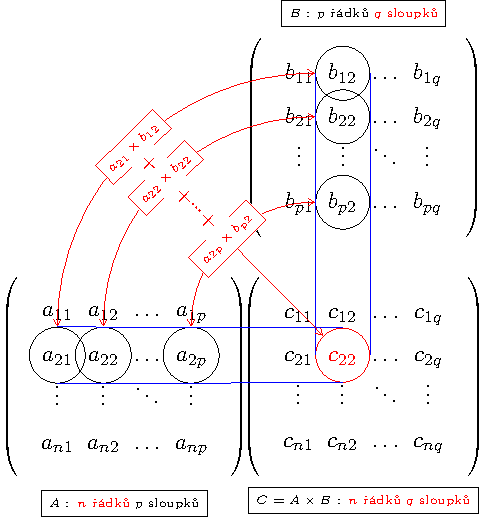
\includegraphics[width=0.45\linewidth]{mai_fig023a}}               &
        \subfloat[2. krok]{\label{LA:fig_LA001b}
          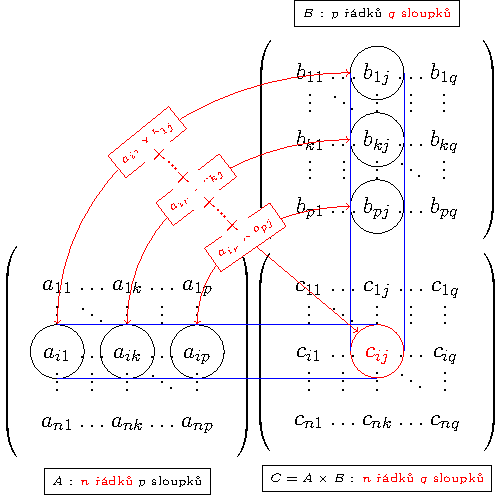
\includegraphics[width=0.45\linewidth]{mai_fig023b}} 
      \end{tabular}
      \caption{Postup při maticovém násobení}
    \end{figure}
  

      
      \begin{definition}\label{rovnost_matic}
       (Rovnost matic):  Matice \(\matr{A} = \left(a_{ij}\right)\) je rovna matici \(\matr{B}=
       \left(b_{kl}\right)\), jsou-li matice stejného typu a stejnolehlé prvky se sobě
       \textbf{rovnají}, tj. \(\matr{A} \in \mathbb{R}_{m,n}, \matr{B}\in\mathbb{R}_{m,n}, 
       a_{ij} = b_{ij}, \forall i\in\lbrace1,2,\ldots,m\rbrace, \forall j\in\lbrace1,2, \ldots 
       ,n\rbrace\).
      \end{definition}
      
%--------------------------------------------------------------------------------------------------
  \section{Počítání s vektory}\label{mai:IchapIIsecIV}
    \textbf{Vektory} budeme nazývat matice typu \(1/n\) a značit je
    \begin{equation*}
      \vec{u} = (u_1, u_2, \ldots, u_n).
    \end{equation*}
    Takže počítat s nimi již umíme! (V zápisu složek vektoru je vynechán řádkový index. V případě 
    matice s jedním řádkem, takzvané \emph{řádkové matice}, je totiž zbytečný.) Číslům \(u_1\) až 
    \(u_n\) budeme pro tuto chvíli říkat \emph{složky vektoru} \(\vec{u}\). Za chvíli tento pojem 
    ještě upřesníme. Celou řadu pojmů, s nimiž jsme se seznámili při počítání s maticemi, můžeme 
    pro vektory přímo použít. Namísto značení \(\mathcal{M} (1/n)\) budeme pro prostor vektorů 
    používat symbol \((\mathbb{R}^n)\) nebo \(\mathbb{C}^n\) (obvyklý symbol pro množinu 
    uspořádaných \(n\)-tic reálných nebo komplexních čísel).
    
    \subsection{Součiny vektorů}
      Kromě základních operací s vektory, tj. sčítání vektorů a násobení vektoru skalárem, se 
      často používají další operace, které obohacují \emph{strukturu vektorového prostoru}. 
      Zůstaneme u vektorů v trojrozměrném prostoru \(\mathbb{R}^3\) a definujeme si skalární, 
      vektorový a smíšený součin vektorů. Skalární součin vektorů definujeme prostřednictvím 
      geometrické definice jako zobrazení, které uspořádané dvojici vektorů (volných vektorů nebo 
      jejich libovolných umístění) přiřazuje reálný číslo podle předpisu
      \begin{equation}\label{mai:eq038}
        \vec{u}\vec{v} = \abs{\vec{u}}\cdot\abs{\vec{v}}\cos\varphi,
      \end{equation}
      kde \(\varphi = \sphericalangle(\vec{u},\vec{v})\) je velikost minimálního z obou úhlů mezi 
      vektory\(\vec{u},\vec{v}\).

    %---------------------------------------------------------------
    % !TeX spellcheck = cs_CZ
% \wikitextrule
\begin{mdframed}[style=mdexam]
  \begin{example}\label{mai:exam034}
    Vypočteme z definice \ref{mai:eq038} skalární součiny vektorů ortonormální báze \(\vec{e_1}\), 
    \(\vec{e_2}\) a \(\vec{e_3}\), spjaté s kartézskou soustavou souřadnic. Připomeňme, že tyto 
    vektory jsou jednotkové a navzájem kolmé.
    \begin{itemize}
      \item pro \(i\neq j\) \(\vec{e_i}\vec{e_j}=0\), 
                \(\sphericalangle\vec{e_i}\vec{e_j} =\dfrac{\pi}{2}\), vektory jsou kolmé,
      \item pro \(i = j\) \(\vec{e_i}\vec{e_j}=0\), 
                \(\sphericalangle\vec{e_i}\vec{e_j} =0, \abs{\vec{e_i}}=1\), vektory jsou 
                jednotkové.
    \end{itemize}

    Pro skalární součiny vektorů ortonormální báze použijeme zkrácené značení
    \begin{equation}\label{mai:eq085}
      \vec{e_i}\vec{e_j} = \delta_{ij},
    \end{equation}
    kde \(\delta_{ij}\) nabývá hodnoty \num{1} pro \(i = j\) a hodnoty \num{0} pro \(i \neq j\). 
    Nazývá se \textbf{Kroneckerovo delta} \cite[s.~40]{Musilova2009MA1}.
  \end{example}
\end{mdframed}
    %---------------------------------------------------------------
    
    Shrneme nyní vlastnosti skalárního součinu. Dokázat bychom je mohli, i když by to mohlo být i 
    velmi pracné, užitím znalostí z goniometrie. Zkuste to alespoň pro jednu z nich! Třeba se    
    vám podaří zvolit si tu nejjednodušší.

%} % tikzset
%---------------------------------------------------------------------------------------------------
\printbibliography[title={Seznam literatury}, heading=subbibliography]
\addcontentsline{toc}{section}{Seznam literatury}
%------------------- Differential calculus --------------------------------------------------------
  % !TeX spellcheck = cs_CZ
% Differential calculus
%{\tikzset{external/prefix={tikz/MAI/}}
% \tikzset{external/figure name/.add={ch03_}{}}
%---------------------------------------------------------------------------------------------------
% Limits_of_Functions.tex
%---------------------------------------------------------------------------------------------------
\chapter{Limita a spojitost funkce}\label{mai:IchapLimit}
\minitoc

  %================Podkapitola: Reálná funkce ======================================================
  \section{Reálná funkce}
    %-----------------------------------------------------------------------------------------------
    \small
    S funkcemi se setkáváme na každém kroku nejen ve fyzice a v ostatních přírodních vědách, ale i 
    v každodenním životě. Každá situace, kdy jsou nějaký jev či veličina jednoznačně a nevyhnutelně 
    určeny jinými jevy či veličinami, se dá popsat pomocí funkce\footnote{V matematice abstrahujeme 
    při zkoumání funkcionálních závislostí od konkrétní fyzikální povahy proměnných veličin a 
    chápeme je jako \uv{bezrozměrné veličiny}, tedy jako číselné proměnné. Někdy je jednoduché 
    takovou} funkci sestavit. Snadno například můžeme zjistit, jakou dráhu urazí automobil jedoucí 
    známou rychlostí v závislosti na tom, jak dlouho jede. Nebo dokážeme určit přírůstek našich 
    úspor ve spořitelně v závislosti na době spoření, pokud známe úrokovou míru a její změny. Jindy 
    je naopak skoro nemožné přijít na to, jak taková funkce vypadá, neboť nemáme dostatek informací 
    o parametrech, které do jejího zápisu vstupují. Třeba takovou závislost teploty ovzduší v daném 
    okamžiku na zeměpisné poloze a nadmořské výšce, kterou bychom si mohli představit jako jednu ze 
    samozřejmých součástí předpovědi počasí, bychom asi nesestavili. Popis jevů pomocí funkcí je v 
    každém případě velmi užitečný. Má však svá pravidla, s nimiž se v této kapitole seznámíme. 
    Závisí-li zkoumaný jev nebo veličina na jediné veličině, jejíž hodnoty jsou reálné a buď se 
    mění známým způsobem, nebo si je můžeme dokonce volit, hovoříme o \textbf{funkci jedné reálné 
    proměnné}. A lze-li zkoumaný jev nebo veličinu kvantifikovat rovněž pomocí reálných hodnot, 
    jedná se o \textbf{reálnou funkci jedné reálné proměnné}. Právě o takových funkcích bude v této 
    kapitole řeč. V aplikacích se budeme věnovat především funkcím, které mají význam ve fyzice a v 
    přírodních vědách. Velmi často půjde o funkce, kde reálnou proměnnou je čas. Jevy v přírodě 
    podléhají totiž principu příčinnosti, a tak lze velké množství veličin popisujících přírodní 
    jevy vyjádřit na základě znalosti přírodních zákonů jako funkce času. 
    \cite[s.~53]{Musilova2009MA1}
    \normalsize
    \subsection{Funkce a její graf}\label{MAI:section_002}
      V tomto odstavci se naučíme funkce zadávat, počítat s nimi a vyjádřit je velmi přehledným 
      způsobem — jejich \emph{grafem}. Zopakujme, že každou \textbf{reálnou funkci}, jejíž 
      definiční obor je podmnožina množiny \(\realset\), nazýváme \textbf{reálnou funkcí jedné 
      reálné proměnné}\footnote{Místo názvu \uv{reálná funkce jedné reálné proměnné} budeme pro 
      stručnost používat pouze název \uv{funkce}, pokud nebude řečeno něco jiného}.
      
      Protože \emph{funkce je speciální případ zobrazení}, můžeme všech\-ny pojmy a obecné 
      vlastnosti zobrazení přenést i na funkce. Některé z nich však vzhledem k důležitosti 
      zopakujme, případně doplníme. Na druhé straně budeme studovat také ty vlastnosti, které jsou 
      specifické pro tento speciální druh zobrazení.
      
      \begin{note}
        Je-li \(\mathcal{D}_f = \naturalset\), jedná se o \textbf{posloupnost}. (Speciálním 
        případem reálných funkcí jedné reálné proměnné jsou \emph{posloupnosti reálných čísel)}.
      \end{note}
      
      \subsection{Způsoby zadání funkce}\label{MAI:section_000}
        Nejprve funkci definujeme. Předpokládejme, že reálná proměnná, na níž bude záviset náš jev, 
        má dovoleno nabývat hodnot z určité předem stanovené podmnožiny \(D\subseteq\realset\) 
        reálných čísel. Předpokládejme dále, že podle určitého pravidla, předpisu, dokážeme pro 
        \emph{každou hodnotu} \(x\) množiny \(\mathcal{D}_f\), tj. \(x \in \mathcal{D}_f\), určit 
        \emph{právě jednu} reálnou hodnotu \(y\). Každé hodnotě \(x \in D\) tedy nějaké \(y\) 
        příslušet \emph{musí},  avšak žádné hodnotě \(x\) \emph{nesmíme} přiřadit více hodnot 
        \(y\). Tak vzniká funkce \(f\). Hodnoty \(x\) se nazývají hodnotami \emph{nezávisle 
        proměnné} (neboli \emph{argumentu}), hodnoty \(y\) hodnotami \emph{závisle proměnné} a 
        \(f\) symbolizuje \emph{funkční předpis}. Píšeme
        \begin{equation}\label{mai:eq000}
            f: x \in \mathcal{D}_f \rightarrow y=f(x)\in\realset
        \end{equation}
      Hodnoty proměnné \(x\) nazýváme též \emph{vzory}, odpovídající hodnoty \(y = f(x)\) 
      \emph{obrazy}. Množina  \(\mathcal{D}_f\) je \emph{definičním oborem} funkce \(f\). Zadání 
      definičního oboru je důležitou součástí zadání funkce. Množina \(H\) všech takových reálných 
      hodnot \(y\), které jsou obrazem nějakého vzoru, 
      \begin{equation}\label{mai:eq001}
          \mathcal{H}_f = 
              \left\lbrace 
                y\in\realset\text{ existuje } x\in \mathcal{D}_f, \text{ tak že } y = f(x)  
              \right\rbrace, 
      \end{equation}
      se nazývá \emph{obor hodnot} funkce \(f\). Hodnotu \(f(x)\) nazýváme také \emph{funkční 
      hodnotou} funkce \(f\) v bodě \(x\). 

      \begin{figure}[ht!] %\ref{mai:fig001}
        \centering
%        % Funkce jako „černá skříňka“. \cite[s.~54]{Musilova2009MA1}

\documentclass[11pt]{standalone}
\usepackage{xltxtra}
\usepackage{tikz}
\usepackage{amsmath}

\begin{document}
  \begin{tikzpicture}[fill=black!20]
%  \draw[help lines] (-1,-2) grid (6,3);
    \path (0,0) node(a) [ ] {\(\mathcal{D}_f\)}
    (2,0) node(b) [rectangle,rotate=0,draw,fill] {\(\begin{array}{c} \text{funkce} \\ f(x)  
    \end{array}\)}
    (4,0) node(c) [ ] {\(\mathcal{H}_f\)};
    \draw[thick,->] (a.east) -- (b);
    \draw[thick,->] (b.east) -- (c);
    \path [ ] (a.east) -- (b.west)   node [above,midway] {\(x\)};
    \path [ ] (b.east) -- (c.west)   node [above,midway] {\(y\)};
  \end{tikzpicture}

\end{document}
        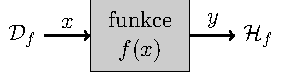
\includegraphics[width=0.45\linewidth]{mai_fig001.pdf}
        \caption{Funkce jako „černá skříňka“. \cite[s.~54]{Musilova2009MA1}}
        \label{mai:fig001}
      \end{figure}
      
      Funkci si podle obrázku \ref{mai:fig001} můžeme představit jako „černou skříňku“, do které 
      vstoupí hodnota (vzor) a vystoupí z ní hodnota \(y = f(x)\) (obraz). Množinu uspořádaných 
      dvojic čísel \([x, f(x)]\) nazveme \hyperref[MAI:section_001]{grafem funkce}.
      
      Jak zadat předpis \(f\)? Lze to udělat kterýmkoli z následujících způsobů, podle vhodnosti
      nebo snadnosti. Ukážeme jednotlivé možnosti na jednoduchém příkladu, kdy chceme hodnotám 
      proměnné \(x\) z množiny \(\mathcal{D}_f\) přiřadit jejich druhé mocniny. Zvolme pro náš 
      příklad definiční obor výčtem:
      \begin{equation*}
         \mathcal{D}_f = \lbrace-3,2,-1,0,1,2,3,4\rbrace,
      \end{equation*}
      a zadáme předpis
      \begin{itemize}\addtolength{\itemsep}{-0.5\baselineskip}
        \item \textbf{slovním popisem}: předpis \(f\) přiřazuje každé z hodnot \(x\in 
              \mathcal{D}_f\) její druhou mocninu,
        \item \textbf{vzorcem}: \(y = x^2\) pro \(x\in \mathcal{D}_f\) zadává zobrazení
              \begin{equation*}
                f: x\in \mathcal{D}_f \rightarrow f(x)= x^2\in\realset,
              \end{equation*}
        \item \textbf{tabulkou}: Hodnoty obrazů pro všechny vzory z \(\mathcal{D}_f\) vypíšeme do 
              tabulky:
              \begin{table}[h]
                \centering
                \begin{tabular}{c|rrrrrrrr}
                  \textbf{x} & -3 & -2 & -1 & 0 & 1 & 2 & 3 & 4  \\ \hline
                  \textbf{y} & 9  & 4  & 1  & 0 & 1 & 4 & 9 & 16
                \end{tabular}
                % \caption{ }
              \end{table}
              Proměnná $x$ se v tomto případě mění \uv{diskrétně}. Je zřejmé, že tímto způsobem 
              můžeme funkci definovat úplně jen tehdy, je-li definiční obor konečná množina. 
              Tabulku však používáme i v jiných případech, zejména chceme-li vyznačit pomocí ní, 
              některé hodnoty, které nás z nějakého důvodu přednostně zajímají. 
        \item Zadání \textbf{grafem}: 
          \begin{equation*}
            G_f = \left\lbrace\left[x,f(x)\right] |x\in D\right\rbrace
                = \left\lbrace\left[x,x^2 \right] |x\in D\right\rbrace
          \end{equation*}
          tak, že dvojice \([x, f(x)]\) znázorníme jako body v rovině (obr. \ref{MAI:fig_011}).
          \begin{figure}[ht!]
            \centering  
            \begin{tabular}{cc}
              \subfloat[ ]{\label{MAI:fig_011}
                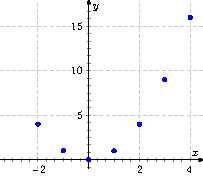
\includegraphics[width=0.4\linewidth]{mai_fig002.pdf}}              &
              \subfloat[ ]{\label{MAI:fig_010}
                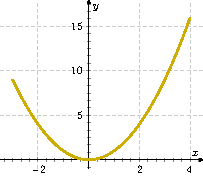
\includegraphics[width=0.4\linewidth]{mai_fig003.pdf}}              \\
            \end{tabular}
            \caption{Zadání funkce grafem}
          \end{figure}
          Z grafu můžeme ovšem funkční hodnoty určit pouze přibližně. Pro další matematické 
          zpracování je grafické zadání nejméně vhodné, i když jeho praktický význam například v 
          technických aplikacích nelze popřít.
        \item Zadání pomocí \textbf{rovnice}, jíž je funkce řešením: některé funkce nelze jednoduše 
              zapsat pomocí některého z předchozích způsobů, nebo to alespoň nejde přesně. Lze však 
              zapsat (diferenciální) rovnici, kterou tato funkce splňuje. Jedná se většinou o 
              speciální funkce, jimž se v tomto textu nebudeme věnovat. (Někdy může být taková 
              rovnice  představující zadání funkce i velmi jednoduchá. Například dosti známá funkce 
              \(\erf(x)\), \emph{error funkce}, velmi úzce souvisí s funkcí \(f(x) = 
              \frac{2}{\sqrt{x}}e^{-x^2}\). Nelze ji však zapsat vzorcem. Některé její hodnoty v 
              nejčastěji používaném rozsahu proměnné \(x\) můžeme najít v rozsáhlých tabulkách, 
              které byly sestaveny pomocí numerických metod.)
      \end{itemize}
      
      Již bylo zmíněno, že zadání definičního oboru je neopominutelnou součástí zadání funkce. 
      Kdybychom například zadali funkci opět předpisem \(y=x^2\), avšak za definiční obor stanovili 
      uzavřený interval \(D = \lbrace —3,4\rbrace\), dostali bychom graf na obrázku 
      \ref{MAI:fig_010}. Jde skutečně o jinou funkci než na obrázku \ref{MAI:fig_011}. Její úplnou 
      tabulku bychom nedokázali napsat vůbec.
      
%      Nejčastější způsob zadání funkce představuje \emph{vzorec}. Tabulku alespoň pro některé 
%      hodnoty z \(\mathcal{D}_f\) si pak dokážeme sestavit a schematický graf nakreslit. Někdy se 
%      objeví zadání funkce jen v podobě vzorce, například: „Je dána funkce \(y = f(x)\).“ Znamená 
%      to, že autor zapomněl zadat definiční obor? Nemusí tomu tak být. Tento způsob zadání chápeme 
%      tak, že si sami musíme stanovit „co největší“ definiční obor této funkce, tj. určit množinu 
%      všech takových \(x\), pro která lze do vzorce dosadit a hodnotu \(y\) určit.

      Zobrazovací předpis, kterým je funkce zadána, může být rozmanitý. Nejčastěji a pro účely 
      matematické analýzy nejvhodnější je \emph{analytické zadání vzorcem}, tj. rovnicí tvaru 
      $y=f(x)$ nebo několika takovými rovnicemi platnými pro různé části definičního oboru. Přitom 
      v rovnici $y=f(x)$ je na pravé straně nějaký správně definovaný výraz obsahující nejvýše 
      proměnnou $x$ a nabývající jednoznačné hodnoty pro danou hodnotu proměnné $x$.
      
%      Někdy však používáme (poněkud nedůsledně) termíny \uv{funkce \(f(x)\)} nebo \uv{funkce 
%      \(y=f(x)\)}. V tomto smyslu nepojímáme již \(x\) jako pevný prvek z definičního oboru, ale 
%      jako \uv{nezávisle proměnnou} neboli \emph{argument}, tj. symbol zastupující libovolný prvek 
%      z definičního oboru. V tomto případě pak písmeno \(y\) v rovnici \(y=f(x)\) nazýváme 
%      \emph{závisle proměnnou} a říkáme, že \uv{\(y\) závisí na \(x\)}. Tato frazeologie má své 
%      historické kořeny; tento způsob vyjádření funkce budeme využívat zřídka, zejména tam, kde 
%      nechceme pro označení příslušné funkce zavádět zvláštní symbol. Tak např. budeme mluvit o 
%      funkci \(e^x\) (ačkoliv se zavádí pro exponenciální funkci symbol exp) nebo o funkci \(\sin 
%      x\) (ačkoliv by bylo důslednější mluvit o funkci \(\sin\)) apod. \cite[s.~82]{Brabec1989} 

    %-------------------------------------
      % !TeX spellcheck = cs_CZ
\begin{mdframed}[style=mdexam]
  \begin{example}\label{MAI:exam017}
    (Definiční obor a obor hodnot funkce): Určíme „co největší“ definiční obor funkce
    \(y=\log_2{(\sqrt{1-x^2})}\) a zjistíme také její obor hodnot.
        
    {\centering
    \captionsetup{type=figure}
  %   % !TeX spellcheck = cs_CZ
% exam017.tex
% K příkladu \ref{fyz:fey_exam017} \(y=\log_2{(\sqrt{1-x^2})}\) 

\documentclass[11pt]{standalone}
\usepackage{xltxtra}
\usepackage[usenames,x11names]{xcolor}
\usepackage{tikz}
\usepackage{pgfplots}
  \pgfplotsset{compat=newest}
\usepackage{amsmath}

\begin{document}
  \begin{tikzpicture}[thick,scale=0.7, every node/.style={transform shape}]
    \begin{axis}[
      xmin = -1, xmax = 1, ymin = -10, ymax = 0,
      domain = -0.999999:0.999999,
      restrict y to domain=-30:0,
      grid = major,   % both
      grid style={line width=.1pt, draw=gray!20},
      major grid style={dashed, line width=.2pt, draw=gray!40},
      minor tick num=5,
      clip = true,
      clip mode=individual,
      axis x line = middle,
      axis y line = middle,
      xlabel={\(x\)},
    %  xlabel style={at=(current axis.right of origin), anchor=west},
      ylabel={\(y\)},
    %  ylabel style={at=(current axis.above origin), anchor=south},
      enlarge y limits={rel=0.13},
      enlarge x limits={rel=0.07},
    ]
    
     \addplot[color=Gold3, samples=1000, smooth, ultra thick, unbounded coords=jump, no markers] 
        gnuplot{log10(sqrt(1-x^2))/log10(2)};  
    \end{axis}
  \end{tikzpicture}

\end{document}

% note: předchozí varianta MAI013
%\begin{tikzpicture}
%    \begin{axis}[
%        axis lines=middle,
%        width=10cm, height=10cm,     % size of the image
%        grid = both,
%        grid style={dashed, gray!30},
%        enlargelimits=true,
%        xmin=-1,      % start the diagram at this x-coordinate
%        xmax= 1,      % end   the diagram at this x-coordinate
%        ymin= -6,     % start the diagram at this y-coordinate
%        ymax= 0.5,     % end   the diagram at this y-coordinate
%        /pgfplots/xtick={-1,-0.5,...,1},   % make steps of length 0.2
%        /pgfplots/ytick={0,-0.5,...,-6},   % make steps of length 0.1
%        axis background/.style={fill=white},
%        axis line style={thick, shorten >=2pt, ->, > = {Latex[scale=1.3]}},
% %       every axis x label/.style={
% %        at={(ticklabel* cs:1.0)},
% %        anchor=west,
% %       },
% %       every axis y label/.style={
% %        at={(ticklabel* cs:1.0)},
% %        anchor=south,
% %       },
%        every axis x label/.style={at={(current axis.right of origin)},anchor=west},
%        every axis y label/.style={at={(current axis.north)},above=0mm},
%        ylabel=\(y\),
%        xlabel=\(x\),
% %       title={Dirichletova funkce}
%      ]
%      \addplot[domain=-0.9999:0.9999, line width=0.5pt,samples=1000,red]{log2(sqrt(1-x^2))};
%    \end{axis} 
%\end{tikzpicture}
    \luafigure[0.9]{mai_fig004.pdf}
    \captionof{figure}{K příkladu \ref{MAI:exam017} \(y=\log_2{(\sqrt{1-x^2})}\) 
    \cite[s.~57]{Musilova2009MA1}
    \label{mai:fig004}}
    \par}
    
    Využijeme našich znalostí ze střední školy. Ve hře jsou tři funkce: logaritmus, odmocnina a
    kvadratická funkce, postupně: 
    \begin{equation*}
      y = \log_2w, \qquad w = \sqrt{u}, \qquad u = 1 - x^2.
    \end{equation*}
    „Největším“ definičním oborem logaritmu je množina \(\mathcal{D}(log) = {w\realset \mid w >
    0}\). Oborem hodnot logaritmu pro \(w \in \mathcal{D}(log)\) je celá reálná osa. Hodnoty \(w\)
    však dostáváme vyčíslením odmocniny, která pro přípustné hodnoty \(u\), \(\mathcal{D}(\sqrt{ })
    = \lbrace u\in\realset \lvert u\geq 0\rbrace\), může nabývat všech nezáporných hodnot, tj.
    kladných a hodnoty nula (té nabývá pro \(u = 0\)). Hodnotu \(w = 0\) však nesmíme do logaritmu
    dosadit, takže hodnotu \(u = 0\) musíme ihned vyloučit. Hodnoty proměnné \(x\) musíme omezit
    tak, aby kvadratická funkce \(u = 1 - x^2\) nabývala pouze kladných hodnot. Dostáváme tak
    definiční obor funkce \(y = f(x)\) \(\mathcal{D}=\lbrace x\in\realset \lvert -1<x<1\rbrace\),
    neboli otevřený interval \((-1, 1)\). Pro \(x \in \mathcal{D}\) pak funkce \(u(x)\) nabývá
    hodnot v intervalu \(\mathcal{H}_u = \left( 0, 1\right]\) a funkce \(\log_2\sqrt{1-x^2}\) hodnot
    v intervalu \(\mathcal{H}_u = \left( -\infty, 0\right]\), který je tedy jejím oborem hodnot.
    Graf funkce vidíme na obr. \ref{mai:fig004}. 
  \end{example}
\end{mdframed}
    %-----------------------------------------------------------------------------------------------
    \subsection{Graf funkce}\label{MAI:section_001}\hypertarget{MAI:section_001}
      Jinými slovy, v předchozím odstavci, bylo řečeno, že každé funkci můžeme přiřadit její graf, 
      a že \textbf{grafem funkce} $f:A\rightarrow\realset,\ A\subset\realset$, rozumíme množinu 
      všech bodů euklidovské roviny, jejíž souřadnice $x$, $y$ v dané kartézské soustavě souřadnic 
      vyhovuje rovnice 
      \begin{equation}\label{mai:eq026}
        y=f(x). 
      \end{equation}  
      
      Graf funkce může v jednodušších případech posloužit jako prostředek k získání názorné 
      \uv{představy}. Grafy některých funkcí jsou \uv{křivky}, (intuitivním smyslu tohoto slova). 
      Avšak u některých funkcí názorná představa grafu selhává. Vezmeme-li např. Dirichletovu 
      funkci, snadno zjistíme, že její graf nemůžeme sestrojit (obr. \ref{mai:fig005} tedy 
      není grafem funkce, ale pouze pokusem o názorné přiblížení Dirichletovi funkce)
      
      \begin{figure}[ht!] %\ref{mai:fig005}
        \centering
%       % !TeX spellcheck = cs_CZ
%
% Pokus o zobrazení Dirichletovy funkce: \uv{dvě rovnoběžné přímky $y=0$ a $y=1$ s 
% nekonečným množstvím mezer}
% xelatex -enable-write18 -shell-escape mai_fig005.tex

\documentclass[11pt]{standalone}
\usepackage{xltxtra}
\usepackage[usenames,x11names]{xcolor}
\usepackage{tikz}
\usepackage{pgfplots}
  \pgfplotsset{compat=newest}
\usepackage{amsmath}
\usepackage{amsfonts}           % \mathbb{Q}
\usepackage{tabularx}           % \shortstack

\begin{document}
  \begin{tikzpicture}[thick,scale=0.7, every node/.style={transform shape}]
    \begin{axis}[
      xmin = -3, xmax = 3, ymin = 0, ymax = 2,  % osy
      domain = -3:3,
      restrict y to domain=0:4,
      grid = major,   % both
      grid style={line width=.1pt, draw=gray!20},
      major grid style={dashed, line width=.2pt, draw=gray!40},
      minor tick num=5,
      clip = true,
      clip mode=individual,
      axis x line = middle,
      axis y line = middle,
      xlabel={\(x\)},
    %  xlabel style={at=(current axis.right of origin), anchor=west},
      ylabel={\(y\)},
    %  ylabel style={at=(current axis.above origin), anchor=south},
      enlarge y limits={rel=0.13},
      enlarge x limits={rel=0.07},
    %  title={Dirichletova funkce}
    ]
        
        \addplot[domain=-3:3, ultra thick,samples=10,blue] {1};
        \label{plot one}
        \addplot[domain=-3:3, ultra thick,samples=10,red] {0};
        \label{plot two} 
        \node [draw,fill=white] at (rel axis cs: 0.6,0.7) {\shortstack[l]{
        \(f(x) = 
          \left\lbrace\begin{array}{l@{}l@{}}
              1 & \text{ když } x \in  \mathbb{Q}\\
              0 & \text{ když } x \in  \mathbb{R} \setminus\mathbb{Q}
          \end{array}\right.
       \)
          }
           };
      \end{axis} 
  \end{tikzpicture}
\end{document}
        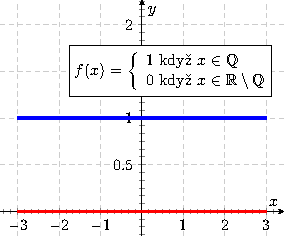
\includegraphics[width=0.5\linewidth]{mai_fig005.pdf}
        \caption{Pokus o zobrazení Dirichletovy funkce: \uv{dvě rovnoběžné přímky $y=0$ a $y=1$ s 
        nekonečným množstvím mezer}}
        \label{mai:fig005}
      \end{figure}      
      Z předchozí kapitoly také víme, že zadat funkci znamená udat její definiční obor a 
      \uv{zobrazovací předpis}, tj pravidlo (formulované slovně či v používaném matematickém 
      jazyku), podle něhož můžeme jednoznačným způsobem rozhodnout, jaká funkční hodnota odpovídá 
      libovolně zvolenému číslu z definičního oboru. Definičním oborem bývá často interval nebo 
      sjednocení intervalů. Není-li definiční obor udán, rozumíme jím množinu všech reálných čísel, 
      pro něž je příslušný předpis definován. Tuto množinu nazýváme \textbf{přirozeným} (též 
      maximálním) definičním oborem funkce. Je to tzv. \emph{existenční obor} výrazu, jímž je 
      funkce definována \cite[s.~84]{Brabec1989}.
      
      Například funkce $f: \realset\rightarrow\realset,\ f(x)=x^2$, můžeme vyjádřit bez udání 
      definičního oboru $\realset$ vztahem 
      \begin{equation*}
        f: y=x^2,
      \end{equation*}
      neboť předpis $y=x^2$ má smysl pro každé reálné číslo $x$. Avšak u funkce $g:\langle0, 
      1\rangle\rightarrow\realset,\ g(x)=x^2,$ je nutné v zápisu funkce definiční obor $\langle0, 
      1\rangle$ 
      uvést, píšeme tedy   
      \begin{equation*}
        g: y=x^2, \quad x\in\langle0,1\rangle.
      \end{equation*}
       
      %-------------------------------------
        % !TeX spellcheck = cs_CZ
\wikitextrule
\begin{example}\label{MAI:exam018} 
  Vzorcem $f(x)=\sqrt{1-x}$ je dána funkce, jejímž přirozeným oborem je interval 
  $(-\infty,1\rangle$ (uvažme, že výraz $\sqrt{1-x}$ je definován v reálném oboru, je-li 
  $1-x\geq0$). Graf této funkce je část paraboly, jejíž osou je osa $x$, viz obr. 
  \ref{mai:fig006}.
  
  {\centering
   \captionsetup{type=figure}
%  % !TeX spellcheck = cs_CZ
% mai_fig006.tex

\documentclass[11pt]{standalone}
\usepackage{xltxtra}
\usepackage[usenames,x11names]{xcolor}
\usepackage{tikz}
\usepackage{pgfplots}
  \pgfplotsset{compat=newest}
\usepackage{amsmath}


\begin{document}
  \begin{tikzpicture}[thick,scale=0.7, every node/.style={transform shape}]
    \begin{axis}[
      xmin = -3, xmax = 1.5, ymin = 0, ymax = 3,  % osy
      domain = -3:1,
      restrict y to domain=0:4,
      grid = major,   % both
      grid style={line width=.1pt, draw=gray!20},
      major grid style={dashed, line width=.2pt, draw=gray!40},
      minor tick num=5,
      clip = true,
      clip mode=individual,
      axis x line = middle,
      axis y line = middle,
      xlabel={\(x\)},
    %  xlabel style={at=(current axis.right of origin), anchor=west},
      ylabel={\(y\)},
    %  ylabel style={at=(current axis.above origin), anchor=south},
      enlarge y limits={rel=0.13},
      enlarge x limits={rel=0.07},
    ]
    
     \addplot[color=Gold3, samples=200, smooth, ultra thick, unbounded coords=jump, no markers] 
        gnuplot{sqrt(1-x)};  
    \end{axis}
  \end{tikzpicture}
\end{document} 
   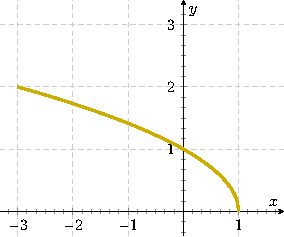
\includegraphics[width=0.5\linewidth]{mai_fig006.pdf}
   \captionof{figure}{{Graf funkce $y=\sqrt{1-x}$ je část paraboly, jejíž hlavní osou je osa $x$}}
   \label{mai:fig006}
   \par}

\end{example}
      %-------------------------------------
      
      %-------------------------------------
        % !TeX spellcheck = cs_CZ
\begin{mdframed}[style=mdexam]
  \begin{example}\label{MAI:exam019} 
    Funkce je dána vzorcem 
    \begin{equation*}
      f(x):y=\abs{x}.
    \end{equation*} 
    Přirozeným definičním oborem této funkce je množina $\realset$. Táž funkce může být dána i 
    vzorcem
    \begin{equation*}
      f(x):y=\sqrt{x^2},
    \end{equation*}    
    nebo dvěma rovnicemi
    \begin{equation*}
      f(x):y=
        \begin{cases}
             x & \text{je-li} x \geq 0. \\
            -x & \text{je-li} x < 0,
        \end{cases}                 
    \end{equation*}  
    což je zřejmé, uvědomíme-li si jak je definována absolutní hodnota. Graf funkce je na obr. 
    \ref{mai:fig007}.
    
    {\centering
    \captionsetup{type=figure}
  %  % !TeX spellcheck = cs_CZ
% mai_fig007.tex

\documentclass[11pt]{standalone}
\usepackage{xltxtra}
\usepackage[usenames,x11names]{xcolor}
\usepackage{tikz}
\usepackage{pgfplots}
  \pgfplotsset{compat=newest}
\usepackage{amsmath}

\begin{document}
  \begin{tikzpicture}[thick,scale=0.7, every node/.style={transform shape}]
    \begin{axis}[
      xmin = -3, xmax = 3, ymin = 0, ymax = 3,  % osy
      domain = -3:3,
      restrict y to domain=0:3,
      grid = major,   % both
      grid style={line width=.1pt, draw=gray!20},
      major grid style={dashed, line width=.2pt, draw=gray!40},
      minor tick num=5,
      clip = true,
      clip mode=individual,
      axis x line = middle,
      axis y line = middle,
      xlabel={\(x\)},
    %  xlabel style={at=(current axis.right of origin), anchor=west},
      ylabel={\(y\)},
    %  ylabel style={at=(current axis.above origin), anchor=south},
      enlarge y limits={rel=0.13},
      enlarge x limits={rel=0.07},
    ]
    
     \addplot[color=Gold3, samples=200, smooth, ultra thick, unbounded coords=jump, no markers] 
        gnuplot{abs(x)};  
    \end{axis}
  \end{tikzpicture} 
\end{document}
    \luafigure[0.9]{mai_fig007.pdf}
    \captionof{figure}{Graf funkce $y=\abs{x}$}
    \label{mai:fig007}
    \par}
  \end{example}
\end{mdframed}
      %-------------------------------------
      
      Funkce může být analyticky zadána i jinak než vzorcem $y=f(x)$. Časté je \textbf{parametrické 
      vyjadřování}, tj. vyjádření dvojicí rovnic 
      \begin{equation}\label{mai:eq027}
        x=\varphi(t),\ y=\psi(t),\ t\in J,
      \end{equation}
      kde $\varphi, \psi$ jsou funkce definované na množině $J$ ($\ J$ bývá obvykle interval). 
      Proměnná $t$ se nazývá \emph{parametr}: má zde pomocný význam. Zajímá nás totiž vztah mezi 
      $x$ a $y$. Rovnice \ref{mai:eq027} definuje relaci 
      $f\subset\realset\times\realset=\realset^2$:
      \begin{equation*}
        f = \{(x,y)\in\realset^2; \text{ existuje } t\in J \text{ tak, že } x=\varphi(t),\ y=\psi(t)\}.
      \end{equation*}      
      Tato relace může být za \emph{určitých podmínek jednoznačná} tj. je funkcí z $\realset$ do 
      $\realset$. V tomto případě říkáme, že funkce $f$ je \emph{definována parametricky rovnicemi 
      \ref{mai:eq027}}
      
      %-------------------------------------
        % !TeX spellcheck = cs_CZ
\begin{mdframed}[style=mdexam]
  \begin{example}\label{mai:exam020} 
    Rovnice $x=\cos t,\ y=\sin t\quad t\in\langle0,\pi\rangle$, definují parametricky funkci 
    \begin{equation}
      f: y= \sqrt{1-x^2}, \quad x\in\langle-1,1\rangle,
    \end{equation}
    jejíž grafem je polokružnice, ležící v horní polorovině $\{(x,y)\in\realset^2, y\geq0\}$.
    
    {\centering
    \captionsetup{type=figure}
  %   % !TeX spellcheck = cs_CZ
%Graf funkce \(y=\sqrt{1-x^2}\) je polokružnice

\documentclass[11pt]{standalone}
\usepackage{xltxtra}
\usepackage[usenames,x11names]{xcolor}
\usepackage{tikz}
\usepackage{pgfplots}
  \pgfplotsset{compat=newest}
\usepackage{amsmath}

\begin{document}
  \begin{tikzpicture}[thick,scale=0.7, every node/.style={transform shape}]
    \begin{axis}[
      xmin = -1.2, xmax = 1.2, ymin = 0, ymax = 1.3,  % osy
      domain = -1:1,
      restrict y to domain=0:1,
      unit vector ratio=1 1 1,  % axis equal
      grid = major,   % both
      grid style={line width=.1pt, draw=gray!20},
      major grid style={dashed, line width=.2pt, draw=gray!40},
      minor tick num=5,
      clip = true,
      clip mode=individual,
      axis x line = middle,
      axis y line = middle,
      xlabel={\(x\)}, ylabel={\(y\)},
      enlarge y limits={rel=0.07},
      enlarge x limits={rel=0.07},
    ]
    
      \addplot[color=Gold3, samples=200, smooth, ultra thick, unbounded coords=jump, no markers] 
         gnuplot{sqrt(1-x^2)};  
    \end{axis}
  \end{tikzpicture} 
\end{document}
    \luafigure[0.9]{mai_fig008.pdf}
    \captionof{figure}{Graf funkce \(y=\sqrt{1-x^2}\) je polokružnice}
    \label{mai:fig008}
    \par}
  \end{example}
\end{mdframed}
      %-------------------------------------
      
      Blíže se parametrickým zadáním funkce budeme zabývat v kapitole \ref{chap:Apl_dif_poc}
      (Aplikace diferenciálního počtu).
      
      Funkce může být někdy zadána též rovnicí tvaru 
      \begin{equation}\label{mai:eq028}
        F(x,y) = 0.
      \end{equation}
      Přitom $F$ je funkce dvou proměnných, tj. zobrazení z $\realset^2\rightarrow\realset$. Kromě 
      rovnice \ref{mai:eq028} může být dána ještě podmínka, aby bod $(x,y)$ patřil k některé 
      množině $M\subset\realset^2$. Rovnicí \ref{mai:eq028} je definována opět jakási relace 
      $f\subset\realset\times\realset$,
      \begin{equation}
        f = \{(x,y)\in\realset^2,\quad F(x,y)=0 \}
      \end{equation}
      (případně $f = \{(x,y)\in\realset^2,\ F(x,y)=0,\ (x,y)\in M \}$), zajímá nás, kdy tato relace 
      je funkcí z $\realset$ do $\realset$. Říkáme pak, že funkce $f$ je dána \textbf{implicitně} 
      uvedenou rovnicí \ref{mai:eq028} (příp. rovnicí \ref{mai:eq028} a podmínkou $(x,y)\in 
      M$). Naproti tomu zadání funkce ve tvaru $y=f(x)$ nazýváme \textbf{explicitním}.

      %-------------------------------------
        % !TeX spellcheck = cs_CZ
\begin{mdframed}[style=mdexam]
  \begin{example}\label{MAI:exam022}\todo[inline]{Nedokončený příklad}
    \begin{itemize}
    \item[]
    \item  Rovnicí $x+2y-3=0$ je implicitně definována funkce  
          $f:y=-\dfrac{1}{2}x+\dfrac{3}{2}$.
    \item  Rovnicí $x^2+y^2=1$ a podmínkou $y\geq0$ je definována implicitní funkce z příkladu 
          \ref{MAI:exam020}. Relace $\{(x,y)\in\realset^2;\ x^2+y^2=1\}$ není ovšem jednoznačná, 
          každé hodnotě $x\in(-1,1)$ odpovídají dvě hodnoty $y: y_1=\sqrt{1-x^2}$, $y: y_2 = 
          -\sqrt{1-x^2}$. Podmínkou $y\geq0$ druhou hodnotu vylučujeme. Místo podmínky $y\geq0$ 
          bychom mohli uvést i jiné podmínky, aby rovnice $x^2+y^2=1$ určovala implicitní funkci.   
    \end{itemize}
  \end{example}
\end{mdframed}
      %-------------------------------------
      
      Vyšetřování podmínek, při nichž rovnice $F(x,y)=0$ je definována funkce $f$, se obvykle 
      provádí metodami matematické analýzy funkce více proměnných. 
          
    %---------------------------------------------------------------------------------------------- 
    \subsection{Vlastnosti funkcí}\label{MA1:subsec_vlastnosti_funkce}
      \subsubsection{Omezená funkce}
        \begin{definition}\label{MA1:def_lim01}
          Funkci $f$ nazýváme shora (zdola) omezenou na množině $A\subset D(f)$, je-li shora 
          (zdola) omezená množina funkčních hodnot $f(A)$. Je-li funkce $f$ omezená shora i zdola 
          na množině $A$, pak ji nazýváme omezenou na množině $A$. Je-li $A=D(f)$, nazýváme funkci 
          omezenou. Viz kniha \cite[s.~87]{Brabec1989}       
        \end{definition}
        Funkce \(f\) je omezená na množině \(A\), právě když existuje číslo \(K>0\) tak, že platí
        \begin{align*}
         |f(x)|      &\leq K \qquad \text{pro každé } x\in A   \\ 
         \shortintertext{neboli}
         -K\leq f(x) &\leq K \qquad \text{pro každé } x\in A. 
        \end{align*}

        %-------------------------------------
          % !TeX spellcheck = cs_CZ
\wikitextrule
\begin{example}\label{MAI:exam023}
  Funkce $f:y=\dfrac{1}{x^2+1}$ je omezená. Platí totiž 
  \begin{equation*}
    \left|\frac{1}{x^2+1}\right|=\frac{1}{x^2+1}\leq1 \qquad \text{pro všechna }x\in\realset.
  \end{equation*}
  Zdola je tato funkce omezena dokonce číslem $0$.  
\end{example}
        %-------------------------------------

        \begin{itemize}\addtolength{\itemsep}{-0.5\baselineskip}
          \item Je-li funkce $f$ shora omezená na množině $A$, existuje konečné \emph{supremum}     
                $\sup f(A)$. Toto číslo nazýváme \emph{supremem funkce $f$ na množině $A$} a 
                označujeme je též $\sup_{x\in A}f(A)$ nebo $\sup\{f(x), x\in A\}$.
          \item Je-li funkce $f$ zdola omezená na množině $A$, existuje konečné \emph{infimum} 
                $\inf(A)$, které nazýváme \emph{infimum funkce $f$ na množině $A$} a označujeme je 
                též $\inf_{x\in A}f(A)$ nebo $\inf\{f(x), x\in A\}$. 
          \item Není-li funkce $f$ shora (zdola) omezená na množině $A$, pak je ovšem $\sup_{x\in A}
                f(x)=+\infty$ ($\sup_{x\in A} f(x)=-\infty$).
          \item Má-li množina $f(A)$ největší (nejmenší) prvek, pak toto číslo nazýváme největší 
                (nejmenší hodnotou funkce $f$  na množině $A$ (je-li $A = f(f)$, též absolutním 
                maximem, resp. absolutním minimem funkce $f$) a značíme je $\max_{x\in A} f(x)$ 
                ($\min_{x\in A} f(x)$). V tomto případě existuje takové číslo $x_0\in A$, že 
                $f(x_0)=\max_{x\in A}f(x)$ ($f(x_0)=\min_{x\in A}f(x)$). Pro všechna $x\in A$ tedy 
                platí $f(x)\leq f(x_0)$ ($f(x)\geq f(x_0)$). Je zřejmé, že největší (nejmenší) 
                hodnota funkce $f$ na množině $A$, pokud existuje je současně supremem (infimem) 
                funkce $f$ na $A$.
        \end{itemize}

      %-------------------------------------
        % !TeX spellcheck = cs_CZ
\wikitextrule
\begin{example}\label{MAI:exam021} 
  Pro funkci z příkladu \ref{MAI:exam023} platí:
  \begin{align*}
    \sup_{x\in\realset}&=\frac{1}{x^2+1}=\max_{x\in\realset}=\frac{1}{x^2+1}=1;   \\
    \inf_{x\in\realset}&=\frac{1}{x^2+1}=0,
  \end{align*}
  tato funkce však nenabývá v definičním oboru $\realset$ nejmenší hodnoty, neboť je stále 
  $\dfrac{1}{x^2+1}>0$. To, že infimum je $0$, dokážeme takto: Zvolíme-li libovolně 
  $\varepsilon>0$, pak snadno zjistíme, že existuje $x$, pro něž 
  $\dfrac{1}{x^2+1}<\varepsilon$:
  \begin{align*}
    1                  &< \varepsilon(x^2+1) \\
    \frac{1}{\epsilon} &< x^2+1 \Rightarrow \sqrt{\frac{1}{\epsilon}-1} < x
  \end{align*} 
  
  {\centering
   \captionsetup{type=figure}
%   % !TeX spellcheck = cs_CZ
%Graf funkce $f(x):y=\dfrac{1}{1+x^2}$

\documentclass[11pt]{standalone}
\usepackage{xltxtra}
\usepackage[usenames,x11names]{xcolor}
\usepackage{tikz}
\usepackage{pgfplots}
  \pgfplotsset{compat=newest}
\usepackage{amsmath}

\begin{document}
  \begin{tikzpicture}[thick,scale=0.7, every node/.style={transform shape}]
    \begin{axis}[
      xmin = -4.2, xmax = 4.5, ymin = 0, ymax = 1.3,  % osy
      domain = -4:4,
      restrict y to domain=0:1,
  %    unit vector ratio=1 1 1,  % axis equal
      grid = major,   % both
      grid style={line width=.1pt, draw=gray!20},
      major grid style={dashed, line width=.2pt, draw=gray!40},
      minor tick num=5,
      clip = true,
      clip mode=individual,
  %    /pgfplots/xtick={-2,-1,1,2}, % make steps of length 0.2
      axis x line = middle,
      axis y line = middle,
      xlabel={\(x\)}, ylabel={\(y\)},
      enlarge y limits={rel=0.07},
      enlarge x limits={rel=0.07},
    ]
    
      \addplot[color=Gold3, samples=200, smooth, ultra thick, unbounded coords=jump, no markers] 
         gnuplot{1/sqrt(1+x^2)};  
    \end{axis}
  \end{tikzpicture}
\end{document} 
   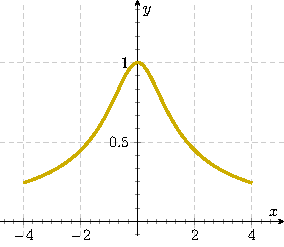
\includegraphics[width=0.5\linewidth]{mai_fig009.pdf}
   \captionof{figure}{Graf funkce $f(x):y=\dfrac{1}{1+x^2}$}
   \label{mai_fig009}
  \par}
  
  Neexistuje tedy kladné číslo, jež by bylo dolní mezí množiny funkčních hodnot, takže infimum je 
  $0$. Graf funkce $f$ je na obr. \ref{mai_fig009}.
\end{example}
      %-------------------------------------
       
      \subsubsection{Monotonní funkce}
        \begin{definition}\label{MA1:def_lim02}
          Funkci $f$ nazýváme \textbf{rostoucí (klesající)} na množině $A\subset D(f)$, jestliže 
          pro každé dva body $x_1, x_2\in A,\ x_1<x_2$, platí $f(x_1)<f(x_2)$ ($f(x_1)>f(x_2)$). 
          Funkci $f$ nazýváme \textbf{neklesající (nerostoucí)} na množině $A\subset D(f)$, 
          jestliže pro každé dvě body $x_1, x_2\in A,x_1<x_2$, platí $f(x_1)\leq f(x_2)$ 
          ($f(x_1)\geq f(x_2)$). Rostoucí a klesající funkce (na množině $A$) se nazývají 
          \textbf{ryze monotónní} (na množině $A$), neklesající a nerostoucí funkce (na množině 
          $A$) se nazývají monotónní (na množině $A$).    
        \end{definition}
            
        Z definice je zřejmé, že každá rostoucí funkce je zároveň neklesající a každá klesající 
        funkce je zároveň nerostoucí. Ryze monotónní funkce tvoří tedy podmnožinu množiny 
        monotónních funkcí. 
           
        \begin{example}
          Funkce $y=2x+1$ je \textbf{rostoucí} na intervalu $(-\infty, \infty)$. Platí totiž: $x_1<x_2\Rightarrow 2x_1<2x_2\Rightarrow2x_1+1<2x_2+1$.
        \end{example}
        \begin{example}
          Funkce y=[x] je \textbf{neklesající} na intervalu $(-\infty, \infty)$ (viz příklad **). 
        \end{example}
        \begin{example}
          Heavisideova funkce (viz příklad **) je \textbf{neklesající} na intervalu $(-\infty, \infty)$ (viz příklad **). 
        \end{example}       
        \begin{example}
          Funkce $y=|x|$ je \textbf{klesající} na intervalu $(-\infty, 0\rangle$ a rostoucí na intervalu $\langle0, \infty)$. 
        \end{example}  
            
        \begin{definition}\label{MA1:def_lim03}
          Funkci $f$ nazýváme \textbf{konstantní} na množině $A$, jestliže pro každé dva body $x_1, 
          x_2\in A$, platí $f(x_1)=f(x_2)$. V tom případě existuje reálné číslo $k$ takové, že pro 
          každé $x\in A$ je $f(x)=k$. Je-li $k=0$, mluvíme o nulové funkci na množině $A$. 
        \end{definition} 
          
        Výrok \uv{funkce $f$ je konstantní na množině $A$} zapisujeme též $f(x)=\text{konst na }A$. 
        Funkci konstantní na $\realset$ budeme stručně nazývat \textbf{konstantní funkcí} nebo 
        krátce \textbf{konstantou}. Z textu bude obvykle patrno, interpretujeme-li symbol $k$ jako 
        reálné číslo nebo jako konstantní funkci. Je zřejmé, že konstantní funkce na množině $A$ je 
        zároveň neklesající i nerostoucí na množině $A$. Toto tvrzení se dá obrátit. Lze snadno 
        dokázat i tuto větu:        
        \begin{lemma}\label{MA1:lem_lim01}
          Funkce $f$ je \textbf{rostoucí} na množině $A$, právě když je neklesající na množině $A$ a na žádné dvoubodové podmnožině $B\subset A$ není konstantní. 
        \end{lemma}
        Obdobná tvrzení platí i pro klesající funkce. 
               
      \subsubsection{Sudé a liché funkce}
        \begin{definition}\label{MA1:def_lim04}
          Funkce $f$ se nazývá \textbf{sudá} jestliže pro každé $x\in D(f)$ je též $-x\in D(f)$  a 
          platí $f(x)=f(-x)$.
          Funkce $f$ se nazývá \textbf{lichá} jestliže pro každé $x\in D(f)$ je též $-x\in D(f)$  a 
          platí $f(-x)=-f(x)$. 
        \end{definition}
        Graf sudé funkce je souměrný podle osy $y$ (osy funkčních hodnot), graf liché funkce je  
        souměrný podle počátku. 
 
       %-------------------------------------
         % !TeX spellcheck = cs_CZ
\wikitextrule
\begin{example}\label{MAI:exam024} 
  Funkce $f:\,y=x^2$ je sudá, funkce $g:\,y=x^3$ je lichá.
  
  {\centering
   \begin{tabular}{cc}
     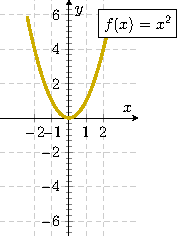
\includegraphics[width=0.5\linewidth]{mai_fig010.pdf}              &
     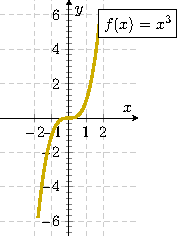
\includegraphics[width=0.5\linewidth]{mai_fig011.pdf}             \\
  \end{tabular}
  \captionsetup{type=figure}
  \captionof{figure}{Příklad sudé a liché funkce}\label{MAI:fig_002}
  \par}
\end{example}
       %-------------------------------------

        Daná funkce nemusí být ovšem ani sudá, ani lichá. Snadno se dokáže tvrzení:
        \begin{itemize}
          \item Je-li sudá funkce $f$ na množině $D(f)\cap\langle0,\infty)$ rostoucí (klesající),
                je na množině $D(f)\cap(-\infty,0\rangle$ klesající (rostoucí).
          \item Je-li lichá funkce na množině $D(f)\cap\langle0,\infty)$ rostoucí (klesající),
                je též na množině $D(f)\cap(-\infty,0\rangle$ klesající (rostoucí).                 
        \end{itemize}
      \subsubsection{Periodická funkce}

    \subsection{Operace s funkcemi. Uspořádání}
      Jak s funkcemi počítat? Definujeme základní operace s nimi — \emph{součet funkcí, součin 
      funkcí a násobení funkce reálným číslem}. Předpokládejme, že na definičním oboru 
      \(\mathcal{D}\) jsou zadány funkce \(f\) a \(g\) a reálné číslo \(\alpha\). Pak na tomtéž 
      definičním oboru lze zadat nové funkce
      \begin{align*}
        \mathcal{F} &: \mathcal{D}\ni x\,\rightarrow\,\mathcal{F}(x) = f(x)+g(x)  \in\realset   \\
        \mathcal{G} &: \mathcal{D}\ni x\,\rightarrow\,\mathcal{G}(x) = \alpha g(x)\in\realset   \\
        \mathcal{H} &: \mathcal{D}\ni x\,\rightarrow\,\mathcal{H}(x) = f(x) g(x)  \in\realset 
      \end{align*}
      Funkce \(\mathcal{F}\), \(\mathcal{G}\) a \(\mathcal{H}\) nazýváme postupně součtem funkcí 
      \(f\) a \(g\), \(\alpha\)-násobkem funkce \(f\) a součinem funkcí \(f\) a \(g\). Značíme
      \begin{equation*}
       \mathcal{F} = f + g, \qquad \mathcal{G} = \alpha f, \qquad \mathcal{H} = fg. 
      \end{equation*}
      
      Všimněme si nyní pravidel pro počítání s funkcemi zadanými na \(\mathcal{D}\) a zjistíme, 
      že se velmi podobají pravidlům pro počítání s reálnými čísly. Není divu, vždyť operace s 
      funkcemi jsou definovány prostřednictvím funkčních hodnot, a těmi jsou reálná čísla. Některé 
      důležité odlišnosti však přece jen najdeme. Napřed ale pravidla:
      
      \begin{itemize}\addtolength{\itemsep}{-0.5\baselineskip}
        \item komutativní zákon pro součet funkcí
          \begin{equation}\label{mai:eq012}
            f(x) + g(x) = g(x) + f(x)
          \end{equation}
        \item asociativní zákon pro součet funkcí  
          \begin{equation}\label{mai:eq013}
            (f(x) + g(x)) + h(x) = f(x) + (g(x) + h(x)
          \end{equation}
        \item existence univerzálního neutrálního  prvku \(O\) (nulová funkce \(O:\mathcal{D}\ni x 
          \rightarrow O(x)=0\))
          \begin{equation}\label{mai:eq014}
            f(x) + O = O + f(x) = f(x)
          \end{equation}
        \item existence právě jednoho opačného prvku k funkci \(f\), přičemž \((-f)(x) = -f(x)\)
          \begin{equation}\label{mai:eq015}
            f(x)+(-f(x))=(-f(x))+f(x)=O
          \end{equation}
        \item asociativní zákon pro násobení číslem 
         \begin{equation}\label{mai:eq016}
            (\alpha_1\alpha_2)f(x) = \alpha_1(\alpha_2f(x))
         \end{equation}
        \item  1. distributivní zákon pro násobení číslem
          \begin{equation}\label{mai:eq017}
            \alpha(f(x)+g(x) =\alpha f(x) + \alpha g(x)
          \end{equation}\label{mai:eq018}
        \item 2. distributivní zákon pro násobení číslem 
          \begin{equation}\label{mai:eq019}
            (\alpha_1+\alpha_2)f(x) =\alpha_1f(x)+\alpha_2f(x)
          \end{equation}
        \item násobení číslem \((—1)\) dává opačný prvek
          \begin{equation}\label{mai:eq020}
            (-1)f(x)=(-f(x))
          \end{equation}
        \item komutativní zákon pro součin funkcí
          \begin{equation}\label{mai:eq021}
            f(x)g(x)=g(x)f(x)
          \end{equation}
        \item asociativní zákon pro součin funkcí 
          \begin{equation}\label{mai:eq022}
            f(x)(g(x)h(x))=(f(x)g(x))h(x)
          \end{equation}
        \item distributivní zákon zprava pro součin funkcí
          \begin{equation}\label{mai:eq023}
            (f_1(x) + f_2(x))g(x) =f_1(x)g(x) + f_2(x)g(x)
          \end{equation}
        \item distributivní zákon zleva pro součin funkcí
          \begin{equation}\label{mai:eq024}
            f(x)(g_1(x) + g_2(x))=f(x)g_1(x)+f(x)g_2(x)
          \end{equation}
        \item násobení jednotkovou funkcí \(I: \mathcal{D}\ni x \rightarrow I(x) = 1\)  
          \begin{equation}\label{mai:eq025}
           f(x)I=If(x)
          \end{equation}
        \item existence právě jedné \emph{převrácené} funkce k funkci \(f\) pro \(f(x)\neq0\quad 
              (f)^{-1}: \bar{D}\ni x\rightarrow (f)^{-1}(x)=[f(x)]^{-1}\) kde \(\bar{\mathcal{D}} 
              = \mathcal{D} - \left\{x\in \mathcal{D}\,|\,f(x)=0\right\}\)
          \begin{equation}
            f(x)(f(x))^{-1}=(f(x))^{-1}f(x) = I
          \end{equation}
      \end{itemize}
      Všimněme si, že funkce \((f)^{-1}\) existuje obecně na užším definičním oboru 
      \(\bar{\mathcal{D}}\), než na kterém je definována funkce \(f\). Je totiž třeba vyloučit 
      všechny hodnoty \(x\), pro které \(f(x) = 0\) (zákaz dělení nulou). K funkci \(O\) tedy 
      převrácená funkce neexistuje vůbec!
      
      Existence opačné a převrácené funkce k \(f\) umožňuje definovat \emph{rozdíl} a \emph{podíl} 
      funkcí \(f-g=f+(-g)\) a \(\dfrac{f}{g}=f(g)^{-1}\), tj.
      \begin{align*}
        f-g         &: \mathcal{D}\ni x\,\rightarrow\, (f-g)(x)=f(x)+(-g)(x)= f(x)-g(x), \\
        \frac{f}{g} &: \bar{D}\ni x\,\rightarrow\, 
                       \left(\frac{f}{g}\right)(x) = f(g)^{-1}(x) = \frac{f(x)}{g(x)}, 
      \end{align*}
      kde \(\bar{D}=D-\left\{x\in D\,|\,g(x)=0 \right\}\) 
      
      \begin{note}
        Pamatujme si označení převrácené funkce jako \((f)^{-1}\), v němž je zápis symbolu \(f\) do 
        závorky podstatný. Jde o něco jiného než znamená symbol \(f^{-1}\) bez závorky, který 
        rezervujeme pro inverzní funkci v dalším výkladu.
      \end{note}
      \begin{note}
        Porovnáme-li nyní vlastnosti operací s funkcemi a pravidla pro počítání s reálným čísly, 
        komplexními čísly, maticemi a vektory, můžeme konstatovat, že množina funkcí s operací 
        sčítání funkcí a násobení funkce číslem je \textbf{vektorovým prostorem}. To je vlastnost, 
        která je s případem čísel, matic a vektorů společná. Vektorový prostor funkcí se však od 
        zmiňovaných vektorových prostorů výrazně liší svou dimenzí (rozměrem). Intuitivně dobře 
        chápeme, co znamená jednorozměrný, dvojrozměrný a trojrozměrný prostor (například 
        \(\realset^1\), \(\realset^2\), \(\realset^3\)). V odstav 1.4 jsme dokonce pracovali v 
        n-rozměrném vektorovém prostoru. Dimenze vektorového prostoru může být i nekonečná — třeba 
        zrovna u funkcí. Obecně jde o pojem poměrně obtížný a budeme se jím důkladně zabývat až v 
        kapitolách věnovaných algebře \cite[s.~58]{Musilova2009MA1}.
      \end{note}
      
      Operace s funkcemi jsme definovali a prodiskutovali pro případ, kdy definiční obory funkcí, 
      vstupujících do operace byly stejné. Co když tomu tak nebude? Znamená to, že pak nemůžeme 
      funkce sčítat, násobit, apod.? Předpokládejme, že definičním oborem funkce \(f\) je množina 
      \(\mathcal{D}_f\) definičním oborem funkce \(g\) množina \(D_g\). Pokud jsou tyto obory 
      disjunktní, tj. \(\mathcal{D}_f \cap \mathcal{D}_g = 0\), můžeme utvořit pouze 
      \(\alpha\)-násobek funkce \(f\) či \(g\). Sčítat ani násobit funkce \(f\) a \(g\) nemůžeme 
      neboť hodnota \(f(x) + g(x)\) ani \(f(x)g(x)\) neexistuje pro žádné \(x\). Pokud je průnik 
      \(D=d_f\cap D_g\) oborů \(\mathcal{D}_f\) a \(\mathcal{D}_g\) neprázdný, stává se definičním 
      oborem funkcí \(f+g\) a \(fg\). Platí stejná pravidla jako v předchozí tabulce, pouze s 
      omezením na obor \(\mathcal{D}_f\).
    
    \subsection{Skládání a inverze funkcí}
      \emph{Skládání} neboli kompozici funkcí si lze snadno představit opět pomocí „černých 
      skříněk“ (obr. \ref{mai:fig012}): Do první skřínky představující předpis \(g\), \emph{vnitřní 
      složku} složené funkce, vstupuje
      \begin{figure}[ht!] %\ref{mai:fig012}
        \centering
%        % !TeX spellcheck = cs_CZ
% exam017.tex

\documentclass[11pt]{standalone}
\usepackage{xltxtra}
\usepackage[usenames,x11names]{xcolor}
\usepackage{tikz}
\usepackage{pgfplots}
  \pgfplotsset{compat=newest}
\usepackage{amsmath}
\usepackage{amsfonts}          % \mathbb{R}
  \newcommand{\realset}{\mathbb{R}}

\begin{document}
  \begin{tikzpicture}[fill=black!20]
  %  \draw[help lines] (-1,-2) grid (6,3);
    \path (0,0) node(a) [ ] {\(\mathcal{D}_g\)}
    (2,0) node(b) [rectangle,rotate=0,draw,fill] 
      {\(\begin{array}{c} \text{funkce} \\ g  \end{array}\)}
    (4.5,0) node(c) [rectangle,rotate=0,draw,fill] 
      {\(\begin{array}{c} \text{funkce} \\ f  \end{array}\)}
    (7,0) node(d) [ ] {\(\realset\)};
    \draw[thick,->] (a.east) -- (b);
    \draw[thick,->] (b.east) -- (c);
    \draw[thick,->] (c.east) -- (d);
    \path [ ] (a.east) -- (b.west)   node [above,midway] {\(x\)};
    \path [ ] (b.east) -- (c.west)   node [above,midway] {\(g(x)\)};
    \path [ ] (c.east) -- (d.west)   node [above,midway] {\(f[g(x)]\)};
  \end{tikzpicture}
\end{document}
        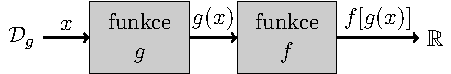
\includegraphics[width=0.45\linewidth]{mai_fig012.pdf}
        \caption{Skládání funkcí \cite[s.~59]{Musilova2009MA1}}
        \label{mai:fig012}
      \end{figure}
      hodnota \(x\) z definičního oboru \(\mathcal{D}_g\) funkce \(g\). Výstupem je číslo \(u = 
      g(x)\), funkční hodnota vnitřní složky v bodě \(x\). Toto číslo smí vstoupit do skříňky 
      představující předpis \(f\), \emph{vnější složku} složené funkce, právě tehdy, je-li prvkem 
      jejího definičního oboru \(\mathcal{D}_f\). V takovém případě najdeme na výstupu ze skříňky 
      \(f\) hodnotu \(y = f(u) = f[g(x)]\). (Jestliže \(g(x)\notin\mathcal{D}_f\), není výstup ze 
      skříňky \(f\) definován.) Vzniká nový předpis \(F\), kterým se některým bodům definičního 
      oboru \(\mathcal{D}_g\), ne všem, ale pouze těm, pro něž \(g(x)\in\mathcal{D}_f\), 
      přiřazují hodnoty \(f[g(x)]\). Definujme nyní složenou funkci přesněji: Předpokládejme, že 
      jsou zadány funkce
      \begin{align*}
        g  &: \mathcal{D}_g\ni x\,\rightarrow\, g(x) = u\in\realset, \\
        f  &: \mathcal{D}_f\ni u\,\rightarrow\, f(u) = y\in\realset. \\
        \shortintertext{označme}
        \mathcal{D} &= \{x|x\in\mathcal{D}_g \text{ a současně } g(x)\in\mathcal{D}_f\}.
      \end{align*}
      Pokud \(\mathcal{D} = \emptyset\), lze definovat funkci
      \begin{equation*}
        F: \mathcal{D}\ni x\rightarrow y = F(x) = f[g(x)]\in\realset, 
           \text{ značíme } F = f \circ g.
      \end{equation*}
      \(F\) se nazývá \emph{složením} neboli \emph{kompozicí} funkcí \(g\) a \(f\). Zápis \(f\circ 
      g\) čteme často také jako \emph{„f po g“}. Skládat lze i větší počet funkcí.

       %-------------------------------------
         % !TeX spellcheck = cs_CZ
\begin{mdframed}[style=mdexam]
  \begin{example}\label{MAI:exam025}
    Uvažme funkci z příkladu \ref{vol02:fyz:fey_exam017}. 
    
    {\centering
    \captionsetup{type=figure}
  %   % !TeX spellcheck = cs_CZ
\documentclass[11pt]{standalone}
\usepackage{xltxtra}
\usepackage[usenames,x11names]{xcolor}
\usepackage{tikz}
\usepackage{pgfplots}
  \pgfplotsset{compat=newest}
\usepackage{amsmath}

\begin{document}
  \begin{tikzpicture}[thick,scale=0.7, every node/.style={transform shape}]
    \begin{axis}[
      xmin = -5, xmax = 5, ymin = -10, ymax = 1.5,
   %   domain = -0.999999:0.999999,
      restrict y to domain=-30:1.5,
      unit vector ratio=1 1 1,  % axis equal
      grid = both,   % both, major
      grid style={line width=.1pt, draw=gray!20},
      major grid style={dashed, line width=.2pt, draw=gray!40},
      minor tick num=4,
      clip = true,
      clip mode=individual,
      axis x line = middle,
      axis y line = middle,
      xlabel={$x$},
    %  xlabel style={at=(current axis.right of origin), anchor=west},
      ylabel={$u,w,y$},
    %  ylabel style={at=(current axis.above origin), anchor=south},
      enlarge y limits={rel=0.13},
      enlarge x limits={rel=0.07},
    ]
    
      \addplot[color=Gold3, samples=1000, smooth, ultra thick, unbounded coords=jump, no markers, 
               domain = -0.999999:0.999999] 
        gnuplot{log10(sqrt(1-x^2))/log10(2)};  
        
     \addplot[color=green, samples=200, smooth, ultra thick, unbounded coords=jump, no markers, 
     domain = -3.3:3.3] 
        gnuplot{1-x^2};
        
     \addplot[color=blue, samples=200, smooth, ultra thick, unbounded coords=jump, no markers, 
     domain = -1:1] 
        gnuplot{sqrt(1-x^2)};  
    \end{axis}
  \end{tikzpicture}
\end{document}
    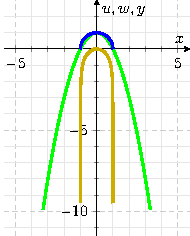
\includegraphics[width=0.6\linewidth]{mai_fig013.pdf}
    \captionof{figure}{K příkladu \ref{MAI:exam025} \(y=\log_2{(\sqrt{1-x^2})}\) 
    \cite[s.~57]{Musilova2009MA1}
    \label{mai:fig013}}
    \par}
    
    Ukážeme, jak tato funkce vzniká postupně složením tří funkcí a jak při tom dochází k postupnému 
    omezování definičního oboru. Písmeny \(\mathcal{D}\) a \(H\) s příslušným indexem budeme značit 
    definiční obory a obory hodnot jednotlivých funkcí.
    \begin{gather*}
      \begin{align*}
        g&:  \realset =\mathcal{D}_g\ni x\rightarrow u=g(x) = 1- x^2  \in\mathcal{H}_g=(-\infty,1], \\
        h&: [0,\infty)=\mathcal{D}_h\ni u\rightarrow w=h(u) = \sqrt{u}\in\mathcal{H}_h=[0,\infty),  \\
       \shortintertext{\(\mathcal{D}_h\cap\mathcal{H}_g = [0,1]\Rightarrow\mathcal{D}_{h\circ g}=[-1,1], 
                       \mathcal{H}_{h\circ g} = [0,1],\)}                                    \\
       f&:(0,\infty)=\mathcal{D}_f\ni w \rightarrow y=f(w)=\log_2w\in\mathcal{H}_f=\realset  \\
       \shortintertext{\(\mathcal{H}_{h\circ g}\cap\mathcal{D}_f = (0,1] 
                       \Rightarrow\mathcal{D}_F=(-1,1),\mathcal{H}_F=(-\infty,0].\)} 
      \end{align*}
    \end{gather*}
    Je tedy
    \begin{gather*}
      \begin{align*}
        F:\mathcal{D}_F\ni x\rightarrow 
        y&=F(x)=(f\circ(h\circ g))(x) = f{h[g(x)]}          \\
        &= \log_2\sqrt{1-x^2}\in(-\infty,0].
      \end{align*}
    \end{gather*}
    Názorněji než tento zápis ukazuje situaci obrázek \ref{mai:fig013}.
  \end{example}
\end{mdframed}
       %-------------------------------------
      
      Může vzniknout otázka, jak rozpoznáme vnitřní a vnější složku složené funkce. Rozlišit 
      vnitřní a vnější složku třeba u funkcí \(\cos(x^2)\) a \((cos x)^2\) není problém. Hned také 
      vidíme, že obecně \(f\circ g\neq g\circ f\), i když by definiční obory funkcí na pravé i levé 
      straně měly neprázdný průnik. Jsou však i případy na první pohled méně zřetelné, jak ukazuje 
      následující příklad.
      
      %-------------------------------------
        % !TeX spellcheck = cs_CZ
\begin{mdframed}[style=mdexam]
  \begin{example}\label{mai:exam026}
    (Určení vnitřní a vnější složky) Uveďme příklad dvou funkcí \(F(x)=\sqrt{x^2}\) a \(G(x) =
    (\sqrt{x})^2\). Liší se tyto funkce, nebo jde o tutéž funkci, jen jinak zapsanou? Vidíme, že
    platí

    \begin{align*}
      \mathcal{D}_F &=\realset, F(x)=\abs{x}\forall x\in\mathcal{D}_F, \mathcal{H}_F = [0, infty),\\
      \mathcal{D}_G &=[0, \infty), G(x)=x\forall    x\in\mathcal{D}_G, \mathcal{H}_G = [0, infty).
    \end{align*}
    Funkce \(F\) a \(G\) mají různé definiční obory, ale na jejich průniku dávají stejné funkční
    hodnoty. Ani zde však obecně nelze pořadí skládání funkcí zaměňovat.
  \end{example}
\end{mdframed}
      %-------------------------------------
       
      Funkce \(F\) a \(G\) mají různé definiční obory, ale na jejich průniku dávají stejné funkční 
      hodnoty. Ani zde však obecně nelze pořadí skládání funkcí zaměňovat.
      
      Nyní se pusťme do vybudování pojmu inverzní funkce k funkci \(f\). Představme si, že funkční
      hodnota \(y = f(x)\) zadané funkce
      \begin{equation*}
        f: \mathcal{D}_f\ni x \rightarrow f(x)\in\mathcal{H}_f
      \end{equation*}
      představuje „zakódovanou“ informaci o hodnotě \(x\). Položme si otázku, zda a za jakých 
      podmínek dokážeme sestavit „černou skříňku“, na jejímž výstupu by se při vstupu obrazu \(y = 
      f(x)\) objevila hodnota \(x\). Omezení takové možnosti je názorně vidět na obrázku 
      \ref{mai:fig014}. V případě funkce \(f(x)\) lze ke všem obrazům \(y \in \mathcal{H}_f\) najít 
      vzory, v případě funkce \(g(x)\) to možné není, neboť jeden a týž obraz lze získat z několika 
      vzorů. Pro který bychom se tedy měli rozhodnout?
      
      \begin{figure}[ht!] %\ref{mai:fig014}
        \centering
%        % !TeX spellcheck = cs_CZ
% Skládání funkcí \cite[s.~61]{Musilova2009MA1}

\documentclass[11pt]{standalone}
\usepackage{xltxtra}
\usepackage[usenames,x11names]{xcolor}
\usepackage{tikz}
\usepackage{pgfplots}
  \pgfplotsset{compat=newest}
\usepackage{amsmath}
\usepackage{amsfonts}       % \mathbb{R}
  \newcommand{\realset}{\mathbb{R}}

\begin{document}
  \begin{tikzpicture}[fill=black!20]
  %  \draw[help lines] (-1,-2) grid (6,3);
    \path (0,0) node(a) [ ] {\(\mathcal{D}_f\)}
    (2,0) node(b) [rectangle,rotate=0,draw,fill] 
      {\(\begin{array}{c} \text{funkce} \\ f  \end{array}\)}
    (4.5,0) node(c) [rectangle,rotate=0,draw,fill] 
      {\(\begin{array}{c} \text{funkce} \\ f^{-1}  \end{array}\)}
    (7,0) node(d) [ ] {\(\realset\)};
    \draw[thick,->] (a.east) -- (b);
    \draw[thick,->] (b.east) -- (c);
    \draw[thick,->] (c.east) -- (d);
    \path [ ] (a.east) -- (b.west)   node [above,midway] {\(x\)};
    \path [ ] (b.east) -- (c.west)   node [above,midway] {\(f(x)\)};
    \path [ ] (c.east) -- (d.west)   node [above,midway] {\(x\)};
  \end{tikzpicture}
\end{document}
        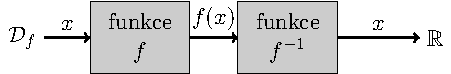
\includegraphics[width=0.45\linewidth]{mai_fig014.pdf}
        \caption{Skládání funkcí \cite[s.~61]{Musilova2009MA1}}
        \label{mai:fig014}
      \end{figure}
       Aby bylo možné vzor zpětně identifikovat na základě znalosti obrazu, je třeba, aby funkce 
       \(f\) byla \emph{prostá}, tj. aby předpis \(f\) přiřazoval každým dvěma různým vzorům \(X_1 
       \neq x_2\) dva různé obrazy \(f(x_1) \neq f(x_2)\). Často lze tohoto požadavku docílit tím, 
       že se místo funkce \(f\) s definičním oborem \(\mathcal{D}_f\) spokojíme s funkcí, která 
       vznikne omezením \emph{(restrikcí)} té původní na „menší“ definiční obor, zato však již bude 
       prostá. U funkce \(g\) na obrázku \ref{mai:fig016} by tak stačilo omezit definiční obor 
       například na množinu \(\mathcal{D}_g\). Než inverzní funkci definujeme, ukažme si způsob 
       jejího nalezení na známém příkladu.

       \begin{figure}[ht!]
         \centering  
         \begin{tabular}{cc}
           \subfloat[ ]{\label{mai:fig016a}
             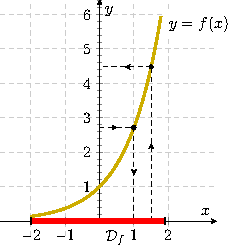
\includegraphics[width=0.45\linewidth]{mai_fig016a.pdf}}              &
           \subfloat[ ]{\label{mai:fig016b}
             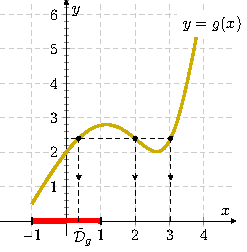
\includegraphics[width=0.45\linewidth]{mai_fig016b.pdf}}              \\
         \end{tabular}
         \caption{K pojmu inverzní funkce}
         \label{mai:fig016}
       \end{figure}
      
      %-------------------------------------
        % !TeX spellcheck = cs_CZ
\begin{mdframed}[style=mdexam]
  \begin{example}\label{MAI:exam027}
    (Nalezení inverzní funkce): Funkci 
    \begin{equation*}
      y = \log_2(\sqrt{1-x^2})
    \end{equation*}
    Jsme již z různých hledisek rozebrali v příkladech \ref{vol02:fyz:fey_exam017} a
    \ref{MAI:exam025}. Hodí se i nyní.

    {\centering
    \captionsetup{type=figure}
  %  % !TeX spellcheck = cs_CZ
% K příkladu \ref{mai:exam027} \(y=\log_2{(\sqrt{1-x^2})}

\documentclass[11pt]{standalone}
\usepackage{xltxtra}
\usepackage[usenames,x11names]{xcolor}
\usepackage{tikz}
\usepackage{pgfplots}
  \pgfplotsset{compat=newest}
\usepackage{amsmath}

\begin{document}
  \begin{tikzpicture}[thick,scale=0.7, every node/.style={transform shape}]
    \begin{axis}[
      xmin = -5, xmax = 5, ymin = -5, ymax = 1.5,
   %   domain = -0.999999:0.999999,
      restrict y to domain=-30:1.5,
      unit vector ratio=1 1 1,  % axis equal
      grid = both,   % both, major
      grid style={line width=.1pt, draw=gray!20},
      major grid style={dashed, line width=.2pt, draw=gray!40},
      minor tick num=4,
      clip = true,
      clip mode=individual,
      axis x line = middle,
      axis y line = middle,
      xlabel={\(x\)},
    %  xlabel style={at=(current axis.right of origin), anchor=west},
      ylabel={\(y\)},
    %  ylabel style={at=(current axis.above origin), anchor=south},
      enlarge y limits={rel=0.13},
      enlarge x limits={rel=0.07},
    ]
    
      \addplot[color=Gold3, samples=1000, smooth, ultra thick, unbounded coords=jump, no markers, 
               domain = 0:0.9995] 
        gnuplot{log10(sqrt(1-x^2))/log10(2)};  
        
      \addplot[color=blue, samples=200, smooth, ultra thick, unbounded coords=jump, no markers, 
               domain = -5:0] 
        gnuplot{sqrt(1-2^(2*x))};  
    \end{axis}
  \end{tikzpicture}
\end{document}
    \luafigure[0.9]{mai_fig015.pdf}
    \captionof{figure}{K příkladu \ref{MAI:exam027} \(y=\log_2{(\sqrt{1-x^2})}\) 
    \cite[s.~62]{Musilova2009MA1}
    \label{mai:fig015}}
    \par}
    
    Na obrázku \ref{mai:fig013} máme dokonce její graf, a tak vidíme, že \textbf{není} na svém 
    definičním oboru \((-1, 1)\) \textbf{prostá}. Omezme proto její definiční obor na interval 
    \(\mathcal{D} = [0, 1)\), na němž již prostá je (část grafu vpravo od osy \(y\)). Pro danou 
    hodnotu obrazu \(y \in (-\infty,0]\) můžeme již jednoznačně určit hodnotu \(x\) jednoduchou 
    úpravou:
    \begin{align*}
      y = \log_2(\sqrt{1-x^2}) &\Rightarrow \sqrt{1-x^2} = 2^y   \\
                               &\Rightarrow x^2 = 1 - 2^{2y}     \\
                               &\Rightarrow x = \sqrt{1 - 2^{2y}}
    \end{align*}
    Formální záměnou \(x \leftrightarrow y\) dostáváme inverzní funkci k funkci \(f\),
    \begin{equation*}
      y =f^{-1}(x) = \sqrt{1 - 2^{2x}}.
    \end{equation*}
    Grafy obou funkcí jsou na obrázku \ref{mai:fig015}.
  \end{example}
\end{mdframed}
      %-------------------------------------
      
      Ze způsobu konstrukce funkce \(f^{-1}\) v předchozím příkladu je vidět, že 
      \(\mathcal{D}_{f^{-1}} = \mathcal{H}_f\), \(\mathcal{H}_{f^{-1}} = \mathcal{D}_f\) a graf 
      inverzní funkce je obrazem grafu prosté funkce \(f\) při osové symetrii v rovině 
      souřadnicových os vzhledem k ose prvního a třetího kvadrantu. Nyní již definujeme inverzní 
      funkci obecně. Předpokládejme, že funkce \(f : \mathcal{D}_f\ni x \rightarrow y = f(x)\ni 
      \mathcal{H}_f\) je prostá na svém definičním oboru. Pak existuje funkce \(f^{-1}\) definovaná 
      jako
      \begin{equation}\label{mai:eq029}
        f^{-1} :\mathcal{H}_f\ni x\rightarrow y = f^{-1}(x)\in\mathcal{D}_f\Leftrightarrow x = f(y).
      \end{equation}
      Funkci \(f^{-1}\) nazýváme \textbf{inverzní funkcí k funkci} \(f\). Ještě shrneme pravidla 
      pro skládání funkcí a pro inverzní funkce:

      \begin{itemize}\addtolength{\itemsep}{-0.5\baselineskip}
        \item asociativní zákon pro skládání funkcí
          \begin{equation}\label{mai:eq030}
            f(x)\circ(h(x)\circ g(x)) = f(x)\circ h(x) \circ g(x)
          \end{equation}
        \item distributivní zákon zleva 
          \begin{equation}\label{mai:eq031}
            f(x) \circ (h(x) + g(x)) = f(x) \circ h(x) + f(x) \circ g(x)
          \end{equation}
        \item existence univerzálního neutrálního  prvku \(O\) (nulová funkce \(O:\mathcal{D}\ni x 
          \rightarrow O(x)=0\))
          \begin{equation}\label{mai:eq032}
            f(x) + O = O + f(x) = f(x)
          \end{equation}
        \item existence právě jednoho opačného prvku k funkci \(f\), přičemž \((-f)(x) = -f(x)\)
          \begin{equation}\label{mai:eq033}
            f(x)+(-f(x))=(-f(x))+f(x)=O
          \end{equation}
        \item komutativní zákon pro součet funkcí
          \begin{equation}\label{mai:eq034}
            f(x) + g(x) = g(x) + f(x)
          \end{equation}
        \item asociativní zákon pro součet funkcí  
          \begin{equation}\label{mai:eq035}
            (f(x) + g(x)+h(x) = f(x) + (g(x) + h(x)
          \end{equation}
        \item existence univerzálního neutrálního  prvku \(O\) (nulová funkce \(O:\mathcal{D}\ni x 
          \rightarrow O(x)=0\))
          \begin{equation}\label{mai:eq036}
            f(x) + O = O + f(x) = f(x)
          \end{equation}        
      \end{itemize}   
      Předchozí vztahy platí na patřičně zúžených definičních oborech funkcí, které do nich 
      vstupují.
      
  %-------------------------------------------------------------------------------------------------
  \section{Elementární funkce}
      Základními elementárními funkcemi nazýváme \cite[s.~10]{PolakMA1}:
%      \begin{displaymath}
%        \xymatrix{
%        \mbox{mocninné} & *+[F]{\mbox{Elementární 
%        funkce}}\ar@{->}[l]\ar@{->}[dl]\ar@{->}[d]\ar@{->}[dr]\ar@{->}[r]&\mbox{exponenciální} \\
%        \mbox{goniometrické}       &   \mbox{logaritmické}      & \mbox{cyklometrické}
%        }
%      \end{displaymath}
    %------------- Goniometrické funkce ------------------------------------------------------------
    \subsection{Goniometrické funkce}  
    \begin{itemize}
      \item \textbf{Základní vzorce pro goniometrické funkce}
        \begin{align}
          \sin^2\alpha     &+ \cos^2\alpha = 1      &\forall\alpha\in\realset \label{MA1:eq_sincos} \\ 
          \abs{\sin\alpha} &= \sqrt{1-\cos^2\alpha} &\forall\alpha\in\realset \label{MA1:eq_sinabs} \\ 
          \abs{\cos\alpha} &= \sqrt{1-\sin^2\alpha} &\forall\alpha\in\realset \label{MA1:eq_cosabs}
        \end{align}  
      \item \textbf{Součtové vzorce}
        \begin{align}
        % \nonumber to remove numbering (before each equation)
          \sin(\alpha + \beta) 
            &= \sin\alpha\cdot\cos\beta 
             - \sin\beta\cdot\cos\alpha           \label{MA1:eq_sinxpy}  \\ 
          \sin(\alpha - \beta) 
            &= \sin\alpha\cdot\cos\beta 
             + \sin\beta\cdot\cos\alpha           \label{MA1:eq_sinxmy}  \\ 
          \cos(\alpha + \beta) 
            &= \cos\alpha\cdot\cos\beta 
             - \sin\alpha\cdot\sin\beta           \label{MA1:eq_cosxpy}  \\ 
          \cos(\alpha - \beta) 
            &= \cos\alpha\cdot\cos\beta 
             + \sin\alpha\cdot\sin\beta           \label{MA1:eq_cosxmy}  \\ 
          \tan(\alpha\pm\beta) 
            &= \frac{\tan\alpha\pm\tan\beta}{1\mp\tan\alpha\cdot\tan\beta} \label{MA1:eq_tanxpmy}\\ 
          \cot(\alpha\pm\beta) 
            &= \frac{1\mp\cot\alpha\cdot\cot\beta}{\cot\alpha\pm \cot\beta} \label{MA1:eq_cotxpmy}
        \end{align}
        Součtové vzorce lze odvodit několika způsoby; jednoduchý způsob důkazu
        lze provést pomocí skalárního součinu vektorů.
      \item \textbf{Vzorce pro dvojnásobný úhel $2\alpha$}
        \newline Pro každé $\alpha\in R$ platí:
        \begin{align}
          \sin(2\alpha)   &= 2\sin\alpha\cos\alpha                \label{MA1:eq_sin2x} \\ 
          \cos(2\alpha)   &= \cos^2\alpha - \sin^2\alpha          \label{MA1:eq_cos2x} \\ 
          \tan(2\alpha)   &= \frac{2\tan\alpha}{1-\tan^2\alpha}   \label{MA1:eq_tan2x} \\ 
          \cot(2\alpha)   &= \frac{\cot^2\alpha - 1}{2\cot\alpha} \label{MA1:eq_cot2x}
        \end{align}
      \item \textbf{Vzorce pro poloviční úhel $\displaystyle\frac{\alpha}{2}$}
        \begin{align}
          \left\lvert\sin\frac{\alpha}{2}\right\rvert   
            &= \sqrt{\frac{1-\cos\alpha}{2}}                      \label{MA1:eq_sinx2} \\ 
          \left\lvert\cos\frac{\alpha}{2}\right\rvert   
            &= \sqrt{\frac{1+\cos\alpha}{2}}                      \label{MA1:eq_cosx2} \\ 
          \left\lvert\tan\frac{\alpha}{2}\right\rvert   
            &= \sqrt{\frac{1-\cos\alpha}{1+\cos\alpha}}           \label{MA1:eq_tanx2} \\ 
          \left\lvert\cot\frac{\alpha}{2}\right\rvert   
            &= \sqrt{\frac{1+\cos\alpha}{1-\cos\alpha}}           \label{MA1:eq_cotx2}
        \end{align}
    \end{itemize}
    Vzorce \ref{MA1:eq_sinx2} a \ref{MA1:eq_cosx2} odvodíme pomocí vzorců \ref{MA1:eq_cos2x} a \ref{MA1:eq_sincos}:
    \begin{align*}
      \cos\alpha &= 
      \cos2\frac{\alpha}{2}=\cos^2\frac{\alpha}{2}-\sin^2\frac{\alpha}{2}=1-2\sin^2\frac{\alpha}{2} \\
      \sin^2\frac{\alpha}{2} &= \frac{1-\cos\alpha}{2}   \\
      \cos^2\frac{\alpha}{2} &= 1 - \sin^2\frac{\alpha}{2} = \frac{1+\cos\alpha}{2} 
    \end{align*}
    a dále užijeme vztahu $\sqrt{a^2}=\abs{a}$ (platí pro každé $a\in\realset$). Užitím součtových vzorců a toho že, 
	$\sin\frac{\pi}{2} = 1$, $\cos\frac{\pi}{2} = 0$, $\sin\pi = 0$ a $\cos\pi = -1$ lze snadno odvodit, 
	že pro každé $\alpha\in R$ platí
    \begin{align*}
      \sin\left(\frac{\pi}{2}+\alpha\right) &=  \cos\alpha  &   \cos\left(\frac{\pi}{2}+\alpha\right) &= -\sin\alpha \\
      \sin\left(\frac{\pi}{2}-\alpha\right) &=  \cos\alpha  &   \cos\left(\frac{\pi}{2}-\alpha\right) &=  \sin\alpha \\
      \sin\left(\pi+\alpha\right)           &= -\sin\alpha  &   \cos\left(\pi+\alpha\right)           &= -\cos\alpha \\
      \sin\left(\pi-\alpha\right)           &=  \sin\alpha  &   \cos\left(\pi-\alpha\right)           &= -\cos\alpha \\
    \end{align*}
    \newline Důkaz provedeme pro první z těchto často užitečných vzorců (u ostatních je odvození obdobné):
    $$\sin\left(\frac{\pi}{2}+\alpha\right) = \sin\frac{\pi}{2}\cos\alpha + \cos\frac{\pi}{2}\sin\alpha = 1\cdot\cos\alpha + 0\cdot\sin\alpha.$$
 
    %-----------------------------------------------------------------------------------------------
    \subsection{Zobrazení v jiných strukturách}
    %-----------------------------------------------------------------------------------------------
    \subsection{Cvičení}
  %================ Podkapitola: Limita funkce =====================================================
  \section{Limity všeho druhu}  
    „Limes“ znamená latinsky příční cesta, mez, v přeneseném významu pak hranice, pomezí, atd. V 
    matematice představuje limita hodnotu, ke které se „neomezeně blíží hodnota funkce, jestliže se 
    hodnota proměnné neomezeně blíží zadanému číslu“. Poslední formulace musí být v uvozovkách, 
    protože je i přes svou dobrou názornost velice nepřesná. A takové nepřesnosti nejsou v 
    matematice dovoleny. K čemu vůbec úvaha o limitě je? Stačí přece do funkčního předpisu hodnotu 
    proměnné dosadit a získat funkční hodnotu. Tak jednoduché to ale není. Funkční hodnota pro 
    danou hodnotu proměnné \(x\) vůbec nemusí být definována, zato může být definována pro hodnoty 
    velmi blízké. Nebo definována je, ale pro hodnoty proměnné, které jsou k \(x\) velmi blízké, 
    jsou funkční hodnoty od \(f(x)\) velmi vzdálené. Potřebnost pojmu limita ukážeme na 
    geometrickém a fyzikálním příkladu.
    
    V matematické analýze hraje např. důležitou úlohu podíl \cite[s.~117]{Brabec1989}
    \begin{equation*}
      \dfrac{\varphi(x) - \varphi(a)}{x - a}
    \end{equation*}
    kde \(\varphi\) je daná funkce, \(a\) pevný bod. Tento podíl tzv. \emph{přírůstku funkce} 
    \(\varphi(x) — \varphi(a)\) k přírůstku argumentu \(x — a\) může značit např. \emph{průměrnou 
    rychlost pohybu bodu po přímce}, jehož zákon dráhy je dán vztahem \(y = \varphi(x)\), kde \(y\) 
    je dráha, kterou bod urazí za čas \(x\). Zajímá nás, jak se mění hodnota tohoto podílu — jinak 
    řečeno, jak se mění hodnota funkce \(f\) dané vztahem
    \begin{equation}\label{mai:eq037}
      f(x) = \dfrac{\varphi(x) - \varphi(a)}{x - a}
    \end{equation}
    když hodnoty argumentu \(x\) se blíží k číslu \(a\), což často značíme \(x\rightarrow a\). V 
    uvedeném fyzikálním významu daného podílu se ptáme, jak se mění průměrná rychlost pohybu, když 
    se časový úsek zkracuje. Je zřejmé, že musí být stále \(x \neq a\) a že jmenovatel se blíží k 
    nule; obvykle se blíží k nule i čitatel. Jakých hodnot však nabývá přitom podíl, tj. jaké jsou 
    hodnoty funkce \(f(x)\)? Než vyslovíme přesnou definici limity, uvedeme ještě pár jednoduchých 
    příkladů.

    %-------------------------------------
      % !TeX spellcheck = cs_CZ
\wikitextrule
\begin{example}\label{MAI:exam028}
  Nechť \(\varphi(x) = x^2\), \(a = 1\). Potom \(f(x) = (x^2 — 1 )/(x — 1)\). Pro \(x \neq 1\) je 
  hodnota funkce \(f\) rovna \(f(x) = (x + 1) (x - 1 )/(x - 1) = x + 1\). Když \(x \rightarrow 1\) 
  (přičemž stále \(x \neq 1\)), pak \(f(x) \rightarrow 2\) (viz obr. 51). Zároveň je také patrný 
  charakter tohoto blížení: Hodnoty \(f(x)\) jsou libovolně blízko číslu \(2\), jestliže hodnoty 
  proměnné \(x\) jsou dostatečně blízké číslu \(1\). To můžeme říci také takto: 
  
  {\centering
   \captionsetup{type=figure}
%   % !TeX spellcheck = cs_CZ

\documentclass[11pt]{standalone}
\usepackage{xltxtra}
\usepackage[usenames,x11names]{xcolor}
\usepackage{tikz}
  \usetikzlibrary{intersections}
  \usetikzlibrary{decorations.markings}
\usepackage{pgfplots}
  \pgfplotsset{compat=newest}
\usepackage{amsmath}


\begin{document}
  \begin{tikzpicture}[thick,scale=0.7, 
      every node/.style={transform shape},
      ]
  
  \tikzset{->-/.style={decoration={
    markings,
    mark=at position #1 with {\arrow{stealth}}},postaction={decorate}}}
    
    \begin{axis}[
      xmin = -1.5, xmax = 2.5, ymin = 0, ymax = 3.5,  % osy
      domain = -1:3.5,
      restrict y to domain=0:3,
      axis equal image,
      grid = major,   % both
      grid style={line width=.1pt, draw=gray!20},
      major grid style={dashed, line width=.2pt, draw=gray!40},
      clip = true,
      clip mode=individual,
      xtick={-2,-1,1,2,3,4}, % make steps of length 0.2
      ytick={0,1,2,3,4,5}, 
      axis x line = middle,
      axis y line = middle,
      xlabel={$x$}, ylabel={$y$},
      enlarge y limits={rel=0.07},
      enlarge x limits={rel=0.07}
      ]
      
      \addplot[color=Gold3, samples=10, smooth, ultra thick, unbounded coords=jump, no markers, 
               domain = -1:2.2] 
        gnuplot{x+1}; 
      
      \node [fill=white] at (rel axis cs: 0.9,0.9) {\(y=\dfrac{x^2-1}{x-1}\)};
      
      \draw[line width = 3pt, red, line cap=butt] (0.5,0) -- (1.5,0);
      \draw [thick] (0.5,-.2) node[below] {\(1-\delta\)} -- (0.5,0.1);
      \draw [thick] (1.5,-.2) node[below] {\(1+\delta\)} -- (1.5,0.1);
      
      \draw[line width = 3pt, red, line cap=butt] (0,1.5) -- (0,2.5);
      \draw [thick] (-.2, 1.5) node[left] {\(1-\varepsilon\)} -- (0.1, 1.5);
      \draw [thick] (-.2, 2.5) node[left] {\(1+\varepsilon\)} -- (0.1, 2.5 );
      
      \draw[dashed] (0.5,0) -- (0.5,1.5) -- (0,1.5);
      \draw[dashed] (1.5,0) -- (1.5,2.5) -- (0,2.5);
      \draw[dashed] (1,0) -- (1,2) -- (0,2);
  
      \draw[->-=.5] (1.25,0) node[below] {\(x\)} -- (1.25,2.25);
      \draw[->-=.5] (1.25,2.25) -- (0,2.25) node[left] {\(f(x)\)}; 
       
      \draw[black,fill=white] (1,0) circle (.4ex);
      \draw[black,fill=white] (1,2) circle (.4ex);
      \draw[black,fill=white] (0,2) circle (.4ex);
    \end{axis}
  \end{tikzpicture}
\end{document}
    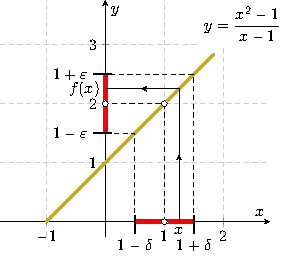
\includegraphics[width=0.45\linewidth]{mai_fig017.pdf}
   \captionof{figure}{K příkladu \ref{MAI:exam028}
   \cite[s.~118]{Brabec1989}
   \label{mai:fig017}}
  \par}
  
  Zvolíme-li libovolně malé okolí bodu \(2\), pak vždy lze najít okolí bodu \(1\) takové, že pro 
  každé \(x \neq 1\) z tohoto okolí bude ležet hodnota \(f(x)\) ve zvoleném okolí čísla \(2\). 
  Ještě jinak formulováno: K libovolně malému \(\varepsilon > 0\) existuje \(\delta > 0\) tak, 
  že pro každé \(x\), pro něž \(0 < \abs{x — 1} \ll \delta\), platí \(\abs{f(x) — 2} < 
  \varepsilon\) (viz obr. \ref{mai:fig017}). O funkci \(f\) s touto vlastností říkáme, že má v bodě 
  \(1\) limitu \(2\) a píšeme symbolicky \(lim_{x \to 1}f(x) = 2\) nebo \(f(x) \rightarrow 2\) pro 
  \(x \rightarrow 1\).
\end{example}
















    %-------------------------------------

    Definičním oborem funkce z příkladu \ref{MAI:exam028} je tedy množina \(\mathcal{D} = \realset 
    — {1}\) (pro \(a = 1\) by ve jmenovateli zlomku byla nula). Grafem funkce je tedy přímka s 
    „vynechaným“ bodem \([1, 2]\) (obr. \ref{mai:fig017}). V bodě \(a = 1\) funkční hodnota není 
    definována. Pokud bychom chtěli rozšířit definiční obor funkce na celou reálnou osu, musíme 
    předepsat, jaké hodnoty má funkce nabývat v bodě \(a = 1\). Původní vzorec, jímž je funkce 
    zadána, výpočet hodnoty \(f(1)\) neumožňuje. Dodatečné zadání funkční hodnoty, její 
    \emph{dodefinování}, můžeme provést zcela libovolně. Zvolme například \(f(1) = 2\). Jiná 
    možnost, jak funkci dodefinovat, je například \(f(1) =-1\). Které číslo je ovšem limitou funkce 
    \(f(x)\) v bodě \(a = 1\)? Je to číslo \(2\), které je v případe \(f(x) = x+1\) její funkční 
    hodnotou? Nebo číslo \(-1\)? A nebo nějaká jiná hodnota? Intuice nám napovídá, že je to číslo 
    \(2\). Když dvojku použijeme pro dodefinování funkce, přetržený graf se „zacelí“. Vidíme, že 
    vezmeme-li dostatečně malý interval proměnné \(x\) v blízkosti bodu \(a=1\) můžeme docílit 
    toho, že všechny odpovídající funkční hodnoty \(f(x)\) budou ležet tak blízko hodnotě \(2\), 
    jak si předem určíme. Skutečně, zkusme docílit toho, aby hodnoty \(f(x)\) ležely v intervalu 
    \((\num{1.99}, \num{2.01})\), tj.
    \begin{equation*}
      \num{1.99} < x + 1 < \num{2.01} \Rightarrow \num{0.99} < x < \num{1.01},\qquad x\neq1.
    \end{equation*}
    Podařilo se. A kdybychom interval \(I(\varepsilon) = (2 - \varepsilon, 2 + \varepsilon)\) 
    funkčních hodnot kolem \(2\) ještě zmenšili, podařilo by se opět najít (o něco menší) interval 
    kolem bodu \(a = 1\) tak, aby pro všechny hodnoty \(x\) v něm (samozřejmě s případnou výjimkou 
    hodnoty \(a =2\)) platilo \(f(x)\in I(\varepsilon)\). A takto bychom mohli \(\varepsilon\) 
    stále zmenšovat. Jak by takový postup dopadl s hodnotou \(-1\), která, jak intuitivně cítíme, 
    limitou funkce v bodě \(a = 1\) není, protože je graf funkce od bodu \([-1,0]\) dost vzdálen? 
    Vezměme třeba interval (\num{-0.5}, \num{0.5}) a hledejme hodnoty \(x\) obdobně jako v 
    předchozím případě. Požadujeme
    \begin{equation*}
      \num{-0.5} < x + 1 < \num{0.5} \Rightarrow \num{-1.5} < x < \num{-0.5}.
    \end{equation*}
    Tento interval vůbec neobsahuje bod \(a = 1\). Dostali jsme se mimo blízkost bodu \(a = 1\).

    %-------------------------------------
      % !TeX spellcheck = cs_CZ
\begin{mathexam}{Najdi limitu funkce \(\varphi(x) = \sqrt[3]{x}\) v bodě \(a = 0\) pomocí
  \eqref{mai:eq037}}{exam029} 
   
  Nechť \(\varphi(x) = \sqrt[3]{x}\), \(a = 0\). Pak \[f(x) = \dfrac{\sqrt[3]{x}}{x}\]. Pro \(x \neq
  0\) je \[f(x) = \frac{1}{\sqrt[3]{x^2}}\]. Jestliže \(x \to 0\), pak hodnoty \(f(x)\) neomezeně
  vzrůstají, protože jmenovatel zlomku se blíží kladnými hodnotami k nule a čitatel je stále roven
  \(1\) (viz obr. \ref{mai:fig018}). Místo rčení \emph{„funkce neomezeně roste“} pro \(x \to 0\)
  říkáme též ]\emph{„funkce se blíží k \(+\infty\)“} pro \(x \to 0\) a píšeme 
  \begin{equation*}
    \lim\limits_{x\to 0} f(x) = +\infty \text{ nebo } f(x)\to +\infty\text{ pro } x\to0.
  \end{equation*}
  Říkáme, že limita funkce \(f\) v bodě \(0\) je rovna \(+\infty\). 
    
  {\centering
  \captionsetup{type=figure}
%   \documentclass[11pt]{standalone}
\usepackage{xltxtra}
\usepackage[usenames,x11names]{xcolor}
\usepackage{tikz}
  \usetikzlibrary{intersections}
  \usetikzlibrary{decorations.markings}
\usepackage{pgfplots}
  \pgfplotsset{compat=newest}
  
\usepackage{amsmath}

\begin{document}
  \begin{tikzpicture}[thick,scale=0.7, 
      every node/.style={transform shape},
      ]
  
  \tikzset{->-/.style={decoration={
    markings,
    mark=at position #1 with {\arrow{stealth}}},postaction={decorate}}}
    
    \begin{axis}[
      xmin = -2.5, xmax = 2.5, ymin = 0, ymax = 3.5,  % osy
      domain = -1:3.5,
      restrict y to domain=0:3.4,
      axis equal image,
      grid = major,   % both
      grid style={line width=.1pt, draw=gray!20},
      major grid style={dashed, line width=.2pt, draw=gray!40},
      clip = true,
      clip mode=individual,
      xtick={-2,-1,1,2,3,4}, % make steps of length 0.2
      ytick={0,1,2,3,4,5}, 
      axis x line = middle,
      axis y line = middle,
      xlabel={\(x\)}, ylabel={\(y\)},
      enlarge y limits={rel=0.07},
      enlarge x limits={rel=0.07},
      ]
  
        \addplot[color=Gold3, samples=100, smooth, ultra thick, unbounded coords=jump,
                 no markers, domain = 0.1:2, name path global=func1] 
           gnuplot{1/((x^2.0)^(1/3.0))};
  
        \addplot[color=Gold3, samples=100, smooth, ultra thick, unbounded coords=jump,
                 no markers, domain = -2:-0.1, name path global=func2] 
           gnuplot{real(1/((x^2.0)^(1/3.0)))};
  
        \node [fill=white] at (rel axis cs: 0.75,0.5) {\(y=\dfrac{1}{\sqrt[3]{x^2}}\)};
  
        \path[name path=line] (-1,1.5) -- (1,1.5); 
            % Intersections points
            \path [name intersections={of=func1 and line,by={P1}}] (P1) node [] {};
  
        \path[name path=line] (-1,1.5) -- (1,1.5); 
            % Intersections points
            \path [name intersections={of=func2 and line,by={Q1}}] (Q1) node [] {};
        
        \draw[black,fill=black] (P1) circle (.3ex);
        \draw[black,fill=black] (Q1) circle (.3ex);
        \path (P1 |- 3,0) -- (P1) -- (P1 -| 0,3) node (X) {};
  
        \draw[thick,red, fill=white] ([shift=(0:1mm)]X) arc (0:180:1mm);
        \draw[->-=.5, dashed]  (P1 |- 3,-0.1)  
          node[below] {\(\delta\)} -- (P1) -- (P1 -| 0,3);
        \draw[->-=.5, dashed]  (Q1 |- -3,-0.1) 
          node[below] {\(\delta\)} -- (Q1) -- (Q1 -| 0,3);
  
        \draw[line width = 2pt, red, line cap=butt] (Q1 |- 3,0) -- (P1 |- 3,0);
        
        \path[name path=line] (-0.7,2.5) -- (0.7,2.5); 
            % Intersections points
            \path [name intersections={of=func1 and line,by={P1}}] (P1) node [] {};
            \draw[->-=.4, dashed, thin,gray] (P1 |- 3,-0.05) node[below] {\(x\)} -- (P1);
            \draw[->-=1, thin, gray] (P1) -- (P1 -| 0,3) node[left, fill=white] {\(f(x)\)};
        \draw[thick,red] (X) node[below left] {\(q\)} -- ++(0cm,2.5cm);
  
       \draw[black,fill=white] (0,0) node[below left] {\(O\)} circle (.4ex);
    \end{axis}
  \end{tikzpicture}
\end{document}
  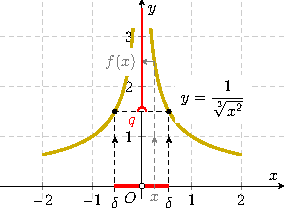
\includegraphics[width=0.8\linewidth]{mai_fig018.pdf}
  \captionof{figure}{K příkladu \ref{MAI:exam029}
  \cite[s.~118]{Brabec1989}
  \label{mai:fig018}}
  \par}
  
  Přesně to znamená toto: Zvolíme-li libovolně velké \(q > 0\), můžeme nalézt \(\delta > 0\) tak, že
  pro každé \(x \neq 0\), pro něž \(\abs{x} < \delta\), platí \(f(x) > q\). 
  
  To lze říci i takto: Zvolíme-li libovolně okolí bodu \(+\infty\), existuje okolí bodu \(0\) tak,
  že pro každé \(x \neq 0\) z tohoto okolí je \(f(x)\) ve zvoleném okolí \(+\infty\) (viz obr.
  \ref{mai:fig018}).
\end{mathexam}
















    %-------------------------------------

    Je třeba říci, že při zkoumání limit funkcí nás nezajímají jen funkce „tvaru“ 
    (\ref{mai:eq037}), i když tento případ je v diferenciálním počtu velmi častý, jak poznáme v 
    kap. \ref{mai:IchapIV}. Někdy nás zajímá i chování funkcí v okolí nevlastních bodů \(-\infty\), 
    \(+\infty\) 

    %-------------------------------------
      % !TeX spellcheck = cs_CZ
\begin{mdframed}[style=mdexam]
  \begin{example}\label{MAI:exam030}
    Je dána funkce \(f: f(x) = \frac{x + 1}{x}\). Sledujme její chování, když hodnoty argumentu
    \(x\) budou vzrůstat nade všechny meze neboli, jak říkáme, \(x\) se bude blížit k \(+\infty\)
    (což zapisujeme \(x \to + \infty\) (viz obr. \ref{mai:fig019}). Můžeme psát \(f(x) = 1 + 1/x\).
    Vzrůstají-li neomezeně hodnoty proměnné \(x\), blíží se hodnoty výrazu \(1/x\) čím dál tím více
    nule, takže funkční hodnoty \(f(x)\) jsou čím dál tím blíže číslu \(1\). V tomto případě píšeme
    \(lim_{x\to+\infty} f(x) = 1\) nebo \(f(x) \to 1\) pro \(x\to +\infty\) a říkáme, že funkce
    \(f\) má v bodě \(+\infty\) limitu rovnou \(1\). Přesně to znamená toto: Zvolíme-li libovolně
    malé \(\varepsilon > 0\), můžeme nalézt \(p > 0\) tak, že pro \(x > p\) platí \(\abs{f(x) - l} <
    \varepsilon\). (Viz obr. \ref{mai:fig019}.) Můžeme to říci i takto: Zvolíme-li libovolně okolí
    bodu \(1\), existuje okolí bodu \(+\infty\) tak, že pro každé \(x\) (konečné) z tohoto okolí je
    \(f(x)\) ve zvoleném okolí bodu \(1\).
    
    {\centering
    \captionsetup{type=figure}
  %   % !TeX spellcheck = cs_CZ

\documentclass[11pt]{standalone}
\usepackage{xltxtra}
\usepackage[usenames,x11names]{xcolor}
\usepackage{tikz}
  \usetikzlibrary{intersections}
  \usetikzlibrary{decorations.markings}
\usepackage{pgfplots}
  \pgfplotsset{compat=newest}
  
\usepackage{amsmath}

\begin{document}
  \begin{tikzpicture}[thick,scale=0.7, 
      every node/.style={transform shape},
      ]
  
  \tikzset{->-/.style={decoration={
    markings,
    mark=at position #1 with {\arrow{stealth}}},postaction={decorate}}}
    
    \begin{axis}[
      xmin = -0.5, xmax = 5.5, ymin = 0, ymax = 4.5,  % osy
      domain =0.2:5,
      restrict y to domain=0:4,
      axis equal image,
      grid = major,   % both
      grid style={line width=.1pt, draw=gray!20},
      major grid style={dashed, line width=.2pt, draw=gray!40},
      clip = true,
      clip mode=individual,
      xtick={1,2,3,4,5}, % make steps of length 0.2
      ytick={0,1,2,3,4}, 
      axis x line = middle,
      axis y line = middle,
      xlabel={$x$}, ylabel={$y$},
      enlarge y limits={rel=0.07},
      enlarge x limits={rel=0.07},
      ]
  
      \addplot[color=Gold3, samples=100, smooth, ultra thick, unbounded coords=jump,
               no markers, domain = 0.1:5, name path global=func1] 
         gnuplot{1+1/x};
  
      \node [fill=white] at (rel axis cs: 0.4,0.75) {\(y=\dfrac{x+1}{x}\)};
  
      \path[name path=line] (0,1.7) -- (3,1.7); 
          % Intersections points
          \path [name intersections={of=func1 and line,by={P1}}] (P1) node [] {};
      
      \draw[black,fill=black] (P1) circle (.3ex);      
      \path (P1 |- 3,-0.1) node [below, fill=white] (X) {p} -- (P1) -- (P1 -| 0,3);
  
      \draw[thick,red, fill=white] ([shift=(90:2.5mm)]X) 
           arc (270:360:1mm) node(Y) {} arc (360:450:1mm);
      \draw[thin] (P1 |- 3,-0.1) -- (P1) -- (P1 -| 0,3);
      \draw[line width = 2pt,red] (Y |- 3,0)  -- ++(3.5,0);
      
   
      \draw[line width = 1pt, black, dashed] (0,1) -- ++(5,0);
      \draw[line width = 3pt, red, line cap=butt] (0,0.3) -- (0,1.7);
      \draw [thick] (-.2, 0.3) node[left] {\(1-\varepsilon\)} -- (0.1, 0.3);
      \draw [thick] (-.2, 1.7) node[left] {\(1+\varepsilon\)} -- (0.1, 1.7 );
  
      \draw[black,fill=white] (0,1) circle (.4ex);

      \path[name path=line] (2.4,0) -- ++(0,2.5); 
          % Intersections points
          \path [name intersections={of=func1 and line,by={P1}}] (P1) node [] {};
          \draw[->-=.4, dashed, gray] (P1 |- 3,-0.05) node[below] {\(x\)} -- (P1);
          \draw[->-=1,  dashed, gray] (P1) -- (P1 -| 0,3) 
            node[left] {\small\(f(x)\)};
            
    \end{axis}
  \end{tikzpicture}
\end{document}
    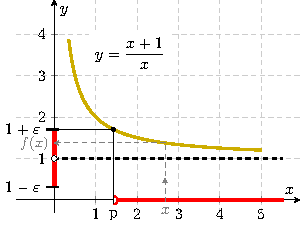
\includegraphics[width=0.45\linewidth]{mai_fig019.pdf}
    \captionof{figure}{K příkladu \ref{MAI:exam030}
    \cite[s.~119]{Brabec1989}
    \label{mai:fig019}}
    \par}
  \end{example}
\end{mdframed}
















    %-------------------------------------
    
    %-------------------------------------
      % !TeX spellcheck = cs_CZ
\begin{mdframed}[style=mdexam]
  \begin{example}\label{MAI:exam031}
    Je dána funkce \(f: f(x) = \frac{x + 1}{x}\). Sledujme její chování, když hodnoty argumentu
    \(x\) budou vzrůstat nade všechny meze neboli, jak říkáme, \(x\) se bude blížit k \(+\infty\)
    (což zapisujeme \(x \to + \infty\) (viz obr. \ref{mai:fig019}). Můžeme psát \(f(x) = 1 + 1/x\).
    Vzrůstají-li neomezeně hodnoty proměnné \(x\), blíží se hodnoty výrazu \(1/x\) čím dál tím více
    nule, takže funkční hodnoty \(f(x)\) jsou čím dál tím blíže číslu \(1\). V tomto případě píšeme
    \(lim_{x\to+\infty}f(x) = 1\) nebo \(f(x) \to 1\) pro \(x\to +\infty\) a říkáme, že funkce \(f\)
    má v bodě \(+\infty\) limitu rovnou \(1\). Přesně to znamená toto: Zvolíme-li libovolně malé
    \(\varepsilon > 0\), můžeme nalézt \(p > 0\) tak, že pro \(x > p\) platí \(\abs{f(x) - l} <
    \varepsilon\). (Viz obr. \ref{mai:fig019}.) Můžeme to říci i takto: Zvolíme-li libovolně okolí
    bodu \(1\), existuje okolí bodu \(+\infty\) tak, že pro každé \(x\) (konečné) z tohoto okolí je
    \(f(x)\) ve zvoleném okolí bodu \(1\).
    
    {\centering
    \captionsetup{type=figure}
  %   % !TeX spellcheck = cs_CZ
% xelatex -enable-write18 -shell-escape mai_fig020.tex
\documentclass[11pt]{standalone}
\usepackage{xltxtra}
\usepackage[usenames,x11names]{xcolor}
\usepackage{tikz}
  \usetikzlibrary{intersections}
  \usetikzlibrary{decorations.markings}
\usepackage{pgfplots}
  \pgfplotsset{compat=newest}
  
\usepackage{amsmath}

\begin{document}
  \begin{tikzpicture}[thick,scale=0.7, 
      every node/.style={transform shape},
      ]
  
  \tikzset{->-/.style={decoration={
    markings,
    mark=at position #1 with {\arrow{stealth}}},postaction={decorate}}}
    
    \begin{axis}[
      xmin = -2, xmax = 3.5, ymin = -2, ymax = 6,  % osy
      domain =-2:8,
      restrict y to domain=-1.5:6,
      axis equal image,
      grid = major,   % both
      grid style={line width=.1pt, draw=gray!20},
      major grid style={dashed, line width=.2pt, draw=gray!40},
      clip = true,
      clip mode=individual,
      xtick={-1,0,1,2,3,4}, % make steps of length 0.2
      ytick={-1,0,1,2,3,4,5,6,7,8}, 
      axis x line = middle,
      axis y line = middle,
      xlabel={$x$}, ylabel={$y$},
      enlarge y limits={rel=0.07},
      enlarge x limits={rel=0.07},
      ]
  
      \addplot[color=Gold3, samples=100, smooth, ultra thick, unbounded coords=jump,
               no markers, domain = -2:2, name path global=func1] 
         gnuplot{x^3};
  
      \node [fill=white] at (rel axis cs: 0.85,0.9) {\(y=x^3\)};
  
      \path[name path=line] (1.5,0) -- (1.5,6); 
          % Intersections points
          \path [name intersections={of=func1 and line,by={P1}}] (P1) node [] {};
          \draw[->-=.4, dashed, gray] (P1 |- 3,-0.05) node[below, fill=white] {\(x\)} -- (P1);
          \draw[->-=1,  dashed, gray] (P1) -- (P1 -| 0,3) 
            node[left=0.5cm, fill=white] {\small\(f(x)\)};
          \draw[dashed, gray] (P1 -| 0,3) + (-0.6cm,0cm) -- (P1 -| 0,3);
      \path[name path=line1] (0,1) -- (2,1); 
          % Intersections points
          \path [name intersections={of=func1 and line1, by={P1}}] (P1) node [] {};    
          \path (P1 |- 3,-0.1) node [below, fill=white] (X) {p} -- (P1) -- (P1 -| 0,3) 
              node[left, fill=white] (Y) {\(q\)};
  
      \draw[thick,red, fill=white] ([shift=(90:2mm)]X) 
           arc (270:360:1mm) node(x1) {} arc (360:450:1mm);
      \draw[dashed] (P1 |- 3,-0.1) -- (P1) -- (P1 -| 0,3);
      \draw[line width = 1pt,red] (x1 |- 3,0)  -- (3,0);
      
      \draw[thick,red] (0,1) -- (0,6);
      \draw[thick,red, fill=white] ([shift=(0:3.3mm)]Y) arc (0:180:1mm);;
    \end{axis}
  \end{tikzpicture}
\end{document}
    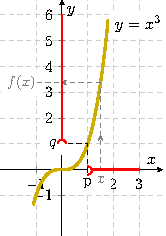
\includegraphics[width=0.35\linewidth]{mai_fig020.pdf}
    \captionof{figure}{K příkladu \ref{MAI:exam031}
    \cite[s.~119]{Brabec1989}
    \label{mai:fig020}}
    \par}
  \end{example}
\end{mdframed}
    %-------------------------------------
    
    V uvedených případech bychom mohli zkoumat i limity funkcí pro \(x \to - \infty\).  Všimněme si 
    ještě, že ve všech případech nebylo nutné, aby funkce \(f\) byla definována v bodě, ke kterému 
    se blíží hodnoty argumentu, ale bylo zapotřebí, aby funkce \(f\) byla definována v bodech 
    libovolně blízkých tomuto bodu. Tomuto požadavku bude vyhověno, jestliže daný bod, v němž 
    zkoumáme limitu, bude \emph{hromadným bodem definičního oboru}. Není ovšem nutné, aby funkce 
    byla definována v celém nějakém \emph{prstencovém okolí uvažovaného bodu}.
    
    Nechť \(a\) je bod, blízko kterého se pohybuje hodnota proměnné \(x\). Pro definici limity je 
    důležitý pojem \textbf{okolí bodu} \(a\) (obr. 2.16). Zvolme kladná čísla \(\delta_1\) a 
    \(\delta_2\). Nazýváme
    
    
      
  %================ Podkapitola: Spojitost funkce ==================================================
  \section{Spojitost funkce}
  
%} % tikzset
%~~~~~~~~~~~~~~~~~~~~~~~~~~~~~~~~~~~~~~~~~~~~~~~~~~~~~~~~~~~~~~~~~~~~~~~~~~~~~~~~~~~~~~~~~~~~~~~~~~
\printbibliography[title={Seznam literatury}, heading=subbibliography]
\addcontentsline{toc}{section}{Seznam literatury}          	
%-------------------- Theory_of_Derivatives -------------------------------------------------------
  % !TeX spellcheck = cs_CZ
%{\tikzset{external/prefix={tikz/MAI/}}
% \tikzset{external/figure name/.add={ch04_}{}}
%---------------------------------------------------------------------------------------------------
% file: Theory_of_Derivates.tex
%---------------------------------------------------------------------------------------------------
\chapter{Derivace funkce}\label{mai:IchapIV}
\minitoc

%============== Kapitola: Derivace funkce ==========================================================
  \section{Základní věty diferenciálního počtu}
    \subsection{Věta o největší (nejmenší) hodnotě funkce}
      V tomto článku uvedeme významné věty, zvané souhrně věty o \emph{střední hodnotě 
      diferenciálního počtu}, a dále pak ukázky jejich užití v matematické analýze.  Avšak dříve 
      než budeme tyto věty formulovat, uvedeme jedno důležité tvrzení, které sice bude mít v 
      dalších úvahách tohoto článku pomocnou úlohu, ale v teorii extrémů má i samostatný význam. 
      \cite[s.~186]{Brabec1989} 
      \begin{lemma}\label{MA1:lem_diff02}
        Nechť funkce $f:A\rightarrow\realset$ nabývá na množině $A$ své největší (nejmenší) hodnoty 
        na vnitřním bodě $c$ množiny $A$. Máli funkce $f$ v bodě $c$ derivaci, potom $f'(c)=0$.  
      \end{lemma}
      \begin{proof}
        Nechť např. $f(c)$ je největší hodnota funkce $f$ na množině $A$, takže $f(x)\leq f(c)$ pro $\forall x\in A$. Potom pro $x\in A, x<c$, je 
        $$\frac{f(x)-f(c)}{x-c}\geq 0$$
        a tedy
        $$f'_{-}(c)=\lim_{x\rightarrow c^-}\frac{f(x)-f(c)}{x-c}\geq0$$ 
        Dále pro $x\in A, x>c$, je
        $$\frac{f(x)-f(c)}{x-c}\leq 0$$ 
        a proto
        $$f'_{+}(c)=\lim_{x\rightarrow c^+}\frac{f(x)-f(c)}{x-c}\leq0$$
        Platí tedy
        $$f'_{+}(c)\leq f'_{-}(c)\geq f'_{-}(c).$$ 
        Avšak $f'_{+}(c)=f'_{-}(c)= f'(c)$. Odtud plyne $f'(c)=0$. 
      \end{proof}
      
    \subsection{Věty o střední hodnotě}
      \begin{lemma}\label{MA1:lem_diff03}
        \textbf{Rolleova věta}\footnote{Michel Rolle [Mišel Rol] (1652-1719) Francouzský matematik} Nechť funkce $f$ má tyto vlastnosti:
          \begin{enumerate}
            \item je spojitá na uzavřeném intervalu $\langle a,b\rangle$;
            \item má derivaci (vlastní či nevlastní) na otevřeném intervalu $(a,b)$;
            \item platí $f(a)=f(b)$.
          \end{enumerate}
        Potom v otevřeném intervalu $(a,b)$ existuje aspoň jeden bod $\xi$ takový, že $f'(\xi)=0$.   
      \end{lemma}
      \begin{proof}
        Protože je funkce $f$ je na uzavřeném intervalu $\langle a,b\rangle$ spojitá, nabývá v 
        tomto intervalu své největší hodnoty $M$,své nejmenší hodnoty $m$. Přitom ovšem platí:
        \begin{equation}\label{MA1:eq_diff02}
          m\leq f(x) \leq M, \qquad x\in\langle a,b\rangle.
        \end{equation}
        Nyní mohou nastat dva případy: 
        \begin{enumerate}
          \item funkce $f$ nabývá $M$ i $m$ právě v krajních bodech intervalu $\langle a,b\rangle$. Podle předpokladu 3 věty \ref{MA1:lem_diff03}
                však potom platí $f(a)=f(b)=m=M$. Vzhledem ke vztahu \ref{MA1:eq_diff02} odtud plyne, že funkce $f$ je konstantní na intervalu
                $\langle a,b\rangle$ a tedy $f'(x)=0$ dokonce v každém bodě $x\in(a,b)$
          \item Funkce $f$ nabývá apsoň jedné z hodnot $M$, $m$ v některém vnitřním bodě $\xi$ intervalu $\langle a,b\rangle$. Potom podle 
          věty \ref{MA1:lem_diff02} je $f'(\xi)=0$.         
        \end{enumerate}        
      \end{proof}
      \begin{note}
        Rolleova věta sama zaručuje jen existenci aspoň jednoho bodu $\xi\in(a,b)$, ve kterém je fe 
        $f'(\xi)=0$. Neumožňuje však ani určení tohoto bodu (nebo bodů), ani stanovení jejich počtu 
      \end{note}
      
      \begin{note}
        Na obr. \ref{MAI:fig_027} je ilustrován geometrický význam Rolleovy věty. Graf funkce na 
        tomto obrázku má v bodech $\xi_1$, $\xi_2$, v nichž je $f'(\xi_1)=f'(\xi_2)=0$ tečny 
        rovnoběžné s osou $x$. 
        \begin{figure}[ht!] %\ref{MAI:fig_027}
          \centering
          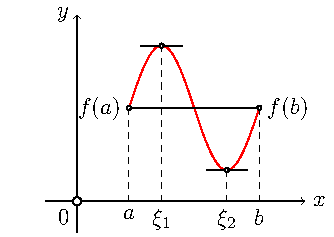
\includegraphics[width=0.7\linewidth]{mai_fig027.pdf}
          \caption{K výkladu Rolleovy věty}
          \label{MAI:fig_027}
        \end{figure}
      \end{note}
      
      Z Rolleovy věty plyne důležitá věta:
      
      \begin{lemma}\label{MA1:lem_diff04}
        (\textbf{Cauchyova věta}). Nechť funkce $f$ a $g$ mají tyto vlastnosti:
        \begin{enumerate}
          \item  Jsou spojité na uzavřeném intervalu $\langle a,b\rangle$,
          \item  v každém bodě $x\in(a,b)$ existuje derivace $f'(x)$ (vlastní či nevlastní) a vlastní derivace $g'(x)$,
          \item  $g'(x)\neq0$ na $(a,b)$
        \end{enumerate}
        Potom v otevřeném intervalu $(a,b)$ existuje aspoň jeden bod $\xi$, pro který platí
        \begin{equation}\label{MA1:eq_diff03}
          \frac{f(b)-f(a)}{g(b)-g(a)} = \frac{f'(\xi)}{g'(\xi)}.
        \end{equation} 
      \end{lemma} 
      
      \begin{proof}
        Poznamenejme především, že z předpokladu 3 $g'(x)\neq0$ pro $x\in(a,b)$ a z předpokladu 
        spojitosti funkce $g$ na uzavřeném intervalu $\langle a,b\rangle$ ihned vyplývá vztah 
        $g(b)- g(a)\neq 0$. Kdyby totiž bylo $g(b)=g(a)$, potom by podle \emph{Rolleovy věty} 
        \ref{MA1:lem_diff03} existoval aspoň jeden bod $\eta\in(a,b)$ takový že $g'(\eta)=0$. To 
        však by byl spor s předpokladem $g'(x)\neq0$ pro každý bod $x\in(a,b)$. Proto má smysl 
        podíl na levé straně rovnosti \ref{MA1:eq_diff03}
        
        K vlastnímu důkazu Cauchyovy věty zavedeme takovou pomocnou funkci $F$, aby splňovala podmínky Rolleovy věty. Definujme ji pro $x\in\langle a,b\rangle$ předpisem
        \begin{equation}\label{MA1:eq_diff04}
          F(x)=[f(b)-f(a)]\cdot[g(x)-g(a)]-[f(x)-f(a)]\cdot[g(b)-g(a)].
        \end{equation}
        Snadno ověříme, že tato funkce skutečně splňuje podmínky Rolleovy věty na intervalu $\langle a,b\rangle$:
        \begin{itemize}
          \item Je spojitá na intervalu $x\in\langle a,b\rangle$, což je důsledkem spojitosti  
                funkce $f$ a $g$ na intervalu $x\in\langle a,b\rangle$ ,
          \item má derivaci $F'$ na otevřeném intervalu $(a,b)$, což plyne z existence derivace  
                $f'$ a $g'$ funkce $f$ a $g$ na  intervalu $(a,b)$,
          \item $F(a)=F(b)=0$ 
        \end{itemize}
        Platí tedy i závěr Rolleovy věty pro funkci $F$, tj. na intervalu $(a,b)$ existuje aspoň 
        jeden bod $\xi$, pro který $F'(\xi)=0$. Zderivujeme-li funkci $F$, dostaneme (dosadíme-li 
        $x=\xi$): $$F'(\xi)=[f(b)-f(a)]g'(\xi)-f'(\xi)[g(b)-g(a)]=0$$ Odtud již plyne rovnost 
        \ref{MA1:eq_diff03}                  
      \end{proof}
      
      Významným zvláštním případem Cauchyovy věty je další věta, která se častěji používá.
      
      \begin{lemma}\label{MA1:lem_diff05}
        (\textbf{Lagrangeova věta})\footnote{Joseph Louis Lagrange [lagránž] (1736-1813), francouzský matematik}. Nechť funkce má tyto vlastnosti:
        \begin{itemize}
          \item Je spojitá na intervalu $\langle a,b\rangle$,
          \item má derivaci (vlastní či nevlastní) na otevřeném intervalu $(a,b)$. 
        \end{itemize} 
        Potom existuje v otevřeném intervalu $(a,b)$ aspoň jeden bod $\xi$, pro který platí 
        \begin{equation}\label{MA1:eq_diff05}
           \frac{f(b) - f(a)}{b - a} = f'(\xi),  
        \end{equation}  
        či-li
        \begin{equation}\label{MA1:eq_diff06}
           f(b) - f(a) = f'(\xi)(b-a),  
        \end{equation}           
      \end{lemma}
      
      \begin{proof}
        Tvrzení této věty je důsledkem tvrzení \emph{Cauchyovy věty}, a to pro případ $g(x)=x$. 
        Protože $g'(x)=1$ dokonce všude, jsou splněny všechny tři podmínky Cauchyovy věty. Proto 
        platí i závěr této věty, z něhož pro náš případ již plyne vzorec \ref{MA1:eq_diff05} a tedy 
        i vzorec \ref{MA1:eq_diff06}.  
      \end{proof}
      
      \begin{note}
        Podobně jako je Lagrangeova věta zvláštním případem věty Cauchyovy, je Rolleova věta zvláštním případem Lagrangeovy věty, a to přo případ, že $f(a)=f(b)$.
      \end{note}
      
      \begin{note}
        Lagrangeova věta se často nazývá \emph{větou o přírůstku funkce}, protože vzorcem \ref{MA1:eq_diff06} se vyjadřuje \emph{přírůstek funkce}, tj rozdíl $f(b)-f(a)$. 
        Všechny tři uvedené věty, tj. věta Rolleova, Cauchyova a Lagrangeova, se v literatuře nazývá souhrně \textbf{věty o střední hodnotě diferenciálního počtu}.
      \end{note}
      
      \begin{note}
        Na obr. ** je ilustrován geometrický význam Lagrangeovy věty. Podíl na levé straně rovnosti 
        \ref{MA1:eq_diff05}, tj. číslo $\frac{f(b) - f(a)}{b - a}$ je směrnice sečny $s$, spojující 
        body $A$, $B$ grafu funkce  $f$, které odpovídají krajním bodům intervalu $\langle 
        a,b\rangle$. Podle tvrzení Lagrangeovy věty existuje v otevřeném intervalu $(a,b)$ aspoň 
        jeden bod $\xi$ tak, že tečna grafu funkce $f$ v příslušném jeho bodě je rovnoběžná s 
        přímkou $s$.  
      \end{note}
      
      \begin{note}
        Z Lagrangeovy věty vyplývá toto tvrzení: Nechť funkce $f$ vyhovuje na intervalu $\langle a,b\rangle$ podmínkám Lagrangeovy věty a $x_1$, $x_2$ jsou dva libovolné různé body
        intervalu $\langle a,b\rangle$. Potom v otevřeném intervalu s krajnímy body $x_1$, $x_2$ existuje aspoň jeden bod $\xi$, pro který platí Lagrangeův vzorec:   
        \begin{align}
          f(x_2) - f(x_1)                  &= f'(\xi)(x_2-x_1) \label{MA1:eq_diff07} \\ 
          \frac{f(x_2) - f(x_1)}{x_2-x_1}  &= f'(\xi)          \label{MA1:eq_diff08}      
        \end{align}
        Potom bod $\xi$ lze vyjádřit takto:
        \begin{equation}\label{MA1:eq_diff09}  
          \xi = x_1 + \vartheta(x_2-x_1), \qquad \text{kde }\vartheta\in(0,1). 
        \end{equation}
        Označíme-li $x_2-x_1=h$, můžeme vzorec \ref{MA1:eq_diff07} napsat ve tvaru
        \begin{equation}
          f(x_1+h) - f(x_1)= f'(x_1 + \vartheta h)h, \qquad \text{kde }\vartheta\in(0,1). 
        \end{equation} 
      \end{note}       
          
    \subsection{Některé důsledky Lagrangeovy věty}
      Lagrangeova věta, má některé významné důsledky, které nyní uvedeme \cite[s.~189]{Brabec1989}:
      \begin{lemma}\label{MA1:lem_diff06} 
        Nechť funkce $f$ vyhovuje podmínkám Lagrangeovy věty a navíc nechť $f'(x)=0$ pro všechna 
        $x\in(a,b)$. Potom funkce $f$ je prostá na intervalu $\langle a,b \rangle$. 
      \end{lemma}
      \begin{proof}
        Necť $x_1, x_2$ jsou libovolné dva různé body intervalu $\langle a,b \rangle$. Potom podle 
        Lagrangeova vzorce \ref{MA1:eq_diff04} platí 
        \begin{equation}
          f(x_2) - f(x_1) = f'(\xi)(x_2-x_1) \neq0
        \end{equation}
        neboť $f'(\xi)\neq 0$ dle předpokladu.
      \end{proof}
      
      \begin{lemma}\label{MA1:lem_diff01}
        Funkce $f$ je konstantní na intervalu $(a,b)$, právě když má na tomto intervalu derivaci a platí $f'(x) = 0$ pro všechna $x\in(a,b)$. 
      \end{lemma}
      \begin{proof} Tedy
        \begin{itemize}
          \item Je-li funkce $f$ konstantní na intervalu $(a,b)$, pak je $f'(x) = 0$ pro všechna  
                $x\in(a,b)$, jak již víme.
          \item Nechť $f'(x) = 0$ pro všechna $x\in(a,b)$. Dokažme, že pro každé dva body $x_1, 
                x_2  \in(a,b)$, $x_1\neq x_2$, platí $f(x_1) = f(x_2)$. Z existence
                derivace vyplývá spojitost funkce a jsou tedy splněny podmínky Lagrangeovy věty na 
                každém intervalu $\langle x_1, x_2\rangle\subset(a,b)$. Podle vzorce 
                \ref{MA1:eq_diff04} tedy platí $f(x_2)-f(x_1)f'(\xi)(x_2-x_1)$, $\xi\in(x_1,x_2)$. 
                Protože podle předpokladu je $f'(x)=0$ pro $\forall x\in(a,b)$, platí $f(x_1) 
                -f(x_2)=0$, tj. $f(x_1)=f(x_2)$  
        \end{itemize}
      \end{proof}
      
%} % tikzset
%---------------------------------------------------------------------------------------------------
\printbibliography[heading=subbibliography]
\addcontentsline{toc}{section}{Seznam literatury}
%-------------------- Differential Calculus applications ------------------------------------------
  % !TeX spellcheck = cs_CZ
%{\tikzset{external/prefix={tikz/MAI/}}
% \tikzset{external/figure name/.add={ch05_}{}}
%---------------------------------------------------------------------------------------------------
% file: Differential_Calculus_applications.tex
%---------------------------------------------------------------------------------------------------
\chapter{Aplikace diferenciálního počtu}\label{chap:Apl_dif_poc}
\minitoc

%================Kapitola: Aplikace diferenciálního počtu =========================================
Diferenciální počet má rozsáhlou oblast užití. V této kapitole ukážeme použití výsledků předchozích 
kapitol k vyšetřování průběhu funkce a vlastnosti rovinných křivek. 
  \section{Průběh funkce}
    Pomocí derivace můžeme studovat vlastnosti funkce, které usnadní vyšetřování jejího průběhu.  
    \subsection{Monotonie funkcí}
      Jednou z důležitých vlastností funkce je její \textquotedblleft monotonie\textquotedblright, 
      kterou jsme definovali již v odst. \ref{MA1:subsec_vlastnosti_funkce} kap. 
      \ref{mai:IchapLimit}. Proto je při vyšetřování průběhu funkce důležité určit množiny (často 
      jsou to intervaly), na nichž je funkce monotónní, jinak řečeno, najít \textquotedblleft 
      intervaly monotonie funkce\textquotedblright (viz \cite[s.~208]{Brabec1989}). 
    \begin{enumerate}
      \item Zjistíme \textbf{definiční obor funkce}, vyjádříme jej v intervalech a z nich poznáme,  
            kde je funkce \textbf{spojitá}. Funkce je spojitá v $(a,b)$ pro každý bod tohoto 
            intervalu, když$|f(x)-f(c)|<\varepsilon$, kde $\varepsilon>0$ je libovolně zvolené 
            číslo, a pro všechna $x$ z okolí bodu $c$ je $|x-c|<\delta$, kde $\delta>0$ je na 
            $\varepsilon$ nezávislé.
      \item Určíme, je-li funkce \textbf{lichá} $f(-x)=-f(x)$ nebo \textbf{sudá} $f(-x)=f(x)$.   
            Je-li funkce lichá, je souměrná podle středu souměrnosti (obyčejně to bývá počátek 
            souřadnic $xy$), je-li sudá, je souměrná podle osy $y$.
      \item Určíme \emph{průsečíky křivky s osami pravoúhlých souřadnic}. Body, ve kte\-rých 
            křivka  protíná osu $x$ spolu s body, ve kte\-rých není křivka spojitá, rozlišují 
            intervaly, v nichž je graf křivky nad osou $x$ od intervalů, ve kterých je graf křivky 
            pod osou $x$.
      \item V krajních bodech definičních intervalů, ve kterých je funkce spojitá, stano\-víme 
      \emph{limity funkce} a dále $$\lim_{x \to \pm \infty}f(x).$$
      \item Vypočítáme $f'(x)$ a $f''(x)$, abychom zjistily, kde je funkce \emph{rostoucí}     
            $f'(x)>0$, \emph{klesající} $f'(x)<0$ a kde jsou \emph{lokální extrémy}. Dostaneme-li 
            dosazením kořenů rovnice $f'(x)=0$ do $f''(x)$ hodnotu $f''(x)>0$, má funkce lokální 
            minimum, při $f''(x)<0$ má funkce lokální maximum. V intervalech, kde $f''(x)>0$, je 
            křivka \textbf{konvexní (vypuklá)}, kde $f''(x)<0$, je křivka \textbf{konkávní 
            (vydutá)}. Body, v nichž $f''(x)$ mění znaménko, jsou \textbf{inflexní body}. Najdeme 
            je tak, že stanovíme hodnoty $x$, pro které je $f''(x)=0$ nebo neexistuje. Číslo $c$ je 
            inflexní bod, když existuje takové okolí bodu $c$, že pro $x>c$ je oblouk křivky 
            konvexní a pro $x<c$ konkávní. Je nutné si uvědomit, že když má $f'(x)$ konečnou 
            derivaci, je inflexní bod $c$ taky nulovým bodem druhé derivace čili kořenem rovnice 
            $f''(x)=0$. Obrácená věta neplatí, tj. z $f''(x)=0$ nevyplývá, že v bodě $c$ má $f'(x)$ 
            extrém a že bod $c$ je inflexním bodem.
      \item \textbf{Asymptota} je tečna křivky $f(x)$, jejíž bod dotyku je v nekonečnu. Platí-li  
            $$\lim_{x \to a}f(x) =  \pm\infty,$$ je přímka $x=a$ její asymptotou. Jinak asymptoty 
            mají rovnici $y=kx+q$, kde $x$ a $y$ jsou souřadnice bodů na asymptotách. Existují-li 
            konečné limity $$\lim_{x \to \pm\infty}\frac{f(x)}{x}=k$$  a $$\lim_{x \to 
            \pm\infty}[f(x)-kx] =q$$ pak je asymptotou přímka $y=kx+q$. Můžeme-li rovnici křivky 
            rozložit (tj. rozložit její pravou stranu, oby\-čejně dělením čitatele jmenovatelem, 
            má-li tvar zlomku) na dvě části, z nichž jedna má tvar $kx+q$ a druhá zbytek 
            $\varphi(x)$, tj. $f(x)=kx+q+\varphi(x)$ a $\varphi(x)_{x\rightarrow 
            \pm\infty}\rightarrow 0$, je přímka $y=kx+q$ asymptotou.
      \item Zpřesnění grafu křivky provedeme sestavením tabulky souřadnic dalších bodů křivky,  
            tj. ke zvoleným hodnotám $x$ (z definičního oboru funkce) vypočítáme hodnoty $y$. Do 
            dalších řádků tabulky zapíšeme hodnoty  $f'(x)$ a $f''(x)$, ve kterých intervalech je 
            funkce \emph{rostoucí}, ve kterých \emph{klesá}, kde je \emph{vypuklá}, kde je 
            \emph{dutá}, kde jsou \emph{lokální extrémy}, \emph{inflexní body} apod., 
            případně sestavíme dílčí tabulky pro jednotlivé \emph{charakteristické vlastnosti} vyšetřované funkce.
    \end{enumerate}
    %-------------------- EXAM001 --------------------------------------
    % !TeX spellcheck = cs_CZ
\begin{mathexam}{Vyšetřete průběh funkce \(f(x):y=\frac{1+x^2}{1-x^2}\)}{exam003}
  \begin{enumerate}[noitemsep]
    \item Definiční obor $D_f=\realset-\{±1\}=(-\infty,-1)\cup(-1,1)\cup(1,+\infty)$
    \item Funkce je sudá $$f(-x)=f(x): \frac{1+x^2}{1-x^2}=\frac{1+(-x)^2}{1-(-x)^2}.$$ Funkce není
        periodická.
    \item Stanovíme funkční hodnoty v krajních bodech definičního obor $1, -1$ a v nevlastních
        bodech $-\infty,+\infty$.Protože je funkce \textbf{sudá}, omezíme se jen na vyšetřování
        nezáporné části. Nejprve vlastnosti funkce v okolí bodu $1$. Ten nepatří do $D_f$ a proto
        určíme limity funkce v pravém a levém okolí tohoto bodu. $$\lim_{x\to
        1_{-}}=\frac{1+x^2}{1-x^2}.$$ Pro výpočet limity použijeme substituci $y=1-x^2$: 
        $$\lim_{y\to0+}\frac{2-y}{y}=+\infty$$ \footnote{$\lim_{x\to0_+}\frac{1}{x}=\infty$} proto
        
        $$\lim_{x\to1_{-}}\frac{1+x^2}{1-x^2}=+\infty.$$ Obdobně dojdeme k
        $$\lim_{x\to1_+}\frac{1+x^2}{1-x^2}=-\infty.$$ A konečně v nevlastních bodech $±\infty$ je
        limita $$\lim_{x\to±\infty}\frac{1+x^2}{1-x^2} = \lim_{x\to\pm\infty}\frac{1}{1-x^2} +
        \lim_{x\to\pm\infty}\frac{x^2}{1-x^2}=0-1=-1.$$ Výpočtem limit jsme zároveň určili dva
        absolutní (globální) extrémy a jeden lokální:
        \begin{itemize}
          \item v intervalu $(-1,1)$ má funkce maximum $\infty$ a minimum $1$,
          \item v intervalech $(-1,1)\cup(1,+\infty)$ má funkce minimum $-\infty$ a maximum $-1$.
        \end{itemize}
    \item Nyní vyšetříme zda, případně kolik a jaké, má funkce $f(x)$ průsečíky s osami souřadnic. S
        osou $x$ nemá funkce žádné průsečíky, protože pro $y=0$ není definována
        $H_f=\realset-\{-1,1\rangle$. Pro $x=0$ je $y=\frac{1+0^2}{1-0^2}=1$, proto má $f(x)$ právě
        jeden průsečík s osou $y$ a to $[0,1]$.
    \item Zatím jsme zjistili, že naše funkce není definována v bodech $1$ a $-1$ a proto není
        spojitá v  $\realset$. Nevíme však, jaký je její průběh v jednotlivých intervalech
        definičního oboru.  Abychom získali názornější představu o průběhu funkce, zjistíme má-li
        derivaci.
        \begin{align*}
          y' &= \frac{(1+x^2)'(1-x^2 )-(1+x^2)(1-x^2 )'}{(1-x^2)^2} \\
          y' &= \frac{2x(1-x^2 )-(1+x^2 )(-2x)}{(1-x^2 )^2}         \\
          y' &= \frac{4x}{(1-x^2 )^2}
        \end{align*}
        Protože má vlastní derivaci\footnote{$f(x)$ je spojitá v intervalech $(-\infty,-1),
        (-1,1),(1,\infty)$  věta s spojité funkci}, můžeme určit její vlastnosti v intervalech
        $\langle0,1)$ a $(1,\infty)$. V těchto intervalech je $y'>0$ a proto jde o funkci ryze
        monotónní, rostoucí \footnote{Plyne z věty o postačujících podmínkách ryzí monotónnosti
        funkce na intervalu} v daných intervalech \footnote{V intervalech
        $(-\infty,-1),(-1,0\rangle$ je funkce klesající.}. Výpočtem zjistíme druhou derivaci funkce.
        Ta nám pomůže určit další extrém v intervalu $\langle0,1)$ a zároveň vyšetřit
        \textbf{konkávnost} a \textbf{konvexnost}.
        \begin{align*}
          y'' &= \frac{(4x)' (1-x^2 )^2-(4x)(1-2x^2+x^4 )'}{(1-x^2 )^4}  \\
          y'' &= \frac{4(1-2x^2+x^4 )-4x(-4x+4x^3 )}{(1-x^2 )^4}         \\
          y'' &= \frac{4(1-x^2 )(3x^2+1)}{(1-x^2 )^4}                    \\
          y'' &= \frac{4(3x^2+1)}{(1-x^2 )^3}
        \end{align*}
        Abychom mohli určit lokální extrém funkce $f(x)$ v intervalu $\langle0,1)$, pomocí druhé
        derivace, musíme najít kořeny rovnice $f' (x)=0$. V našem případě
        $$y'=\frac{4x}{(1-x^2)^2}\Rightarrow\frac{4x}{(1-x^2)^2}=0\rightarrow x_0=0,$$ tento kořen
        \footnote{stacionární bod}  pak dosadíme do druhé derivace, tj. 
        $$y''(0)=\frac{4(3\cdot0^2+1)}{(1-0^2 )^3}=4,$$ protože je $f''(x)>0$, má v bodě $x_0$
        lokální minimum. Můžeme rovněž konstatovat, že funkce nemá inflexní body \footnote{Pro
        existenci inflexního bodu je nutné splnění jedné z podmínek a to buď $f''(x_0)=0$, nebo
        $f''(x_0)$ neexistuje.}. Konkávnost a konvexnost funkce v intervalech $\langle0,1)$ a
        $(1,\infty)$ vyšetříme pomocí vlastností druhé derivace funkce. Tedy
        \begin{itemize}
          \item $\langle0,1): y''=\frac{4(3x^2+1)}{(1-x^2 )^3} >0 \Rightarrow$ funkce je v tomto
                intervalu \textbf{konvexní},
          \item $(1,\infty): y''=\frac{4(3x^2+1)}{(1-x^2 )^3} <0 \Rightarrow$ funkce je v tomto
                intervalu \textbf{konkáv\-ní}.
        \end{itemize}
    \item Z předchozích výpočtů plyne, že křivka má asymptoty $y=-1,x=\pm1$.
  \end{enumerate}
  {\centering \captionsetup{type=figure}          % %\ref{MAI:fig_028}
    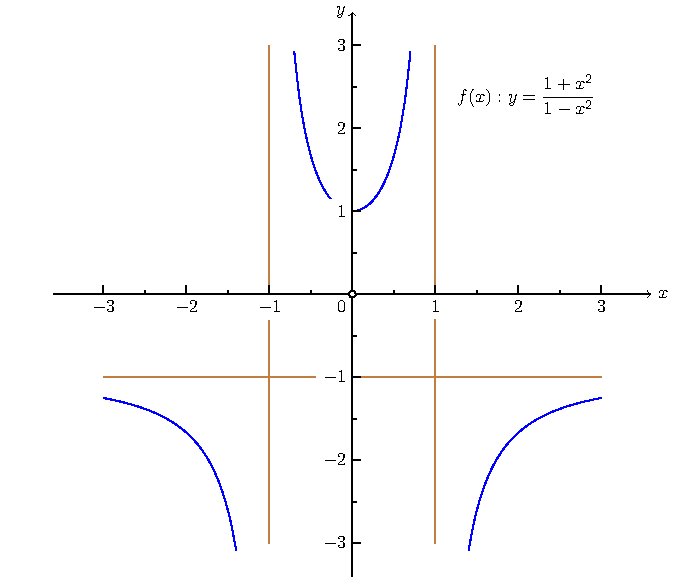
\includegraphics[width=1\linewidth]{mai_fig028.pdf}
    \captionof{figure}{Graf funkce $f(x):y=\dfrac{1+x^2}{1-x^2}$}
    \label{MAI:fig_028}
  \par}
\end{mathexam}  
    %-------------------------------------------------------------------

%} %tikzset
%---------------------------------------------------------------------------------------------------
\printbibliography[heading=subbibliography]
\addcontentsline{toc}{section}{Seznam literatury} 
%--------------------Primitive Functions ----------------------------------------------------------
  % !TeX spellcheck = cs_CZ
%{\tikzset{external/prefix={tikz/MAI/}}
% \tikzset{external/figure name/.add={ch06_}{}}
%---------------------------------------------------------------------------------------------------
% file: chap_PrimitiveFce.tex
%---------------------------------------------------------------------------------------------------
%============================ Primitivní funkce ====================================================
\chapter{Primitivní funkce}
\minitoc

  %----------------------------Neurčitý integrál----------------------------------------------------
  \section{Motivace}
    Problém \emph{neurčitého integrálu}, neboli \textbf{primitivní funkce}, lze vyložit velmi 
    jednoduše: Máme podezření, že zadaná funkce \(f(x)\) vznikla derivováním jisté, zatím neznámé, 
    funkce \(F(x)\). Dokážeme ji najít? 
  
    K danému problému můžeme přistupovat také fyzikálně: Zavedením pojmu derivace funkce jsme 
    motivovali důležitým požadavkem definovat okamžitou rychlost pohybu bodu po přímce. Existuje 
    přirozeně i požadavek opačný, tj. nalézt zákon dráhy pohybu bodu po přímce, je-li dána jeho 
    okamžitá rychlost jako funkce času \cite[s.~253]{Brabec1989}. Vše si ukážeme na následujícím 
    příkladu:  
   
    \begin{example}
      Je dána okamžitá rychlost $v$ pohybu bodu po přímce (ose) $x$ rovnicí $v(t) = 2t + 1$, 
      $t\in\langle -\infty,+\infty \rangle$. Najděte zákon dráhy pohybu, je-li známo, že v čase $t 
      = 0$ měl bod polohu $x = x_0$.
      \newline
      \textbf{řešení:}\newline
      Označíme-li $x(t)$ polohu bodu v okamžiku $t$, pak $v(t) = \frac{dx}{dt}$. Hledáme tedy 
      funkci $x = x(t)$, pro níž platí 
      \begin{align}
        \frac{dx}{dt} &= 2t + 1 \qquad x(0) = x_0.  \nonumber \\ 
        \shortintertext{Je ihned patrné, že první podmínce vyhovuje nekonečně mnoho funkcí}
        x(t)          &= t^2 + t + C,           \label{MA:int_ex_09}    \\ 
        \shortintertext{ kde $C$ je libovolná konstanta. Funkce, která splňuje i druhou podmínku 
          (říkáme ji též počáteční podmínka), najdeme z rovnice \ref{MA:int_ex_09} dosazením dané podmínky 
          $t = 0,\ x = x_0$. Dostaneme $x_0 = C$. Dosazením do \ref{MA:int_ex_09} za $C$ plyne hledaný 
          zákon dráhy}
        x(t)          &= t^2+t+x_0.                 \nonumber 
        \shortintertext{Jednoduchou zkouškou se přesvědčíme, že tato funkce splňuje obě dané podmínky a 
          zároveň vidíme, že hledaná primitivní funkce daných vlastností je jediná.}  \nonumber
      \end{align}
    \end{example} 
    Každé takové funkci, jejíž derivací je daná funkce, budeme říkat \emph{primitivní funkce} k 
    dané funkci. Na uvedeném příkladě je patrné, že k dané funkci může existovat nekonečně mnoho 
    primitivních funkcí. Množinu všech primitivních funkcí se často nazývá \textbf{neurčitým 
    integrálem}. Po tomto názorném uvedení do problému přejděme k přesné formulaci základních pojmů.
    
    \begin{definition} 
      Funkce $F: J\rightarrow \realset$, kde $J\subset \realset$ je interval, se nazývá primitivní 
      funkce k funkci \(f\) na intervalu \(J\) právě když, pro všechna $x\in J$ je $F'(x) = f(x)$ 
      (v krajních bodech intervalu \(J\), pokud k němu patří, jde o derivace jednostranné).
    \end{definition}
    
    \begin{example} 
      K funkci $\sin x$ je primitivní funkcí na libovolném intervalu $J\subset(-\infty,+\infty)$ 
      funkce $-\cos x$, protože $(-\cos x)' = \sin x$. Ale též funkce $3-\cos x$ je primitivní 
      funkcí k funkci $\sin x$, protože $(3 - \cos x)' = \sin x$ pro všechna $x\in(-\infty, 
      \infty)$.
    \end{example}
    
    Je vidět, že rozdíl dvou primitivních funkcí k téže funkci je konstanta. To není náhoda, jak 
    potvrzuje následující věta:
    
    \begin{lemma}
      \begin{enumerate}
        \item Je-li funkce $F$ primitivní funkcí k funkci \(f\) na intervalu \(J\) a \(c\) reálná  
              konstanta, pak i funkce $G = F + c$ je primitivní funkcí k funkci \(f\) na intervalu 
              \(J\).
        \item Jsou-li funkce $F$ a $G$ primitivní funkce k funkci \(f\) na intervalu \(J\), pak 
        funkce
              $F-G$ je na intervalu \(J\) konstantní.
      \end{enumerate} 
      \begin{proof}
        Tvrzení a) plyne z definice protože $G'(x) = [F(x) + c] = F'(x) = f(x)$ pro všechna $x\in
        J$. Tvrzení b) je důsledkem věty \ref{MA1:lem_diff01}.
      \end{proof}
    \end{lemma}
    Neurčitost vyplývá právě z toho, že primitivní funkce není dána jednoznačně, je určena až na 
    konstantu. Značíme
    \begin{equation*}
      \boxed{F(x) = \int f(x)\dx + C}
    \end{equation*}
        
    Jak ale primitivní funkce hledat? V jednoduchých příkladech poslouží tabulka derivací, již 
    čteme „zprava doleva“. (Je dobré si ji uložit do paměti.) Tabulka však pokryje jen velmi málo 
    případů, pouze elementární funkce. Je tedy třeba najít metody, jak při hledání primitivních 
    funkcí postupovat. Nejprve však uvedeme dvě základní pravidla pro primitivní funkce, která 
    plynou z pravidel pro derivování:
    \begin{align}
      \int[f(x)\pm g(x)]\dx &= \int[f(x)\pm g(x)]\dx + \int[f(x)\pm g(x)]\dx \label{MA1:eq_int10} \\
      \int cf(x)\dx         &= c \int f(x)\dx, \qquad \text{\(c\) je konstanta.} \label{MA1:eq_int11}
    \end{align}
  
  \section{Tabulka neurčitých integrálů}\label{MA:chap_tabINT}
    Pokud není nic uvedeno, platí vzorce pro všechna \(x\) a pro všechny hodnoty uvedených
    konstant. Místo platí pro \(x\) z intervalu \((-\infty,0),(0,+\infty)\) píšeme stručně
    \(x\neq0\) apod. Literatura: \cite[p.~396]{Rektorys1963}.
  
    \begin{flalign}
      & \int 0\dx = c                                        &         \label{MA:baseInt01}     \\
      & \int a\dx = ax+c                                     &         \label{MA:baseInt02}     \\
      & \int x^n\dx = \frac{x^{n+1}}{n+1}+c, \,              &         \label{MA:baseInt03}     \\
      & \qquad\text{kde}\begin{cases}
          \forall x\in\realset,\,n\in\naturalset, n>0,         \\
          \forall x\in\realset-\{0\},\,n\in\naturalset, n<-1,  \\
          \forall x>0,\,n\in\realset\,\,n\notin\naturalset
        \end{cases}                                          &         \nonumber               \\
      & \int\frac{1}{x}\dx = 
            \ln\abs{x}+c \hspace{1ex}\forall x\neq0          &         \label{MA:baseInt04}     \\
      & \int e^x \dx       = e^x+c                           &         \label{MA:baseInt05}     \\
      & \int\ln x\dx       = 
          x\ln x - x + c \hspace{1ex}\forall x>0             &         \label{MA:baseInt06}     \\
      & \int a^x \dx     =
          \frac{a^x}{\ln a}+c 
          \hspace{1ex}\forall a>0,\,a\neq1                   &         \label{MA:baseInt07}     \\
      & \int \sin x \dx  = -\cos x                           &         \label{MA:baseInt08}     \\
      & \int \cos x \dx  =  \sin x                           &         \label{MA:baseInt09}     \\
      & \int\frac{1}{\cos^2x}\dx =  \tan x+c 
           \hspace{1ex}\forall x\neq(2k+1)\pi,\,k\in\naturalset &      \label{MA:baseInt10}     \\ 
      & \int\frac{1}{\sin^2x}\dx     =  -\cotg x+c
         \hspace{1ex}\forall x\neq k\pi,\,k\in\naturalset    &         \label{MA:baseInt11}     \\
      & \int\frac{1}{\sqrt{1-x^2}}\dx =
          \begin{cases}
            +\arcsin x + c         \\
            -\arccos x + c
          \end{cases} 
          \forall x\in(-1,1)                                 &         \label{MA:baseInt12}     \\
      & \int\cosh\dx = \sinh x + c                           &         \label{MA:baseInt13}     \\
      & \int\sinh\dx = \cosh x + c                           &         \label{MA:baseInt14}     \\
      & \int\frac{1}{1+x^2}\dx = \arctan x + c               &         \label{MA:baseInt15}     \\
      & \int \frac{1}{\sqrt{x^2 + 1}}\dx =
          \begin{cases}
            \ln(x + \sqrt{x^2+1}) + c         \\
            \sinh^{-1}x + c 
          \end{cases}                                        &         \label{MA:baseInt16}     \\ 
      & \int \frac{1}{\sqrt{x^2 - 1}}\dx =
          \begin{cases}
            \ln(x + \sqrt{x^2-1}) + c         \\
            \cosh^{-1}x + c \hspace{4ex}x\in(1,+\infty) 
          \end{cases}                                        &         \label{MA:baseInt17}     \\
      & \int\frac{1}{\sqrt{x^2+a^2}}\dx 
        = \sinh^{-1} \frac{x}{a} = \ln (x+\sqrt{x^2+a^2})    &         \label{MA:baseInt18}     \\
      & \int \frac{1}{\sqrt{x^2-a^2}}\dx 
        = \cosh^{-1} \frac{x}{a} = \ln (x+\sqrt{x^2-a^2})    &         \label{MA:baseInt19}     \\
      & \int\frac{1}{\sqrt{x^2-1}}\dx 
        = \left\{ 
          \begin{array}{l l}
            \ln\abs{x+\sqrt{x^2-1}}+c      &  \abs{x}>1  \\
            \cosh^{-1}x+c                  &  \abs{x}<1
          \end{array} 
          \right.                                            &         \label{MA:baseInt20}     \\
      & \int\tan x \dx   = \ln |\sec x| + c                  &         \label{MA:baseInt21}     \\
      & \int\sec x \dx   = \ln |\sec x + \tan x| + c         &         \label{MA:baseInt22}     \\
      & \int\sec^2 x \dx = \tan x + c                        &         \label{MA:baseInt23}     \\
      & \int\sec x\tan x \dx = \sec x + c                    &         \label{MA:baseInt24}     \\
      & \int\frac{a}{a^2+x^2}\dx = \tan^{-1}\frac{x}{a}      &         \label{MA:baseInt25}     \\
      & \int\frac{a}{a^2-x^2}\dx = 
          \frac{1}{2}\ln\left|\frac{x+a}{x-a}\right|         &         \label{MA:baseInt26}     \\
      & \int\frac{1}{\sqrt{a^2-x^2}} \dx = 
          \sin^{-1} \frac{x}{a}                              &         \label{MA:baseInt27}     \\
      & \int\frac{a}{x\sqrt{x^2-a^2}}\dx = 
          \sec^{-1} \frac{x}{a}                              &         \label{MA:baseInt28}    
    \end{flalign}

  \section{Metody určení primitivní funkce}
    Procesu hledání primitivní funkce se často říká integrování nebo integrace (od slova 
    “integrál”), což z matematického hlediska znamená provést inverzní operaci k operaci 
    derivování. Smutnou zprávou je, že na rozdíl od derivování neexistuje obecný vzorec pro 
    integrování součinu či podílu, ani obecný vzorec pro integrování složených funkcí. Při 
    hledání integrálů složitějších funkcí se využívá např. \emph{linearita, metoda per partes, 
    substituční metoda}, popř. některé další speciální metody. Řešitel v mnoha případech musí 
    projevit důvtip a intuici, která mu pomůže nalézt primitivní funkci k dané funkci.
  
    % --------------------------Integrace po částech - per partes-----------------------------------
    \subsection{Integrace po částech - per partes}
      Metoda integrace \emph{per partes} neboli \emph{po částech} využívá vzorce pro derivaci 
      součinu funkcí. Připomeňme si jej: Pro derivaci součinu dvou funkcí \(u(x)\) a \(u(x)\) platí
      \cite[p.~137]{Musilova2009MA1}.
      \begin{align}
        [u(x)v(x)]' &= u(x)'v(x) + u(x)v'(x).  \label{MA:eq_Int29} \\
        \shortintertext{Primitivní funkcí levé strany je \(F(x) = u(x)v(x)\), a tedy}
        u(x)v(x)    &=  \int u'(x)v(x)\dx + \int u(x)v'(x)\dx \nonumber
      \end{align}  
      za předpokladu, že existují obě primitivní funkce na pravé straně. K čemu může tento 
      samozřejmý vzorec sloužit při hledání primitivní funkce? Dejme tomu, že zadaná funkce 
      \(f(x)\), k níž máme hledat funkci primitivní, je tvaru \(f(x) = u'(x)v(x)\), a my si s ní 
      nevíme rady. Je však možné, že bychom si docela dobře poradili s primitivní funkcí k funkci 
      \(g(x) = u(x)v(x)\). A předchozí vzorec umožňuje nahradit výpočet neurčitého integrálu z 
      funkce \(f(x)\) výpočtem neurčitého integrálu z funkce \(g(x)\), tedy
      \begin{equation}\label{ma:eq_perpartes}
        \int u'(x)v(x)\dx = u(x)v(x) - \int u(x)v'(x)\dx 
      \end{equation}
      \begin{example}
        Máme za úkol najít primitivní funkci k funkci \(f(x) = x\sin x\). Představíme-li si ji jako 
        součin \(f(x) = u'(x)v(x)\), kde \(u'(x) = \sin x\), tj. \(u(x) = —\cos x\), a \(v(x)= x\), 
        tj. \(v'(x) = 1\), dostaneme
        \begin{equation*}
          \int x\sin x\dx = -x\cos x + \int\cos x\dx = -x\cos x + \sin x + C.
        \end{equation*}          
      \end{example}
      Není vždy jednoduché rozpoznat, jak máme rozložit funkci \(f(x)\) na součin funkcí \(u'(x)\) 
      a \(v(x)\). Takový rozklad není určen jednoznačně a požadavek na něj bychom mohli (dosti 
      nepřesně) formulovat tak, aby funkce \(v'(x)\) byla jednodušší než v \(v(x)\) (například 
      derivováním polynomu se snižuje jeho stupeň) a funkce \(u'(x)\) a \(u(x)\) aby byly zhruba 
      „stejně složité“ (například \(u'(x) =e^x\), \(u(x) = e^x\), nebo \(u'(x) = \cos x\), \(u(x) = 
      \sin x\), apod.). Spolehlivě používat metodu per partes se však můžeme naučit pouze studiem 
      vyřešených příkladů z literatury a praktickým procvičováním \cite[p.~138]{Musilova2009MA1}.
      
      \begin{example}
        (\emph{Umělý rozklad na součin}): Někdy zadaná funkce \(f(x)\) jako součin vůbec nevypadá, 
        a přesto je použití metody per partes vhodné. Například pro elementární funkci \(f(x) = \ln 
        x\) sice najdeme primitivní funkci \ref{MA:baseInt06} v tabulce základních neurčitých 
        integrálů z odstavce \ref{MA:chap_tabINT}, ale je možné postupovat i jinak. Představme si 
        \(f(x)\) jako součin \(f(x) = 1\cdot\ln x\) a zvolme \[u'(x) = 1 ⇒ u(x) = x, \qquad v(x) = 
        lnx ⇒ v'(x) = \frac{1}{x}\] Pak \[\int \ln\dx = x\ln x - \int x\cdot\frac{1}{x}\dx = x\ln 
        x - x.\]
      \end{example}
  
    %--------------------------- Substituční metoda ----------------------------------------------
    \subsection{Substituční metoda I}
      Tato metoda \emph{substituce} neboli \emph{náhrady} spočívá v tom, že vhodně zvolenou funkci 
      obsaženou v předpisu \(f(x)\) označíme jako novou jednoduchou proměnnou. Čeho tím dosáhneme? 
      Předpokládejme například, že \[f(x)=\varphi'(x)g[\varphi(x)]\] a označme jako novou proměnnou 
      \(u = f(x)\). Že to vypadá, jako bychom se chystali použít vzorec pro derivaci složené 
      funkce? Správně! Dejme tomu, že známe primitivní funkci \(G(u)\) k funkci \(g(u)\). Pak platí
      \begin{align*}
       \left[G\left(\varphi(x)\right)\right]' 
          &= G'\left[\varphi(x)\right]\cdot\varphi'(x) =
             g\left[\varphi(x)\right]\cdot\varphi'(x),     \\
          \shortintertext{a tedy}
       \int \varphi'(x) g\left[\varphi(x)\right]\dx 
          &=  G\left[\varphi(x)\right]. 
      \end{align*}      
      Na základě těchto úvah formulujeme následující větu:
      \begin{lemma}
        Jestliže
        \begin{equation}\label{ma:eq_subst1}
          \int{f(u)du}=F(u)+c
        \end{equation}
        a $u=\varphi(x)$, pak
        \begin{equation}\label{ma:eq_subst2}
            \int{f[\varphi(x)]\varphi'(x)du}=F(\varphi(x))+c
        \end{equation}
      \end{lemma}
  
      Základem úspěchu při aplikací věty je správný výběr funkce $\varphi(x)$. Praxe je totiž
      taková, že výpočet konkrétních příkladů je schématicky veden od rov. \ref{ma:eq_subst2} ke
      vzorci rov. \ref{ma:eq_subst1}.
      
      \begin{example} Jak poznat kandidáta na substituční metodu I.\newline
        Počítejme neurčitý integrál \[\int \frac{x}{\sqrt{x^2+1}}.\]
        Vidíme, že čitatel funkce za integrálem je až na násobení konstantou derivací výrazu pod 
        odmocninou. Při označení \(u=\varphi(x) = x^2 + 1\) dostáváme \(\varphi'(x) = x\):
        \begin{align*}
          \int\frac{x}{\sqrt{x^2+1}}\dx 
            &= \frac{1}{2}\int\frac{2x}{\sqrt{x^2+1}}\dx 
             = \frac{1}{2}\int\frac{1}{\sqrt{u}}\dd{u}         \\
            &= \sqrt{u} + c = \sqrt{x^2 + 1} + c  
        \end{align*}
      \end{example}
      
      \begin{example}\label{ma:ex_sub_metoda}$\displaystyle\int{e^{x^{x^2}}dx}$
        \begin{equation*}
            \int{e^{x^{x^2}}dx}=
               \left[
                 \begin{array}{c}u=x^2 \\ du=2xdx\end{array}
               \right]=
               \frac{1}{2}\int{e^udu}=\frac{1}{2}e^u=\frac{1}{2}e^{x^2} + c.
        \end{equation*}
      \end{example}
      
      \begin{example}$\displaystyle\int{x^3e^{x^4}}dx \qquad x\in R$
        \begin{align*}
          \displaystyle\int{x^3e^{x^4}}dx
             &= 
             \left[
               \begin{array}{cc}
                  u=x^4   & du=4x^3dx \Rightarrow \displaystyle\frac{du}{4} = x^3dx  \\
               \end{array}
             \right]                                                                           \\
             &= \frac{1}{4}\int{e^u}du = \frac{e^u}{4} = \frac{e^{x^4}}{4} + c 
        \end{align*}
      \end{example}

    % -------------------Substituční metoda II------------------------------------------------------
    \subsection{Substituční metoda II}
      Druhý typ substituční metody spočívá naopak v tom, že na místo původní proměnné \(x\) 
      dosadíme vhodnou funkci \(x = \psi(t)\). Místo primitivní funkce k funkci \(f(x)\) pak 
      hledáme primitivní funkci k funkci \(g(t) = f[\psi(t)]\psi'(t)\). Skutečně, je-li \(F(x)\) 
      primitivní funkcí k \(f(x)\), pak derivací složené funkce \(G(t) = F[\psi(t)]\) dostaneme
      \begin{equation*}
       G'(t) = F'[\psi(t)]\psi'(t) = f[\psi(t)]\psi'(t) = g(t).
      \end{equation*}
      
      \begin{example} Náhrada proměnně \(x\) funkcí
        Typické jsou neurčité integrály, které vedou na goniometrické substituce, například
        \[\int\sqrt{1-x^2}\dx\]
        
        Označme \(x=\psi(t)=\sin(t)  \Rightarrow \psi'(t)=\cos(t)\) a můžeme psát
        \begin{align*}
          \int\sqrt{1-x^2}\dx 
            &= \int\sqrt{1-\sin^2t}\cos t\dd{t}                      \\
            &= \int\cos^2 t \dd{t} = \int\frac{1+\cos2t}{2}\dd{t}    \\
          = \frac{1}{2}t+\frac{\sin2t}{4}+C
            &= \frac{1}{2}\arcsin x + \frac{2\sin t\cos t}{4}        \\
            &= \frac{1}{2}\arcsin x + \frac{x\sqrt{1-x^2}}{2} + c.
        \end{align*}
        Správně bychom měli místo \(\sqrt{1 - \sin^2x}\) psát \(\abs{\cos x}\). Vzhledem k tomu, že 
        jde o neurčitý integrál, je možné hledat primitivní funkci na intervalu, kde platí \(\cos x 
        = \abs{\cos x}\).
      \end{example}
      Jistě nám neuniklo, že princip substitučních metod I a II je stejný. Jsou totiž obě založeny 
      na použití pravidla pro derivaci složené funkce.
  
    % ---------Integrování součtu, úprava integrandu a integrování rozkladem------------------------
    \subsection{Integrování součtu, úprava integrandu a integrování rozkladem}
      \begin{example}
        Zdroj \cite[s.~29]{Knichal}.
        \begin{equation}\label{MA:int_ex_01}
          \int{\frac{x^4+3x^3-3x^2+3x}{x^2+1}\dx}
        \end{equation}
        Dělením čitatele integrandu jmenovatelem  dostaneme rozklad integrandu na součet funkcí,
        jejich integrály najdeme snadno:
         \begin{equation*} 
           \polylongdiv[style=C,div=:]{x^4+3x^3-3x^2+3x}{x^2+1}
         \end{equation*}
         Tedy
         \begin{equation*}
           \frac{x^4+3x^3-3x^2+3x}{x^2+1} = x^2+3x-4+\frac{4}{x^2+1}  
         \end{equation*}
         Pro uvedený integrál dostaneme
         \begin{equation*}
           \int{x^2}\dx+\int{3x}\dx-4\int\dx+\int{\frac{4}{x^2+1}\dx} =
         \end{equation*}
         \begin{equation*} 
             \frac{x^3}{3}+\frac{3x^2}{2}-4x+4\arctan x + c.
         \end{equation*}
      \end{example}
      
      \begin{example}
        Zdroj \cite[s.~29]{Knichal}.
        \begin{equation}\label{MA:int_ex_02}
          \int\frac{3}{(1+x^2)x^2}\dx
        \end{equation}
        Integrand upravíme přičtením a odečtením výrazu $3x^2$ v čitateli zlomku takto:
        \begin{align*}
          \frac{3}{(1+x^2)x^2} 
            &= \frac{3+3x^2-3x^2}{(1+x^2)x^2} = \frac{3}{x^2}-\frac{3}{1+x^2}                      \\  
          \intertext{Tedy v každém otevřeném intervalu, který neobsahuje bod \(x=0\), platí}
          \int{\frac{3}{(1+x^2)x^2}\dx} 
            &= 3\int{\frac{1}{x^2}dx} - 3\int{\frac{1}{1+x^2}dx}                                   \\
            &= -\frac{3}{x}-3\arctan x + c. 
        \end{align*}
      \end{example}
      
      \begin{example}
        Zdroj \cite[s.~30]{Knichal}.
        \begin{equation}\label{MA:int_ex_04}
          \int{\sqrt{1+\cos2x}\dx}
        \end{equation}
        Funkci $\sqrt{1+\cos2x}$ upravíme na základě goniometrické identity \ref{MA1:eq_cos2x}:
        \(1+\cos2x = 1+\cos^2x-\sin^2x=2\cos^2x\) takto
        \begin{equation*}
          \sqrt{1+\cos2x} =\sqrt{2\cos^2x} = \sqrt{2}|\cos x| = \varepsilon\sqrt{2}\cos x, 
        \end{equation*}
        \begin{equation*}
          \text{kde}\,\varepsilon =
            \begin{cases} 
             +1, &  x\in \left(-\frac{\pi}{2}+2n\pi,\frac{\pi}{2}+2n\pi\right), \\
             -1, &  x\in \left(\frac{\pi}{2}+2n\pi,\frac{3\pi}{2}+2n\pi\right),
            \end{cases}
        \end{equation*}
        $n$ je přirozené číslo. Proto pro $x$ ležící v uvedených intervalech je
        \begin{equation*}
          \int\sqrt{1+\cos2x}\dx = \varepsilon\sqrt{2}\int\cos x\dx 
                                 = \varepsilon\sqrt{2}\sin x + c.
        \end{equation*}
      \end{example}
      
      \begin{example}Zdroj \cite[s.~30]{Knichal}.
        \begin{equation}\label{MA:int_ex_05}
          \int\cos^2\frac{x}{2}\dx
        \end{equation}
        Integrand upravíme na součet dvou tabulkových integrálů použitím vzorce
        \begin{align*}
          \cos^2\frac{x}{2} &= \frac{1}{2}(1+\cos x)     \\ 
          \shortintertext{takže}
          \int{\cos^2\frac{x}{2}}\dx 
                            &= \frac{1}{2}\int{(1+\cos x)}\dx = \frac{1}{2}(x+\sin x) + c.
        \end{align*}          
      \end{example}
      
      \begin{example}
        Zdroj \cite[s.~30]{Knichal}.
        \begin{equation}\label{MA:int_ex_06}
          \int{\tan^2x}\dx
        \end{equation}
        funkci napíšeme ve tvaru 
        \begin{align*}
          \tan^2x &= \frac{\sin^2x}{\cos^2x}=\frac{1-\cos^2x}{\cos^2x} = \frac{1}{\cos^2x}-1   \\
          \shortintertext{takže}
          \int{\tan^2x}dx &= \int{\left(\frac{1}{\cos^2x}-1\right)}\dx = \tan x - x + c.  
          \intertext{$\forall x\in\left(-\frac{\pi}{2}+k\pi, \frac{\pi}{2}+k\pi\right)$,
                     $k\in\naturalset$.}
        \end{align*}          
        
      \end{example}
      
      \begin{example}
        \begin{equation}\label{MA:int_ex_07} 
          \int\frac{\cos2x}{\cos^2x\cdot\sin^2x}\dx, 
        \end{equation} 
        Je-li \(\sin^2x\cos^2x\neq0;\, x\neq k\frac{\pi}{2};\, k\in Z\).
        Integrand upravíme pomocí vzorce pro dvojnásobný úhel \ref{MA1:eq_cosx2}:
        \begin{align*}
          \int\frac{\cos^2x-\sin^2x}{\cos^2x\cdot\sin^2x}\dx 
             &= \int\frac{1}{\sin^2x}\dx -\int\frac{1}{\cos^2x}\dx        \\
             &= -\cot x - \tan x + c. 
        \end{align*}
      \end{example}
      
      \begin{example}
       \begin{equation}\label{MA:int_ex_08}
         \int\frac{1}{\cos x\cdot\sin x}\dx, 
       \end{equation}
       \((\sin x\cos x\neq0; x\neq k\frac{\pi}{2}; k\in Z)\).
       Integrand rozšíříme o funkci $\displaystyle{\frac{1}{\cos^2x}}$
        \begin{equation*}
          \bigintss\dfrac{\dfrac{1}{\cos^2x}}{\dfrac{\sin x\cdot\cos x}{\cos^2x}} \dx = 
          \bigintss\dfrac{\dfrac{1}{\cos^2x}}{\tan x}\dx = \ln\abs{\tan x} + C.
        \end{equation*}            
      \end{example}
  
    %--------------------------- Integrace racionální funkce--------------------------------------
    \subsection{Integrace racionální funkce}
      Některé příklady v předchozím odstavci, (viz např. \ref{MA:int_ex_01} a 
      \ref{MA:int_ex_02}) jsme dělením čitatele integrandu jmenovatelem dostali rozklad
      integrandu na součet racionální funkce (polynomu) a ryze lomené racionální funkce.
      Integrování polynomu je snadné, neboť jde o součet integrálů tvaru $\int c_kx^k dx$, kde
      $k$ je celé nezáporné číslo. Omezíme se tedy na integrování \emph{ryze lomené racionální
      funkce},  tj. funkce ve tvaru $P(x)/Q(x)$, kde $P(x), Q(x)$ jsou polynomy, přičemž stupeň
      polynomu $P(x)$ je menší než stupeň polynomu $Q(x)$. Taková funkce může vzniknout součtem
      několika jednoduchých zlomků.
      
      \begin{example}
        Upravte
        \footnotesize\begin{equation*}
          \frac{1}{x-1}+\frac{x+2}{x^2+x+3} 
             = \frac{x^2+x+3+x^2+x-2}{(x-1)(x^2+x+3)}              
             = \frac{2x^2+2x+1}{x^3+2x-3}
        \end{equation*}          
      \end{example}
      
      Jsme tedy vedeni myšlenkou, zda naopak každá ryze lomená racionální funkce se dá rozložit
      na součet jednoduchých zlomků určitého tvaru - budeme jim říkat \texttt{parciální zlomky},
      které umíme integrovat. Tím se budeme zabývat v dalších odstavcích. 
            
      \begin{example}
        \begin{equation}
          \int\frac{1}{x^2 - x + 1}\dx, \qquad x\in R
        \end{equation}
        Kvadratický polynom ve jmenovateli upravíme na čtverec $f(x) = (x + m)^2 + n$:
        \begin{align*}
          \int\dfrac{1}{\left(x-\dfrac{1}{2}\right)^2+\dfrac{3}{4}}\dx   &=
            \dfrac{1}{\sqrt{1-\left(\dfrac{1}{2}\right)^2}}\arctan
            \dfrac{x-\dfrac{1}{2}}{\sqrt{1-\left(\dfrac{1}{2}\right)^2}}                       \\
          \dfrac{2}{\sqrt{3}}\arctan\dfrac{2x-1}{\sqrt{3}}               &=
            \dfrac{2\sqrt{3}}{3}\arctan\dfrac{\sqrt{3}(2x-1)}{3} + C
        \end{align*}
      \end{example}     
      
      \begin{definition} Parciální (částečným) zlomkem, budeme nazývat zlomek tvaru
         \begin{equation}
            \frac{A}{(x-\alpha)^k} \qquad\text{nebo}\qquad\frac{Mx + N}{x^2 + px +q}
         \end{equation}  
         $A,\ M,\ N,\ \alpha\ , p,\ q$ reálné $p^2-4q < 0$, $k$ celé nezáporné.         
      \end{definition}
      
      Integrál prvního zlomku, tj. $\displaystyle{\int\frac{A}{(x-\alpha)^k}\dx}$, vypočteme 
      substitucí $x-\alpha=t$, odtud plyne $dx = dt$,
      \begin{equation}\label{MA:int_ex_14}
        \int\frac{A}{(x-\alpha)^k}dx = \int\frac{A}{t^k}dt.
      \end{equation}
      Tento integrál se rovná
      \begin{equation}\label{MA:int_ex_16}
        -\frac{A}{k-1}\frac{1}{(x-\alpha)^{k-1}} + C.
      \end{equation}        
      je-li $k>1$, a rovná se $A\ln|x-\alpha| + C$, je-li $k = 1$. Výsledek platí na každém
      intervalu neobsahujícím bod $\alpha$.
      
       U integrál druhého zlomku uvedeme postup výpočtu pro $k = 1$. 
      \begin{align*}
         \intertext{\(\displaystyle\int{\frac{Mx + N}{x^2+px+q}dx}\)}
           \quad &=  \int{\frac{Mx}{x^2+px+q}dx} + \int{\frac{N}{x^2+px+q}dx}                     
           \\  
           \quad &=  \frac{M}{2}\int{\frac{(2x + p) - p}{x^2+px+q}dx} + 
                     N\int{\frac{1}{x^2+px+q}dx}                                                   \\ 
           \quad &=  \frac{M}{2}\int{\frac{2x + p}{x^2+px+q}dx} + 
                      \left(N-\frac{Mp}{2}\right)\int{\frac{1}{x^2+px+q}dx.}                   
      \end{align*}  
      
      Z naznačeného postupu je vidět hlavní myšlenka: upravit integrál na lineární kombinaci dvou 
      integrálů, z nichž první má v čitateli integrandu derivaci jmenovatele a je podle příkladu 
      *** roven $\ln|x^2+px+q|$ kde $x^2+px+q >0$ pro $x\in R$ a integrand druhého integrálu má 
      čitatel konstantní.
      
      Výpočet druhého integrálu probíhá takto: 
      \begin{equation}\label{MA:int_ex_10}
        \int\dfrac{1}{x^2+px+q}\dx = 
          \int\dfrac{1}{\left(x+\dfrac{p}{2}\right)^2 + q - \dfrac{p^2}{4}}\dx;
      \end{equation}
      substitucí $x+\dfrac{p}{2} = t\sqrt{q - \dfrac{p^2}{4}}$ dostáváme dále
      \begin{equation*}\label{MA:int_ex_11}
        \bigints{\frac{1}{\displaystyle{\left(x+\frac{p}{2}\right)^2 + q - \frac{p^2}{4}}}}dx 
          =\displaystyle{
            \bigints{
              \frac{\sqrt{q-\frac{p^2}{4}}}{\left(q-\frac{p^2}{4}\right)(t^2+1)}}dt
            }   
      \end{equation*}
      po úpravě dostaneme tabulkový integrál
      \begin{equation}\label{MA:int_ex_12}
        \frac{1}{\sqrt{q-\frac{p^2}{4}}}\int{\frac{dt}{t^2+1}},
      \end{equation}
      jehož řešení je  
      \begin{equation*}\label{MA:int_ex_13}
        \frac{1}{\sqrt{q-\frac{p^2}{4}}}\arctan{t} 
          = \sqrt{q-\frac{p^2}{4}}\arctan\frac{x+\frac{p}{2}}{\sqrt{q-\frac{p^2}{4}}}.     
      \end{equation*}   
      Z postupu je opět vidět hlavní myšlenka: úprava integrandu na tvar $\frac{1}{t^2+1}$.
      Jmenovatel $x^2+px+q$ jsme doplnili na úplný čtverec a užili uvedenou substituci (uvažme,
      že $q-\frac{p^2}{4}>0$, protože diskriminant $\frac{p^2}{4}-q$ trojčlenu $x^2+px+q$ je
      podle předpokladu záporný). Výsledek platí u obou integrálu v intervalu \((-\infty,
      +\infty)\).
      
      % -----------------------Funkce typu {f(x)=\sqrt{ax+b}} ------------------------------------
      \subsubsection*{Funkce typu $\boxed{f(x)=\sqrt{ax+b}}$ :}
         Funkci, jež je dána rovnicí, jež obsahuje polynomy proměnné x  ve výrazu $\sqrt{ax+b}$,
         v němž $ax+b>0$, $a>0$, integrujeme pomocí substituce:
         \begin{equation}\label{ma:eq_sub_fce1}
             u=\sqrt{ax+b},\quad du=\frac{1}{2}\frac{a}{u}dx,\quad dx=2\frac{u}{a}du
         \end{equation}
         Je-li potřeba dosadit do integrované funkce také za $x$, vyjádříme ze substituční
         rovnice $x=\frac{u^2-b}{a}$.
      % ----------------------Funkce typuf(x)=\frac{1}{\sqrt{x^2+a}}, a\neq0 -------------------- 
      \subsubsection*{Funkce typu $\boxed{f(x)=\frac{1}{\sqrt{x^2+a}}}, a\neq0$ :}
         \begin{example}\label{ma:ex_sub_metoda1}
           \(\int\frac{1}{\sqrt{x^2+a}}\dx\):\vskip0.5mm
           Užijeme \textbf{Eulerovu substituci}: \(u=x+\sqrt{x^2+a}\), a dostáváme
           \(du=\frac{u}{\sqrt{x^2+a}}dx\), \(\frac{du}{u}=\frac{dx}{\sqrt{x^2+a}}\).
           \begin{equation*}
             \int{\frac{1}{\sqrt{x^2+a}}dx}=\int{\frac{du}{u}}=\ln|u|=\ln|x+\sqrt{x^2+a}|+C
           \end{equation*}
         \end{example}
  
    % --------------------------Integrály goniometrických funkcí------------------------------------
    \subsubsection{Integrace goniometrických funkcí}
      
    % ---------------- Rozklad ryze lomené funkce v parciální zlomky -------------------------------
    \subsubsection{Rozklad ryze lomené funkce v parciální zlomky}
      Nechť je dána racionální funkce $R = \frac{P}{Q}$ s reálnými koeficienty. Můžeme
      předpokládat, že je \emph{ryze lomená}\footnote{tj. stupeň polynomu $P$ je menší než
      stupeň polynomu $Q$}. Pokud by tomu tak nebylo, dostaneme dělením čitatele jmenovatelem
      zlomku součet polynomu a ryze lomené racionální funkce.
      
      \begin{example}$\displaystyle\int{\frac{8x-31}{x^2-9x+14}}dx$\cite[s.~90]{Knichal}\newline
        Kořeny polynomu ve jmenovateli $\alpha_1 = 2$, $\alpha_2 = 7$ jsou jednoduché - každému z
        nich bude v rozkladu odpovídat jen jeden člen $$\frac{8x-31}{x^2-9x+14} = \frac{A}{x-2}
        + \frac{B}{x-7}.$$ Členy mnohočlenu na pravé straně seřadíme podle mocnin $x$ $$8x-31 =
         x(A+B)+(7A-2B).$$ Porovnáním odpovídajících si koeficientů dostaneme
        \begin{align*}
          8   &=   \; A + \, B \\
          -31 &= -7A - 2B
        \end{align*}
        Řešením této soustavy je $A = 3, B = 5$. Platí tedy (pro všechna $x \neq 2$ a $x \neq 7$)
        $$\frac{8x-31}{x^2-9x+14} = \frac{3}{x-2} + \frac{5}{x-7}.$$
        \begin{align*}
          \int{\frac{8x-31}{x^2-9x+14}}dx 
            &= \int{\frac{3}{x-2}}dx + \int{\frac{5}{x-7}}dx      \\
            &= 3\ln|x-2| + 3\ln|x-7| + C.
        \end{align*}
        Výsledek platí v každém intervalu, který neobsahuje body \(x = 2\), \(x = 7\).
      \end{example}
      
      \begin{example}\label{MA:eq_ex1}$\displaystyle\int{\frac{19x+15}{x^2-x-2}}dx \qquad 
      x\in
        R-\{1,2\} $ \newline Kořeny polynomu ve jmenovateli $\alpha_1 = -1$, $\alpha_2 = 2$ jsou
        jednoduché - každému z nich bude v rozkladu odpovídat jen jeden člen: 
        \begin{align*}
          \frac{19x+15}{x^2-x-2}     &= \frac{A}{x+1} + \frac{B}{x-2} \\
                           19x +15   &= A(x-2) + B(x+1)               \\
                           19x +15   &= x(A+B) - 2A + B               \\
                           19        &= A + B                         \\
                                15   &=        - 2A + B
        \end{align*}              
        Řešením této soustavy je $A = \frac{4}{3}$, $B = \frac{53}{3}$.
        \begin{equation*}
          = \frac{4}{3}\int{\frac{1}{x+1}}dx+\frac{53}{3}\int{\frac{1}{x-2}}dx 
          = \frac{4}{3}\ln|x+1| - \frac{53}{3}\ln|x-2| +  C
        \end{equation*}      
      \end{example}
  
      \begin{example}
        $\displaystyle\int{\frac{2x^2+34x+14}{x^3-4x^2-x-4}}dx$ \cite[s.~90]{Knichal}\newline
        Polynom $Q(x)=x^3-4x^2-x-4$ má kořeny $\alpha_{1,2}=\pm1$, $\alpha_{3}=-4$, které jsou
        jednoduché tj. $Q(x)=(x-1)(x+1)(x+4)$ $$\frac{2x^2+34x+14}{x^3-4x^2-x-4} =
        \frac{A}{x-1}+\frac{B}{x+1}+\frac{C}{x+4}$$ Vynásobíme-li tuto rovnici společným
        jmenovatelem zlomků pravé strany (polynomem $Q(x)$), dostaneme
        \footnotesize\begin{align*}
          2x^2+34x+14 &= A(x+1)(x+4)+B(x-1)(x+4)+C(x-1)(x+1) \\
          \shortintertext{čili}
          2x^2+34x+14 &= A(x^2+5x+4)+B(x^2+3x-4)+C(x^2-1) \\
          2x^2+34x+14 &= (A+B+C)x^2+(5A+3B)x + (4A-4B-C)
        \end{align*}\small
        Porovnáním odpovídajících si koeficientů u stejných mocnin $x$  dostaneme pro nez\-ná\-mé
        koeficienty $A, B, C$ soustavu rovnic
        \begin{align*}
        % \nonumber to remove numbering (before each equation)
           A+   B + C &= 2 \\
          5A + 3B     &= 34 \\
          4A - 4B - C &= 14
        \end{align*}
        Řešením této soustavy je $A = 5, B = 3, C = -6$ a tedy
        $$\frac{2x^2+34x+14}{x^3-4x^2-x-4} = \frac{5}{x-1}+\frac{3}{x+1}-\frac{6}{x+4}$$
        \begin{equation*}
          \int{\frac{2x^2+34x+14}{x^3-4x^2-x-4}}dx 
            = \int{\frac{5}{x-1}}dx + \int{\frac{3}{x+1}}dx + \int{\frac{6}{x+4}}dx            
        \end{equation*}
        \begin{equation*}
            = 5\ln|x-1| +  3\ln|x+1| - 6\ln|x+4| +c.
        \end{equation*}
      \end{example}

  % ---------------- Sbírka řešených příkladů ------------------------------------------------------
  \newpage
  \section{Sbírka řešených příkladů}
    Hledejme primitivní funkce \(F(x)\) k následujícím funkcím
    % !TeX spellcheck = cs_CZ
%====================== Sbírka řešených příkladů ==================================================
\begin{mdframed}[style=mdexam]
  \begin{example}\label{mai:exam016}
    \begin{equation}\label{mai:int_ex_02}
      \int{\frac{2x^4-5x^2+14x+13}{x^2-x-2}\dd{x}} \qquad x\in R - \{1,2\}
    \end{equation}
    Dělením čitatele integrandu jmenovatelem dostaneme rozklad integrandu na součet funkcí, jejich 
    integrály najdeme snadno:
    \begin{equation*}
      \polylongdiv[style=C,div=:]{2x^4-5x^2+14x+13}{x^2-x-2}
    \end{equation*}

    Zbytek po dělení představuje integrál, jež je počítán v příkladu \ref{MA:eq_ex1} a proto ho 
    vynecháme. 
    \begin{align*}
       &= 2\int x^2\dd{x} + 2\int x\dd{x} + \int\dd{x} + \int\frac{19x+15}{x^2-x-2}\dd{x}     \\
       &= \frac{2}{3}x^3 + x^2 + x + \frac{4}{3}\ln\abs{x+1} - \frac{53}{3}\ln\abs{x-2} + C 
    \end{align*}
  \end{example}
\end{mdframed}

%} % tikzset
%---------------------------------------------------------------------------------------------------
\printbibliography[heading=subbibliography]
\addcontentsline{toc}{section}{Seznam literatury}
%--------------------an Integrals of functions of one real variable -------------------------------
  % !TeX spellcheck = cs_CZ
%{\tikzset{external/prefix={tikz/MAI/}}
% \tikzset{external/figure name/.add={ch07_}{}}
%---------------------------------------------------------------------------------------------------
% file: chap_Int_rfce_1var.tex
%---------------------------------------------------------------------------------------------------
%===================================================================================================
% ------------------------------------------- Definite Integral -----------------------------------
\chapter{Určitý integrál}
\minitoc

\section{Motivace} 

  \begin{figure}
    \centering
    \animategraphics[controls,autoplay,loop]{2}{mai_fig022}{}{}
    \caption{text
             (\cite[s.~10000]{Feynman01})}
  \end{figure}

  \begin{figure}[ht!]  %\ref{mai:fig031}
    \centering
    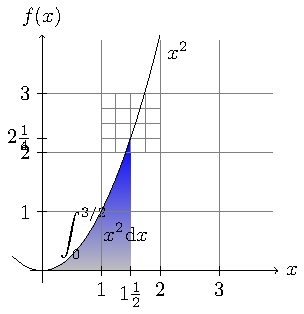
\includegraphics[width=0.7\linewidth]{mai_fig031.pdf}
    \caption{
            (\cite[s.~10000]{Feynman01})}
    \label{mai:fig031}
  \end{figure}

  \subsection{Výpočet integrálu}
      \begin{example}
        Spočítejme integrál $\displaystyle \int_1^{ln5}{(x+1)e^xdx}$  metodou per partes: 
        \begin{align*}
          \int{(x+1)e^xdx} &= \int{e^xdx}+\int{x\cdot e^xdx}
                            = e^x + (x-1)e^x = xe^x               \\
          \int_1^{ln5}{(x+1)e^xdx} &= [xe^x]_1^{ln5} = 5ln5-e     \\
        \end{align*}
        kde integrál
        \begin{equation*}
            \int{xe^xdx}=
              \left[\begin{array}{cc}
                u=x   & dv=e^x \\
                du=dx & v=e^x
              \end{array}\right]=
              xe^x-\int{e^xdx} = xe^x - e^x+C
        \end{equation*}
      \end{example}

\section{Vlastnosti určitého integrálu}
  V této kapitole mluvíme o spojitých funkcích $\Rightarrow$ příslušné integrály tedy vždy
  existují. Čerpáno z knih:
  \cite{Knichal}.

  \begin{lemma}
    \textbf{První věta o střední hodnotě integrálního počtu}: Je-li funkce $f(x)$ spojitá v
    intervalu $\langle a, b\rangle$, existuje alespoň jeden takový bod $c\in(a, b)$, že platí

    \begin{equation}\label{MA:eq_av1}
      \int_a^b f(x)dx = (b-a)f(c).
    \end{equation}
  \end{lemma}

  \begin{proof} Použitím Lagrangeovy věty napsané pro funkci $F(x)$, primitivní na intervalu
    $\langle a, b\rangle$ k dané funkci $f(x)$. Podmínky věty jsou zřejmě splněny: $F(x)$ je
    spojitá na intervalu $\langle a, b\rangle$ a má všude derivaci $F'(x)= f(x)$. Tedy existuje
    alespoň jeden bod $c\in(a, b)$,
    
    \begin{figure}[ht!]  %\ref{mai:fig029}
      \centering
      \includegraphics[width=0.7\linewidth]{mai_fig029.pdf}
      \caption{Vztah mezi silou tření a kolmou silou při smýkání
              (\cite[s.~173]{Feynman01})}
      \label{mai:fig029}
    \end{figure}

     že $$F(b)-F(a) = (b-a)F'(c),$$ čímž je věta dokázána, neboť $F(b)-F(a) = \int_a^bf(x)dx$ a
     $F'(c) = f(c)$. Funkční hodnotu $f(c)$, danou podle (\ref{MA:eq_av1}) rovnicí  
     \begin{equation}\label{MA:eq_av2}
        f(c) = \frac{1}{b-a}\int_a^b f(x)dx
     \end{equation}
     nazýváme \texttt{střední hodnotou}.
  \end{proof}

  Pro spojitou nezápornou funkci $f(x)$, lze větu o střední hodnotě jednoduše geometricky
  interpretovat dle (obr.\ref{mai:fig029}). Levá strana (\ref{MA:eq_av1}) určuje obsah
  křivočarého lichoběžníka $ABCD$, pravá strana obsah obdélníka $ABEF$. Podle této věty nabývá
  funkce $f(x)$ aspoň v jednom bodě intervalu $(a, b)$ takové hodnoty $f(c)$, že uvažovaný
  křivočarý lichoběžník má stejný obsah jako obdélník o základně $b-a$ a výšce $f(c)$ (str. 155
  knihy \cite{Knichal}).

      %---------------------------------------------------------------
      % !TeX spellcheck = cs_CZ
\begin{mdframed}[style=mdexam]
  \begin{example}\label{MAI:exam032}
    Určete střední hodnotu $i_s$ střídavého proudu $$i(t) = I_0\sin\omega t$$ v časovém intervalu
    $\langle 0, \frac{T}{2}\rangle$ (v průběhu jedné poloviny periody). $I_0$ je maximální hodnota
    proudu (obr. \ref{MAI:exam032}), perioda $T$ je dána vztahem $T = \frac{2\pi}{\omega}$
    
    {\centering
    \captionsetup{type=figure}
    \luafigure[1]{mai_fig030.pdf}
    \captionof{figure}{K příkladu \ref{MAI:exam032}
    \cite[s.~119]{Brabec1989}
    \label{mai:fig030}}
    \par}

      Podle \ref{MA:eq_av2} bude
      \begin{align*}
      i_s &=  \frac{2}{T}
              \int_0^{\frac{T}{2}}I_0\sin\omega t\dd{t} =
              \frac{2I_0}{T}\left[-\frac{\cos\omega t}{\omega}\right]_0^{\frac{T}{2}}        \\
          &=  \frac{2I_0}{T}\frac{1}{\omega}\left(-\cos\frac{\omega T}{2}+ \cos 0\right)     \\
          &=  \frac{2I_0}{2\pi}(-\cos\pi + \cos 0) = \frac{2}{\pi}I_0 \doteq 0,637 I_0.
    \end{align*}

    Tato hodnota se rovná intenzitě elektrického proudu, při kterém by vodičem v průběhu uvažované
    poloviny periody prošel stejný elektrický náboj jako při proudu střídavém.
  \end{example}
\end{mdframed}
















      %---------------------------------------------------------------

  \begin{example} Efektivní hodnota $i_{ef}$ střídavého proudu $$i(t) = I_0\sin\omega t$$ (viz
    předchozí příklad) je definována jako odmocnina ze střední hodnoty funkce $i^2(t)$ v průběhu
    jedné periody $T = \frac{2\pi}{\omega}$. Tedy
    \begin{align*}
      i_{ef}^2 &= \frac{1}{T}\int_0^T I_0^2\sin^2\omega t\dd{t} = 
                  \frac{1}{T}\int_0^T \frac{I_0^2}{2}(1- \cos2\omega t)\dd{t}           \\
               &= \frac{I_0^2}{2T}
                  \left[
                    t-\frac{\sin2\omega t}{2\omega}
                  \right]_0^T = \frac{I_0^2}{2}
    \end{align*}
    neboť $\sin2\omega T=\sin4\pi = 0.$ Odtud $$i_{ef} = \frac{I_0}{\sqrt{2}}.$$ Střídavý proud
    $i(t) = I_0\sin\omega t$ má na témže odporu stejný výkon jako stejnosměrný proud o intenzitě
    $i = 0,707I_0$.
  \end{example}
  Následující věta může být využita k odhadu některých integrálů
  \begin{lemma}
    \textbf{Druhá věta o střední hodnotě integrálního počtu}: Jsou-li funkce $f(x)$ a $g(x)$
    spojité v intervalu $\langle a, b \rangle$ a je-li funkce $g(x)$ v $\langle a, b \rangle$
    nezáporná a nerostoucí, existuje alespoň jeden bod $c\in\langle a, b \rangle$ tak, že platí
    \begin{equation}\label{MA_eq_av3}
        \int_a^b f(x)g(x) = g(a)\int_a^c f(x)dx.
    \end{equation}
  \end{lemma}
  Zcela obdobnou větu lze vyslovit pro případ, že $g(x)$ je v intervalu $\langle a, b \rangle$
  nezáporná a neklesající, tj. na pravé straně \ref{MA_eq_av3} je pak integrál $g(b)\int_c^b
  f(x)dx$

  \begin{example} Odhadněte hodnotu integrálu
    \begin{equation}\label{MA_eq_sinx_x}
        \int_{100\pi}^{1000\pi}\frac{\sin x}{x}dx
    \end{equation}
    Řešení: Funkce $f(x) = \sin x$ a $g(x) = \frac{1}{x}$ jsou v uvažovaném intervalu $\langle
    100\pi, 1000\pi \rangle$ spojité a funkce $g(x)$ je kladná a nerostoucí.
    \begin{equation*}
      \int_{100\pi}^{1000\pi}\frac{\sin x}{x}dx = 
      \frac{1}{100\pi}\int_{100\pi}^c\sin xdx =\frac{1}{100\pi}\left(\cos100\pi - \cos c\right)
    \end{equation*}
    kde $c$ je kladné číslo z intervalu $\langle 100\pi, 1000\pi \rangle$. Dále pro všechna
    $c\in\langle 100\pi, 1000\pi \rangle$ platí $0\leq1-\cos c\leq2$, takže
    \begin{equation*}
        0\leq\int_{100\pi}^{1000\pi}\frac{\sin x}{x}dx\leq \frac{1}{50\pi}.
    \end{equation*}
  \end{example}   

%} %tikzset
%---------------------------------------------------------------------------------------------------
\printbibliography[heading=subbibliography]
\addcontentsline{toc}{section}{Seznam literatury}
%---------------------Řady-------------------------------------------------------------------------
  % !TeX spellcheck = cs_CZ
%{\tikzset{external/prefix={tikz/MAI/}}
% \tikzset{external/figure name/.add={ch08_}{}}
%---------------------------------------------------------------------------------------------------
% file series.tex
%---------------------------------------------------------------------------------------------------
%==================================== Kapitola: Řady================================================
\chapter{Řady}
\minitoc

%} % tikzset
%---------------------------------------------------------------------------------------------------
%\printbibliography[title={Seznam literatury}, heading=subbibliography]
\addcontentsline{toc}{section}{Seznam literatury}  
%---------------------Obyčejné diferenciální rovnice ----------------------------------------------
  % !TeX spellcheck = cs_CZ
%{\tikzset{external/prefix={tikz/MAI/}}
% \tikzset{external/figure name/.add={ch09_}{}}
%---------------------------------------------------------------------------------------------------
% file ODR.tex
%---------------------------------------------------------------------------------------------------
\chapter{Obyčejné diferenciální rovnice}
\minitoc
%================Kapitola: Diferenciální rovnice 1. řádu ===========================================
  \section{Diferenciální rovnice 1. řádu}
    Řada fyzikálních principů má tvar výroku, resp. vztahu mezi jistými veličinami (funkcemi) a
    jejich změnami, vztaženými ke zvoleným nezávisle proměnným pa\-ra\-me\-trům (čas, souřadnice).
    Změny (okamžité, lokální) se nejlépe vystihují pomocí derivací. Takový zákon má pak charakter
    vztahu mezi uvažovanými veličinami a jejich derivacemi. Nejčastěji bývá vztah vyjádřen formou
    rovnosti:
    \begin{itemize}
   	  \item Newtonůw zákon: okamžitá změna hybnosti $p(t) = m(t)\cdot v(t)$ pohybujícího se
         	objektu je úměrná působící síle $F(t)$ v každém okamžiku $t$ zvoleného časového rozmezí
        	$$\frac{d}{dt}\left(m(t)\cdot v(t)\right) = F(t)\quad t\in\langle\alpha, \beta\rangle$$
      \item Kirchhoffův zákon pro LR – obvod: v okamžiku $t$ je součet napětí na cívce s indukčnosti
            $L$ a na rezistoru o odporu $R$ roven napětí $U(t)$ na svorkách zdroje. Tuto rovnost pak
            zapisujeme ve tvaru (pro L,R = konst)
            \begin{equation}
              L\frac{di(t)}{dt}+Ri=u(t), 
            \end{equation}
            kde $i=i(t)\ldots$ funkce popisující závislost proudu na čase.
    \end{itemize}
    
    Chceme-li určit funkci $i=i(t)$ popisující průběh proudu v obvodu tak, aby byl splněn příslušný
    K.z. a současně, aby byl splněn požadavek na počáteční stav:
    \begin{equation}
        L\frac{di(t)}{dt}+Ri(t)=U,\quad i(0)=I_0,\quad t\in\langle 0,+\infty)
    \end{equation}
    Metodami uvedenými později stanovíme právě jednu funkci $i=i(t)$, která je řešením dané tzv.
    \textbf{počáteční úlohy}.
    \begin{equation}
      \begin{array}{c}
         i(t)=I_0\left(1-e^{-\frac{R}{L}t}\right),\quad t\in\langle 0,+\infty), \\
         lim_{t\rightarrow +\infty}i(t)=\frac{U_0}{R},\quad lim_{t\rightarrow +0}i(t)=I_0=i(0)
      \end{array}
    \end{equation}
    \begin{itemize}
      \item tedy obvykle formulujeme úlohu najít jistou funkci tak, aby zákon byl splněn tj.
            Kirchhoffův zákon užijeme k tomu, abychom nalezli funkci $i(t)$
      \item užijeme-li rovnosti vyjadřující takový zákon k tomu, abychom určili funkci, která v
            takovém vztahu vystupuje spolu s derivacemi, stává se tento požadavek úlohou, která má
            charakter rovnice s derivacemi, neboli diferenciální rovnice. Funkce, která požadavek
            splňuje, se pak nazývá řešení diferenciální rovnice.
    \end{itemize}
    
    \begin{figure}
      \centering
      \includegraphics[width=\linewidth]{mai_fig032.pdf}
      \caption{Graf průběhu proudu $i(t)$ po sepnutí spínače v době $t=0$.}
      \label{mai:fig032}
    \end{figure}

%} %tikzset
%---------------------------------------------------------------------------------------------------
%\printbibliography[heading=subbibliography]
\addcontentsline{toc}{section}{Seznam literatury}
%---------------------Numerické metody ------------------------------------------------------------
  % !TeX spellcheck = cs_CZ
%{\tikzset{external/prefix={tikz/MAI/}}
% \tikzset{external/figure name/.add={ch10_}{}}
%---------------------------------------------------------------------------------------------------
% file ppst.tex
%---------------------------------------------------------------------------------------------------
\chapter{Počet Pravděpodobnosti}
\minitoc
  Slovo pravděpodobnost používáme velmi často. Jaký však je jeho přesný význam? Jsme přesvědčeni, 
  že pravděpodobnost výhry ve sportce je velmi malá. Ani pravděpodobnost, že se vyplní předpověď 
  počasí, nepovažujeme mnohdy za výraznou. Přesto je mezi oběma příklady obrovský kvantitativní 
  rozdíl. Zkusme význam pojmu pravděpodobnost ukázat pomocí konkrétních číselných příkladů.
  
  \begin{itemize}
    \item \textbf{Příklad se střelcem}: Sportovní střelec střílí na terč série \num{100} ran. 
          Předpokládejme, že podmínky při střelbě jsou stále stejné. Stejná je zbraň, terč, 
          vzdálenost, povětrnostní podmínky i momentální zdravotní stav střelce. Při hodnocení 
          střelcova „mistrovství“ někdo řekne, že střelec zasáhne terč s pravděpodobností 
          \num{92}\%. Jak tomu rozumět? Znamená to, že v souboru sérií výstřelů jsou velmi časté 
          ty, v nichž zasáhl střelec terč \num{92}-krát. Samozřejmě, není řídké, že se objeví i 
          série s \num{93} nebo \num{94} zásahy, ale také s \num{91} nebo \num{90}. Vyloučen není 
          ani případ s úspěšností \num{96} či \num{88}, a dokonce i stovku bychom mohli zaznamenat. 
          Situace výrazně odlišné od \num{92} zásahů však budou řídké, a to tím více, čím více se 
          úspěšnost série liší od \num{92} oběma směry.
    \item \textbf{Příklad se zmetky}: Koupíte si výrobek u firmy, o které je známo, že vyrábí 
          zmetky s pravděpodobností 0,16\%? Situaci lze posuzovat obdobně jako úspěšnost střelce. 
          Budeme-li například zkoumat série obsahující 1000 výrobků, bude každá z nich obsahovat „v 
          průměru“ 16\% zmetků. Z příkladu se střelcem již zhruba víme, jak posuzovat slovo v 
          průměru.
  \end{itemize}
  
  V této kapitole se budeme pravděpodobnostmi zabývat podrobněji. Zjistíme, že i když se týkají 
  náhodných jevů, platí i pro ně jisté zákonitosti.
    
  \section{Pravděpodobnost}
    V úvodních příkladech jsme si vyložili, jak intuitivně chápat pojem pravděpodobnost. Jednalo se 
    v nich o posouzení průměrné úspěšnosti ve velkém souboru operací či úkonů prováděných za 
    stejných podmínek, šlo tedy o jakousi „průměrnou“ pravděpodobnost. Nyní definujeme 
    pravděpodobnost matematicky.
    
    \subsection{Co se pravdě podobá — definice pravděpodobnosti}
      Pro definici pravděpodobnosti použijeme pojmu \emph{náhodný pokus}, jehož význam si ukážeme 
      na příkladu. Dobrým příkladem náhodných pokusů je třeba házení mincí, hraní kostkou, výběr 
      karet z balíčku, vidíme-li pouze jejich rub, apod. Budeme třeba házet kostkou. Abychom si 
      situaci zbytečně nekomplikovali, budeme předpokládat, že všechny výsledky hodu kostkou 
      (náhodné pokusy) jsou stejně časté, žádný z nich není nijak preferován\footnote{Kostka by 
      tedy měla být homogenní, plocha, na kterou po hodu dopadne, vodorovná, kvalita povrchu všech 
      stěn kostky stejná (žádná stěna by třeba neměla být natřena lepidlem), apod.}. Počet možných 
      výsledků jednotlivého hodu je \(N = 6\) (kostka má \num{6} stěn, na každé je vyznačen odlišný 
      počet ok, tedy \num{1} až \num{6}). Jednotlivé situace, které mohou nastat, nazýváme 
      náhodnými jevy. Náhodným jevem \(A\) tak může být situace \emph{„padne číslo \num{2}“}, jiným 
      náhodným jevem \(B\) situace \emph{„padne číslo dělitelné třemi“}, apod. Počet situací, kdy 
      výsledek hodu lze hodnotit tak, že určitý jev nastal, označíme \(M\). Například pro jev \(A\) 
      \emph{„padne číslo \num{2}“} je \(M(A)= 1\), pro jev \(B\) \emph{„padne číslo dělitelné 
      třemi“} je \(M(B) = 2\) (počet ok \num{3} nebo \num{6}). Můžeme také definovat jev \(O\) 
      \emph{„nepadne žádné číslo“} (\(M(0) = 0\)) nebo jev \(J\) \emph{„padne jakékoli číslo“} 
      (\(M(J) = 6\)).
      
      \begin{definition}
        Pravděpodobností jevu rozumíme podíl
        \begin{equation}\label{mai:eq011}
          p = \frac{M}{N} = \frac{\text{počet případů příznivých}}{\text{počet případů možných}}.
        \end{equation}  
        Počtem případů možných jsme zkráceně nazvali počet všech možných výsledků náhodného 
        pokusu, počtem případů příznivých pak počet všech takových výsledků pokusu, při nichž daný 
        jev nastal.
      \end{definition}
      Je zřejmé, že hodnota pravděpodobnosti jakéhokoli jevu je nezáporná a může nabývat hodnoty 
      nejvýše \num{1}, tj. \(0 <p< 1\). Jev s \emph{nulovou pravděpodobností} se nazývá 
      \textbf{nemožný}, jev s \emph{jednotkovou pravděpodobností} je \textbf{jistý}. V našem 
      příkladu s kostkou tak dostáváme
      \begin{equation*}
        p(A) = \frac{1}{6}, \qquad p(B) = \frac{2}{6} = \frac{1}{3}, \qquad
        p(O) = 0, \qquad p(J) = 1.
      \end{equation*}  

      %---------------------------------------------------------------
      % !TeX spellcheck = cs_CZ
\begin{example}
 \label{mai:exam006}
  \textbf{Barevné ponožky}:\newline\small
  V zásuvce jsou ponožky tří barev. Červené (\textbf{Č}), zelené (\textbf{Z}) a modré (\textbf{M}). 
  Je jich tam od každé barvy hodně. Student jde na schůzku a chce si vzít čisté ponožky. Náhle 
  zhasne světlo. Student vytáhne potmě dvě ponožky. Jaká je pravděpodobnost, že ponožky budou mít 
  stejnou barvu? Vyjmenujme případy, které mohou při vytažení dvou ponožek nastat: (\textbf{Č+Č}), 
  (\textbf{Č+Z}), (\textbf{Z+Č}), (\textbf{Č+M}), (\textbf{M+Č}), (\textbf{Z+Z}), (\textbf{Z+M}), 
  (\textbf{M+Z}), (\textbf{M+M}). Je tedy \(n = 9\). Příznivé situace jsou tří, (\textbf{Č+Č}), 
  (\textbf{Z+Z}), (\textbf{M+M}). Pravděpodobnost je tedy 1/3. (Převzato z 
  \cite[s.~200]{Musilova2009MA1}) 
\normalsize
\end{example}
      %---------------------------------------------------------------
    \subsection{Cifry, kostky, karty - kombinatorické opakování}
      Příklad s ponožkami byl velmi jednoduchý. Podařilo se nám vyjmenovat všechny případy možné i 
      všechny případy příznivé, neboť obojího bylo docela málo. Daleko běžnější jsou však situace, 
      kdy výčet případů není schůdný. A tehdy potřebujeme \textbf{kombinatoriku}.
      
      Nechť \(\mathcal{M}\) je \(n\)-prvková množina, z níž budeme provádět výběry \(k\) prvků 
      podle určitých pravidel. Prvky množiny \(\mathcal{M}\) nemusíme nijak konkretizovat. Abychom 
      si však o výběrech a pravidlech pro jejich tvorbu dokázali udělat nějakou názornou představu, 
      je taková konkretizace vhodná. Prvky množiny \(\mathcal{M}\): mohou být třeba žáci ve třídě, 
      barvy, hrací karty, apod. Výběry mohou představovat třeba družstva pro odbíjenou, signály 
      tvořené barevnými praporky, možnosti rozdání karet při mariáši, apod. Jednotlivé typy výběrů 
      získaly své názvy právě na základě pravidel stanovených pro jejich vytváření. Rozhodující 
      jsou dvě základní kritéria:
      \begin{itemize}\addtolength{\itemsep}{-0.5\baselineskip}
        \item Je pro tvorbu výběru podstatné pořadí prvků ve výběru či nikoliv?
        \item Mohou se prvky ve výběru opakovat či nikoliv?
      \end{itemize}
      
      Typy výběrů shrnuje následující diagram:
      \begin{figure}[ht!] %\ref{mai_fig021}
        \centering
        \includegraphics[width=0.7\linewidth]{mai_fig021.pdf}
        \caption{Typy výběrů. \cite[s.~201]{Musilova2009MA1}}
        \label{mai_fig021}
      \end{figure}

      Představuje-li daný výběr například volejbalové družstvo osmi děvčat (šest hráček a dvě 
      náhradnice), které bude reprezentovat v soutěži třídu osmou bé, do níž chodí \num{25} děvčat 
      a \num{18} chlapců, jedná se o výběr \(k — 8\) prvků z počtu \(n = 25\) prvků. Chlapce nelze 
      postavit do družstva volejbalistek. Každý výběr možného družstva bude představovat 
      \emph{kombinaci bez opakování}, neboť pořadí hráček nehraje roli a třeba Aničku Novákovou 
      máme ve třídě jen jednu. Budeme-li však chtít vytvářet z deseti cifer \(0, 1, \ldots, 9\) 
      trojciferná čísla, pak tyto výběry tří prvků z deseti (\(k = 3\), \(n = 10\)) jsou 
      \emph{variacemi s opakováním}. Čísla \num{125}, \num{512}, \num{251}, \num{215}, \num{521} a 
      \num{152} jsou totiž různá, a například \num{222} je také trojciferné číslo. Kombinace s 
      opakováním bychom mohli vytvářet třeba i při výběru různobarevných ponožek ze zásuvky a 
      konečně \emph{variacemi bez opakování} by mohly být dejme tomu trojbarevné signály (\(k = 
      3\)) tvořené trojicemi barevných hadříků vybíraných z \(n\) barev (pro \(n = 3\) třeba zrovna 
      z těch ponožek). Nyní bychom však rádi věděli, jak pro zadané hodnoty \(n\) a \(k\) určit 
      počet všech možných výběrů předepsaného typu. Ukážeme si to na příkladech.

      %---------------------------------------------------------------
      % !TeX spellcheck = cs_CZ
\begin{mdframed}[style=mdexam]
  \begin{example}\label{mai:exam007}
    \textbf{Šance milion}:\newline
    „Znáte nějakou jinou hru, kde můžete denně vyhrát milion?“ Tento nebo jiný, obdobně nepříliš
    vtipný reklamní slogan propaguje v televizi hru, jejímž cílem je uhodnout šestici tažených cifer
    ve správném pořadí. (Hru raději nehrajte, pravděpodobnost výhry je mizivá.) Tah se provádí
    následovně: V každém ze šesti bubnů, očíslovaných pořadovými čísly \num{1} až \num{6}, je
    připraveno deset míčků opatřených ciframi \(0, 1, \ldots, 9\). Z prvního bubnu se náhodně
    vylosuje jedna cifra (deset možností). Poté se náhodně vylosuje jedna cifra z druhého bubnu
    (opět deset možností). Možností vzniku uspořádané dvojice cifer (jedna cifra z prvního a druhá z
    druhého bubnu) je již sto (každou možnost výsledku u prvního bubnu lze kombinovat s každou
    možností výsledku z druhého bubnu). Losování pokračuje u třetího, čtvrtého, pátého a šestého
    bubnu. Celkový počet možností je \num{1e6}, tedy \textbf{milion}. (Šance získat výhru, tedy
    vyhrát milion, je ovšem pouze jedna milióntina, neboť z milionu možností je pouze jedna skutečně
    tažena.) 
  \end{example}
\end{mdframed}
      %---------------------------------------------------------------
      
      Zobecněním předchozího příkladu získáváme vzorec pro počet \textbf{variací s opakováním} 
      \emph{k}-té třídy z \(n\) prvků. Při tahu totiž záleží na pořadí bubnů a každý buben obsahuje 
      všechny cifry. Výsledky tahů z jednotlivých bubnů se tedy mohou opakovat. Pokud by bubnů bylo 
      \(k\) a v každém \(n\) různých cifer, dostali bychom pro \textbf{variace s opakováním 
      \(k\)-té třídy z \(n\) prvků} celkový počet
      \begin{equation}\label{mai:eq007}
        \boxed{V_k' = n^k}\, .
      \end{equation}

      %---------------------------------------------------------------
      % !TeX spellcheck = cs_CZ
\begin{example}\label{mai:exam008}
  \textbf{Modifikovaná šance milion}:\newline
  Představme si hru z předchozího příkladu upravenou takto: K dispozici bude jen jeden buben s 
  ciframi \(0, 1, \ldots, 9\), každá cifra je v bubnu obsažena pouze jednou. Opět máme losovat 
  uspořádanou \textbf{šestici cifer}. Nyní se však jedná o \textbf{variace šesté třídy z deseti 
  prvků bez opakování}. S jediným bubnem musíme totiž provést šest losování, přičemž při každém 
  losování ubude z bubnu jedna cifra. Při prvním tahu je deset možností, při druhém již jen devět, 
  atd., při šestém již pouze pět možností. Celkem je tedy \(10 \cdot 9 \cdots 5 = \num{151200}\) 
  možností.
\end{example}
      %---------------------------------------------------------------
      
      Uvážíme-li, že v předchozím příkladu je \(n = 10\) a \(k = 6\), dostáváme pro \textbf{počet 
      variací bez opakování \(k\)-té třídy z \(n\) prvků} obecný vztah
      \begin{align}
        V_k(n) &= n(n-1)(n-2)\cdots(n-k+1)  \nonumber \\
        \shortintertext{neboli}
        V_k(n) &= \frac{n!}{(n-k)!}\, .    \label{mai:eq008}
      \end{align}
      Poznamenejme, že \(n!\) značí \textbf{faktoriál}, \(n! = n(n — 1)\cdots 3 \cdot 2 \cdot 1\). 
      Pro nulu definujeme \(0! = 1\). Je zřejmé, že při vytváření variací bez opakování musí být 
      \(k\leqq n\). Variace bez opakování \(n\)-té třídy z \(n\) prvků se nazývají 
      \textbf{permutace}. Každá z nich představuje určité uspořádání těchto \(n\) prvků. Platí
      \begin{equation}\label{mai:eq009}
        \boxed{P(n) = V_n(n) = n!}\, .
      \end{equation}
      
      Nyní odvodíme vzorec pro počet \textbf{kombinací \(k\)-té třídy z \(n\) prvků bez opakování}. 
      Již jsme si řekli, že \emph{kombinací} rozumíme takový výběr z celkového počtu \(n\) prvků, 
      který obsahuje určitých \(k\) prvků nezávisle na jejich pořadí. Představme si, že máme k 
      dispozici všechny variace bez opakování \(k\)-té třídy ze zmíněných \(n\) prvků. Vezměme 
      kteroukoli z nich. Soubor všech variací \(k\)-té třídy z \(n\) prvků však obsahuje i další 
      variace, lišící se od té naší jen pořadím prvků. Celkem je takových variací (i s tou první) 
      \(k!\) a z hlediska kombinací představují totéž. Soubor variací se tak rozpadá na podsoubory, 
      z nichž každý obsahuje \(k!\) variací lišících se navzájem pouze pořadím prvků. Každý z 
      těchto podsouborů představuje však jedinou kombinaci. Počet kombinací \(k\)-té třídy z \(n\) 
      prvků bez opakování je tedy
      \begin{equation}\label{mai:eq010}
        \boxed{C(k) = \frac{V_k(n)}{P(k)} = \frac{n!}{(n-k)!\,k!} = 
               \begin{pmatrix}
                n \\
                k
               \end{pmatrix}}\, .
      \end{equation}
      
      Pro odvození vzorce pro \textbf{kombinace s opakováním} použijeme opět příkladu.
      %---------------------------------------------------------------
      % !TeX spellcheck = cs_CZ
\begin{mathexam}{Kuličky v přihrádkách}{exam009}
  Máme kuličky \(n\) různých barev, v každé barvě máme tolik kuliček, kolik bude potřeba. Naším
  úkolem je vytvářet výběry \(k\) kuliček. Na \textbf{pořadí barev nezáleží}, kuliček jedné barvy
  může být ve výběru libovolný počet \(0\leqq s \leqq k\). Výběry budeme vytvářet tak, že budeme
  kuličky dávat do \(n\) přihrádek, z nichž každá bude vyhrazena pro určitou barvu. Pokud tedy v
  daném výběru zrovna nebude třeba modrá kulička, bude přihrádka vyhrazená pro modrou barvu prázdná.
  Budou-li v daném výběru právě tři červené kuličky, budou umístěny v přihrádce vyhrazené pro
  červenou barvu. Vidíme, že pokud konkrétním přihrádkám přisoudíme konkrétní barvy, samotné kuličky
  by již barevné být nemusely, stačily by třeba kuličky skleněné, bezbarvé. Zůstane-li například
  přihrádka pro modrou barvu prázdná, víme, že daný výběr neobsahuje modrou barvu. Budou-li v
  přihrádce pro červenou barvu tři (bezbarvé) kuličky, víme, že daný výběr obsahuje červenou barvu
  třikrát. Příklad takové situace ukazuje následující schéma:
  
  {\centering
    \luafigure[0.9]{mai_fig033.pdf}
    \par}

  Náš úkol můžeme přeformulovat takto: Je třeba rozmístit \(k\) kuliček do \(n\) přihrádek. V každé
  přihrádce může být obecně \(s\) kuliček, kde \(0\leqq s \leqq k\), přitom celkový počet kuliček
  musí být samozřejmě stále \(k\). Můžeme si představit, že \(k\) kuliček máme položených v řadě na
  polici mezi dvěma pevnými stěnami (krajní svislé čáry v předchozím schématu) a různé způsoby
  rozmístění kuliček do přihrádek provádíme přemísťováním pohyblivých přepážek. Kdybychom například
  v předchozím schématu přesunuli druhou svislou čáru, počítáno zleva, až za první kuličku v
  přihrádce na červenou barvu, dostaneme uspořádání, při němž je v přihrádce na modrou barvu jedna
  kulička a v přihrádce na červenou barvu dvě kuličky. Tedy takto:

  {\centering
    \luafigure[0.9]{mai_fig034.pdf}
  \par}

  Mezi dvěma krajními pevnými stěnami máme tedy k dispozici \(k\) pozic pro kuličky a \((n - 1)\)
  pozic pro pohyblivé přepážky. Celkem tedy \((n + k - 1)\) pozic, na které můžeme libovolně
  rozmísťovat \(k\) kuliček a \((n - 1)\) přepážek. Do těchto \((n + k - 1)\) pozic můžeme umístit
  \(k\) kuliček \(C_k'(n)\) způsoby, kde
  \begin{equation}\label{MAI:eq011}
    \boxed{C_k'(n) =  \binom{n + k - 1}{k} = \binom{n + k - 1}{n -1}}\, .
  \end{equation}
  Na zbylé pozice již musíme umístit přepážky. Nebo naopak, nejprve umístíme \((n - 1)\) přepážek a
  potom kuličky. Výsledek je stejný, jak je vidět z předchozího vzorce. Protože jsme vytváření
  kombinací s opakováním \(k\)-té třídy z \(n\) prvků převedli na úlohu o rozmísťování kuliček do
  přihrádek, udává získaný vzorec právě počet takových kombinací. Aby měl vzorec smysl, musí platit
  \(n + k - 1 \geqq k\), tedy \(n \geqq 1\).

  Komu nevyhovuje představa kuliček v přihrádkách a má raději čísla, může uvažovat následovně: Tak
  jako je každé číslo v desítkové soustavě zapsáno pomocí cifer \(0, 1, 2, \ldots , 8, 9\), je k
  jeho zápisu ve dvojkové soustavě potřeba pouze dvou cifer, nuly a jedničky. Představme si nyní
  přepážku jako jedničku a kuličku jako nulu. Náš úkol zjistit počet všech možných způsobů rozdělení
  \(k\) kuliček do \(n\) přihrádek, ohraničených \((n+1)\) přepážkami, můžeme převést na
  ekvivalentní problém: Kolik dokážeme najít čísel, která jsou ve dvojkové soustavě zapsána právě
  \(k\) nulami a \((n + 1)\) jedničkami, požadujeme-li, aby první i poslední cifrou byla jednička?
  Odpověď je jednoduchá. Máme k dispozici \((n+k+1)\) pozic pro cifry. První a poslední pozice jsou
  pevně obsazeny jedničkami, volných pozic je tedy pouze \((n + k - 1)\). Počet všech různých
  způsobů, kterými na \(k\) z těchto pozic můžeme umístit nuly, je roven počtu kombinací \(k\)-té
  třídy z \((n + k - 1)\) prvků. Na zbylé pozice již musíme umístit jedničky. Komplementárně,
  budeme-li hledat počet všech možných způsobů, jak na \((n-1)\) pozic umístit jedničky, dostaneme
  shodný výsledek, v souhlasu se vzorcem (\ref{mai:eq010}).
\end{mathexam}
      %---------------------------------------------------------------
      
      Komu nevyhovuje představa kuliček v přihrádkách a má raději čísla, může uvažovat následovně: 
      Tak jako je každé číslo v desítkové soustavě zapsáno pomocí cifer \(0, 1, 2, \ldots , 8, 9\), 
      je k jeho zápisu ve dvojkové soustavě potřeba pouze dvou cifer, nuly a jedničky. Představme 
      si nyní přepážku jako jedničku a kuličku jako nulu. Náš úkol zjistit počet všech možných 
      způsobů rozdělení \(k\) kuliček do \(n\) přihrádek, ohraničených \((n+1)\) přepážkami, můžeme 
      převést na ekvivalentní problém: Kolik dokážeme najít čísel, která jsou ve dvojkové soustavě 
      zapsána právě \(k\) nulami a \((n + 1)\) jedničkami, požadujeme-li, aby první i poslední 
      cifrou byla jednička? Odpověď je jednoduchá. Máme k dispozici \((n+k+1)\) pozic pro cifry. 
      První a poslední pozice jsou pevně obsazeny jedničkami, volných pozic je tedy pouze \((n + k 
      — 1)\). Počet všech různých způsobů, kterými na \(k\) z těchto pozic můžeme umístit nuly, je 
      roven počtu kombinací \(k\)-té třídy z \((n + k — 1)\) prvků. Na zbylé pozice již musíme 
      umístit jedničky. Komplementárně, budeme-li hledat počet všech možných způsobů, jak na 
      \((n—1)\) pozic umístit jedničky, dostaneme shodný výsledek, v souhlasu se vzorcem 
      (\ref{mai:eq010}).
      
      %---------------------------------------------------------------
      % !TeX spellcheck = cs_CZ
\begin{example}\label{mai:exam010}
  \textbf{Obsazování kvantových stavů}:\newline\small
  Úloha o kuličkách a přihrádkách má přímou aplikaci v \textbf{kvantové fyzice}. Představme si, že 
  fyzikální soustava je tvořena \(k\) částicemi. Každá částice se nachází v určitém stavu, v němž 
  jí můžeme přisoudit fyzikální charakteristiky, které jsou s tímto stavem spojeny (třeba energii, 
  moment hybnosti, apod.). Jednotlivé stavy jsou pak rozlišitelné právě pomocí těchto 
  charakteristik. Dejme tomu, že přípustných stavů je \(n \geqq 1\). Problémem kvantové fyziky je 
  to, že kvantové částice jsou nerozlišitelné. Nepoznáme jednu od druhé. Je to stejné, jako bychom 
  měli \(k\) naprosto stejně vypadajících kuliček, které nemáme nijak očíslovány. Záměna dvou 
  částic (nerozlišitelných kuliček) se nepozná, nevede tedy ke změně stavu fyzikální soustavy. Pro 
  hodnoty fyzikálních charakteristik soustavy jako celku je tedy důležité jen to, kolik částic je v 
  každém z přípustných stavů. Musíme se tedy zajímat o to, kolika způsoby lze našich \(k\) 
  \textbf{nerozlišitelných částic} (kuliček) umístit do \(n\) \textbf{stavů} (přihrádek). Kvantové 
  částice jsou však dvojího druhu, \textbf{fermiony} (například elektrony, neutrony, protony, jádra 
  s lichým počtem nukleonů) a \textbf{bosony} (například fotony, mezony, jádra se sudým počtem 
  nukleonů). Rozdíl mezi nimi je ten, že bosony se „dobře snášejí“, a proto jich může být v jednom 
  stavu i více. 
  \begin{itemize}\addtolength{\itemsep}{-0.5\baselineskip}
    \item Počet možností, jak rozmístit \(k\) \textbf{bosonů} po \(n\) stavech je tedy
          \begin{equation*}
            N_{\text{boson}} = 
              \begin{pmatrix}
                n + k - 1 \\
                    k
               \end{pmatrix}
          \end{equation*}
    \item S \textbf{fermiony} je tomu jinak. \textbf{Pauliho vylučovací princip} jim zakazuje, 
          aby v daném stavu byl více než jeden fermion. Stav může být buď prázdný, nebo obsazen 
          jedním fermionem. V takovém případě musí být \(n \geqq k\) a v každé přihrádce může být 
          nejvýše jedna kulička. Situace tak odpovídá \textbf{kombinacím bez opakování \(k\)-té 
          třídy z \(n\) prvků}, tj.
          \begin{equation*}
            N_{\text{fermion}} = 
              \begin{pmatrix}
                n  \\
                k
              \end{pmatrix}
          \end{equation*}
  \end{itemize}
\normalsize
\end{example}
      %---------------------------------------------------------------
      
      Získané kombinatorické vzorce nyní použijeme při řešení základních úloh o pravděpodobnostech. 
      V každé úloze bude důležité
      \begin{itemize}
        \item definovat jev \(A\), jehož pravděpodobnost počítáme,
        \item určit počet \(N\) případů možných, tj. počet všech možných výsledků pokusu, při 
              kterém sledujeme, zda jev \(A\) nastal či nenastal,
        \item určit počet \(M\) případů příznivých, tj. počet těch výsledků daného pokusu, při 
              kterých jev \(A\) nastal.
      \end{itemize}

      %---------------------------------------------------------------
      % !TeX spellcheck = cs_CZ
\wikitextrule
\begin{example}\label{mai:exam052}
  \textbf{Výhra ve sportce}\newline\small
  Jaká je pravděpodobnost hlavní výhry ve sportce? Všichni víme, že malá, ale máme představu, jak 
  malé toto číslo je? Při sportce se losuje \(k = 6\) čísel a jedno dodatkové z celkového počtu \(n 
  = 49\) čísel. (Dříve byla čísla spojena s názvy sportů, odtud název „sportka“ .) Na pořadí čísel 
  ve výběru nezáleží, vytažené číslo se do hry nevrací. Jde tedy o \textbf{kombinace bez 
  opakování}. Hlavní výhra požaduje uhodnout všech \num{6} tažených čísel. Jev \(A\) je tedy 
  definován takto:
  
  \begin{itemize}
    \item Jev \(A\): Bude taženo právě oněch \num{6} čísel, která jsem vsadil.
          Počet možností, které při tahu sportky mohou nastat (počet případů možných), je \(N = 
          \begin{pmatrix} n \\ k\end{pmatrix} =  \begin{pmatrix} 49 \\ 6 \end{pmatrix} \). Hlavní 
          výhru představuje jediná kombinace, počet příznivých případů je proto \(M = 1\). 
          Pravděpodobnost hlavní výhry ve sportce, tj. pravděpodobnost jevu \(A\), je
          \begin{equation*}
            p(A) = \dfrac{M}{N} = \dfrac{1}{\begin{pmatrix} 49 \\ 6 \end{pmatrix}} 
                 = \dfrac{43!6!}{49!} = \dfrac{720}{49\cdot48\cdot47\cdot46\cdot45\cdot44} \simeq 
                 \num{7e-8}
                 = \SI{7e-6}{\percent}
          \end{equation*}
          Pravděpodobnost hlavní výhry je velmi malá, sedm milióntin procenta. 
    \item A o kolik lepší to bude s pravděpodobností některé z vedlejších výher? Tak třeba pátá 
          cena znamená, že je nutné ze šesti tažených čísel uhodnout libovolné tři. Jev \(A\) je 
          tedy: Ze šesti čísel, která jsme vsadili, budou v tažené kombinaci obsažena právě tři 
          libovolná z nich. Počet \(N\) zůstává stejný jako v předchozí části úlohy. Je třeba jen 
          určit \(M\). Každý příznivý případ vzniká tak, že trojice správných čísel (výběry tří ze 
          šesti) je doplněna trojicí chybných čísel (výběry tří ze čtyřiceti tří). Tedy \(M = 
          \begin{pmatrix}6 \\ 3\end{pmatrix}\begin{pmatrix} 49 - 6 \\ 3\end{pmatrix} =  
          \begin{pmatrix} 6 \\ 3\end{pmatrix}\begin{pmatrix} 43 \\ 3 \end{pmatrix}\),
          \begin{align*}
            p(A) &= \dfrac{M}{N} 
                  = \dfrac{\begin{pmatrix} 6 \\ 3\end{pmatrix}
                           \begin{pmatrix} 43 \\ 3 \end{pmatrix}}
                          {\begin{pmatrix} 49 \\ 6\end{pmatrix} }                
                  =\left(\dfrac{6!}{3!\cdot3!}\right)\left(\dfrac{43!}{40!\cdot3!}\right)
                   \left(\dfrac{43!6!}{49!}\right)                                            \\
                 &=\dfrac{120\cdot43\cdot42\cdot41\cdot720}
                         {49\cdot48\cdot47\cdot46\cdot45\cdot44\cdot36} 
                  \simeq\num{0.018}.
          \end{align*}
          Tato pravděpodobnost již zanedbatelná není, na rozdíl od finanční částky, jíž bývá 
          ohodnocena pátá cena. Sázení sportky může domácímu rozpočtu spíše ublížit.
    \item Třetí, resp. čtvrtá cena jsou, podobně jako první a pátá, definovány velmi jednoduše. Je 
          třeba uhodnout pět, resp. čtyři ze šesti tažených čísel. V případě druhé ceny hraje roli
          dodatkové číslo. Druhou cenu získává ten, kdo uhodl pět ze šesti čísel vylosovaných v 
          prvním tahu a ještě navíc číslo dodatkové, které se losuje ze zbylých \num{43} čísel, jež 
          zůstala po prvním tahu v osudí. Jev \(A\) je tedy definován takto:
          
          Ze šesti čísel, která jsem vsadil, bude při prvním tahu vylosováno libovolných pět a v 
          druhém tahu bude vylosováno právě to dodatkové číslo, které jsem vsadil. Počet případů 
          příznivých je pouze \(M = \begin{pmatrix}6 \\ 5\end{pmatrix}\), neboť šestým číslem 
          nemůže být libovolné ze \num{43} čísel, která nebyla v prvním tahu vylosována, ale 
          musí to být právě číslo dodatkové. Pravděpodobnost jevu \(A\) je
          \begin{equation*}
            p(A)  = \dfrac{M}{N} 
                  = \dfrac{\begin{pmatrix} 6  \\ 5\end{pmatrix}}
                          {\begin{pmatrix} 49 \\ 6\end{pmatrix}}
                  \simeq\num{4.2e-17}.
          \end{equation*}
          
          Pokud bychom jako jev \(A\) označili výhru jakékoliv ceny, dostaneme
          \begin{align*}
            M &= \sum_{6}^{k=3}\begin{pmatrix} 6  \\   k  \end{pmatrix}
                               \begin{pmatrix} 43 \\ 6 - k\end{pmatrix}  +
                               \begin{pmatrix} 6  \\   5  \end{pmatrix}                      \\
              &= \begin{pmatrix} 6 \\ 3\end{pmatrix}\begin{pmatrix} 43 \\ 3\end{pmatrix} +
                 \begin{pmatrix} 6 \\ 4\end{pmatrix}\begin{pmatrix} 43 \\ 2\end{pmatrix} +
                 \begin{pmatrix} 6 \\ 5\end{pmatrix}\begin{pmatrix} 43 \\ 1\end{pmatrix} +
                 \begin{pmatrix} 6 \\ 6\end{pmatrix}\begin{pmatrix} 43 \\ 0\end{pmatrix} +
                 \begin{pmatrix} 6 \\ 5\end{pmatrix},                                        \\
           p(A) &= \dfrac{\begin{pmatrix}  6 \\ 3\end{pmatrix}
                          \begin{pmatrix} 43 \\ 3\end{pmatrix}  +
                          \begin{pmatrix}  6 \\ 4\end{pmatrix}
                          \begin{pmatrix} 43 \\ 2\end{pmatrix}  +
                          \begin{pmatrix}  6 \\ 5\end{pmatrix}
                          \begin{pmatrix} 43 \\ 1\end{pmatrix}  +
                          \begin{pmatrix}  6 \\ 6\end{pmatrix}
                          \begin{pmatrix} 43 \\ 0\end{pmatrix}  +
                          \begin{pmatrix}  6 \\ 5\end{pmatrix}}
                         {\begin{pmatrix} 49 \\ 6\end{pmatrix}} =\simeq\num{0.019}.
          \end{align*}
          Všimněte si, že tento výsledek je roven součtu pravděpodobností výhry páté, čtvrté, 
          třetí, druhé a hlavní ceny. Později si tento závěr ještě připomeneme.
  \end{itemize}  
  \normalsize
\end{example}
      %---------------------------------------------------------------

      %---------------------------------------------------------------
      % !TeX spellcheck = cs_CZ
\wikitextrule
\begin{example}\label{mai:exam053}
  \textbf{Losování karet}\newline\small
    Máme karetní hru mariáš, která obsahuje celkem \num{32} karet osmi hodnot \num{7}, \num{8}, 
    \num{9}, \num{10}, J (kluk), Q (dáma), K (král), A (eso), každá hodnota je ve čtyřech barvách, 
    červené barvy jsou \(\heartsuit\) (srdce) a \(\lozenge\) (kára), černé barvy jsou \(\spadesuit\)
    (piky) a \(\clubsuit\) (kříže). Jaká je pravděpodobnost, že při náhodném vylosování deseti 
    karet budou 
    mezi nimi:
    \begin{enumerate}[label=\Alph*]
      \item právě dvě esa,
      \item alespoň dvě esa,
      \item nejvýše dvě esa,
      \item alespoň šest karet stejné barvy,
      \item právě dvě dámy a alespoň jeden kluk,
      \item právě dvě dámy nebo alespoň jeden kluk?
    \end{enumerate}

    Písmena (A) až (F) představují různé části úlohy a také zároveň definují jevy, jejichž 
    pravděpodobnost počítáme. Jedná se opět o kombinace. Nezáleží totiž na pořadí, v jakém karty 
    vytahujeme. Důležité je jen to, zda jsou vyjmenované karty ve výběru obsaženy. Počet možných 
    výsledků náhodného vylosování deseti karet z dvaatřiceti, tj. počet případů možných, je pro 
    všechny části úlohy stejný,
    \begin{equation*}
      N = \begin{pmatrix} 32 \\ 10\end{pmatrix} 
        = \dfrac{32\cdot31\cdots24\cdot23}{10\cdot9\cdots2\cdot1} = \num{64512240}.
    \end{equation*}
    
    Počítejme nyní případy příznivé pro jednotlivé jevy \(A\) až \(F\) a pravděpodobnosti těchto 
    jevů:
    \begin{equation*}
      M(A) = \begin{pmatrix} 4 \\ 2\end{pmatrix}\begin{pmatrix} 32 - 4 \\ 10 - 2\end{pmatrix}
           = \begin{pmatrix} 4 \\ 2\end{pmatrix}\begin{pmatrix} 28 \\ 8\end{pmatrix}
           = 6\cdot\dfrac{28\cdot27\cdots1}{8\cdot7\cdots2\cdot1} = \num{18648630}.
    \end{equation*}
    Jak jsme k tomuto výsledku došli? Příznivý pro daný jev je každý výběr, v němž jsou obsažena 
    právě dvě esa (libovolných barev) a žádná další esa (význam slova „právě“). Počet výběrů dvou 
    es z celkového počtu čtyř es je \(C_2(4)\), počet výběrů dalších libovolných osmi karet ze 
    zbývající části hry, která vznikne po odstranění es (nechceme, aby v příznivém výběru byla 
    další esa), je \(C_{(10-2)}(32 - 4) = C_8(28)\). Každý výběr dvojice es lze kombinovat s každým 
    výběrem zbývajících osmi karet ze zbytku hry, tj. \(M(A) = C_2(4)\cdot C_8(28)\). A to je právě
    náš předchozí výsledek. Potom:
    \begin{equation*}
      p(A) = \dfrac{M(A)}{N} 
           = \dfrac{\begin{pmatrix} 4 \\ 2\end{pmatrix}\begin{pmatrix} 28 \\ 8\end{pmatrix}}
                   {\begin{pmatrix} 32 \\ 10\end{pmatrix}}
           = \dfrac{\num{18648630}}{\num{64512240}} \simeq \num{0.29}
    \end{equation*}
    
    Aby nastal jev \(B\), požadujeme, aby v náhodném výběru deseti karet z dvaatřiceti byla alespoň 
    dvě esa. To znamená, že výběr považujeme za příznivý, obsahuje-li dvě esa libovolné barvy a osm 
    libovolných karet jiné hodnoty, nebo obsahuje tři esa libovolné barvy a sedm libovolných karet 
    jiné hodnoty, nebo obsahuje všechna čtyři esa a šest libovolných karet jiné hodnoty, \(k\) es 
    (pro \(k = 2, 3, 4\)) můžeme ze čtyř es vybrat \(\begin{pmatrix} 4 \\ k\end{pmatrix}\) způsoby.
    \(10 - k\) karet jiné hodnoty pak musíme vybírat pouze z \num{28} karet (esa je nutno 
    odstranit, aby bylo zaručeno, že „doplňkové“ karty budou mít jinou hodnotu než eso). Výběr 
    zbývajících karet lze učinit \(\begin{pmatrix} 28 \\ 10 - k\end{pmatrix}\) způsoby. Nakonec 
    tedy dostáváme
    \begin{align*}
      M(B) &=  \begin{pmatrix} 4 \\ 2\end{pmatrix}\begin{pmatrix} 28 \\ 8\end{pmatrix}
              +\begin{pmatrix} 4 \\ 3\end{pmatrix}\begin{pmatrix} 28 \\ 7\end{pmatrix}
              +\begin{pmatrix} 4 \\ 4\end{pmatrix}\begin{pmatrix} 28 \\ 6\end{pmatrix}         \\
           &=  6\cdot\dfrac{28\cdot27\cdots22\cdot21}{8\cdot7\cdots2\cdot1}
              +4\cdot\dfrac{28\cdot27\cdots23\cdot22}{7\cdot6\cdots2\cdot1}
              +1\cdot\dfrac{28\cdot27\cdots24\cdot23}{6\cdot5\cdots2\cdot1} = \num{23761530},  \\
      P(B) &= \dfrac{M(B)}{N} = \dfrac{\num{23761530}}{\num{64512240}} \simeq\num{0.37}.
    \end{align*}
    Pozn.: Někomu se předchozí výpočet může zdát příliš složitý. Nelze jej nějak zjednodušit? Co 
    kdybychom uvažovali třeba takto: Výběr dvou es již zajistí splnění požadavku. Doplňkové karty 
    tedy již pak můžeme vybírat ze třiceti karet - nebudeme tedy odstraňovat esa, protože budou-li 
    vybrána mezi doplňkovými kartami, požadavek „alespoň dvou es ve výběru“ to nenaruší. Při takové 
    interpretaci bychom dostali
    \begin{equation*}
      M(B) = \begin{pmatrix} 4 \\ 2\end{pmatrix}\begin{pmatrix} 30 \\ 8\end{pmatrix}   
           = 6\cdot\dfrac{30\cdot29\cdots24\cdot23}{8\cdot7\cdots2\cdot1}
           = \num{35117550}.
    \end{equation*}
    Vidíme, že vyšlo číslo vyšší než při předchozí úvaze. Co je tedy správně? Správně je první 
    úvaha vedoucí k nižšímu počtu příznivých případů. Při druhé úvaze jsme některé případy 
    započetli vícekrát. Zkuste přijít na to, jak se to stalo. V každém případě vidíme, že 
    kombinatorické úvahy, ať již vypadají jakkoli jednoduše, mohou být zrádné a je třeba dát si na 
    ně pozor. 
    
    Jev \(C\) podle zadání nastane, obsahuje-li náhodný výběr deseti karet nejvýše dvě esa. Znamená 
    to, že výběr je příznivý, neobsahuje-li žádné eso a obsahuje deset karet jiné hodnoty, nebo 
    obsahuje-li jedno eso a devět karet jiné hodnoty, nebo obsahuje-li dvě esa a osm karet jiné 
    hodnoty. Počet \(M(C)\) určíme analogicky jako \(M(B)\), ale pro \(k= 0, 1, 2\):
    \begin{align*}
      M(C) &=  \begin{pmatrix} 4 \\ 0\end{pmatrix}\begin{pmatrix} 28 \\ 10\end{pmatrix}
              +\begin{pmatrix} 4 \\ 1\end{pmatrix}\begin{pmatrix} 28 \\ 9\end{pmatrix}
              +\begin{pmatrix} 4 \\ 2\end{pmatrix}\begin{pmatrix} 28 \\ 8\end{pmatrix}         \\
           &=   \cdot\dfrac{28\cdot27\cdots20\cdot19}{10\cdot9\cdots2\cdot1}
              +4\cdot\dfrac{28\cdot27\cdots21\cdot20}{ 9\cdot8\cdots2\cdot1}
              +6\cdot\dfrac{28\cdot27\cdots22\cdot21}{ 8\cdot7\cdots2\cdot1} = \num{59399340}, \\
      P(C) &= \dfrac{M(C)}{N} = \dfrac{\num{59399340}}{\num{64512240}} \simeq\num{0.92}.
    \end{align*}
    
    Jev \(D\) znamená alespoň šest karet stejné barvy (připomeňme, že barvou rozumíme jednu z 
    možností \(\heartsuit\), \(\lozenge\), \(\spadesuit\), \(\clubsuit\)). Hra obsahuje osm karet 
    od každé barvy. Současně je tedy zřejmé, že karet stejné barvy může být ve výběru nejvýše osm. 
    Výběr je příznivý pro \(k = 6, 7, 8\). Obdobnou úvahou jako v předchozích případech dostáváme
    \begin{equation*}
      M = 4\cdot\sum^{8}_{k=6}
          \begin{pmatrix} 8 \\ k \end{pmatrix}\begin{pmatrix} 32 - 8 \\ 10 - k\end{pmatrix}
        = \num{1255984}.
    \end{equation*}
    
    Faktor \num{4} před celou sumou se objevuje proto, že nebylo specifikováno, která ze čtyř barev 
    má být zastoupena alespoň šesti kartami. Všechny čtyři možnosti volby barvy jsou tedy příznivé. 
    Pravděpodobnost jevu \(D\) je
    \begin{equation*}
      p(D)  = \dfrac{M(D)}{N}
            = \dfrac{4\cdot\sum^{8}_{k=6}\dfrac{8!}{k!(8-k)!}\dfrac{24!}{(10-k)!(14+k)!}}
                    {\begin{pmatrix} 32 \\ 10 \end{pmatrix}}                               
            = \dfrac{\num{1255984}}{\num{64512240}} \simeq \num{0.019}.
    \end{equation*}
    
    Případy (\(E\)) a (\(F\)) v zadání se liší pouze slůvkem „a“ a „nebo“. Uvidíme, že nejde o 
    slovíčka, ale o podstatný rozdíl. 
    
    Aby nastal jev \(E\), požadujeme, aby náhodný výběr deseti karet obsahoval právě dvě dámy a 
    alespoň jednoho kluka. Znamená to, že výběr je příznivý, obsahuje-li dvě dámy libovolné barvy a 
    současně alespoň jednoho kluka libovolné barvy. Příznivé možnosti tedy jsou:
    \begin{enumerate}
    \item  dvě dámy libovolné barvy, jeden kluk libovolné barvy, \num{7} libovolných karet, které 
           nemají hodnotu dámy ani kluka, celkem 
           \(\begin{pmatrix} 4 \\ 2 \end{pmatrix}
             \begin{pmatrix} 4 \\ 1\end{pmatrix}
             \begin{pmatrix} 32-2\cdot4 \\ 7 \end{pmatrix} = \num{8306496}\) možností,
    \item dvě dámy libovolné barvy, dva kluci libovolné barvy, \num{6} libovolných karet, které 
          nemají hodnotu dámy ani kluka, celkem 
          \(\begin{pmatrix} 4 \\ 2 \end{pmatrix}
            \begin{pmatrix} 4 \\ 2\end{pmatrix}
            \begin{pmatrix} 32-2\cdot4 \\ 6 \end{pmatrix} = \num{4845456}\) možností,
    \item dvě dámy libovolné barvy, tři kluci libovolné barvy, \num{5} libovolných karet, které 
          nemají hodnotu dámy ani kluka, celkem 
          \(\begin{pmatrix} 4 \\ 2 \end{pmatrix}
            \begin{pmatrix} 4 \\ 3\end{pmatrix}
            \begin{pmatrix} 32-2\cdot4 \\ 5 \end{pmatrix} = \num{1020096}\) možností,
    \item dvě dámy libovolné barvy, všichni čtyři kluci, \num{4} libovolné karty, které nemají 
          hodnotu dámy ani kluka, celkem 
          \(\begin{pmatrix} 4 \\ 2 \end{pmatrix}
            \begin{pmatrix} 4 \\ 4\end{pmatrix}
            \begin{pmatrix} 32-2\cdot4 \\ 4 \end{pmatrix} = \num{63756}\) možností.
    \end{enumerate}
    \begin{align*}
      M(E) &= \begin{pmatrix} 4 \\ 2 \end{pmatrix}\cdot\sum^{4}_{k=1}
              \begin{pmatrix} 4 \\ k \end{pmatrix}\begin{pmatrix} 24 \\ 8 - k \end{pmatrix}
            = 6\left[ 
                  4\begin{pmatrix} 24 \\ 7 \end{pmatrix} +
                  6\begin{pmatrix} 24 \\ 6 \end{pmatrix} +
                  4\begin{pmatrix} 24 \\ 5 \end{pmatrix} +
                   \begin{pmatrix} 24 \\ 4 \end{pmatrix}
                \right]                                                      \\ 
      M(E) &= \num{14235804},                                                \\
      p(E) &= \dfrac{M(E)}{N} = \dfrac{\num{14235804}}{\num{64512240}} \simeq \num{0.22}.
    \end{align*}
    
    Aby nastal jev \(F\), požadujeme, aby náhodný výběr deseti karet obsahoval právě dvě dámy nebo 
    alespoň jednoho kluka. Znamená to, že výběr je příznivý, obsahuje-li dvě dámy libovolné barvy a 
    jakékoli další karty, nebo obsahuje alespoň jednoho kluka a jakékoli další karty. Nyní je nutno 
    o všech možnostech pečlivě rozvažovat, abychom některé nezapočítali vícekrát. Pozor, slůvko 
    \uv{nebo} zde nemá vylučovací význam, připouští se, že mohou být splněny obě podmínky jevu 
    \(F\), tj. jak právě dvě dámy, tak alespoň jeden kluk. Příznivé možnosti jsou
    \begin{enumerate}
      \item dvě dámy libovolné barvy, žádný kluk, \num{8} libovolných karet, které nemají 
            hodnotu dámy ani kluka, celkem
            \begin{equation*}
              \begin{pmatrix} 4  \\ 2 \end{pmatrix}
              \begin{pmatrix} 4  \\ 0 \end{pmatrix}
              \begin{pmatrix} 32 - 2\cdot4 \\ 8 \end{pmatrix} = 6
              \begin{pmatrix} 24 \\ 8 \end{pmatrix},
            \end{equation*}
      \item žádná dáma, \(k\) kluků libovolné barvy pro \(k = 1, 2, 3, 4\) (alespoň jeden kluk), 
            \(10 - k\) karet, které nemají hodnotu dám y ani kluka, celkem
            \begin{equation*}
              \begin{pmatrix} 4  \\ 0 \end{pmatrix}
              \sum^{4}_{k=1}\begin{pmatrix} 4  \\ k \end{pmatrix}
                            \begin{pmatrix} 32 - 2\cdot4 \\ 10 - k \end{pmatrix} =
              \sum^{4}_{k=1}\begin{pmatrix} 4  \\ k \end{pmatrix}
                            \begin{pmatrix} 24 \\ 10 - k \end{pmatrix},
            \end{equation*}
      \item jedna dáma libovolné barvy, \(k\) kluků libovolné barvy pro \(k = 1,2, 3, 4\) (alespoň 
            jeden kluk), \(10 - k - 1\) karet, které nemají hodnotu dámy ani kluka, celkem
            \begin{equation*}
              \begin{pmatrix} 4  \\ 1 \end{pmatrix}
              \sum^{4}_{k=1}\begin{pmatrix} 4  \\ k \end{pmatrix}
                            \begin{pmatrix} 32 - 2\cdot4 \\ 10 - k - 1 \end{pmatrix} =
              4\sum^{4}_{k=1}\begin{pmatrix} 4  \\ k \end{pmatrix}
                            \begin{pmatrix} 24 \\ 9 - k \end{pmatrix},
            \end{equation*}
      \item dvě dámy libovolné barvy, \(k\) kluků libovolné barvy pro \(k = 1, 2, 3, 4\) (alespoň 
            jeden kluk), \(10 - 2 - k = 8 - k\) karet, které nemají hodnotu dámy ani kluka, celkem
            \begin{equation*}
              \begin{pmatrix} 4  \\ 2 \end{pmatrix}
              \sum^{4}_{k=1}\begin{pmatrix} 4  \\ k \end{pmatrix}
                            \begin{pmatrix} 32 - 2\cdot4 \\ 10 - k - 2 \end{pmatrix} =
              6\sum^{4}_{k=1}\begin{pmatrix} 4  \\ k \end{pmatrix}
                            \begin{pmatrix} 24 \\ 8 - k \end{pmatrix},
            \end{equation*}
      \item tři dámy libovolné barvy, k kluků libovolné barvy pro \(k = 1, 2, 3, 4\) (alespoň jeden 
            kluk), \(10 - k - 3\) karet, které nemají hodnotu dámy ani kluka, celkem
            \begin{equation*}
              \begin{pmatrix} 4  \\ 3 \end{pmatrix}
              \sum^{4}_{k=1}\begin{pmatrix} 4  \\ k \end{pmatrix}
                            \begin{pmatrix} 32 - 2\cdot4 \\ 10 - k - 3 \end{pmatrix} =
              4\sum^{4}_{k=1}\begin{pmatrix} 4  \\ k \end{pmatrix}
                            \begin{pmatrix} 24 \\ 7 - k \end{pmatrix},
            \end{equation*}
      \item všechny čtyři dámy, k kluků libovolné barvy pro \(k = 1, 2, 3, 4\) (alespoň jeden 
            kluk), \(10 - k - 4\) karet, které nemají hodnotu dámy ani kluka, celkem
            \begin{equation*}
              \begin{pmatrix} 4  \\ 4 \end{pmatrix}
              \sum^{4}_{k=1}\begin{pmatrix} 4  \\ k \end{pmatrix}
                            \begin{pmatrix} 32 - 2\cdot4 \\ 10 - k - 4 \end{pmatrix} =
              \sum^{4}_{k=1}\begin{pmatrix} 4  \\ k \end{pmatrix}
                            \begin{pmatrix} 24 \\ 6 - k \end{pmatrix},
            \end{equation*}
    \end{enumerate}
    
    Počet příznivých případů \(M(F)\) je dán součtem všech těchto možností, tedy
    \begin{equation*}
      M(F) = \begin{pmatrix}  4 \\ 2 \end{pmatrix}\begin{pmatrix} 4  \\ 0 \end{pmatrix}
             \begin{pmatrix} 24 \\ 8 \end{pmatrix} + 
              \sum^{4}_{s=0}\begin{pmatrix} 4  \\ s \end{pmatrix}
              \left[\sum^{4}_{k=1}\begin{pmatrix}  4 \\ k \end{pmatrix}
                    \begin{pmatrix} 24 \\ 10 - k - s \end{pmatrix}
              \right].
    \end{equation*}
    Všimněme si nyní výsledku. Výraz s dvojitou sumou můžeme přepsat jak
    \begin{equation*}
      \sum^{4}_{k=1}\begin{pmatrix} 4  \\ k \end{pmatrix}
        \left[\sum^{4}_{s=0}\begin{pmatrix}  4 \\ s \end{pmatrix}
              \begin{pmatrix} 24 \\ 10 - k - s \end{pmatrix}
        \right].
    \end{equation*}
    V učebnicích můžeme najít různé vzorce pro kombinační čísla, mezi nimi i vzorec
    \begin{equation*}
      \sum^{p}_{s=0}\begin{pmatrix} p \\ s \end{pmatrix}\begin{pmatrix} r \\ q - s \end{pmatrix}
        = \begin{pmatrix} r + p \\ q \end{pmatrix} \qquad\text{pro}\qquad r\geq q,\,q \geq p.
    \end{equation*}
    (Nebo si jej můžeme sami odvodit — pokuste se o to!) Pro \(p = 4\), \(r = 24\), \(q = 10 - k\), 
    \(1 \leq k \leq 4\) máme právě náš případ, takže
    \begin{equation*}
      \sum^{4}_{k=1}\begin{pmatrix} 4  \\ k \end{pmatrix}
        \left[\sum^{4}_{s=0}\begin{pmatrix}  4 \\ s \end{pmatrix}
              \begin{pmatrix} 24 \\ 10 - k - s \end{pmatrix}
        \right] = 
        \sum^{4}_{k=1}\begin{pmatrix}  4 \\ k \end{pmatrix}
                      \begin{pmatrix} 28 \\ 10 - k \end{pmatrix}.
    \end{equation*}
    Jak můžeme tento výsledek interpretovat? Jedná se o počet případů, kdy náhodný výběr deseti 
    karet z mariášové hry dvaatřiceti karet obsahuje alespoň jednu kartu pevně zvolené hodnoty (v 
    našem případě kluka), bez ohledu na to, kolik obsahuje karet ostatních hodnot. Přidáme-li počet 
    případů, kdy výběr neobsahuje žádného kluka a právě dvě dámy, dostaneme právě počet případů 
    příznivých pro jev \(F\). Pň úpravě použijeme ještě jednou vzorce
    \begin{equation*}
      \sum^{4}_{k=1}\begin{pmatrix} 4 \\ k \end{pmatrix}\begin{pmatrix} 28 \\ 10 - k\end{pmatrix}
        = \sum^{4}_{k=0}\begin{pmatrix}  4 \\ k     \end{pmatrix}
                        \begin{pmatrix} 28 \\ 10 - k\end{pmatrix} -
                        \begin{pmatrix}  4 \\ 0     \end{pmatrix}
                        \begin{pmatrix} 28 \\ 10    \end{pmatrix} =
                        \begin{pmatrix} 32 \\ 10    \end{pmatrix} -
                        \begin{pmatrix} 28 \\ 10    \end{pmatrix},
    \end{equation*}
    \begin{align*}
      M(F) &= \begin{pmatrix}  4 \\ 2 \end{pmatrix}\begin{pmatrix}  4 \\ 0 \end{pmatrix} 
              \begin{pmatrix} 24 \\ 8 \end{pmatrix} + 
              \sum^{4}_{k=1}\begin{pmatrix} 4  \\ k \end{pmatrix}
                      \left[\sum^{4}_{s=0}\begin{pmatrix}  4 \\ s \end{pmatrix}
                            \begin{pmatrix} 24 \\ 10 - k - s \end{pmatrix}
                      \right]                                                                   \\
           &= \begin{pmatrix}  4 \\ 2 \end{pmatrix}\begin{pmatrix} 24 \\ 8 \end{pmatrix} +
              \sum^{4}_{k=1}\begin{pmatrix}  4 \\ k \end{pmatrix}
                            \begin{pmatrix} 28 \\ 10 - k \end{pmatrix}                          \\
           &= \begin{pmatrix}  4 \\ 2 \end{pmatrix}\begin{pmatrix} 24 \\ 8 \end{pmatrix} + 
              \left[\begin{pmatrix}  32 \\ 10 \end{pmatrix} - 
                    \begin{pmatrix}  28 \\ 10 \end{pmatrix}
              \right]
            = \begin{pmatrix} 32 \\ 10 \end{pmatrix} - 
              \left[\begin{pmatrix} 28 \\ 10 \end{pmatrix} - 
                    \begin{pmatrix}  4 \\  2 \end{pmatrix}
                    \begin{pmatrix} 24 \\  8 \end{pmatrix}
              \right],                                                                          \\
      p(F) &= 1 - \dfrac{\begin{pmatrix} 28 \\ 10 \end{pmatrix} -
                         \begin{pmatrix}  4 \\  2 \end{pmatrix}
                         \begin{pmatrix} 24 \\  8 \end{pmatrix}
                        }
                        {\begin{pmatrix} 32 \\ 10 \end{pmatrix}}
            = 1 - \dfrac{\num{8710284}}{\num{64512240}} \simeq \num{0.86}.
    \end{align*}
    Zamysleme se ještě nad interpretací posledního výrazu pro \(M(F)\). Od počtu všech možných 
    případů se odečítá hodnota \(\begin{pmatrix} 28 \\ 10 \end{pmatrix}\) představující počet 
    situací, kdy ve výběru nebude žádný kluk, zmenšená o hodnotu \(\begin{pmatrix} 4 \\ 2 
    \end{pmatrix}\begin{pmatrix} 24 \\ 8 \end{pmatrix}\), která představuje počet situací, kdy ve 
    výběru budou právě dvě dámy a žádný kluk.
  \normalsize
\end{example}
      %---------------------------------------------------------------

      %---------------------------------------------------------------
      % !TeX spellcheck = cs_CZ
\wikitextrule
\begin{example}\label{mai:exam054}
  \textbf{Sestavování čísel z cifer}\newline\small
   Máme k dispozici libovolný počet cifer \(0, 1, \ldots, 9\). Kolik \(k\)-ciferných čísel z nich 
   můžeme sestavit? Odpověď na tuto otázku každý zná. Dvojciferná jsou čísla od \num{10} do 
   \num{99} včetně, je jich tedy \((99 - 10 + 1) = 90\). Trojciferná jsou od \(100\) do \(999\) 
   včetně, jejich počet je \((999 - 100 + 1) = 900\), \(k\)-ciferná jsou čísla od \(100\ldots0 = 
   1\cdot10^{k-1}\) do \(999\ldots9\) včetně (\(k\) devítek), jejich počet je \(9\cdot10^{k-1}\). 
   Tento výsledek bychom však měli získat i kombinatorickými úvahami. Čísla totiž dostáváme tak, že 
   z deseti cifer \(0, 1,\ldots, 9\) vytváříme variace \(k\)-té třídy s opakováním, musíme však 
   vyjmout ty možnosti, které začínají nulami. Dostáváme
   \begin{align*}
     10^k - 
       \left(
         9\cdot10^{k-2} + 9\cdot10^{k-3} + \cdots + 9\cdot10^1 + + 9\cdot10^0 + 1 
       \right)
        &= 10^k - 9\cdot\dfrac{10^{k-1} - 1}{10 - 1} - 1     \\
        &= 10^k - 10^{k-1} = 9\cdot10^{k-1}
   \end{align*}
   Jak jsme dostali odečítaný výraz v závorce? Hodnota \(9\cdot10^{k-2}\) představuje počet těch 
   výběrů cifer (s opakováním), které mají na první pozici pevnou nulu, na druhé pozici kteroukoli 
   nenulovou cifru (\num{9} možností) a na dalších \((k - 2)\) pozicích kteroukoli cifru 
   (\(10^{k-2}\) možností). Hodnota \(9\cdot10^{k-3}\) je počet těch výběrů cifer (s opakováním), 
   které mají na prvních dvou pozicích pevné nuly, na třetí pozici kteroukoli nenulovou cifru 
   (\num{9} možností) a na dalších \((k - 3)\) pozicích kteroukoli cifru (\(10^{k-2}\) možností). A 
   tak dále. Nakonec odečítáme ještě jedničku, která reprezentuje jediný výběr \(k\) cifer tvořený 
   samými nulami. Kdybychom se nyní zeptali, jaká je pravděpodobnost, že při náhodném výběru ze 
   souboru jednociferných až \(n\)-ciferných čísel vylosujeme třeba \(k\)-ciferné číslo, odpovíme 
   si již snadno: Počet případů možných je
   \begin{equation*}
     N(n) =9 + 90 + \cdots + 9\cdot10^{n-1} = 9\dfrac{10^n-1}{10 - 1} = 10^n - 1
   \end{equation*}
   počet případů příznivých je  \(M(n,k) = 9\cdot10^{k-1}\). Hledaná pravděpodobnost je tedy
   \begin{equation*}
     p(n,k) = \dfrac{9\cdot10^{k-1}}{10^n-1}.
   \end{equation*}
   Zkontrolujme si platnost získaného vzorce pro jednoduché případy, kdy ji snadno určíme přímo. 
   Pro \(n = 1\) a \(k = 1\) je vylosování jednociferného čísla jevem jistým. A skutečně, náš 
   vzorec dává
   \begin{equation*}
     p(1,1) = \dfrac{9\cdot10^0}{10^1-1} = 1.
   \end{equation*}
   Pro \(n = 2\) máme celkem \num{99} jednociferných a dvojciferných čísel, z nich jednociferných 
   je devět a dvojciferných \num{90}. Pravděpodobnost vylosování jednociferného čísla by tedy měla 
   vyjít \(9/99=1/11\) a pravděpodobnost vylosování čísla dvojciferného \(90/99=10/11\). Z našeho 
   obecného vzorce dostáváme
   \begin{equation*}
     p(2,1) = \dfrac{9\cdot10^0}{10^2-1} = \frac{9}{99} = \frac{1}{11}. \qquad
     p(2,2) = \dfrac{9\cdot10^1}{10^2-1} = \frac{90}{99} = \frac{10}{11}.
   \end{equation*}
   Jistým jevem je, že vylosujeme nějaké číslo. Skutečně také
   \begin{equation*}
     \sum_{k=1}^{n}p(n,k) = \dfrac{9}{10^n - 1}\dfrac{10^n - 1}{10 - 1} =1.
   \end{equation*}
  \normalsize
\end{example}
      %---------------------------------------------------------------

    \subsection{Sčítání a násobení - základní počty s pravděpodobnostmi}
      Někdy je třeba určit pravděpodobnosti jevů, které jsou nějakým způsobem „složeny“ z jevů
      jednodušších. Uvažujme například o jevech \(A\) a \(B\), jejichž pravděpodobnosti známe a 
      označíme je \(p(A)\) a \(p(B)\). Definujme nové jevy \(C\) a \(D\) takto:
      \begin{equation*}
        C = A \text{ a } B, \qquad D = A \text{ nebo } B.
      \end{equation*}
      Vzniká přirozená otázka, zda můžeme na základě znalosti pravděpodobností \(p(A)\) a \(p(B)\) 
      určit pravděpodobnosti \(p(C)\) a \(p(D)\). Ukazuje se, že za jistých předpokladů ano. Jako 
      obvykle nám napoví příklady.

      %---------------------------------------------------------------
      % !TeX spellcheck = cs_CZ
\wikitextrule
\begin{example}\label{mai:exam055}
  \textbf{Hody kostkou a mincí - jev \(C\)}\newline\small
  Označme jako jev \(A\) „Při náhodném hodu kostkou padne šestka.“ a jako jev \(B\) \uv{Při	
  náhodném hodu mincí padne hlava.} Platí
  \begin{alignat*}{3}
    N(A) &= 6\qquad   M(A) &&=1 \qquad \Rightarrow \qquad p(A) &&= \frac{1}{6}  \\
    N(B) &= 2\qquad   M(B) &&=1 \qquad \Rightarrow \qquad p(B) &&= \frac{1}{2}  \\
  \end{alignat*}
  Jev \(C\) je definován jako \(A\) \textbf{a} \(B\), tj. „Při náhodném provedení současného hodu 
  kostkou a mincí padne na kostce šestka a na minci hlava.“ Počítejme pravděpodobnost \(p(C)\). 
  Jevy \(A\) a \(B\) jsou \textbf{nezávislé}, to znamená, že výsledek hodu kostkou neovlivní 
  výsledek hodu mincí a naopak. Počet možných výsledků současného hodu kostkou a mincí je
  \begin{equation*}
    N(C) = N(A \text{ a } B) = N(A)N(B) = 12.
  \end{equation*}
  Každý možný výsledek hodu kostkou je totiž možno kombinovat s každým možným výsledkem hodu mincí.
  Označme výsledky hodu mincí jako \(\mathcal{A}\) (hlava neboli avers) a opačný výsledek jako 
  \(\mathcal{R}\). (orel neboli revers). Výčet možných výsledků současného hodu kostkou a mincí je

  \begin{table}[h]
    \centering
    \begin{tabular}{c|rrrrrrrrrrrr}
      \textbf{kostka} & 1 & 2 & 3 & 4 & 5 & 6 & 1 & 2 & 3 & 4 & 5 & 6 \\ \hline
      \textbf{mince}  & \(\mathcal{A}\) & \(\mathcal{A}\) & \(\mathcal{A}\) & \(\mathcal{A}\) & 
                        \(\mathcal{A}\) & \(\mathcal{A}\) & \(\mathcal{R}\) & \(\mathcal{R}\) & 
                        \(\mathcal{R}\) & \(\mathcal{R}\) & \(\mathcal{R}\) & \(\mathcal{R}\) 
    \end{tabular}
    % \caption{ }
  \end{table}
  
  Příznivý případ je pouze jeden, tj. situace, kdy se výsledek \num{6} na kostce kombinuje s 
  výsledkem \(\mathcal{A}\) na minci
  
  \begin{equation*}
    M(C) = M(A)M(B) = 1.
  \end{equation*}
  \begin{equation*}
    p(C) = \dfrac{M(C)}{N(C)} = \dfrac{M(A)M(B)}{N(A)N(B)} 
         = \dfrac{M(A)}{N(A)}\cdot\dfrac{M(B)}{N(B)} = p(A)p(B).
  \end{equation*}
  \normalsize
\end{example}
      %---------------------------------------------------------------
      
      Z příkladu intuitivně chápeme, co jsou to nezávislé jevy, a usuzujeme, že obecně platí
      \begin{lemma}\label{mai:lemma003}
        \textbf{(Násobení pravděpodobností)}: Pravděpodobnost současného výskytu dvou nezávislých 
        jevů \(A\) a \(B\) (jev \(C\)) je rovna součinu jejich pravděpodobností, tj.
        \begin{equation}\label{mai:eq052}
           p(A \text{ a } B)= p(A)p(B)\qquad \text{pro } A \text{ a } B \text{ nezávislé}
        \end{equation}
      \end{lemma}
      
      Pokusme se o přesnější definici nezávislých jevů a o odvození vztahu (\ref{mai:eq052}). 
      Označme jako \(N_A\) množinu všech možných výsledků pokusu, při němž může nastat jev \(A\), a 
      obdobně \(N_B\) množinu všech možných výsledků pokusu, při němž může nastat jev \(B\). V 
      předchozím příkladu je \(N_A = \{1, 2, 3, 4, 5, 6\}\) a \(N_B = \{\mathcal{A}, 
      \mathcal{B}\}\). Jako \(N_C\) označme množinu všech možných výsledků pokusu, při němž může 
      nastat současně jev \(A\) i jev \(B\). Jevy \(A\) a \(B\) nazveme nezávislé, jestliže
      platí \(N_C = N_A \times N_B\) (kartézský součin množin). Označíme-li obdobně \(M_A \subseteq 
      N_A\) a, \(M_B \subseteq N_B\) a \(M_C \subseteq N_C\) podmnožiny příznivých výsledků pro 
      jednotlivé jevy, je zřejmé, že také \(M_C = M_A \times M_B\). Počty prvků jednotlivých množin 
      označíme \(N(A)\), \(N(B)\), \(N(C)\) (počty možných případů) a \(M(A)\), \(M(B)\), \(M(C)\) 
      (počty příznivých případů). O konečných množinách víme, že mohutnost (počet prvků) 
      kartézského součinu množin je rovna součinu mohutností jednotlivých
      činitelů v tomto kartézském součinu. Proto
      \begin{align*}
        N(C) &= N(A)N(B),\qquad M(C) = M(A)M(B). \\
        \shortintertext{Odtud}
        p(C) &= \dfrac{M(C)}{N(C)} = \dfrac{M(A)M(B)}{N(A)N(B)} = p(A)p(B).
      \end{align*}
      Platnost tohoto vzorce lze zobecnit na nezávislé jevy \(A_1\), \(A_2\) až \(A_k\) s 
      pravděpodobnostmi \(p(A_1)\), \(p(A_2)\) až \(p(A_k)\). Pravděpodobnost jevu \(C = (A_1\text{ 
      a }A_2\text{ a }...\text{ a }A_K)\) pak je
      \begin{equation*}
        p(C) = p(A_1)p(A_2)\cdots p(A_k).
      \end{equation*}
 
      %---------------------------------------------------------------
      % !TeX spellcheck = cs_CZ
\begin{mdframed}[style=mdexam]
  \begin{example}\label{mai:exam056}
    \textbf{Hody kostkou trochu jinak - jev \(D\)}\newline
    Označme nyní jako jev \(A\) „Při hodu kostkou padne šestka.“ a jako jev \(B\) „Při hodu kostkou 
    padne pětka.“ Jev \(D\) nechť je definován jako \(D = (A\text{ nebo }B)\), tj. „Při hodu kostkou 
    padne šestka nebo pětka.“ Pravděpodobnosti jevů \(A\) a \(B\) jsou \(p(A) = p(B) = 1/6\). Jevy 
    \(A\) a \(B\) jsou přitom \textbf{neslučitelné} (též vylučující se ). Nemůže
    totiž padnout pětka a šestka současně. Platí
    \begin{align*}
      N(A) &= N(B) = N(D) = N = 6                                                              \\
      M(A) &= M(B) = 1                                                                         \\
      M(D) &= M(A) + M(B) = 2,                                                                 \\
      p(D) &= \dfrac{M(D)}{N(D)} = \dfrac{M(A) + M(B)}{N}                                      \\
           &= \dfrac{M(A)}{N} + \dfrac{M(B)}{N}                                                \\
           &= p(A) + p(B) = \dfrac{2}{6} = \dfrac{1}{3}.
    \end{align*}
  \end{example}
\end{mdframed}
      %---------------------------------------------------------------
      
      Je vidět, že opět směřujeme k obecnému tvrzení:
      
      
  \section{Náhodné veličiny}
    Hodnota některých veličin je určena jednoznačně a „jednou provždy“. Kdykoli budeme její hodnotu 
    zjišťovat, tehdy dostaneme totéž — takže ji ani opakovaně zjišťovat nemusíme. Příkladem může 
    být skoro prázdná peněženka, ve které jsou třeba tři koruny. Dokud nebudeme pracovat a do 
    peněženky něco nepřidáme, bude hodnota veličiny \(X\) (počet korun v peněžence) stále rovna 
    \num{3}. Nemá smysl se do peněženky vůbec dívat. Pokud budeme do peněženky přidávat každý den 
    dvě koruny, také budeme vědět, jak se veličina \(X\) mění, aniž bychom se do peněženky dívali. 
    Po \(n\) dnech bude hodnota \(X = 3 + 2n\). Většina veličin, se kterými se setkáváme, se však 
    takto nechová. Jejich hodnoty se totiž často řídí náhodnými vlivy, takže při každém
    měření veličiny \(X\) , tj. zjišťování její hodnoty, můžeme získat odlišný výsledek než při 
    měřeních předchozích. Uveďme některé příklady náhodných veličin.
%} %tikzset
---------------------------------------------------------------------------------------------------
\printbibliography[heading=subbibliography]
\addcontentsline{toc}{section}{Seznam literatury}
%---------------------Numerické metody ------------------------------------------------------------
  % !TeX spellcheck = cs_CZ
%{\tikzset{external/prefix={tikz/MAI/}}
% \tikzset{external/figure name/.add={ch11_}{}}
%---------------------------------------------------------------------------------------------------
% file NM.tex
%---------------------------------------------------------------------------------------------------
\chapter{Numerické metody}
\minitoc

  \section{Úvodní slovo}
    Numerické metody jsou metody, které na rozdíl od metod analytických poskytujících spojité řešení
    na určité předem definované oblasti, dávají čísel\-né řešení v předem zvolených diskrétních
    bodech této oblasti. Na rozdíl od analytických metod toto řešení většinou nebývá přesné, ale
    představuje pouze jeho aproximaci, která je zatížena určitou chybou.
    
    Možnosti analytických metod se již asi třicet let pokládají prakticky za vyčerpané. Drtivá
    většina problémů (a to zdaleka nejen v oblasti technických věd), které bylo možno analyticky
    vyřešit, již tehdy byla vyřešena. Při vyčíslování výsledků ovšem v mnoha případech nastávaly
    značné problémy; spojité řešení bylo například popsáno kombinací vyšších funkcí (Besselovy,
    Legendrovy atd.) v podobě nekonečných řad, přičemž bylo třeba načítat dostatečný počet jejich
    členů k dosažení požadované přesnosti. A zde se již začaly uplatňovat různé numerické techniky,
    které ovšem bylo v té době možno realizovat jen na kalkulačkách nebo ze současného pohledu na
    primitivních počítačích.
  
    Ačkoli základy sofistikovaných numerických metod byly položeny již před více než šedesáti lety,
    jejich intenzivní a široký rozvoj je spojen teprve s vývojem a zdokonalováním výpočetní techniky
    v posledních asi čtyřiceti letech a lze říci, že v poslední době s řešením čím dál tím
    složitějších problémů ze všech vědních oblastí (nestacionární a nelineární úlohy ve 2D a 3D)
    stále nabývají na významu.
  
    Výsledkem aplikace převážné většiny numerických metod je sestavení velkého systému lineárních či
    nelineárních algebraických rovnic, který je nutno nějakým způsobem vyřešit existují ovšem
    numerické techniky i pro jiné účely, jako je například součet různých řad, výpočet určitých
    integrálů atd., jejich počet však není příliš velký). A v popředí zájmu jsou především dvě
    otázky:
    \begin{itemize}
      \item jak sestavit onen systém tak, aby počet zmíněných rovnic byl co nej\-men\-ší (přičemž 
            ale informace o rozložení hledané veličiny v oblasti je maximální a co nejpřesnější) a
      \item jak tento systém vyřešit co nejrychleji a s nejmenší možnou chybou.
    \end{itemize}
    Na tomto místě je nutno podotknout, že i malá vylepšení stávajících postupů mohou při řešení
    složitých úloh vedoucích na řešení soustav milionů či desítek milionů rovnic (aktuální stav)
    zajistit velmi výrazné časové úspory. Samotná realizace jakékoli numerické metody sestává z
    několika kroků:
    \begin{itemize}
      \item Sestavení matematického modelu dané úlohy. Tento krok je sám o sobě často nesmírně
            komplikovaný; reálný fyzikální problém musíme mnohdy zjednodušit tak, aby byl vůbec
            dostupnými prostředky řešitel\-ný, aniž by však vzniklé chyby přesáhly přijatelné 
            hodnoty. Takový matematický model zpravidla sestává z různých rovnic (algebraických,
            diferenciálních, integrálních, smíšených), neurčitých nebo určitých integrálů a podobně.
      \item Výběr konkrétní metodiky, jakou tento model budeme řešit. Uvedená me\-to\-di\-ka by měla
            být co nejvýhodnější z celé řady hledisek, jako je rychlost výpočtu, spolehlivost,
            robustnost, přesnost, konvergence, stabilita atd. O těchto pojmech jistě už většinou 
            máme jakousi intuitivní představu, v dalším textu však některé z nich upřesníme. Na 
            základě zvolené metody vypracujeme algoritmus, což je konečné množství instrukcí, které 
            musíme provést, aby se celý výpočet bezezbytku provedl.
      \item Navržený algoritmus musíme nyní naprogramovat. Přitom lze využít buď nějakého
            programovacího jazyka (FORTRAN, C++ a další), nebo nějakého prostředí s již
            předprogramovanými operacemi nebo celými bloky výpočtů (MatLab, Mathematica). V 
            některých případech lze využít i již existujících profesionálních programů, které 
            takový algoritmus
            obsahují (freeware tohoto typu je velmi řídké). Ty jsou ovšem velmi drahé a uživatel do
            nich zpravidla nemůže zasahovat za účelem například optimalizace výpočtu.
      \item Dalším krokem je realizace výpočtu. Zde je kromě provedení samotného výpočtu nutné
            ověřit, že výsledky jsou korektní. K tomu používáme buď experiment, nebo jinou metodu,
            která je již pro úlohu daného typu spolehlivě prověřená. Dále ověřujeme celou řadu
            aspektů, jako je například geometrická konvergence řešení (závislost výsledků na hustotě
            diskretizační sítě) a popřípadě jiná kritéria, o nichž se více dozvíme později.
      \item Posledním krokem je vyhodnocení a posouzení získaných výsledků, zpravidla na vizuálním
            základě, porovnáním, ale i jinak.
    \end{itemize}
  
  \section{Reprezentace čísel ve výpočetní technice}
    Při realizaci numerických algoritmů na počítači se lze setkat se dvojí reprezentací čísel, a to
    pomocí \textbf{pevné} nebo \textbf{plovoucí desetinné tečky}. Pevná desetinná tečka znamená vždy
    předem definovaný počet desetinných míst. Pracujeme-li se čtyřmi desetinnými místy, interpretují
    se následující čísla takto:
  
    \begin{table}[h]
      \centering
        \begin{tabular}{l r}
          \hline
          8675             & 8675.0000  \\
          \quad  3.24      &    3.2400  \\
          \quad -0.000006  &   -0.0000  \\
          \hline
        \end{tabular}
        \caption{Reprezentace čísel v pevné desetinné tečce}
    \end{table}
  
    Zatímco první dvě čísla jsou zobrazena přesně, třetí číslo nikoli, je zaokrouhleno. Proto je
    tento způsob nepraktický, při vědeckotechnických výpočtech se neužívá a v dalším textu se jím už
    nebudeme zabývat.
  
    Daleko pružnější je proto počítání s plovoucí desetinnou tečkou, kdy se v každém čísle 
    respektuje předepsaný počet prvních číslic. V tomto případě se uvedená čísla zobrazují takto:
  
    \begin{table}[h]
      \centering
        \begin{tabular}{l c c l}
           \hline
           8675             & +0.8675E+04 & nebo & +8.675E+03  \\
           \quad  3.24      & +0.3240E+01 & nebo & +3.240E+00  \\
           \quad -0.000006  & -0.6000E-05 & nebo & -6.000E-06  \\
           \hline
        \end{tabular}
        \caption{Reprezentace čísel v plovoucí desetinné tečce}
    \end{table}
  
    Každé nenulové číslo a lze reprezentovat jako $a= +m\cdot10^e$ , kde $0.1 < m <1$ a $e$ je celé
    číslo. Samozřejmě, číslo $m$ může obsahovat nekonečnou řadu číslic a celé číslo $e$ se může
    pohybovat od minus nekonečna do nekonečna. To ale v počítačové reprezentaci není možné; zde je
    číslo $m$ omezeno na konečný počet $n$ číslic a právě tak je omezen i exponent. Číslo $a$ je 
    tedy počítačem aproximováno jako $a= \pm m\cdot10^e$, kde $m=0.d1d2\ldots dn$. Toto číslo $m$ se
    nazývá \textbf{mantisa} a $e$ \textbf{exponent}.
  
    V jednoduché přesnosti má v počítačích e velikost $|e|< 38$, ve dvojité přesnosti $|e|<308$.
    Jsou-li tyto hodnoty překročeny, vzniká chyba známá jako \textbf{underflow} nebo
    \textbf{overflow}.
  
    \subsection{Zaokrouhlování}
      Čísla jsou v počítačové interpretaci často zaokrouhlována (mají-li v mantise velký počet
      číslic), poněvadž mantisa $m$ zde může těchto číslic obsahovat pouze $n$. Pravidla
      zaokrouhlování jsou jasná. Zopakujeme zde jen to, že čísla typu 7.65 nebo 7.75 (chceme-li
      zrušit jedno desetinné místo) zaokrouhlíme tak, že poslední číslice je sudá. Takže zatímco 
      7.65 zaokrouhlíme na 7.6, 7.75 zaokrouhlíme na 7.8.
  
      Chybu při zaokrouhlování můžeme určit jako ($n$ je počet číslic v mantise $m$)
      \begin{equation}\label{nm:eq_err_round}
        |\frac{m-\underline{m}}{m}|\leq\frac{0.5}{10^{n-1}}
      \end{equation}  
  
  %============ Kapitola: Chyby při numerických výpočtech =========================================
  \section{Chyby při numerických výpočtech}
    Protože základem numerických metod je získávání přibližných výsledků, je nutné mít vždy
    představu, jaký rozdíl může být mezi přesným řešením dané úlohy a řešením získaným použitou
    numerickou metodou.
    \subsection{Zdroje a typy chyb}
      Pomineme-li jako zdroj chyb člověka dopouštějícího se omylů, můžeme chyby rozdělit na několik
      základních druhů.
      \begin{itemize}
        \item \textbf{Chyby matematického modelu} - vznikají nahrazením reálné fyzikální situace
              matematickým modelem. Může se jednat například o popis nějakého fyzikálního děje 
              pomocí diferenciální rovnice.
        \item \textbf{Chyby vstupních dat} - jsou způsobeny nepřesnostmi při měření fyzikálních
              veličin
        \item \textbf{Chyby numerické metody} - vznikají při náhradě původní matematické úlohy
              jednodušší numerickou. Často se jedná o náhradu nekonečného procesu procesem konečným,
              např. při výpočtu hodnoty některé elementární funkce pomocí součtu několika prvních
              členů její nekonečné Taylorovy řady nebo při aproximaci určitého integrálu souč\-tem
              konečného počtu funkčních hodnot. Odhad této chyby je důležitou součástí řešení každé
              numerické úlohy.
        \item \textbf{Chyby zaokrouhlovací} - vznikají tím, že při výpočtech pracujeme s čísly
              zaokrouhlenými na určitý, relativně nevelký počet míst. Tyto chyby se při výpočtu 
              mohou kumulovat, nebo navzájem rušit. Při vel\-kém počtu operací je posouzení jejich 
              vlivu velmi náročné.
      \end{itemize}
      
    \subsection{Definice chyb, šíření chyb při výpočtu}
      \subsection{Absolutní a relativní chyba}
        Je-li hodnota $\underline{c}$ aproximace přesné hodnoty $c$, je \textbf{absolutní chyba}
        definována jako $\varepsilon=c-\underline{c}$ a \textbf{relativní chyba}
        $\varepsilon_r=\frac{\varepsilon}{c},c\neq0$. Tato definice se může zdát neužitečná, 
        poněvadž $c$ neznáme. Lze-li však říci, že pokud se aproximace $\underline{c}$ blíží k $c$, 
        můžeme psát $\varepsilon_r=\frac{\varepsilon}{\underline{c}},\underline{c}\neq0$. Bohužel, 
        většinou neznáme ani hodnotu $\varepsilon$. Někdy však její hodnotu můžeme odhadnout vztahem
        $|\varepsilon|\leq\sigma$ a podobně lze odhadnout pro relativní chybu 
        $|\varepsilon_r|\leq\sigma_r$.
      \subsubsection{Šíření chyb}
        \emph{Meze absolutních chyb při sčítání a odečítání se rovnají součtu pří\-sluš\-ných mezí.
        Meze relativních chyb při násobení a dělení se rovnají součtu mezí jednotlivých relativních
        chyb}.
        \begin{itemize}
          \item Nechť  $|x_i-\hat{x}_i|=|\varepsilon_i|\leq\sigma_i,\quad i=1,\cdots,n$. Pak je
               \begin{equation}\label{nm:eq_sireni_abs_err}
                 |\sum_{i=1}^n{x_i-\hat{x}_i}|=|\sum_{i=1}^n{\varepsilon_i}|\leq\sum_{i=1}^n{\sigma_i}
               \end{equation}
  
          \item Nechť dále $|\frac{x_i-\hat{x}_i}{x_i}|=|\varepsilon_{ri}|\leq\sigma_{ri},\quad
                i=1,\cdots,n$. Pak je
  
               \begin{align*}
                 |\frac{\prod_{i=1}^n{x_i}-\prod_{i=1}^n{\hat{x}_i}}{\prod_{i=1}^n{x_i}}|      &=
                             |\frac{\prod_{i=1}^n{x_i}-\prod_{i=1}^n{x_i-\varepsilon_i}}
                             {\prod_{i=1}^n{x_i}}|\doteq
                             \\  
                 |\frac{\sum_{i=1}^n{\varepsilon_i}\prod_{j=1,j\neq i}^n{x_j}}
                             {\prod_{i=1}^n{x_i}}|                                             &=
                             |\sum_{i=1}^n{\frac{\varepsilon_i}{x_i}}|
                             \\
                 |\sum_{i=1}^n{\varepsilon_{ri}}|                                              &\leq
                             |\sum_{i=1}^n{\sigma_{ri}}|
              \end{align*}
        \end{itemize}
        kde jsme ale při rozdílu součinů v druhém výrazu zanedbali všechny násobky různých
        absolutních chyb, tedy členy druhého a vyšších řádů.
  
      \subsubsection{Podmíněnost numerických úloh a numerická stabilita algoritmů}
        Při numerickém řešení různých úloh musíme zkoumat, jaký vliv na výsledek mají malé změny ve
        vstupních hodnotách a zaokrouhlování během výpočtu. Řešení numerických úloh můžeme považovat
        za postup, kterým přiřazujeme vstupním údajům výstupní data. Je-li toto přiřazení spojité
        zobrazení, pak říkáme, že numerická úloha je \textbf{korektní úloha}, v opačném případě se
        jedná o úlohu \textbf{nekorektní}.
  
        Pro tyto úlohy má zásadní význam relativní citlivost výsledku na malé změny ve vstupních
        parametrech úlohy. Korektní úloha je \textbf{dobře pod\-mí\-ně\-ná}, jestliže malým
        relativním změnám vstupních údajů odpovídají malé relativní změny výstupních údajů. Číslo
        \begin{equation}\label{nm:eq_podminenost}
          C_p=\frac{\texttt{relativní chyba výstupnich údajů}}{\texttt{relativní chyba vstupních
              údajů}},
        \end{equation}
        nazýváme \textbf{číslo podmíněnosti úlohy}. Pro dobře podmíněné úlohy je číslo $C_p$ blízké
        číslu $1$. Pokud malé relativní změny na vstupu způsobí velké relativní změny na výstupu, 
        pak  mluvíme o \emph{špatně podmíněné úloze}. Řešení špatně podmíněných úloh je nejlépe se
        vyhnout, protože výsledky jakéhokoliv algoritmu jsou velmi nespolehlivé. Podobně řekneme, že
        je algoritmus \emph{dobře pod\-mí\-ně\-ný}, je-li málo citlivý na poruchy ve vstupních
        datech. Kromě ne\-přes\-ností ve vstupních údajích ovlivňuje výsledek použitého algoritmu i
        zaokrouhlování čísel během výpočtu. Je-li vliv zaokrouhlovacích chyb na výsledek malý,
        mluvíme o \emph{numericky stabilním algoritmu}. \emph{Algoritmus dobře pod\-mí\-ně\-ný a
        numericky stabilní se nazývá stabilní}.
  
  %=============== Kapitola: Řešení nelineárních rovnic ============================================
  \section{Řešení nelineárních rovnic}
    \subsection{Motivace}
      Kořeny nelineárních rovnice $f(x)=0$ obecně neumíme vyjádřit explicitním vzorcem. K řešení
      nelineární rovnice proto používáme iterační metody: z jedné nebo několika počátečních
      aproximací hledaného kořene $\hat{x}$ generujeme posloupnost $x_0,x_1,x_2…$, která ke kořenu
      $\hat{x}$ konverguje. Pro některé metody stačí, když zadáme interval $\langle a,b\rangle$,
      který obsahuje hledaný kořen. Jiné metody vyžaduji, aby počáteční aproximace byla k hledanému
      kořenu dosti blízko; na oplatku takové metody konvergují mnohem rychleji. Často proto začínáme
      s \uv{hrubou}, avšak spolehlivou metodou, a teprve když jsme dostatečně blízko kořene, 
      přejdeme na \uv{jemnější}, rychleji konvergující metodu.
  
      Abychom naše úvahy zjednodušili, omezíme se na problém určení re\-ál\-né\-ho
      je\-dno\-du\-ché\-ho kořene $\hat{x}$ rovnice $f(x)=0$, tj. předpokládáme, že $f'(\hat{x})=0$.
      Budeme také automaticky předpokládat, z funkce $f(x)$ je spojitá a má tolik spojitých 
      derivací, kolik je jich v dané situaci zapotřebí.
  
      Počáteční aproximaci kořenů rovnice $f(x)=0$ můžeme zjistit z grafu funkce $f(x)$: ručně, nebo
      raději pomocí vhodného programu na počítači, vykreslíme funkci $f(x)$ a vyhledáme její
      průsečíky s osou $x$.
  
      Jinou možností je sestaveni tabulky $[x_i,f(x_i)]$ pro nějaké dělení:
      $$a=x_0<x_1<\cdots<x_{i-1}<x_i<\cdots<x_n=b$$.
      \begin{example} Získejme hrubý odhad kořenů rovnice $f(x) = 0$, kde $$f(x):y=4\sin x - x^3 - 
      1$$

          {\centering
           \captionsetup{type=figure}
           \includegraphics[scale=1]{mai_fig035.pdf}
           \captionof{figure}{Graf funkce $f(x):y=4\sin x - x^3 - 1$.}
           \label{mai:fig035}
           \par}
        Z obrázku \ref{mai:fig035} zjistíme, že existují tři kořeny: $x_1^*\in(-2,-1),
        x_2^*\in(-1, 0)$ a $x_3^*\in(1, 2)$.
      \end{example}
  
      Z obrázku zjistíme, že existují tři kořeny: $x_1^*\in(-2,-1),x_2^*\in(0,1),x_3^*\in(1,2)$.
      Zkusme najít kořeny v těchto intervalech pomocí numerických metod popsaných v následujících
      odstavcích
  
    \subsection{Metoda bisekce}
      Metoda známá také jako \textbf{metoda půlení intervalů}, je založena na principu
      zna\-mén\-ko\-vých změn. Předpokládejme, že funkce $f(x)$ má v koncových bodech intervalu
      $(a_0,b_0)$ opačná znaménka, tj. platí $f(a_0 )\cdot f(b_0 )<0$. Sestrojíme posloupnost
      intervalů $(a_1,b_1)\supset(a_2,b_2)\supset(a_3,b_3)\supset\cdots$, které obsahují kořen.
      Intervaly $(a_{k+1},b_{k+1}), k=0,1,\cdots$, určíme rekurzivně způsobem, který si nyní
      popíšeme.
  
      Střed intervalu $(a_k,b_k)$ je bod $x_{k+1}=\frac{1}{2}(a_k+b_k)$. Když $f(x_k)=0$, pak
      $x_{k+1}=x^*$ je kořen a dál nepokračujeme.

%} %tikzset
%---------------------------------------------------------------------------------------------------
\printbibliography[heading=subbibliography]
\addcontentsline{toc}{section}{Seznam literatury}
} % DEBUG was off

\part{MA II}\label{part:MAII}
\parttoc

\ifthenelse{ \equal{\DebugMode}{true} }{
% Debug mode ON
  % !TeX spellcheck = cs_CZ
%---------------------------------------------------------------------------------------------------
% history_MA.tex
%---------------------------------------------------------------------------------------------------
\chapter{Vícerozměrná linearita aneb lineární algebra podruhé}\label{mai:IIchapI}
\minitoc
  V kapitole \ref{mai:IchapII} dílu \ref{part:MAI} jsme se seznámili s elegantní dámou lineární 
  algebrou. Pomocí jejích pravidel jsme nejen řešili soustavy lineárních rovnic, ale také počítali 
  s maticemi a vektory. Zatímco operace s maticemi, a koneckonců i řešení lineárních rovnic pomocí 
  matic bychom mohli chápat jako užitečnou ekvilibristiku s číselnými soubory, za počítáním s 
  vektory se zdálo být přece jen něco hlubšího a závažnějšího. Vázané vektory pro nás totiž byly 
  orientovanými úsečkami v trojrozměrném euklidovském prostoru, v němž bylo definováno měření délek 
  a úhlů. Volné vektory pak byly množinami stejně velkých a souhlasně rovnoběžných orientovaných 
  úseček. Jednalo se tedy o \emph{geometrické objekty}. Každý vektor byl určen svou velikostí a 
  směrem. Směr byl přitom zadán například pomocí úhlů mezi daným vektorem a vybranými směry, které 
  byly předem pevně zvoleny. Mohli jsme s vektory provádět základní algebraické operace, jimiž jsou 
  sčítání vektorů a násobení vektoru číslem, podle pravidel zavedených pro (v tomto případě 
  řádkové) matice. S vektory v trojrozměrném prostoru jsme mohli velmi pohodlně počítat jako s 
  trojicemi čísel. Na druhé straně jsme vektory vyjadřovali jako lineární kombinace jiných vektorů, 
  tvořících v prostoru všech vektorů \emph{bázi}. Koeficienty lineární kombinace, která 
  představovala zápis daného vektoru ve zvolené bázi, byly jeho \emph{složkami} v této bázi. Při 
  změně báze se změnily složky vektoru, vektor sám však nikoliv. Vektor je stále sám sebou, jen se 
  v různých bázích jinak tváří - projeví se jinou trojicí čísel. Protože se však při změně báze 
  změní složky vektoru přesně definovaným způsobem (vzpomeňte na transformační vztahy), dokážeme 
  jej vždy rozpoznat. Tuto vlastnost, \emph{invarianci vůči volbě báze}, mají všechny geometrické 
  objekty. A je to právě algebra, která nám umožňuje tyto objekty reprezentovat číselnými soubory a 
  také tak s nimi počítat. Jde-li navíc o objekty řídící se lineárními pravidly. jakými jsou 
  například distributivní zákony, je počítání s nimi, v rámci \emph{lineární algebry}, zvláště 
  jednoduché. Oceníme to zejména v prostorech vyšší dimenze, než je náš běžný euklidovský prostor. 
  Při počítání s vektory v trojrozměrném prostoru, kde umíme měřit délky a úhly a kde platí 
  trigonometrická pravidla, bychom se bez rutinních algebraických procedur ještě třeba obešli. Už 
  ale například ve čtyřrozměrném časoprostoru, v němž se odehrávají všechny přírodní jevy a v němž 
  je třeba formulovat fyzikální zákony, však pro měření délek a úhlů platí jiná pravidla, než jsou 
  obvyklá v běžném, tj. trojrozměrném euklidovském, prostoru. Například tam neplatí čtyřrozměrná 
  verze Pythagorovy věty. A někdy je příroda dokonce tak nepřívětivá, že nás nutí pracovat i s 
  prostory vícerozměrnými. Například jedna z velmi účinných teorií pro výklad chování elementárních 
  částic, teorie strum, je založena na geometrii prostoru jedenáctirozměrného. A v takových 
  dimenzích jsme už s jakkoli vynikající geometrickou představivostí v koncích. Tehdy se vděčně 
  obracíme k metodám algebry. V této kapitole, jak její název napovídá, půjde o algebru lineární
  
  \section{Prostory s vektory}
    V kapitole \ref{mai:IchapII} jsme pracovali s číselnými maticemi typu \(m/n\), tj. soubory 
    čísel uspořádaných v \(m\) řádcích a \(n\) sloupcích, a zavedli jsme pro ně operaci součtu a 
    násobení číslem. Zjistili jsme, že pro sčítání matic a násobení matice číslem platí určitá 
    pravidla. (Jejich souhrn je uveden v samém závěru odstavce \ref{mai:IchapIIsecIIIsubIII}. V 
    odstavci \ref{mai:IchapIIsecIV} jsme zase počítali s vektory. Ty měly jednou \emph{konkrétní 
    podobu} řádkových matic s pravidly pro jejich sčítání a násobení číslem, podruhé, v 
    trojrozměrném prostoru, naopak \emph{konkrétní podobu} orientovaných úseček, resp. množin, 
    které byly orientovanými úsečkami vytvořeny, generovány. Zavedli jsme tenkrát konkrétní způsob 
    sčítání vektorů a násobení vektoru číslem pomocí geometrických operací. Součet dvou vektorů 
    \(\vec{u}\) a \(\vec{v}\) znamenal, že jsme podle zcela určitého pravidla, pravidla 
    vektorového rovnoběžníka přiřadili uspořádané dvojici \([\vec{u},\vec{v}]\) třetí vektor 
    \(\vec{u} + \vec{v}\), násobek vektoru a čísla byl opět vektor \(\alpha\vec{u}\), který jsme 
    přiřadili dvojici \([\alpha,\vec{u}]\) tvořené číslem a vektorem. Uvedli jsem, že pravidla pro 
    tyto \emph{geometrické} operace jsou shodná s pravidly pro počítání s maticemi a lze je dokázat 
    i geometrickými postupy. Množinu volných vektorů generovaných orientovanými úsečkami spolu s 
    uvedenými dvěma operacemi jsme nazvali \textbf{vektorovým prostorem}. Šlo tedy o zcela odlišné 
    množiny základních objektů a zcela odlišným způsobem definované operace, pro které se však dala 
    dokázat tatáž pravidla. Nyní se podíváme na problém definice vektorového prostoru obecněji a 
    poněkud \uv{opačně}. Budeme pracovat s \emph{nosnou množinou} \(V\), a přitom nebude podstatné, 
    jak konkrétně vypadají její prvky. Ani je nebudeme označovat šipkami (u šipek ze zvyku 
    zůstaneme pouze v případě orientovaných úseček v \(\mathbb{R}^1\), \(\mathbb{R}^2\) a 
    \(\mathbb{R}^3\), nebo vektorů s fyzikálním významem). Dále přibereme do hry množinu všech 
    komplexních čísel \(\mathbb{C}\), popřípadě jen množinu všech reálných čísel \(\mathbb{R}\) a 
    definujeme dvě operace (\emph{zobrazení}):
    \begin{equation}\label{mai:eq046}
      V \times V \ni [a,b] \longrightarrow c\in V,\qquad 
      \mathbb{C}\times V\ni[\alpha,a] \longrightarrow d\in V.
    \end{equation}
    Prvek \(c\) nazýváme \emph{součet} prvků \(a\) a \(b\) a značíme jej \(c = a + b\) prvek \(d\) 
    je \(\alpha\)-\emph{násobek} prvku \(a\) a značíme \(d = \alpha a\). Zobrazení uvedená ve 
    vztazích (\ref{mai:eq046}) však nebudou moci být úplně libovolná. Budeme požadovat, aby měla 
    určité vlastnosti, konkrétně ty, které jsou uvedeny pro matice na konci odstavce 
    \ref{mai:IchapIIsecIIIsubIII}. Teprve pak řekneme, že množina \(V\) spolu s operacemi 
    (\ref{mai:eq046}) splňujícími potřebné požadavky je vektorovým prostorem. Vidíme, že takto naše 
    uvažování výrazně posuneme na abstraktní úroveň. Bude lhostejné, co jsou prvky nosné množiny, 
    bude nepodstatné, jak konkrétně jsou definovány operace sčítání prvků a násobení prvku číslem. 
    Důležité bude jen to, aby abstraktní operace s abstraktními prvky splňovaly konkrétní pravidla. 
    Než však k definici vektorového prostoru přistoupíme, všimneme si ještě některých jiných 
    struktur s jednou nebo dvěma operacemi, které samy do oblasti lineární algebry nepatří, ale 
    mohou být užitečné pro definici vektorového prostoru, popřípadě mají významné fyzikální 
    aplikace.
      
      \subsection{Algebraické struktury s jednou operací, hlavně grupy}
        Při zavádění operací s vektory jsme zcela automaticky využívali toho, že umíme počítat s 
        reálnými, popřípadě i s komplexními čísly. Skutečnost, že čísla umíme sčítat, násobit a 
        provádět s nimi řadu dalších operací, považujeme za tak přirozenou a samozřejmou, že nad ní 
        vůbec nepřemýšlíme. Již samotné operace sčítání a násobení vytvářejí na množině čísel velmi 
        bohatou \textbf{algebraickou strukturu}. Tento pojem si nyní přiblížíme. 
        
        Algebraickou strukturu s jednou operací získáme, vezmeme-li v úvahu první ze zobrazení 
        (\ref{mai:eq046}), nosnou množinu označíme tentokrát podle zvyku \(G\):
        \begin{equation}\label{mai:eq047}
          G \times G \ni [a,b] \longrightarrow a + b \in G, \qquad \text{nebo} \qquad
          G \times G \ni [a,b] \longrightarrow a \cdot b \in G.
        \end{equation}
        Pokud použijeme první možnosti označení této operace, hovoříme o operaci \emph{sčítání} a 
        \emph{aditivní} struktuře, v případě druhé možnosti o operaci \emph{násobení} a 
        \emph{multiplikativní} struktuře. Toto terminologické rozlišení nemá obecně žádný hlubší 
        význam. Je spíše otázkou zvyklosti a souvisí především s algebraickou strukturou číselných 
        množin, kterou běžně používáme, aniž o ní přemýšlíme (čísla sčítá a násobí školák, 
        obchodník i účetní a o nějaké abstraktní struktuře nic netuší).
        
        Zobrazení (\ref{mai:eq047}) samo o sobě, aniž na ně klademe další požadavky (podstatné je 
        pouze to, že dvěma prvkům nosné množiny přiřadí prvek \emph{téže množiny}), definuje 
        nejjednodušší algebraickou strukturu s jednou operací, zvanou \textbf{grupoid}. Grupoid 
        není pro fyzikální aplikace příliš užitečný, ale je základem pro konstrukci zajímavějších a 
        užitečnějších struktur. Přidáme-li k definici grupoidu požadavek \emph{asociativity} 
        zobrazení \(G \times G \ni [a, b] \longrightarrow a + b \in G\) (nebo \(G \times G \ni [a, 
        b] \longrightarrow a \cdot b \in G\))
        \begin{equation}\label{mai:eq048}
          (a+b) + c = a + (b + c),\qquad \text{nebo}\qquad (a\cdot b) \cdot c = a \cdot (b \cdot c)
        \end{equation}
        pro libovolné prvky \(a, b, c \in G\), stane se množina \(G\) spolu s operací „\(+\)“, nebo 
        „-“ \textbf{pologrupou}. I pologrupa je z hlediska fyzikálních aplikací poněkud chudá, 
        další požadavek na zobrazení (\ref{mai:eq047}) z ní však již učiní strukturu v matematice i 
        fyzice nepostradatelnou, grupu. Pologrupa, ve které existuje prvek \(0_G\in G\) a současně 
        ke každému prvku \(a \in G\) existuje prvek \((-a) \in G\) tak, že platí
        \begin{equation}\label{mai:eq049}
          a + 0_G = 0_G + a = a,\qquad a + (-a) = (-a) + a = 0_G,
        \end{equation}
        se nazývá \textbf{aditivní grupou}. Prvek \(0_G\) je univerzální pro celou grupu (žádný 
        jiný s touto vlastností v grupě \(G\) není) a nazývá se \emph{neutrální prvek grupy} neboli 
        \textbf{nula}, prvek \((-a)\) je \textbf{opačný} k prvku \(a\). Pro dané \(a\) je určen 
        jednoznačně. V případě operace násobení mají vlastnosti \ref{mai:eq049} tvar
        \begin{equation}\label{mai:eq050}
          a \cdot e_G = e_G \cdot a = a,\qquad a \cdot a^{-1} = a^{-1} \cdot a = e_G,
        \end{equation}
        a \(G\) se nazývá \textbf{multiplikativní grupou}. Prvek \(e_G\) je opět univerzální pro 
        celou grupu a nazývá se \textbf{neutrální} prvek grupy, neboli \emph{jednička}, prvek 
        \(a^{-1}\) je \textbf{inverzní} k prvku \(a\).
        
        Každá operace \ref{mai:eq047} v množině \(G\), která splňuje vztahy asociativity 
        \ref{mai:eq048} a vztahy specifikující nulu a opačný prvek, nebo jedničku a inverzní prvek 
        typu \ref{mai:eq049}, nebo \ref{mai:eq050}, představuje \emph{grupovou operaci} bez ohledu 
        na to, podobá-li se spíše sčítání, nebo spíše násobení, či dokonce něčemu jinému, například 
        skládání zobrazení. Má-li grupa konečný počet prvků, nazývá se tento počet jejím 
        \emph{řádem}.

        %---------------------------------------------------------------
        % !TeX spellcheck = cs_CZ
\wikitextrule
\begin{example}\label{mai:exam046}
  \textbf{Kolik nul má (aditivní) grupa?}\newline\small
  Jak dokážeme, že má grupa právě jednu nulu? Co když předchozímu tvrzení nebudeme věřit? Můžeme se 
  o jeho pravdivosti přesvědčit? Ten, kdo mu nevěří, si může třeba představit, že grupa má nuly 
  dvě. Označme je \(0_G\) a \(\overline{0}_G\). Vztah \ref{mai:eq049} platí pro libovolný prvek 
  grupy, proto \(0_G + \overline{0}_G = 0_G\) (to jsme brali \(a = 0_G\) a \(\overline{0}_G\) 
  považovali za nulu) a současně \(0_G + \overline{0}_G = \overline{0}_G\) (nyní zase byl prvek 
  \(0_G\) v roli nuly a \(a = \overline{0}_G\)). Je vidět, že \(0_G = \overline{0}_G\). Nula je 
  tedy skutečně jen jedna. Podobnou úvahu můžeme provést pro jedničku multiplikativní grupy. Platí 
  tedy tvrzení:
  
  \noindent
  \adjustbox{}{Neutrální prvek grupy je určen jednoznačně.}

  
  Stejně tak bychom mohli mít pochybnosti o tom, že opačný prvek k danému \(a\in G\) je jen jeden. 
  Předpokládejme, že \(b\) a \(c\) jsou dva opačné prvky k \(a\). Platí \(a + b = 0_G\). Přičteme k 
  této rovnosti \(c\) zleva, tj. \(c + a + b = c\). Protože však \(c + a = 0_G\), dostáváme \(b=c\) 
  a tedy:
 
  \noindent
  \adjustbox{}{Opačný (resp. inverzní) prvek k libovolně zvolenému prvku grupy je určen 
  jednoznačně.}
  \normalsize
\end{example}
        %---------------------------------------------------------------
        
        V úvodu odstavce jsme se zmínili o tom, že množiny reálných a komplexních čísel získají 
        zavedením běžných operací sčítání a násobení jistou algebraickou strukturu. Všimněme si 
        jich nyní podrobněji. 
        
        %---------------------------------------------------------------
        % !TeX spellcheck = cs_CZ
\wikitextrule
\begin{example}\label{mai:exam047}
  \textbf{Algebraická struktura a kupecké počty}\newline\small
    Uvažujme o množině reálných čísel \(G = \mathbb{R}\) tak, jako bychom je uměli jen 
    sčítat. Násobení si zatím nevšímejme. Sčítání reálných čísel je zobrazení typu prvního 
    vztahu v \ref{mai:eq047}, které bezpochyby splňuje požadavky \ref{mai:eq048} a 
    \ref{mai:eq049}. Neutrálním prvkem \(0_\mathbb{R}\) je \uv{obyčejná} nula, opačným prvkem k 
    číslu \(a\) je \(-a\), položené na reálné ose symetricky k \(a\) vzhledem k nule. Množina 
    reálných čísel s operací sčítání je tedy aditivní grupou. Pro operaci sčítání dokonce platí 
    něco navíc - komutativní zákon
    \begin{equation}\label{mai:eq051}
      a + b = b + a \qquad\text{pro libovolné}\qquad a,b\in\mathbb{R}.
    \end{equation} 
    Grupu s komutativním zákonem nazýváme grupou \emph{komutativní} nebo také \textbf{abelovskou}.
    
      \adjustbox{}{Množina reálných čísel s operací sčítání je komutativní grupou.}
    
    Nyní se místo na sčítání zaměřme na násobení reálných čísel a znovu posuďme vlastnosti grupy. 
    Násobení reálných čísel je zobrazením typu druhého vztahu v \ref{mai:eq047} a splňuje požadavek 
    asociativnosti \ref{mai:eq048}. Dále je zřejmé, že číslo \(e_\mathbb{R}\) (\uv{obyčejná} 
    jednička) vyhovuje prvnímu požadavku ve vztazích \ref{mai:eq050}. Potíž je s požadavkem druhým. 
    Inverzní prvek najdeme jen k nenulovým číslům. Nula inverzní prvek nemá. Tato zdánlivá drobnost 
    je příčinou toho, že \textbf{množina reálných čísel s operací násobení není grupou}.
  \normalsize
\end{example}
        %---------------------------------------------------------------
        
        %---------------------------------------------------------------
        % !TeX spellcheck = cs_CZ
\wikitextrule
\begin{example}\label{mai:exam048}
  \textbf{Algebraická struktura na množině komplexních čísel}\newline\small
    Množina \(\cmplxset\) komplexních čísel je kartézským součinem reálných os, \(\cmplxset = 
    \mathbb{R} \times \mathbb{R}\), tedy množinou uspořádaných dvojic \([a, b]\) čísel reálných. 
    Značíme \(z = [a, b]\). Reálné číslo \(a = \operatorname{Re}(z)\) je \emph{reálnou} částí 
    komplexního čísla \(z\) a reálné číslo \(b = \operatorname{Im}(z)\) částí \emph{imaginární}. 
    Operace sčítání a násobení komplexních čísel jsou definovány takto:
    \begin{align*}
      \cmplxset\times\cmplxset\ni\left[[a_1, b_1],[a_2, b_2]\right] &\longrightarrow
        [a_1, b_1] + [a_2, b_2] = [a_1 + a_2, b_1 + b_2]\in\cmplxset,                   \\
      \cmplxset\times\cmplxset\ni\left[[a_1, b_1],[a_2, b_2]\right] &\longrightarrow
        [a_1, b_1] \cdot [a_2, b_2] = 
        [a_1 \cdot a_2 - b_1 \cdot b_2, a_1 \cdot b_2 + a_2 \cdot b_1]\in\cmplxset.
    \end{align*}
    
    \adjustbox{}{Množina komplexních čísel s operací součtu je komutativní grupou.}
    
    Jejím neutrálním prvkem je číslo \(0_\cmplxset = [0,0]\), opačným prvkem k číslu \(z = [a, b]\) 
    je \(-z = [-a, - b]\). Při operaci násobení je neutrálním prvkem číslo [1,0], prvkem inverzním 
    k číslu \(z = [a, b] \neq 0_\cmplxset\) je
    \begin{equation*}
      z^{-1} = \left[\dfrac{a}{a^2 + b^2}, \dfrac{-b}{a^2 + b^2}\right].
    \end{equation*}
    
    K číslu \(0_\cmplxset = [0,0]\) však inverzní prvek opět neexistuje. Množina komplexních čísel 
    \textbf{není grupou vzhledem k násobení}.
  \normalsize
\end{example}
        %---------------------------------------------------------------
        
        O podmnožině \(H \subset C\) grupy \(G\) s operací sčítání nebo násobení zúženou na \(H\), 
        která je sama grupou, hovoříme jako o \textbf{podgrupě} grupy \(G\). Například množina 
        reálných čísel zapsaných ve tvaru \(z = [a, 0]\) se sčítáním je podgrupou množiny 
        komplexních čísel. Koho grupy nebaví a chce se rychle prokousat k vektorovým prostorům, 
        které jsou koneckonců hlavní náplní našeho příběhu o lineární algebře, může zbytek tohoto 
        odstavce přeskočit. Ale byla by to škoda, grupy jsou opravdu zajímavé.

        %---------------------------------------------------------------
        % !TeX spellcheck = cs_CZ
\wikitextrule
\begin{example}\label{mai:exam050}
  \textbf{Struktura aditivní grupy na podmnožinách reálné osy}\newline\small

  \normalsize
\end{example}
        %---------------------------------------------------------------
        
        %---------------------------------------------------------------
        % !TeX spellcheck = cs_CZ
\wikitextrule
\begin{example}\label{mai:exam050}
  \textbf{Grupy některých číselných objektů}\newline\small

  \normalsize
\end{example}
        %---------------------------------------------------------------

        %---------------------------------------------------------------
        % !TeX spellcheck = cs_CZ
\wikitextrule
\begin{example}\label{mai:exam051}
  \textbf{Grupy nemusí být tvořeny jen čísly}\newline\small
  {\centering
    \captionsetup{type=figure}
    \includegraphics[width=0.4\linewidth]{mai_fig037.png}
    \captionof{figure}{Zadáni přímky. \cite[s.~6]{Musilova2012MA2}
    \label{mai:fig000}}
    \par}
  \normalsize
\end{example}
        %---------------------------------------------------------------
        
        Operace sčítání nebo násobení si umíme velmi dobře představit, provádíme-li je standardním 
        způsobem s čísly. Definice algebraických struktur jsou však obecné a zahrnují i jiné 
        možnosti. Představme si například krychli, se kterou provádíme \emph{operace symetrie}. 
        Jsou to všechna taková přemístění krychle z počáteční do koncové polohy, která \uv{se 
        nepoznají}. Znamená to, že krychle vypadá v koncové poloze stejně jako ve výchozí. Pokud
        bychom při přemísťování zavřeli oči, nepoznali bychom že někdo mezitím s krychlí hýbal. 
        Přemístění jsou několikerých typů a definují \textbf{prvky symetrie} krychle. Abychom si je 
        mohli názorně ukázat na obrázcích, označíme vrcholy, popřípadě jiné důležité body krychle 
        písmeny. V některých ukázkách také použijeme hrací kostku. Prvky symetrie krychle můžeme 
        roztřídit do následujících typů:
        \begin{itemize}
          \item \textbf{zrcadlení vzhledem k rovině symetrie} - existuje rovina, jejíž body 
                zůstávají při přemístění v klidu,
          \item \textbf{rotace kolem osy symetrie} - existuje přímka (osa), jejíž body zůstávají 
                při přemístění v klidu,
          \item \textbf{středová inverze} - existuje právě jeden bod (střed inverze), který při 
                přemístění zůstává v klidu,
          \item \textbf{identita} - přemístění do téže polohy, v klidu jsou všechny body krychle
        \end{itemize}
         

%---------------------------------------------------------------------------------------------------
\printbibliography[title={Seznam literatury}, heading=subbibliography]
\addcontentsline{toc}{section}{Seznam literatury} 
 

}{
% Debug mode OFF
%======= Kapitola: Vícerozměrná algebra aneb lineární algebra podruhé =============================
  % !TeX spellcheck = cs_CZ
%---------------------------------------------------------------------------------------------------
% history_MA.tex
%---------------------------------------------------------------------------------------------------
\chapter{Vícerozměrná linearita aneb lineární algebra podruhé}\label{mai:IIchapI}
\minitoc
  V kapitole \ref{mai:IchapII} dílu \ref{part:MAI} jsme se seznámili s elegantní dámou lineární 
  algebrou. Pomocí jejích pravidel jsme nejen řešili soustavy lineárních rovnic, ale také počítali 
  s maticemi a vektory. Zatímco operace s maticemi, a koneckonců i řešení lineárních rovnic pomocí 
  matic bychom mohli chápat jako užitečnou ekvilibristiku s číselnými soubory, za počítáním s 
  vektory se zdálo být přece jen něco hlubšího a závažnějšího. Vázané vektory pro nás totiž byly 
  orientovanými úsečkami v trojrozměrném euklidovském prostoru, v němž bylo definováno měření délek 
  a úhlů. Volné vektory pak byly množinami stejně velkých a souhlasně rovnoběžných orientovaných 
  úseček. Jednalo se tedy o \emph{geometrické objekty}. Každý vektor byl určen svou velikostí a 
  směrem. Směr byl přitom zadán například pomocí úhlů mezi daným vektorem a vybranými směry, které 
  byly předem pevně zvoleny. Mohli jsme s vektory provádět základní algebraické operace, jimiž jsou 
  sčítání vektorů a násobení vektoru číslem, podle pravidel zavedených pro (v tomto případě 
  řádkové) matice. S vektory v trojrozměrném prostoru jsme mohli velmi pohodlně počítat jako s 
  trojicemi čísel. Na druhé straně jsme vektory vyjadřovali jako lineární kombinace jiných vektorů, 
  tvořících v prostoru všech vektorů \emph{bázi}. Koeficienty lineární kombinace, která 
  představovala zápis daného vektoru ve zvolené bázi, byly jeho \emph{složkami} v této bázi. Při 
  změně báze se změnily složky vektoru, vektor sám však nikoliv. Vektor je stále sám sebou, jen se 
  v různých bázích jinak tváří - projeví se jinou trojicí čísel. Protože se však při změně báze 
  změní složky vektoru přesně definovaným způsobem (vzpomeňte na transformační vztahy), dokážeme 
  jej vždy rozpoznat. Tuto vlastnost, \emph{invarianci vůči volbě báze}, mají všechny geometrické 
  objekty. A je to právě algebra, která nám umožňuje tyto objekty reprezentovat číselnými soubory a 
  také tak s nimi počítat. Jde-li navíc o objekty řídící se lineárními pravidly. jakými jsou 
  například distributivní zákony, je počítání s nimi, v rámci \emph{lineární algebry}, zvláště 
  jednoduché. Oceníme to zejména v prostorech vyšší dimenze, než je náš běžný euklidovský prostor. 
  Při počítání s vektory v trojrozměrném prostoru, kde umíme měřit délky a úhly a kde platí 
  trigonometrická pravidla, bychom se bez rutinních algebraických procedur ještě třeba obešli. Už 
  ale například ve čtyřrozměrném časoprostoru, v němž se odehrávají všechny přírodní jevy a v němž 
  je třeba formulovat fyzikální zákony, však pro měření délek a úhlů platí jiná pravidla, než jsou 
  obvyklá v běžném, tj. trojrozměrném euklidovském, prostoru. Například tam neplatí čtyřrozměrná 
  verze Pythagorovy věty. A někdy je příroda dokonce tak nepřívětivá, že nás nutí pracovat i s 
  prostory vícerozměrnými. Například jedna z velmi účinných teorií pro výklad chování elementárních 
  částic, teorie strum, je založena na geometrii prostoru jedenáctirozměrného. A v takových 
  dimenzích jsme už s jakkoli vynikající geometrickou představivostí v koncích. Tehdy se vděčně 
  obracíme k metodám algebry. V této kapitole, jak její název napovídá, půjde o algebru lineární
  
  \section{Prostory s vektory}
    V kapitole \ref{mai:IchapII} jsme pracovali s číselnými maticemi typu \(m/n\), tj. soubory 
    čísel uspořádaných v \(m\) řádcích a \(n\) sloupcích, a zavedli jsme pro ně operaci součtu a 
    násobení číslem. Zjistili jsme, že pro sčítání matic a násobení matice číslem platí určitá 
    pravidla. (Jejich souhrn je uveden v samém závěru odstavce \ref{mai:IchapIIsecIIIsubIII}. V 
    odstavci \ref{mai:IchapIIsecIV} jsme zase počítali s vektory. Ty měly jednou \emph{konkrétní 
    podobu} řádkových matic s pravidly pro jejich sčítání a násobení číslem, podruhé, v 
    trojrozměrném prostoru, naopak \emph{konkrétní podobu} orientovaných úseček, resp. množin, 
    které byly orientovanými úsečkami vytvořeny, generovány. Zavedli jsme tenkrát konkrétní způsob 
    sčítání vektorů a násobení vektoru číslem pomocí geometrických operací. Součet dvou vektorů 
    \(\vec{u}\) a \(\vec{v}\) znamenal, že jsme podle zcela určitého pravidla, pravidla 
    vektorového rovnoběžníka přiřadili uspořádané dvojici \([\vec{u},\vec{v}]\) třetí vektor 
    \(\vec{u} + \vec{v}\), násobek vektoru a čísla byl opět vektor \(\alpha\vec{u}\), který jsme 
    přiřadili dvojici \([\alpha,\vec{u}]\) tvořené číslem a vektorem. Uvedli jsem, že pravidla pro 
    tyto \emph{geometrické} operace jsou shodná s pravidly pro počítání s maticemi a lze je dokázat 
    i geometrickými postupy. Množinu volných vektorů generovaných orientovanými úsečkami spolu s 
    uvedenými dvěma operacemi jsme nazvali \textbf{vektorovým prostorem}. Šlo tedy o zcela odlišné 
    množiny základních objektů a zcela odlišným způsobem definované operace, pro které se však dala 
    dokázat tatáž pravidla. Nyní se podíváme na problém definice vektorového prostoru obecněji a 
    poněkud \uv{opačně}. Budeme pracovat s \emph{nosnou množinou} \(V\), a přitom nebude podstatné, 
    jak konkrétně vypadají její prvky. Ani je nebudeme označovat šipkami (u šipek ze zvyku 
    zůstaneme pouze v případě orientovaných úseček v \(\mathbb{R}^1\), \(\mathbb{R}^2\) a 
    \(\mathbb{R}^3\), nebo vektorů s fyzikálním významem). Dále přibereme do hry množinu všech 
    komplexních čísel \(\mathbb{C}\), popřípadě jen množinu všech reálných čísel \(\mathbb{R}\) a 
    definujeme dvě operace (\emph{zobrazení}):
    \begin{equation}\label{mai:eq046}
      V \times V \ni [a,b] \longrightarrow c\in V,\qquad 
      \mathbb{C}\times V\ni[\alpha,a] \longrightarrow d\in V.
    \end{equation}
    Prvek \(c\) nazýváme \emph{součet} prvků \(a\) a \(b\) a značíme jej \(c = a + b\) prvek \(d\) 
    je \(\alpha\)-\emph{násobek} prvku \(a\) a značíme \(d = \alpha a\). Zobrazení uvedená ve 
    vztazích (\ref{mai:eq046}) však nebudou moci být úplně libovolná. Budeme požadovat, aby měla 
    určité vlastnosti, konkrétně ty, které jsou uvedeny pro matice na konci odstavce 
    \ref{mai:IchapIIsecIIIsubIII}. Teprve pak řekneme, že množina \(V\) spolu s operacemi 
    (\ref{mai:eq046}) splňujícími potřebné požadavky je vektorovým prostorem. Vidíme, že takto naše 
    uvažování výrazně posuneme na abstraktní úroveň. Bude lhostejné, co jsou prvky nosné množiny, 
    bude nepodstatné, jak konkrétně jsou definovány operace sčítání prvků a násobení prvku číslem. 
    Důležité bude jen to, aby abstraktní operace s abstraktními prvky splňovaly konkrétní pravidla. 
    Než však k definici vektorového prostoru přistoupíme, všimneme si ještě některých jiných 
    struktur s jednou nebo dvěma operacemi, které samy do oblasti lineární algebry nepatří, ale 
    mohou být užitečné pro definici vektorového prostoru, popřípadě mají významné fyzikální 
    aplikace.
      
      \subsection{Algebraické struktury s jednou operací, hlavně grupy}
        Při zavádění operací s vektory jsme zcela automaticky využívali toho, že umíme počítat s 
        reálnými, popřípadě i s komplexními čísly. Skutečnost, že čísla umíme sčítat, násobit a 
        provádět s nimi řadu dalších operací, považujeme za tak přirozenou a samozřejmou, že nad ní 
        vůbec nepřemýšlíme. Již samotné operace sčítání a násobení vytvářejí na množině čísel velmi 
        bohatou \textbf{algebraickou strukturu}. Tento pojem si nyní přiblížíme. 
        
        Algebraickou strukturu s jednou operací získáme, vezmeme-li v úvahu první ze zobrazení 
        (\ref{mai:eq046}), nosnou množinu označíme tentokrát podle zvyku \(G\):
        \begin{equation}\label{mai:eq047}
          G \times G \ni [a,b] \longrightarrow a + b \in G, \qquad \text{nebo} \qquad
          G \times G \ni [a,b] \longrightarrow a \cdot b \in G.
        \end{equation}
        Pokud použijeme první možnosti označení této operace, hovoříme o operaci \emph{sčítání} a 
        \emph{aditivní} struktuře, v případě druhé možnosti o operaci \emph{násobení} a 
        \emph{multiplikativní} struktuře. Toto terminologické rozlišení nemá obecně žádný hlubší 
        význam. Je spíše otázkou zvyklosti a souvisí především s algebraickou strukturou číselných 
        množin, kterou běžně používáme, aniž o ní přemýšlíme (čísla sčítá a násobí školák, 
        obchodník i účetní a o nějaké abstraktní struktuře nic netuší).
        
        Zobrazení (\ref{mai:eq047}) samo o sobě, aniž na ně klademe další požadavky (podstatné je 
        pouze to, že dvěma prvkům nosné množiny přiřadí prvek \emph{téže množiny}), definuje 
        nejjednodušší algebraickou strukturu s jednou operací, zvanou \textbf{grupoid}. Grupoid 
        není pro fyzikální aplikace příliš užitečný, ale je základem pro konstrukci zajímavějších a 
        užitečnějších struktur. Přidáme-li k definici grupoidu požadavek \emph{asociativity} 
        zobrazení \(G \times G \ni [a, b] \longrightarrow a + b \in G\) (nebo \(G \times G \ni [a, 
        b] \longrightarrow a \cdot b \in G\))
        \begin{equation}\label{mai:eq048}
          (a+b) + c = a + (b + c),\qquad \text{nebo}\qquad (a\cdot b) \cdot c = a \cdot (b \cdot c)
        \end{equation}
        pro libovolné prvky \(a, b, c \in G\), stane se množina \(G\) spolu s operací „\(+\)“, nebo 
        „-“ \textbf{pologrupou}. I pologrupa je z hlediska fyzikálních aplikací poněkud chudá, 
        další požadavek na zobrazení (\ref{mai:eq047}) z ní však již učiní strukturu v matematice i 
        fyzice nepostradatelnou, grupu. Pologrupa, ve které existuje prvek \(0_G\in G\) a současně 
        ke každému prvku \(a \in G\) existuje prvek \((-a) \in G\) tak, že platí
        \begin{equation}\label{mai:eq049}
          a + 0_G = 0_G + a = a,\qquad a + (-a) = (-a) + a = 0_G,
        \end{equation}
        se nazývá \textbf{aditivní grupou}. Prvek \(0_G\) je univerzální pro celou grupu (žádný 
        jiný s touto vlastností v grupě \(G\) není) a nazývá se \emph{neutrální prvek grupy} neboli 
        \textbf{nula}, prvek \((-a)\) je \textbf{opačný} k prvku \(a\). Pro dané \(a\) je určen 
        jednoznačně. V případě operace násobení mají vlastnosti \ref{mai:eq049} tvar
        \begin{equation}\label{mai:eq050}
          a \cdot e_G = e_G \cdot a = a,\qquad a \cdot a^{-1} = a^{-1} \cdot a = e_G,
        \end{equation}
        a \(G\) se nazývá \textbf{multiplikativní grupou}. Prvek \(e_G\) je opět univerzální pro 
        celou grupu a nazývá se \textbf{neutrální} prvek grupy, neboli \emph{jednička}, prvek 
        \(a^{-1}\) je \textbf{inverzní} k prvku \(a\).
        
        Každá operace \ref{mai:eq047} v množině \(G\), která splňuje vztahy asociativity 
        \ref{mai:eq048} a vztahy specifikující nulu a opačný prvek, nebo jedničku a inverzní prvek 
        typu \ref{mai:eq049}, nebo \ref{mai:eq050}, představuje \emph{grupovou operaci} bez ohledu 
        na to, podobá-li se spíše sčítání, nebo spíše násobení, či dokonce něčemu jinému, například 
        skládání zobrazení. Má-li grupa konečný počet prvků, nazývá se tento počet jejím 
        \emph{řádem}.

        %---------------------------------------------------------------
        % !TeX spellcheck = cs_CZ
\wikitextrule
\begin{example}\label{mai:exam046}
  \textbf{Kolik nul má (aditivní) grupa?}\newline\small
  Jak dokážeme, že má grupa právě jednu nulu? Co když předchozímu tvrzení nebudeme věřit? Můžeme se 
  o jeho pravdivosti přesvědčit? Ten, kdo mu nevěří, si může třeba představit, že grupa má nuly 
  dvě. Označme je \(0_G\) a \(\overline{0}_G\). Vztah \ref{mai:eq049} platí pro libovolný prvek 
  grupy, proto \(0_G + \overline{0}_G = 0_G\) (to jsme brali \(a = 0_G\) a \(\overline{0}_G\) 
  považovali za nulu) a současně \(0_G + \overline{0}_G = \overline{0}_G\) (nyní zase byl prvek 
  \(0_G\) v roli nuly a \(a = \overline{0}_G\)). Je vidět, že \(0_G = \overline{0}_G\). Nula je 
  tedy skutečně jen jedna. Podobnou úvahu můžeme provést pro jedničku multiplikativní grupy. Platí 
  tedy tvrzení:
  
  \noindent
  \adjustbox{}{Neutrální prvek grupy je určen jednoznačně.}

  
  Stejně tak bychom mohli mít pochybnosti o tom, že opačný prvek k danému \(a\in G\) je jen jeden. 
  Předpokládejme, že \(b\) a \(c\) jsou dva opačné prvky k \(a\). Platí \(a + b = 0_G\). Přičteme k 
  této rovnosti \(c\) zleva, tj. \(c + a + b = c\). Protože však \(c + a = 0_G\), dostáváme \(b=c\) 
  a tedy:
 
  \noindent
  \adjustbox{}{Opačný (resp. inverzní) prvek k libovolně zvolenému prvku grupy je určen 
  jednoznačně.}
  \normalsize
\end{example}
        %---------------------------------------------------------------
        
        V úvodu odstavce jsme se zmínili o tom, že množiny reálných a komplexních čísel získají 
        zavedením běžných operací sčítání a násobení jistou algebraickou strukturu. Všimněme si 
        jich nyní podrobněji. 
        
        %---------------------------------------------------------------
        % !TeX spellcheck = cs_CZ
\wikitextrule
\begin{example}\label{mai:exam047}
  \textbf{Algebraická struktura a kupecké počty}\newline\small
    Uvažujme o množině reálných čísel \(G = \mathbb{R}\) tak, jako bychom je uměli jen 
    sčítat. Násobení si zatím nevšímejme. Sčítání reálných čísel je zobrazení typu prvního 
    vztahu v \ref{mai:eq047}, které bezpochyby splňuje požadavky \ref{mai:eq048} a 
    \ref{mai:eq049}. Neutrálním prvkem \(0_\mathbb{R}\) je \uv{obyčejná} nula, opačným prvkem k 
    číslu \(a\) je \(-a\), položené na reálné ose symetricky k \(a\) vzhledem k nule. Množina 
    reálných čísel s operací sčítání je tedy aditivní grupou. Pro operaci sčítání dokonce platí 
    něco navíc - komutativní zákon
    \begin{equation}\label{mai:eq051}
      a + b = b + a \qquad\text{pro libovolné}\qquad a,b\in\mathbb{R}.
    \end{equation} 
    Grupu s komutativním zákonem nazýváme grupou \emph{komutativní} nebo také \textbf{abelovskou}.
    
      \adjustbox{}{Množina reálných čísel s operací sčítání je komutativní grupou.}
    
    Nyní se místo na sčítání zaměřme na násobení reálných čísel a znovu posuďme vlastnosti grupy. 
    Násobení reálných čísel je zobrazením typu druhého vztahu v \ref{mai:eq047} a splňuje požadavek 
    asociativnosti \ref{mai:eq048}. Dále je zřejmé, že číslo \(e_\mathbb{R}\) (\uv{obyčejná} 
    jednička) vyhovuje prvnímu požadavku ve vztazích \ref{mai:eq050}. Potíž je s požadavkem druhým. 
    Inverzní prvek najdeme jen k nenulovým číslům. Nula inverzní prvek nemá. Tato zdánlivá drobnost 
    je příčinou toho, že \textbf{množina reálných čísel s operací násobení není grupou}.
  \normalsize
\end{example}
        %---------------------------------------------------------------
        
        %---------------------------------------------------------------
        % !TeX spellcheck = cs_CZ
\wikitextrule
\begin{example}\label{mai:exam048}
  \textbf{Algebraická struktura na množině komplexních čísel}\newline\small
    Množina \(\cmplxset\) komplexních čísel je kartézským součinem reálných os, \(\cmplxset = 
    \mathbb{R} \times \mathbb{R}\), tedy množinou uspořádaných dvojic \([a, b]\) čísel reálných. 
    Značíme \(z = [a, b]\). Reálné číslo \(a = \operatorname{Re}(z)\) je \emph{reálnou} částí 
    komplexního čísla \(z\) a reálné číslo \(b = \operatorname{Im}(z)\) částí \emph{imaginární}. 
    Operace sčítání a násobení komplexních čísel jsou definovány takto:
    \begin{align*}
      \cmplxset\times\cmplxset\ni\left[[a_1, b_1],[a_2, b_2]\right] &\longrightarrow
        [a_1, b_1] + [a_2, b_2] = [a_1 + a_2, b_1 + b_2]\in\cmplxset,                   \\
      \cmplxset\times\cmplxset\ni\left[[a_1, b_1],[a_2, b_2]\right] &\longrightarrow
        [a_1, b_1] \cdot [a_2, b_2] = 
        [a_1 \cdot a_2 - b_1 \cdot b_2, a_1 \cdot b_2 + a_2 \cdot b_1]\in\cmplxset.
    \end{align*}
    
    \adjustbox{}{Množina komplexních čísel s operací součtu je komutativní grupou.}
    
    Jejím neutrálním prvkem je číslo \(0_\cmplxset = [0,0]\), opačným prvkem k číslu \(z = [a, b]\) 
    je \(-z = [-a, - b]\). Při operaci násobení je neutrálním prvkem číslo [1,0], prvkem inverzním 
    k číslu \(z = [a, b] \neq 0_\cmplxset\) je
    \begin{equation*}
      z^{-1} = \left[\dfrac{a}{a^2 + b^2}, \dfrac{-b}{a^2 + b^2}\right].
    \end{equation*}
    
    K číslu \(0_\cmplxset = [0,0]\) však inverzní prvek opět neexistuje. Množina komplexních čísel 
    \textbf{není grupou vzhledem k násobení}.
  \normalsize
\end{example}
        %---------------------------------------------------------------
        
        O podmnožině \(H \subset C\) grupy \(G\) s operací sčítání nebo násobení zúženou na \(H\), 
        která je sama grupou, hovoříme jako o \textbf{podgrupě} grupy \(G\). Například množina 
        reálných čísel zapsaných ve tvaru \(z = [a, 0]\) se sčítáním je podgrupou množiny 
        komplexních čísel. Koho grupy nebaví a chce se rychle prokousat k vektorovým prostorům, 
        které jsou koneckonců hlavní náplní našeho příběhu o lineární algebře, může zbytek tohoto 
        odstavce přeskočit. Ale byla by to škoda, grupy jsou opravdu zajímavé.

        %---------------------------------------------------------------
        % !TeX spellcheck = cs_CZ
\wikitextrule
\begin{example}\label{mai:exam050}
  \textbf{Struktura aditivní grupy na podmnožinách reálné osy}\newline\small

  \normalsize
\end{example}
        %---------------------------------------------------------------
        
        %---------------------------------------------------------------
        % !TeX spellcheck = cs_CZ
\wikitextrule
\begin{example}\label{mai:exam050}
  \textbf{Grupy některých číselných objektů}\newline\small

  \normalsize
\end{example}
        %---------------------------------------------------------------

        %---------------------------------------------------------------
        % !TeX spellcheck = cs_CZ
\wikitextrule
\begin{example}\label{mai:exam051}
  \textbf{Grupy nemusí být tvořeny jen čísly}\newline\small
  {\centering
    \captionsetup{type=figure}
    \includegraphics[width=0.4\linewidth]{mai_fig037.png}
    \captionof{figure}{Zadáni přímky. \cite[s.~6]{Musilova2012MA2}
    \label{mai:fig000}}
    \par}
  \normalsize
\end{example}
        %---------------------------------------------------------------
        
        Operace sčítání nebo násobení si umíme velmi dobře představit, provádíme-li je standardním 
        způsobem s čísly. Definice algebraických struktur jsou však obecné a zahrnují i jiné 
        možnosti. Představme si například krychli, se kterou provádíme \emph{operace symetrie}. 
        Jsou to všechna taková přemístění krychle z počáteční do koncové polohy, která \uv{se 
        nepoznají}. Znamená to, že krychle vypadá v koncové poloze stejně jako ve výchozí. Pokud
        bychom při přemísťování zavřeli oči, nepoznali bychom že někdo mezitím s krychlí hýbal. 
        Přemístění jsou několikerých typů a definují \textbf{prvky symetrie} krychle. Abychom si je 
        mohli názorně ukázat na obrázcích, označíme vrcholy, popřípadě jiné důležité body krychle 
        písmeny. V některých ukázkách také použijeme hrací kostku. Prvky symetrie krychle můžeme 
        roztřídit do následujících typů:
        \begin{itemize}
          \item \textbf{zrcadlení vzhledem k rovině symetrie} - existuje rovina, jejíž body 
                zůstávají při přemístění v klidu,
          \item \textbf{rotace kolem osy symetrie} - existuje přímka (osa), jejíž body zůstávají 
                při přemístění v klidu,
          \item \textbf{středová inverze} - existuje právě jeden bod (střed inverze), který při 
                přemístění zůstává v klidu,
          \item \textbf{identita} - přemístění do téže polohy, v klidu jsou všechny body krychle
        \end{itemize}
         

%---------------------------------------------------------------------------------------------------
\printbibliography[title={Seznam literatury}, heading=subbibliography]
\addcontentsline{toc}{section}{Seznam literatury} 
}